% БОЛЬШАЯ КНИЖНАЯ ВЕРСИЯ

\documentclass[oneside,final,8pt,]{extreport}

\usepackage[T2A]{fontenc}
\usepackage[utf8]{inputenc}
\usepackage[russian]{babel}
\usepackage{csquotes}
\usepackage{vmargin}
\usepackage{amsmath}
\usepackage{amsfonts}
\usepackage{amssymb}
\usepackage{listings}
\usepackage{enumitem}
\usepackage{titlesec}
\usepackage{needspace}
\usepackage{algorithm}
\usepackage{algorithmic}
\raggedbottom

\titleformat{\section}{\normalfont\Large\bfseries}{\thesection}{1em}{}
\usepackage{makecell}  % для переноса строк в таблицах
\usepackage[backend=biber, style=authortitle]{biblatex}  % для ссылок на литературу
\addbibresource{references.bib}

\usepackage{hyperref}  % для ссылок и цвета цитирований
\hypersetup{
    colorlinks=true,
    linkcolor=blue,
    citecolor=magenta,
    filecolor=magenta,
    urlcolor=cyan,
    pdftitle={Overleaf Example},
    pdfpagemode=FullScreen,
}

\usepackage{graphicx}
\usepackage{wrapfig}

\setpapersize{A5}  % for big versiom -- A4, for small -- A2
\setmarginsrb{1cm}{1.5cm}{1cm}{1.5cm}{0pt}{0mm}{0pt}{13mm}
\usepackage{indentfirst}
\sloppy
\usepackage{multicol}
\usepackage{tcolorbox}
\setlength{\columnseprule}{1pt}

\DeclareGraphicsExtensions{.pdf,.png,.jpg}

% \newcommand{\todo}[1]{\textcolor{red}{#1}}
\newcommand{\todo}[1]{\colorbox{red}{#1}}

\newenvironment{proof}  % док-во теорем
    {$\blacktriangle$}  % without '$' does not work
    {$\blacksquare$}

\newcommand{\mathLet}{\scalebox{1.}[1.5]{$\sqsupset$}}  % math symbol 'let'

\usepackage{fontawesome}  % to import '\faEye' -- math symbol 'eye'
% \newcommand{\maeye}{\scalebox{2.}{\faEye}}  % math symbol 'eye', very big

\usepackage{pst-optic}
\usepackage{graphicx}
\newcommand*\latseye{%
       \scalebox{0.25}{\begin{pspicture}(-1,-1)(1,1)
\rput(1,-.5){\eye}
\end{pspicture}\kern1em}}

\newcommand*\latdeye{%
       \reflectbox{\scalebox{0.25}{\begin{pspicture}(-1,-1)(1,1)
\rput(1,-.5){\eye}
\end{pspicture}\kern.2em}}}

\everymath{\displaystyle}
\setlength\parindent{0pt}

% \setlength{\leftmargini}{10pt}  % чтоб отступы в итемайзах были поменьше

\newlist{itemize2}{enumerate}{1}
\setlist[itemize2,1]{label = $\bullet$, leftmargin=0em, itemindent = 1.2em}

\renewenvironment{itemize}
{\begin{itemize2}}
{\end{itemize2}}
\renewcommand{\thesection}{\arabic{section}}
\begin{document}
\begingroup
    % \fontsize{36pt}{50pt}\selectfont
    % \large
    \centerline{ВНИМАНИЕ!}
    \centerline{спасибо за внимание}
    \centerline{\hfill\hrulefill\hrulefill\hfill}
    \vskip1.5cm
    \centerline{GOOSi}
    \centerline{Материалы для ГОСов. Кря.}
    \vskip1.5cm
    
    LaTeX-исходники этого материала вы можете найти здесь: \url{https://github.com/TheFieryLynx/GOOSi}

    \bigbreak
    \bigbreak
    \bigbreak
    \bigbreak
    \bigbreak
    \rightline{Мальчик, водочки нам принеси. Мы МГУ закончили.}

    \vfill
    \centerline{По разные стороны Москвы -- XXI век}
\endgroup

\tableofcontents

% -------------------------------------------- OSN -

\section{Основная часть}
\subsection{Предел и непрерывность функций одной и нескольких переменных. Свойства функций  непрерывных на отрезке.}

Множество всех упорядоченных совокупностей $(x_1,\dots,x_m)$ $m$ чисел $x_1,\dots,x_m$ наз-ся \textbf{m-мерным координатным пространством $A_m$}.

% \\ Координатное пространство $A_m$ называется \textbf{m-мерным метрическим пространством $E_m$}, если между любыми двумя точками $M'(x'_1,\dots,x'_m)$ и $M''(x'',\dots,x'' )$ координатного пространства $A_m$ определен о расстояние $$ \rho(M', M'')=\sqrt{(x''_1 - x_1')^2+ \dots + (x''_m - x'_m)^2} $$
\bigbreak
\mathLet \ имеется  некоторое множество M и некоторая функция $\rho : M \times M \rightarrow R^+$. Функция $\rho$ называется \textbf{метрикой} (расстоянием), а пара $(M, \rho)$ -- \textbf{метрическим пространством}, если $\forall x, y, z \in M$ выполнено:
\begin{enumerate}
    \item $\rho(x, y) > 0$ и $\rho(x, y) = 0 \Leftrightarrow  x = y$
    \item $\rho(x, y) = \rho(y, x)$ (симметричность)
    \item $\rho(x, y) \leq \rho(x, z) + \rho(z, y)$ (неравенство треугольника)
\end{enumerate}
% При этом вместо $(M, \rho)$ часто используют сокращённое обозначение M , автоматически подразумевая, что на M задана некоторая метрика $\rho$

\bigbreak
Если каждой точке $M$ из $\{M\}$ точек $E_m$ ставится в соответствие по известному закону некоторое число $u$, то говорят, что на множестве $\{M\}$ задана функция $u = f(M)$. $\{M\}$ --- \textbf{область определения функции} $u = f(M)$. Число $u$, соответствующее данной $M$ из $\{M\}$ ---\textbf{ значение функции} в $M$. Совокупность $\{u\}$ всех частных значений $u = f(M)$ --- \textbf{множество значений этой функции}.

% \bigbreak
% \textbf{Лемма о покомпонентной сходимости.} Последовательность $\{M_n\}$ точек m-мерного евклидова пространства сходится к точке $A(a_1,\dots,a_m)$ $\Leftrightarrow$ числовые последовательности $\{x_1^{(n)}\},\dots,\{x_m^{(n)}\}$ координат точек $\{M_n\}$ сходятся к $a_1,\dots,a_m$ \textit{(Никитин сказал, что будет круто это рассказать, но чет непонятно зачем)}

% \begin{proof}
% $(\implies) \{M_n\} \rightarrow A \implies \forall \varepsilon > 0 \exists N \in \N: \forall n \geq N \pho(M_n,A) < \varepsilon \implies$ при $n \geq N \sqrt{(x_1^{(n)}-a_1)^2+\dots+(x_m^{(n)}-a_m)^2} < \varepsilon \implies$ при $n \geq N \left|x_1^{(n)}-a_1\right| < \varepsilon,\dots, \left|x_m^{(n)}-a_m\right| < \varepsilon \implies \{x_1^{(n)}\},\dots,\{x_m^{(n)}\}$ сходятся к $a_1,\dots,a_m$ соответственно \\
% $(\impliedby)$ Пусть $\{x_1^{(n)}\},\dots,\{x_m^{(n)}\}$ сходятся к $a_1,\dots,a_m$ соответственно, тогда $\forall \varepsilon > 0 \exists N_1,\dots,N_m \in \N: \forall n: n \geq N_1,\dots,n \geq N_m \left|x_1^{(n)}-a_1\right| < \frac{\varepsilon}{\sqrt{m}},\dots,\left|x_m^{(n)}-a_m\right| < \frac{\varepsilon}{\sqrt{m}} \implies$ при $n \geq N=\max\{N_1,\dots,N_m\}$ выполнено $\rho(M_n,A) < \varepsilon \implies \{M_n\} \to A$ при $n \to \infty$
% \end{proof}

\bigbreak
\textbf{Предел по Гейне.} Число $b \in R$ называется \textbf{предельным значением функции} $u = f(M)$ в точке $A \in R^m$ (пределом функции при $M \to A$), если для $\forall$ сходящейся к $A$ последовательности $M_1, \dots, M_n, \dots$ точек множества $\{M\}$, где $M_n \neq A$, соответствующая последовательность $f(M_1),\dots,f(M_n), \dots$ значений функций сходится к $b$.

\bigbreak
\textbf{Предел по Коши.} Число $b \in R$ называется \textbf{предельным значением функции} $u = f(M)$ в точке $A = (a_1, \dots, a_m)$, если $\forall \varepsilon > 0 ~ \exists \delta: ~ \forall M \in \{M\}$, удовлетворяющих $0 < \rho(M, A) < \delta$, выполняется $|f(M) - b| < \varepsilon$.

\bigbreak
\textbf{Теорема об эквивалентности определений предела.} Определения предела функции по Коши и по Гейне эквивалентны.

\begin{proof}
$($Г$\implies$К$)$ \mathLet \ $b$ -- предел $u=f(M)$ в т. $A$ по Гейне, но опр. по Коши не выполнено
$\implies \exists \varepsilon > 0: \forall \delta > 0 ~ \exists M \in \{M\}: 0 < \rho(M,A) < \delta, \left|f(M)-b\right| \geq \varepsilon$
$\implies$ для $\delta_n=\frac{1}{n} ~ \exists M_n: 0<\rho(M_n,A)<\delta_n, ~ \left|f(M_n)-b\right| \geq \varepsilon$
$\implies \{M_n\} \to A \implies$ по Гейне $\{f(M_n)\} \to b \implies$ противоречие с $\left|f(M_n)-b\right| \geq \varepsilon$. \\
$($К$\implies$Г$)$ \mathLet \ $b$ -- предел $u=f(M)$ в т. $A$ по Коши и $\{M_n\} \to A$. Фиксируем $\varepsilon > 0$, по Коши $\exists \delta > 0: \forall M \in \{M\}: 0 < \rho(M,A) < \delta, ~ \left|f(M)-b\right| < \varepsilon$. 
Т.к. $\{M_n\} \to A$, то для этого $\delta ~ \exists N \in N: \forall n \geq N, ~ 0 < \rho(M_n, A) < \delta \implies \left|f(M_n)-b\right| < \varepsilon \implies \{f(M_n)\} \to b$
\end{proof}

% \\ \textbf{Лемма о покомпонентной сходимости} \\
%  $x_k=(x_k^1,\ldots,x_k^n)\overset{\|\cdot\|}{\to}x_0=(x_0^1,\ldots,x_0^n)\Leftrightarrow x_k^1\to x_0^1,\ldots, x_k^n\to x_0^n$ при $k\to\infty$.

% \begin{proof}
%  $x_k\overset{\|\cdot\|}{\to}x_0\Leftrightarrow x_k\overset{\|\cdot\|_\infty}{\to}x_0\Leftrightarrow\max\{|x_k^1-x_0^1|,\ldots,|x_k^n-x_0^n|\}\to 0 \Leftrightarrow x_k^m \to x_0^m$ $\forall m\in\overline{1,n}$.
% \end{proof}

% \\ \textbf{Лемма о покомпонентной фундаментальности} \\
% Последовательность $x_k=(x_k^1,\ldots,x_k^n)\in R^n$ фундаментальна $\Leftrightarrow$ последовательности $x_k^1,\ldots,x_k^n$ фундаментальны.

% \begin{proof} Так как $\|\cdot\|_\infty\sim\|\cdot\|$, то существуют $c_1,c_2>0$ такие, что $$c_1\|x_p-x_q\|\leqslant\max\{|x_p^1-x_q^1|,\ldots,|x_p^n-x_q^n|\}\leqslant c_2\|x_p-x_q\|.$$ Фиксируем любое $\varepsilon > 0$. $\newline$
%  $\Rightarrow:$ \indent $\forall p,q\geqslant N$ $\|x_p-x_q\|<\displaystyle\frac{\varepsilon}{c_2}$  $\Rightarrow$ $\forall m\in \overline{1,n}, \forall p,q\geqslant N$ $|x_p^m-x_q^m|<\varepsilon$. $\newline$
% $\Leftarrow:$ \indent $\forall p,q\geqslant N$ $|x_p^1-x_q^1|<c_1\varepsilon,\ldots,|x_p^n-x_q^n|<c_1\varepsilon$ $\Rightarrow$ $\forall p,q\geqslant N$ $\|x_p - x_q\|<\varepsilon$.
% \end{proof}

\bigbreak
Последовательность $M_1, \dots, M_n$ наз-ся \textbf{фундаментальной}, если $\forall \varepsilon > 0 ~ \exists N=N(\varepsilon) \in \mathbb{N}: \forall m \geq N, p \in \mathbb{N}$ выполнено $\rho(M_{m+p}, M_{m}) < \varepsilon$.

\textbf{Критерий Коши сходимости посл-ти}: последовательность $M_1, \dots, M_n$ сходится $\Longleftrightarrow$ последовательность фундаментальна.

\bigbreak
Функция $f(M)$ \textbf{удовлетворяет в точке M условию Коши}, если $\forall \varepsilon > 0 ~ \exists \delta: \forall M', M'' \in \mathring{U}(M)$, удовлетворяющих $0 < \rho(M',M) < \delta, ~ 0 < \rho(M'',M) < \delta$, следует $|f(M') - f(M'')| < \varepsilon$

\bigbreak
\textbf{Критерий Коши $\exists$ предела ф-ции}. Чтобы функция $f(x)$ имела конечное предельное значение в точке $a$, необходимо и достаточно, чтобы функция $f(a)$ удовлетворяла в этой точке условию Коши.

\begin{proof}
$(\implies) ~ \mathLet ~ \lim\limits_{M \to A}f(M)=b$. 
Выберем $\varepsilon > 0 \implies$ по опр. предела по Коши для $\frac{\varepsilon}{2} ~ \exists \delta > 0, ~ \forall M', M'' \in \{M\}:$
$0< \rho(M',A) < \delta, ~ 0< \rho(M'', A) < \delta$
$\implies \left|f(M')-b\right| < \frac{\varepsilon}{2}, ~ \left|f(M'')-b\right| < \frac{\varepsilon}{2}$. 
Тогда $ \left|f(M')-f(M'')\right| = \left|(f(M') - b) - (f(M'') - b)\right| \leq \left|f(M')-b\right| + \left|f(M')-b\right| <  \frac{\varepsilon}{2} + \frac{\varepsilon}{2} < \varepsilon$

$(\impliedby) ~ \mathLet ~ f(M)$ удовл. в т. $A$ усл. Коши, $\{M_n\}: \{M_n\} \rightarrow A, ~ M_n \neq A$. 
Выберем $\varepsilon > 0$ и соотв. $\delta > 0$ такое, что вып. усл. Коши, для этого $\delta$. 
$\exists N \in \mathbb{N} : \forall n \geq N \implies 0 < \rho(M_n,A) < \delta$ (т.к. $\{M_n\} \rightarrow A$).
Таким образом для $p = 1,2,\dots \implies 0 < \rho(M_{n+p},A) < \delta$ при $n \geq N \implies$ в силу усл. Коши $\left|f(M_{n+p})-f(M_n)\right| < \varepsilon \implies \{f(M_n)\}$ -- фундаментальна $\implies \{f(M_n)\}$ сход. к некоторому $b$. \\
$\mathLet ~ \{M_n\} \rightarrow A, ~ \{M'_n\} \rightarrow A, ~ \{f(M_n)\} \rightarrow b, ~ \{f(M'_n)\} \rightarrow b'$. Тогда $f(M_1), f(M'_1), \dots, f(M_n), f(M'_n), \dots$ сходится $\implies$ все её подпосл-ти сходятся к одному пределу $\implies b = b'$.
\end{proof}

\bigbreak
Функция $f(x)$ называется \textbf{непрерывной в т. a}, если $\lim\limits_{x \to a} f(x) = f(a)$ \textit{(функция должна быть задана в т. a!)}.
Для функции нескольких переменных можно определить непрерывность по каждой из переменных.

\bigbreak
\textbf{Теорема об арифметических операциях над непрерывными функциями.} $\mathLet ~ f(M)$ и $g(M)$ непрерывны в т. $A$. Тогда $f(M) + g(M)$, $f(M)-g(M)$, $f(M)g(M)$, $\frac{f(M)}{g(M)}$ (последнее при условии $g(M)\neq0$) непрерывны в т. $A$.

\bigbreak
\mathLet \ функции $x_1 = \phi_1(t_1,\dots,t_k), ~ \dots, ~ x_m = \phi_m(t_1,\dots,t_k)$ заданы на множестве $\{N\}$ евклидова пространства $E_m$, $t_1, \dots, t_k$ --- координаты точек в $E_k \implies \forall N(t_1,\dots,t_k) \in \{N\}$ ставится в соответствие точка $M(x_1,\dots,x_m)$ евклидова пространства $E_m$. \mathLet \ $\{M\}$ --- множество всех этих точек, $u = f(x_1,\dots,x_m)$ - функция $m$ переменных, заданная на $\{M\}$ $\implies$ на множестве $\{N\}$ пространства $E_k$ \textbf{определена сложная функция} $u = f(\phi_1(t_1,\dots,t_k),\dots,\phi_m(t_1,\dots,t_k)) = f(x(t))$

\bigbreak
\textbf{Теорема о непрерывности сложной функции.} \mathLet \ функции $x_1 = \phi_1(t_1,\dots,t_k), \dots, x_m = \phi_m(t_1,\dots,t_k)$  непрерывны в точке $a=(a_1,\dots,a_k)$, а функция $u = f(x_1,\dots,x_m)$ непрерывна в точке $b=(b_1,\dots,b_m)$. Тогда сложная функция $f(x(t))$ непрерывна в точке $a$.

\bigbreak
\textbf{Свойства функций, непрерывных на отрезке} \textit{(тут именно отрезок, поэтому доказываем для функции одной переменной)}:

\bigbreak
\textbf{Теорема о сохранении знака.} \mathLet \ $f(x)$ определена на мн-ве $\{X\}$, непрерывна в т. $a$ и $f(a) > 0 ~ (f(a) < 0)$. Тогда $\exists \delta > 0: \forall x \in \{X\}, x \in (a-\delta, a+\delta) \implies f(x) > 0 ~ (f(x) < 0)$. 

\begin{proof}
$\forall \varepsilon > 0 ~ \exists \delta(\varepsilon)>0: \forall x \in {X}, ~ 0 < \left|x-a\right| < \delta$
$\implies \left|f(x)-f(a)\right|<\varepsilon$. 
$\mathLet ~ \varepsilon=\frac{\left|f(a)\right|}{2} \implies -\varepsilon < f(x) - f(a) < \varepsilon \implies f(a) - \frac{\left|f(a)\right|}{2} < f(x) < f(a) + \frac{\left|f(a)\right|}{2}$ (тот же знак)
\end{proof}

\bigbreak
\textbf{Теорема о прохождении через 0.} $\mathLet ~ f(x)$ непрерывна на $[a,b], ~ f(a) > 0; f(b) < 0$. Тогда $\exists c \in (a,b): f(c) = 0$.

\begin{proof}
$\mathLet ~ f(a) < 0, ~ f(b) > 0, ~ A = \{x \in [a,b]: f(x) < 0\}$. $A \neq \varnothing$ (т.к. $a \in A$) и ограничено сверху (например, числом $b$) $\implies \exists sup A = c$. Покажем, что $f(c) = 0$. \\
$\mathLet ~ f(c) > 0$. Тогда $c \neq a$ и по т. о сохр. знака $\exists \delta > 0: f(x) > 0 ~ \forall x \in (c - \delta, c] \implies c \neq sup A \implies$ противоречие $\implies f(c) \leq 0$. \\
$\mathLet ~ f(c) < 0$. Тогда $c \neq b$ и по т. о сохр. знака $\exists \delta > 0: f(x) < 0 ~ \forall x \in [c, c + \delta) \implies c \neq sup A \implies$ противоречие $\implies f(c) = 0$.
\end{proof}

\bigbreak
\textbf{Теорема о достижении значения.} $\mathLet ~ f(x)$ непрерывна на $[a,b]$, тогда $\forall \gamma \in [\alpha, \beta]$, где $\alpha=\min\{f(a), f(b)\}, ~ \beta=\max\{f(a), f(b)\}, ~ \exists c \in [a,b]: f(c) = \gamma$.

\begin{proof}
Если $\gamma = \alpha$ или $\gamma = \beta$ -- очевидно. $\mathLet ~ \alpha < \gamma < \beta$. \faEye \ $g(x) = f(x) - \gamma$. Она удовл. усл. пред. теоремы $\implies \exists c \in [a,b]: g(c) = 0$, т.е. $f(c) = \gamma$
\end{proof}

\bigbreak
\textbf{Теорема Больцано-Вейерштрасса} (нужна ниже) \\
Из любой ограниченной последовательности $\{x_n\}$ можно выделить сходящуюся подпоследовательность.

\begin{proof}
$\mathLet ~ \{X\}$ -- мн-во значений последовательности $\{x_n\}$. Если $\{X\}$ -- конечно, то найдется подпосл-ть такая, что $x_{n_1} = x_{n_2} = x_{n_3}$. Если $\{X\}$ -- бесконечно, то по принципу Больцано-Вейерштрасса (у любого огр. беск. мн-ва есть хотя бы 1 предельная точка) у $\{X\}$ есть предельная точка $\implies \exists$ сходящаяся к этой точке подпосл-ть.
\end{proof}

\bigbreak
\textbf{1-я теорема Вейерштрасса.} Если $f(x)$ непрерывна на сегменте $[a,b]$, то она ограничена на нём.

\begin{proof}
Выберем $\{x_n\}: x_n \in [a,b], ~ \left|f(x_n)\right|>n$. По теореме Б-В можно выделить сход. подпосл-ть $\{x_{k_n}\}$, предел $c$ которой $\in [a,b]$. Очевидно, что посл-ть $\{f(x_{k_n})\}$ беск. большая, но в силу непр-ти функции в т. $c$ эта посл-ть должна сходится к $f(c) \implies$ противоречие.
\end{proof}

\bigbreak
\textbf{2-я теорема Вейерштрасса.} Если $f(x)$ непрерывна на сегменте $[a,b]$, то она достигает на нем своих ТВГ и ТНГ. 

\begin{proof}
$f(x)$ непр. на $[a,b] \implies$ она огр. на $[a,b] \implies \exists M, m$ -- ТВГ и ТНГ $f(x)$ на $[a,b]$. $\mathLet ~ f(x) < M ~ \forall x \in [a,b]$. 
Введем $g(x) = \frac{1}{M - f(x)}$. 
$g(x)$ -- непр. на $[a,b]$, причем знаменатель не обр. в 0 $\implies$ огр. на $[a,b] \implies \exists A > 0: \frac{1}{M-f(x)} \leq A ~ \forall x \in [a,b] \implies M -f(x) \geq \frac{1}{A} \implies f(x) \leq M - \frac{1}{A} ~ \forall x \in [a,b] \implies M \neq sup f(x) \implies$ противоречие (для ТНГ аналогично) 
\end{proof}

\bigbreak
Функция $f(x)$ называется \textbf{равномерно непрерывной} на множестве $\{X\}$, если для $ \forall \varepsilon > 0 ~ \exists \delta = \delta(\varepsilon) > 0: \forall x', x'' \in \{X\}: \left|x'-x''\right| < \delta$, выполняется $|f(x') - f(x'')| < \varepsilon$.

\bigbreak
\textbf{Теорема о равномерной непрерывности (Кантора).} Непрерывная на сегменте $[a,b]$ функция равномерно непрерывна на нем. 

\begin{proof}
$\mathLet ~ f(x)$ непр. на $[a,b]$, но не р/н на нем. Тогда $\exists x'_n, x''_n \in [a,b]: \left|x'_n-x''_n\right| < \frac{1}{n} \forall n \in N$, но $\left|f(x'_n)-f(x''_n)\right| \geq \varepsilon$. \\
$\{x_n\}$ -- огр. $\implies \exists \{x'_{n_k}\}\in [a,b]: \exists \lim\limits_{k \to \infty} x'_{n_k} = c$. 
\faEye \ $\{x''_{n_k}\}$: $\left|x''_{n_k} - c\right| \leq \left|x''_{n_k} - x'_{n_k}\right| + \left|x'_{n_k} - c\right| \implies \{x''_{n_k}\} \to c$. По определению по Гейне непрерывности в точке: $\{f(x'_{n_k})\} \to f(c), \{f(x''_{n_k})\} \to f(c)$ -- противоречие с $\left|f(x'_n)-f(x''_n)\right| \geq \varepsilon$.
\end{proof}

\subsection{OSN 2 Производная и дифференциал функций одной и нескольких переменных. Достаточные условия дифференцируемости.}

\textbf{Производной функции} $f(x)$ в точке $x_0$ называется предел при $\Delta x \to 0$ разностного отношения (если этот предел существует): $f'(x_0) = \lim \limits_{\Delta x \to 0}\frac{\Delta y}{\Delta x} = \lim \limits_{\Delta x \to 0} \frac{f(x_0+\Delta x)-f(x_0)}{\Delta x}$ ($x_0 + \Delta x \in$ области определения функции)

\bigbreak
Функция $f(x)$ называется \textbf{дифференцируемой в точке} $x_0$, если она определена в некоторой окрестности этой точки, а приращение $\Delta y$ этой функции в точке $x_0$, отвечающее приращению аргумента $\Delta x$, может быть представлено в виде $\Delta y = A \Delta x+ \omega(\Delta x)$, где $A$ --- не зависящее от $\Delta x$ конечное число, а $\omega(\Delta x) = o(\Delta x)$ при $\Delta x \to 0$

\bigbreak
Функция $u = f(x_1,\dots,x_m)$ называется \textbf{дифференцируемой в точке $M(x_1,\dots,x_m)$}, если её полное приращение в точке $M$ можно представить: 
$$ \Delta u= A_1 \Delta x_1 +\dots+A_m \Delta x_m + \alpha_1 \Delta x_1 +\dots+ \alpha_m \Delta x_m $$
где $A_1, \dots, A_m$ --- некоторые не зависящие от $\Delta x_1, \dots, \Delta x_m$ числа, а $ \alpha_1, \dots, \alpha_m$ --- бесконечно малые при $\Delta x_1 \to 0, \dots, \Delta x_m \to 0$ функции, равные 0 при $\Delta x_1 = \dots = \Delta x_m = 0$

\bigbreak
\textbf{Частная производная функции} $f(x_1,\dots,x_m)$ по переменной $x_i$ --- это предел отношения приращения функции по $x_i$ к приращению этой переменной, при стремлении этого приращения к нулю: $$ \frac{\partial f}{\partial x_i} = \lim\limits_{\Delta x \to 0}\frac{ f(x_1,\dots,x_i +\Delta x,\dots,x_m)-f(x_1,\dots,x_i,\dots,x_m)}{\Delta x}$$

\bigbreak
\textbf{Дифференциалом} $du$ дифференцируемой в $M(x_1,\dots,x_m)$ функции $u = f(x_1,\dots,x_m)$ называется главная линейная относительно приращений аргументов часть приращения этой функции в точке $M.$
$$du=A_1\Delta x_1 +\dots+A_m \Delta x_m = \frac{\partial u}{\partial x_1}\Delta x_1 +\dots+ \frac{\partial u}{\partial x_m}\Delta x_m$$

\includegraphics[scale=0.65]{pics/osn02_derivative.jpg}

\textbf{Критерий дифференцируемости для функции одной переменной}. Функция одной переменной $f(x)$ дифференцируема в точке $x_0$ $\iff$ она имеет в этой точке конечную производную.

\begin{proof} 
$(\implies) \Delta y = A \Delta x + \alpha(\Delta x)\Delta x \Rightarrow$ \{$\mathLet \Delta x \neq 0$\} $\Rightarrow \frac{\Delta y}{\Delta x}=A + \alpha(\Delta x) \Rightarrow \lim\limits_{\Delta x \to 0}\frac{\Delta y}{\Delta x}=A \Rightarrow f'(x) = A$\\
$(\impliedby) \mathLet \exists f'(x) < \infty. \mathLet \alpha(\Delta x)=\frac{\Delta y}{\Delta x}-f'(x)$, домножим на $\Delta x: \Delta y=f'(x)\Delta x+\alpha(\Delta x)\Delta x$
\end{proof}
\bigbreak

\textbf{Необходимое условие дифференцируемости для функций нескольких переменных.} Если $u = f(x_1,\dots,x_m)$ дифференцируема в $M(x_1,\dots,x_m)$, то в этой точке $\exists$ частные производные по всем аргументам, причём $\frac{\partial u}{\partial x_i} = A_i$, где $A_i$ определяются из условия дифференцируемости функции.

\begin{proof}
Из условия дифференцируемости вытекает, что частные приращения 
$\Delta u_i = A_i\Delta x_i+\alpha_i\Delta x_i$
$\Rightarrow \frac{\Delta u_i}{\Delta x_i} = A_i + \alpha_i $
$\Rightarrow \{\alpha_i \to 0$ при $\Delta x_i \to 0\} $
$\Rightarrow \lim\limits_{\Delta x_i \to 0}\frac{\Delta u_i}{\Delta x_i}=A_i$
\end{proof}

Условие не является достаточным, пример: $f(x, y) = \sqrt{\left|xy\right|}$ -- $\exists$ ч.п. 
$f'_x = \frac{1}{2} \sqrt{\frac{y}{x}}$, $f'_y = \frac{1}{2} \sqrt{\frac{x}{y}}$, но не дифф. в т. 0.
\bigbreak

\textbf{Достаточное условие дифференцируемости функций нескольких переменных.} Если $u = f(x_1,\dots,x_m)$ имеет частные производные по всем аргументам в некоторой окрестности точки $M_0(x^0_1, \dots, x^0_m)$, причём все эти частные производные непрерывны в точке $M_0$, то функция дифференцируема в точке $M_0$.

\begin{proof}
Для функции двух переменных $u=f(x,y)$: $\mathLet$ ч.п. $f'_x$ и $f'_y$ $ \exists$ в окр-ти точки $M_0(x_0,y_0)$ и непрерывны в этой точке, $\mathLet$ $M(x_0+\Delta x, y_0 + \Delta y)$ принадлежит указанной окрестности. \\
$\Delta u=f(x_0+\Delta x, y_0+\Delta y) - f(x_0, y_0) = [f(x_0+\Delta x, y_0+\Delta y)-f(x_0, y_0+\Delta y)] + [f(x_0, y_0+\Delta y) - f(x_0, y_0)]$ \\
$[f(x_0+\Delta x, y_0+\Delta y)-f(x_0, y_0+\Delta y)]$ -- приращение ф-ии одной переменной на сегменте $[x_0, x_0+\Delta x]$. Т.к. $u = f(x,y)$ имеет ч.п., то $f(x, y_0+\Delta y)$ дифф-ма и ее производная по $x = f'_x$. Применим к указанному приращению формулу Лагранжа: \\
$[f(x_0+\Delta x, y_0+\Delta y)-f(x_0, y_0+\Delta y)] = f'_x(x_0+\theta_1\Delta x, y_0+\Delta y)\Delta x, ~ \theta_1 \in (0,1)$.\\
Аналогично 
$[f(x_0, y_0+\Delta y)-f(x_0, y_0)] = f'_y(x_0, y_0+\theta_2\Delta y)\Delta y, ~ \theta_2 \in (0,1)$.

$f'_x$ и $f'_y$ непр. в т. $M_0 \Rightarrow f'_x(x_0+\theta_1\Delta x, y_0+\Delta y)=f'_x(x_0,y_0) + \alpha$, $f'_y(x_0, y_0+\theta_2\Delta y)\Delta y=f'_y(x_0,y_0) + \beta$, где $\alpha$ и $\beta$ -- беск. малые при $\Delta x \to 0, ~ \Delta y \to 0$ ф-ии. \\
Отсюда: $\Delta u=f'_x(x_0,y_0)\Delta x + f'_y(x_0,y_0)\Delta y + \alpha\Delta x + \beta\Delta y \Rightarrow u = f(x,y)$ -- дифф-ма в точке $M_0$.

Для ф-ии $m$ переменных $u=f(x_1, \dots, x_m)$ аналогично, представив $\Delta u$  в виде: \\
$\Delta u = f(x^0_1+\Delta x_1, \dots, x^0_m+\Delta x_m) - f(x^0_1, \dots, x^0_m) = \sum_{i=1}^{m}[f(x^0_1, \dots, x^0_i+\Delta x_i, \dots, x^0_m+\Delta x_m) - f(x^0_1, \dots, x^0_i, x^0_{i+1}+\Delta x_{i+1}, \dots, x^0_m+\Delta x_m)]$
\end{proof}




% % -------- source --------
% \bigbreak
% [\cite[page 69-96]{replace_me}]
\subsection{OSN 3 Определенный интеграл, его свойства. Основная формула интегрального исчисления.}

\textbf{Определения:}

\mathLet \ $f(x)$ задана на $[a,b],~a<b$, $T$ --- разбиение $[a,b]:~a=x_0 < x_1 < \dots < x_n = b$ на n частичных сегментов $[x_0,x_1],~\dots,~[x_{n-1},x_n]$. \mathLet \ $\xi_i$  --- любая точка $[x_{i-1}, x_i], \Delta x_i = x_i - x_{i-1}$ --- длина сегмента. $\Delta = max(\Delta x_i)$.

\bigbreak
Число $I\{x_i, \xi_i\}$, где
$I\{x_i,\xi_i\} = f(\xi_1) \Delta x_1 + f(\xi_2) \Delta x_2 + \dots + f(\xi_n) \Delta x_n = \displaystyle\sum_{i=1}^n f(\xi_i) \Delta x_i$ называется \textbf{интегральной суммой} $f(x)$, соответствующей данному разбиению $T$ сегмента $[a, b]$ и данному выбору промежуточных точек $\xi_i$ на частичных сегментах $[x_{i-1}, x_i]$.

\bigbreak
Число $I$ называется \textbf{пределом интегральных сумм} $I\{x_i, \xi_i\}$ при $\delta \to 0$, если для $\forall \varepsilon > 0~\exists \delta = \delta(\varepsilon)$ : для $\forall$ разбиения $T$ сегмента $[a, b]$, для которого $\Delta  = \max \Delta x_i < \delta$, независимо от выбора точек $\xi_i$ на $[x_{i-1}, x_i]$ выполняется неравенство $|I\{x_i, \xi_i\} - I| < \varepsilon$.
$$I = \lim\limits_{\Delta \to 0} I\{x_i,\xi_i\} $$

\bigbreak
Функция называется \textbf{интегрируемой (по Риману)} на $[a, b]$, если $\exists$ конечный предел $I$ интегральных сумм $f(x)$ при $\Delta \to 0$. Предел $I$ --- \textbf{определённый интеграл} от $f(x)$ по $[a,b]$: $I = \int\limits_a^b f(x)dx$

\bigbreak
\mathLet \ $f(x)$ ограничена на $[a, b]$, $T$ --- разбиение $[a, b]$ точками $a = x_0 < x_1 < \dots < x_n = b$, $M_i$ и $m_i$ --- точная верхняя граница и точная нижняя граница $f(x)$ на $[x_{i-1}, x_i]$. Суммы $S = \sum_{i=1}^n M_i\Delta x_i$ и $s = \sum_{i=1}^n m_i\Delta x_i$ называются \textbf{верхней и нижней суммами} $f(x)$ для данного $T$ сегмента $[a,b]$.

\bigbreak
\mathLet \ $\overline{I}$ --- точная нижняя граница множества $\{S\}$ верхних сумм, $\underline{I}$ --- точная верхняя граница множества $\{s\}$ нижних сумм: $\overline{I} = inf\{S\}$, $\underline{I} = sup\{s\}$. Числа $\overline{I}$ и $\underline{I}$ --- \textbf{верхний и нижний интегралы Дарбу} от $f(x)$.

\bigbreak
\textbf{Теоремы:}

\textbf{Необходимое условие интегрируемости -- ограниченность.} Неограниченная на $[a, b]$ функция $f(x)$ не интегрируема на $[a, b]$.

\begin{proof}
Функция f(x) не ограничена на каком-либо промежутке $[x_{k-1}, x_k]$ $\implies \forall$ разбиения слагаемое $f(\xi_k)\Delta x_k$ можно сделать сколь угодно большим $\implies$ $\nexists lim$
\end{proof}

\bigbreak
\textbf{Лемма Дарбу.} Нижний и верхний интеграллы Дарбу $\overline{I}$ и $\underline{I}$ от $f(x)$ по $[a, b]$ являются соответственно пределами верхних и нижних сумм при $\Delta \to 0$.

\begin{proof}
При $f(x) = const$ -- очевидно. $\mathLet ~ f(x) \neq const$, $M = \sup_{[a, b]}f(x) > \inf_{[a,b]}f(x) = m$. 
Фикс. $\varepsilon > 0$, $\exists$ разбиение $T^* = {x_k^*}, ~ 0<k<l$ -- разбиение на $[a, b]$, такое что $S(T^*) - \overline{I} < \frac{\varepsilon}{2}$

Положим $\delta = \frac{\varepsilon}{2(M - m)(l - 1)} > 0 $ ($\delta$ зависит только от $\varepsilon$). 
\mathLet \ T -- произвольное разбиение $[a, b]$. $T' = T \cup T^*$, тогда $0 \leq S(T) - S(T') \leq (M - m)\Delta_T(l-1) < (M - m)(l - 1)\delta = \frac{\varepsilon}{2}$, $\Delta_T$ - диаметр разбиения $ = \max_{1\leq k \leq n}\Delta x_k$, $\Delta_T < \delta$ .
Получаем, что $\forall\varepsilon > 0  ~ \exists\delta=\delta(\varepsilon) > 0$ такая что $\forall T$ - разбиения $[a, b]$ 
$\implies 0 \leq S(T) - \overline{I}$ = $(S(T) - S(T')) + (S(T') - \overline{I}) \leq \frac{\varepsilon}{2} + (S(T^*) - \overline{I}) \leq \frac{\varepsilon}{2} + \frac{\varepsilon}{2} = \varepsilon$
\end{proof}

\bigbreak
\textbf{Критерий Римана интегрируемости функции.} $\mathLet ~ f(x)$ определена и ограничена на $[a,b]$. $f\in \mathcal{R}[a, b] \iff \forall \varepsilon > 0$ $\exists T$ -- разбиение $[a, b]$, такое что $S(T) - s(T) < \varepsilon$.

\begin{proof}

($\Rightarrow$) Пусть $f(x)$ интегрируема на $[a,b]$. Тогда по определению интеграла $\forall \varepsilon > 0~\exists \delta = \delta(\varepsilon)$ : для $\forall$ размеченного разбиения $V$ сегмента $[a, b]$, для которого $\Delta _V < \delta$, выполнено: $|I - \sigma(V)| < \dfrac{\varepsilon}{3}$. Или, что то же самое:$I - \dfrac{\varepsilon}{3} < \sigma(V) < I + \dfrac{\varepsilon}{3}$. 
Тогда для верхняя и нижняя суммы Дарбу тоже лежат в этом промежутке (так как являются точными нижней и верхней гранями). Отсюда: $|S(T) - s(T)| \le \dfrac{2\varepsilon}{3} < \varepsilon$.

($\Leftarrow$) Пусть $\forall \varepsilon > 0 \exists T$ - разбиение сегмента $[a,b]$, такое что $|S(T)-s(T)| < \varepsilon$. Так как $s(T) \le \underline{I} \le \overline{I} \le S(T)$, то $\overline{I} - \underline{I} < \varepsilon$. $\varepsilon$ - произвольное, $\Rightarrow I = \overline{I} = \underline{I}$.
Для $\forall$ размеченного разбиения $V$ сегмента $[a,b], \Delta_V < \delta$, выполнено: $S(T(V)) - s(T(V)) < \varepsilon$. 

Так как $s(T(V)) \le \sigma(V) \le S(T(V))$ и $s(T(V)) \le I \le S(T(V))$, то $|I - \sigma(V)| < \varepsilon$ для любого размеченного разбиения $V$ сегмента $[a,b]$. Мы доказали, что $I = \lim\limits_{\Delta_V \to 0}\sigma(V)$. Это означает, что функция $f(x)$ интегрируема на сегменте $[a,b]$ и $I = \int\limits_a^b f(x)dx$

\end{proof}



\textbf{Свойства определённого интеграла:}
\begin{enumerate}
    \item $\int\limits_a^a f(x)dx = 0$
    \item $\int\limits_a^b f(x)dx = -\int\limits_b^a f(x)dx$
    \item $\mathLet ~ f(x)$ и $g(x)$ интегрируемы на $[a,b]$. Тогда $f(x) + g(x)$, $f(x) - g(x)$ и $f(x) \cdot g(x)$ также интегрируемы на $[a,b]$, причём $\int\limits_a^b [f(x) \pm g(x)]dx = \int\limits_a^b f(x)dx \pm \int\limits_a^b g(x)dx$
    \item Если $f(x)$ интегрируема на $[a, b]$, то $cf(x)$ $(c=const)$ тоже: $\int\limits_a^b cf(x)dx = c\int\limits_a^b f(x)dx$
    \item Если $f(x)$ интегрируема на $[a, b]$, то $|f(x)|$ тоже.
    \item $\mathLet ~ f(x)$ интегрируема на $[a, b]$. Тогда $f(x)$ интегрируема на $\forall [c, d] \subset [a, b]$
    \item $\mathLet ~ f(x)$ интегрируема на сегментах $[a, c]$ и $[c, b]$. Тогда $f(x)$ интегрируема на $[a, b]$, причём $\int\limits_a^b f(x)dx = \int\limits_a^c f(x)dx + \int\limits_c^b f(x)dx$
\end{enumerate}

\textbf{Основная формула интегрального исчисления.}

\textbf{Первообразной} функции $f(x)$ называется дифференцируемая функция $F(x):~F'(x)=f(x)$ на всей области определения $f(x)$.

\textbf{Теорема.} $\mathLet ~ f \in \mathcal{R}[a, b], ~ F \in \mathcal{C}[a, b], ~ \forall x \in [a, b] ~ F'(x) = f(x).$ Тогда $\int_a^b f(x)dx = F(b) - F(a) = F(X)\bigg|_a^b$
    
\begin{proof}
${x_k} - \forall$ разбиение, $F(b) - F(a) = (F(b) - F(x_{k-1})) + (F(x_{k-1}) - F(x_{k-2})) + ... + (F(x_1) - F(a)) = \dots $ 
$\left\{ \right.$F удовлетворяет всем условиям теоремы Лагранжа (непрерывна на $[ \ ]$ и дифф-ма на $( \ )$)$\left. \right\}$
$ \dots = f(\xi_1)(b-x_{k-1}) + f(\xi_2)(x_{k-1}-x_{k-2})+ ... +f(\xi_k)(x_1-a) \rightarrow \int_a^b f(x)dx$ при $\Delta \rightarrow 0$
\end{proof}



% -------- source --------
\bigbreak
[\cite[page 14-23]{SadovnichayaOprIntegral}]

\subsection{OSN 4 Числовые ряды. Абсолютная и условная сходимость. Признаки сходимости: Даламбера, интегральный, Лейбница.}

\textbf{Определения.}
\begin{itemize}
    \item Рассмотрим произвольную числовую последовательность $u_1,u_2,\dots,u_k,\dots$ и формально
    образуем из её элементов бесконечную сумму вида
    $u_1 +u_2 +\dots+u_k +\dots= \displaystyle \sum_{k=1}^{\infty}u_k$, называемую \textbf{числовым рядом}.
    Отдельные слагаемые $u_k$ называются \textbf{членами ряда}.
    Сумма первых $n$ членов ряда называется $n$-й \textbf{частичной суммой} ряда и обозначается $S_n$.
    Т.е. $S_n =u_1 +u_2 +\dots+u_n = \displaystyle \sum_{k=1}^n u_k$.
    \item Ряд называется \textbf{сходящимся}, если сходится последовательность $\{S_n\}$ частичных сумм этого ряда.
    При этом предел $S$ указанной последовательности $\{S_n\}$ называется \textbf{суммой ряда}.
    
    \item Ряд $\displaystyle \sum_{k=1}^{\infty}u_k$ называется \textbf{абсолютно сходящимся}, если ряд $\displaystyle \sum_{k=1}^{\infty}|u_k|$ также сходится.

    \item Ряд $\displaystyle \sum_{k=1}^{\infty}u_k$ называется \textbf{условно сходящимся}, если сам он сходится, а $\displaystyle \sum_{k=1}^{\infty}|u_k|$ расходится.
\end{itemize}

\textbf{Теоремы:}

\textbf{Критерий Коши} Ряд $\displaystyle \sum_{k=1}^n u_k$ сходится $\iff \forall \varepsilon > 0$ $\exists N$ $\forall n \geq N$ $ \forall p \in \mathbb{N} : \displaystyle \left|\sum_{k=n+1}^{n+p} u_k\right| < \varepsilon$.

\begin{proof}
    Обычный критерий Коши для последовательностей, с посл-ю частичных сумм: $|S_{n+p} - S_n| < \varepsilon$.
\end{proof}

Следствие: \textbf{Необходимое условие сходимости ряда:} $\lim_{k\rightarrow\infty} u_k=0$.

\begin{proof}
    Критерий Коши при $p = 1$.
\end{proof}

\bigbreak
\textbf{Признак Даламбера.}
Рассмотрим ряд $\displaystyle \sum_{k=1}^{\infty}p_k$,~$p_k > 0~\forall k \geqslant k_0 \geqslant 1$.

\textbf{П. I:} Если для всех номеров $k$, по крайней мере начиная с некоторого номера, справедливо неравенство
$\frac{p_{k+1}}{p_k} \leqslant q < 1 ~ \left( \frac{p_{k+1}}{p_k} \geqslant 1 \right)$,
то ряд $\displaystyle \sum_{k=1}^{\infty}p_k$ сходится (расходится).
    
\begin{proof}
Если $\frac{p_{k+1}}{p_k} \geqslant 1$, то $p_{k+1} \geqslant p_k$, а значит $\lim_{k\rightarrow\infty} u_k \neq 0$,
не выполнено необходимое условие сходимости ряда и ряд расходится.

Рассмотрим ряд из элементов геом. прогрессии: 

$\sum_{k=1}^{\infty} q^k = q + q^2 + \dots + \dots = \frac{1}{1-q}, \ |q| < 1$.

Если $\frac{p_{k+1}}{p_k} \leqslant q = \frac{q^{k+1}}{q^k}$, то ряд $\displaystyle \sum_{k=1}^{\infty}p_k$ сходится по признаку сравнения,
так как сходится ряд $\displaystyle \sum_{k=1}^{\infty}q_k$.
\end{proof}

\textbf{П. II:} Если $\exists$ предел $\displaystyle\lim_{k\rightarrow\infty}\frac{p_{k+1}}{p_k} = L$,
то ряд сходится при $L < 1$ и расходится при $L > 1$ (для $L=1$ признак не работает).


\begin{proof}
$\forall \varepsilon > 0$ $\exists N$ $\forall k \geq N : L - \varepsilon < \frac{p_{k+1}}{p_k} < L + \varepsilon$.
Выберем $\varepsilon = \frac{1}{2} |L-1|$.

Если $L < 1$, то $\frac{p_{k+1}}{p_k} < 0.5L + 0.5 = q < 1$, свели к 1 части, сходится.

Если $L > 1$, то $\frac{p_{k+1}}{p_k} > 0.5L + 0.5 > 1$, свели к 1 части, расходится.
\end{proof}

\bigbreak
\textbf{Интегральный признак Коши-Маклорена}.
Пусть при $x \geqslant 1$ функция $f(x) \geq 0$ и не возрастает.
Тогда ряд $\displaystyle \sum_{k=1}^{\infty}f(k)$ сходится или расходится одновременно с несобственным интегралом
$\int\limits_{1}^{\infty}f(x)dx$.

\begin{proof}
$\forall k \in \mathbb{N}$ $\forall x \in [k, k + 1]$, то $f(k) \geq f(x) \geq f(k+1) $
$\implies f(k) \geq \int_k^{k+1}f(x)dx \geq f(k+1), ~ k = 1, \dots, n-1, ~ (n \geq 2)$

$f(1) + f(2) + \dots + f(n-1) \geq \int\limits_1^n f(x)dx \geq f(2) + \dots + f(n)$

$S_n - p_1 \leq \int_1^n f(x)dx \leq S_{n-1}$

Если $\int_1^{+\infty} f(x)dx$ сходится, то $\int_1^n f(x)dx \leq M \implies S_n \leq M + p_1 \implies$ сходится 

Если $\int_1^{+\infty} f(x)dx$ расходится, то $\{f(x) \geq 0\} \int_1^n f(x)dx \rightarrow +\infty \implies S_{n-1} \rightarrow +\infty \implies$ расходится
\end{proof}

\bigbreak
\textbf{Признак Лейбница.}
Пусть последовательность $\{u_k\},~u_k>0~\forall k\in \mathbb{N}$ является невозрастающей и бесконечно малой.
Тогда знакочередующийся ряд $\displaystyle \sum_{k=1}^{\infty} (-1)^k u_k$ сходится.

\begin{proof}
$S_{2n} = (u_1 - u_2) + (u_3 - u_4) + \dots + (u_{2n-1} - u_{2n}) = (>0) + (>0) + \dots + (>0)$. Поэтому в силу
невозрастания последовательности $\{u_k\}$ последовательность $\{S_{2n}\}$ не убывает.
С другой стороны, ${S_{2n}} = u_1 - (u_2 - u_3) - \dots - (u_{2n-2} - u_{2n-1}) - u_{2n} = u_1 - (>0) - \dots - (>0) - u_{2n}$. Поэтому в силу
невозрастания последовательности $\{u_k\}$ и того, что $u_{2n} \geqslant 0$, последовательность
$\{S_{2n}\}$ ограничена сверху числом $u_1$. Следовательно, $\{S_{2n}\}$ сходится к некоторому
числу $S$. Но из того, что $S_{2n-1} = S_{2n} - u_{2n}$ и $\displaystyle \lim_{n\to \infty} u_{2n} = 0$ (из необх. условий сходимости), вытекает сходимость при $n\rightarrow\infty$
последовательности ${S_{2n-1}}$ к тому же $S$.
\end{proof}



% -------- source --------
\bigbreak
[\cite[page 7-22]{ilin_matan}]

\subsection{Функциональные ряды. Равномерная сходимость. Признак Вейерштрасса. Непрерывность суммы  равномерно сходящегося ряда непрерывных функций.}

\textbf{Определения:}
\begin{itemize}
    \item \mathLet ~ на числовой прямой $E_1$ или в $m$-мерном евклидовом пространстве $E_m$ задано некоторое множество $\{x\}$.
    Если каждому натуральному числу $n$ ставится в соответствие по определённому закону некоторая функция $f_n(x)$, определённая на множестве $\{x\}$, то множество занумерованных функций $f_1(x),f_2(x),\dots,f_n(x),\dots$ называется \textbf{функциональной последовательностью.}
    
    \item \faEye \ функциональную последовательность $\{u_n(x)\}$, c областью определения $\{x\}$.
    Формально написанная сумма
    $$\displaystyle \sum_{n=1}^{\infty} u_n(x) = u_1(x) + u_2(x) + \dots + u_n(x) + \dots$$
    бесконечного числа членов указанной функциональной последовательности называется \textbf{функциональным рядом.}
    Функции $u_n(x)$ называются \textbf{членами рассматриваемого ряда}, а множество $\{x\}$, на котором определены эти функции, называется \textbf{областью определения} этого ряда.
    
    \item  \mathLet ~ функциональная последовательность
    $f_1(x), f_2(x), \dots, f_n(x), \dots$ сходится на множестве $\{x\}$ пространства $E_m$ к предельной функции $f(x)$, т.е. сходится в каждой его точке.
    Последовательность \textbf{сходится к функции $f(x)$ равномерно} (обозн. $\rightrightarrows$) на множестве $\{x\}$, если $\forall \varepsilon > 0 ~ \exists$ номер $N(\varepsilon)$ такой, что $\forall n$, удовлетворяющих $n \geqslant N(\varepsilon$), и $\forall x \in \{x\}$ справедливо неравенство $|f_n(x) - f(x)| < \varepsilon$.
    
    \item Функциональный ряд называется \textbf{равномерно сходящимся} на множестве $\{x\}$ к сумме $S(x)$, если последовательность $\{S_n(x)\}$ его частичных сумм сходится равномерно на множестве $\{x\}$ к предельной функции $S(x)$.

\end{itemize}


\textbf{Теоремы:}

\bigbreak 
\textbf{Критерий Коши для функциональных последовательностей.} 
$\{f_n(x)\} \rightrightarrows$ на $\{x\} \iff \forall \varepsilon > 0$ $\exists N: \forall n \geq N$ $\forall p \in \mathbb{N}: |f_{n+p}(x) - f_n(x)| < \varepsilon$ выполнено $\forall x \in \{x\}$

\begin{proof}
$\Rightarrow$: $f(x) \equiv \lim_{n \rightarrow \infty} f_n(x)$, $\forall \varepsilon > 0$ $\exists N: \forall n \geq N$ $\forall x \in \{x\}$: \newline 
$|f_n(x) - f(x)| < \varepsilon$ и $|f_{n+p}(x) - f(x)| < \varepsilon $ $ \forall p \in \mathcal{N}$ $\implies |f_{n+p}(x) - f_n(x)| \leq |f_{n+p}(x) - f(x)| + |f(x) - f_n(x)| < 2 \varepsilon$ \newline
$\Leftarrow$: Заметим, что данное условие для $\forall$ фиксированного $x \in \{x\}$ означает сх. $\{f_n(x)\}$ в этой точке $x \in \{x\} \implies \exists f(x) \equiv \lim_{n \rightarrow \infty} f_n(x)$
В нер-ве $|f_{n+p}(x) - f_n(x)| < \varepsilon$ $\forall p \in \mathcal{N}$ перейдем к $lim$ при $p \rightarrow \infty \implies |f(x) - f_n(x)| \leq \varepsilon$. По определению это означает $\{f_n(x)\} \rightrightarrows f(x)$
\end{proof}

\bigbreak 
\textbf{Критерий Коши для функциональных рядов}. Функциональный ряд 
$\displaystyle \sum_{k=1}^{\infty} u_k(x)$ равномерно на множестве $\{x\}$ сходится к некоторой сумме 
$\iff ~ \forall \varepsilon > 0 ~ \exists N(\varepsilon): ~ \forall n \geqslant N(\varepsilon), ~ \forall p \in \mathbb{N}, ~ \forall x \in \{x\}$, выполнено
$\left|\sum_{k=n+1}^{n+p} u_k(x)\right| < \varepsilon$
\begin{proof}
Следует из критерия Коши для функ. последовательностей, так как $\sum^{n+p}_{k=n+1} u_k(x)=S_{n+p}(x)-S_n(x)$
\end{proof}


\bigbreak 
\textbf{Признак Вейерштрасса}. Если функциональный ряд $\displaystyle \sum_{k=1}^{\infty} u_k(x)$ определён на множестве $\{x\}$ пространства $E_m$ и если существует сходящийся числовой ряд $\displaystyle \sum_{k=1}^{\infty} c_k$ такой, что для всех точек $x$ множества $\{x\}$ и для всех номеров $k$ справедливо неравенство $|u_k(x)| \leqslant c_k$, то функциональный ряд $\displaystyle \sum_{k=1}^{\infty} u_k(x)$ сходится равномерно на множестве $\{x\}$.

\begin{proof}
$\sum c_k \to \Leftrightarrow \forall \varepsilon > 0$ $\exists N$ $\forall n \geq N$ $\forall p \in \mathcal{N}: \sum_{k = n + 1}^{n + p} c_n < \varepsilon$ \newline
Тогда $\left|\sum_{k = n + 1}^{n + p}u_k(x)\right| \leq \sum_{k = n + 1}^{n+p}|u_k(x)| \leq \sum_{k = n + 1}^{n+p}c_k < \varepsilon, \forall x \in \{x\}$. В силу критерия Коши теорема доказана.
\end{proof}

\bigbreak 
\textbf{Теорема о почленном переходе к пределу.}
Если функциональный ряд $\displaystyle \sum_{k=1}^{\infty} u_k(x)$ сходится равномерно на множестве $\{x\}$ к сумме $S(x)$ и у всех членов этого ряда существует в точке $x_0$ ($x_0$ --- предельная точка множества $\{x\}$) предел $\displaystyle\lim_{x\to x_0} u_k(x) = b_k$, то и сумма ряда $S(x)$ имеет в точке $x_0$ предел, причём $$\displaystyle\lim_{x\to x_0} S(x) = \displaystyle\lim_{x\to x_0} \displaystyle\sum_{k=1}^{\infty} u_k(x) = \displaystyle\sum_{k=1}^{\infty} \displaystyle\lim_{x\to x_0} u_k(x) = \displaystyle\sum_{k=1}^{\infty} b_k$$
(или, как говорят, к пределу можно переходить почленно), т.е. символ $\lim$ предела и символ $\sum$ суммирования можно переставлять местами.

\begin{proof}
\{Кр. Коши \} $\Rightarrow \forall \varepsilon > 0$ $\exists N = N(\varepsilon)$ $\forall n \geq N$ $\forall p \in \mathcal{N}$ $\implies \left|\sum_{k=n+1}^{n+p}u_k(x)\right| < \varepsilon$. Фиксируем $n$ и $p$ и перейдем к пределу при $x \rightarrow x_0$ $|b_{n+1} + \dots + b_{n+p}| \leq \varepsilon \implies \sum_{k=1}^{\infty}b_k$ сходится.
% wtf?
$\forall x \in U_{\delta}(x_0): $
$\left\{S(x) = \sum_{k=1}^{\infty}u_k(x) \forall x \in U_{\delta}(x_0) \right\} $
$\implies \left|S(x) - \sum_{k=1}^{\infty}b_k\right| \leq \left|\sum_{k=1}^{n}u_k(x) - \sum_{k=1}^{n}b_k\right| + \left|\sum_{k=n+1}^{\infty}u_k(x)\right| + \left|\sum_{k=n+1}^{\infty}b_k\right|$ $ \forall x \in U_{\delta}(x_0)$

Оценим слагаемые отдельно:
$\forall \varepsilon > 0$ $\exists n:$ $\forall x \in \mathcal{E} \implies $
$\left|\sum_{k=n+1}^{\infty}b_k\right| < \frac{\varepsilon}{3}$, так как ряд $\sum_{k=1}^{\infty}b_k$ сходится;
$\left| \sum_{k=n+1}^{\infty}u_k(x) \right| < \frac{\varepsilon}{3}$, так как $\sum_{k=1}^{\infty}u_k(x)$ равномерно сходимостся;
$\exists \delta > 0: \forall x \in U_{\delta}(x_0) \left| \sum_{k=1}^{n}u_k(x) - \sum_{k=1}^{n}b_k \right| < \frac{\varepsilon}{3}$, так как $\lim_{x \rightarrow x_0}{u_k(x)} = b_k$.
$\Longrightarrow \left| S(x) - \sum_{k=1}^{\infty}b_k \right| < \varepsilon \forall x \in U_{\delta}(x_0) \forall n > N$
\end{proof}

\bigbreak 
\textbf{Непрерывность предельной функции для ф.п.}. 
$\mathLet ~ \forall n \in \mathbb{N} \implies f_n(x) \in C(E)$ и 
$f_n(x) \rightrightarrows^E f(x)$. Тогда $f(x) \in C(E)$.

\begin{proof}
$\forall \varepsilon > 0 \exists N(\varepsilon): \forall n \geq N, \forall x \in E \implies \left|f_n(x)-f(x)\right|< \varepsilon$.
Выберем $x_0 \in E, \forall x \in U(x_0)$ ($\varepsilon$-окрестность $x_0$).\\
\faEye \ $\left|f(x)-f(x_0)\right| \leq \displaystyle\underbrace{\left|f(x) - f_N(x)\right|}_{\text{(1)}}+\displaystyle\underbrace{\left|f_N(x) - f_N(x_0)\right|}_{\text{(2)}}+\\ +\displaystyle\underbrace{\left|f_N(x_0) - f(x_0)\right|}_{\text{(3)}} < \varepsilon$\\
$(1) < \frac{\varepsilon}{3}, (3) < \frac{\varepsilon}{3}$ в силу сходимости к предельной функции. \\
$(2) < \frac{\varepsilon}{3}$ в силу непрерывности всех членов.
\end{proof}

\bigbreak 
\textbf{Непрерывность суммы ряда}. Если в условиях теоремы о почленном переходе к пределу дополнительно потребовать, чтобы точка $x_0$ принадлежала множеству $\{x\}$ и чтобы все члены $u_k(x)$ функционального ряда были непрерывны в точке $x_0$, то и сумма $S(x)$ этого ряда будет непрерывна в точке $x_0$.

\begin{proof}
Достаточно применить предыдущую теорему к функциям $f_n(x)=\sum^{n}_{k=1}u_k(x)$ и $f(x) = S(x)$
\end{proof}

% -------- source --------
\bigbreak
[\cite{matanBySashaK}]
\subsection{OSN 6 Криволинейный интеграл, формула Грина.}

$\mathLet ~ \varphi(t), \psi(t)$ непр. на $[a,b]$. 
Если рассматривать $t$ как время, эти функции определяют закон движения по плоскости точки $M$ с координатами 
$x = \varphi(t), y = \psi(t), ~ \alpha < t < \beta$. Множество $\{M\}$ всех точек $M$, координаты $x,y$ которых определяются уравнениями $\varphi(t), \psi(t)$, называется \textbf{простой плоской кривой} $L$, если различным значениям параметра $t$ из $[\alpha, \beta]$ отвечают различные точки этого множества.

$\mathLet ~ \varphi(t), \psi(t) \in C[\{t\}]$. Уравнения $x = \varphi(t), y = \psi(t)$ задают параметрически кривую L, если $\exists$ такая система сегментов $\{[t_{i-1}, t_i]\}$, разбивающих множество $\{t\}$, что для значений $t$ из каждого данного сегмента этой системы все уравнения определяют простую кривую.

\textbf{Спрямляемая кривая} --- кривая, имеющая конечную длину.

\textbf{Длина кривой} -- это предел последовательности длин ломаных, вписанных в эту линию, при условии, что длина наибольшего звена $\rightarrow 0$.

\bigbreak
$\mathLet ~ x = \varphi(t), y = \psi(t) \in C[\alpha, \beta]$. Тогда кривая $L$, определяемая $x, y$, спрямляема и длину $l$ ее дуги можно вычислить по формуле
$$l = \int^{\beta}_{\alpha} \sqrt{\varphi'^2(t) + \psi'^2(t)}dt$$

\faEye \ произвольную спрямляемую кривую $L$ на плоскости $Oxy$, не имеющую точек самопересечения и самоналегания, незамкнутую, ограниченную точками $A,~B$, описывающуюся параметрическими ур-ями:
$$\begin{cases} x=\varphi(t)&\\ y=\psi(t)\end{cases},~t\in [a,b], A=(\varphi(a),\psi(a)), B=(\varphi(b),\psi(b))$$

\mathLet \ на кривой L определены три непрерывные вдоль этой кривой функции $f(x,y)=f(M),~P(x,y)=P(M),~Q(x,y)=Q(M)$.

\faEye \ разбиение отрезка 
$[a,b]:~a=t_0 < t_1 < \dots < t_n = b,~$
$\Delta t_k = t_k-t_{k-1}, ~ M_k = M_k(\varphi(t_k),\psi(t_k))$.

$\Delta l_k = |\smile M_{k-1}M_k|$ (длина дуги), $\Delta \equiv \displaystyle\max_{1\leqslant k\leqslant n} \Delta l_k$.

Выберем точки $N_k(\xi_k, \eta_k) \in \smile M_{k-1}M_k,~\xi_k=\varphi(\tau_k),~\eta_k=\psi(\tau_k),~\tau_k\in [t_{k-1},t_k]$.

$\Delta x_k = x_k - x_{k-1},~x_k = \varphi(t_k),~\Delta y_k = y_k - y_{k-1},~y_k = \psi(t_k)$

\faEye \ три интегральные суммы:
\begin{enumerate}
    \item $\sigma_1=\displaystyle\sum_{k=1}^n f(N_k)\Delta l_k$
    \item $\sigma_2=\displaystyle\sum_{k=1}^n P(N_k)\Delta x_k$
    \item $\sigma_3=\displaystyle\sum_{k=1}^n Q(N_k)\Delta y_k$
\end{enumerate}

Число $I_s,~s=1,2,3$ называется \textbf{пределом интегральной суммы} $\sigma_s$ при $\Delta \rightarrow 0$, если $\forall\varepsilon>0~\exists\delta>0:~\Delta<\delta\implies|I_s-\sigma_s|<\varepsilon$ независимо от выбора точек $N_k\in\smile M_{k-1}M_k$.

Если существует предел $I_1$ интегральной суммы $\sigma_1$ при $\Delta \rightarrow 0$, то он называется \textbf{криволинейным интегралом 1 рода} от функции $f$ по кривой $L$.
$$I_1=\displaystyle\lim_{\Delta\to 0}\sigma_1
= \int\limits_{L}f(x,y)dl 
%=\int\limits_{\smile AB}f(x,y)dl 
=\int\limits_{a}^{b} f(\varphi(t), \psi(t)) \sqrt{ \varphi_t^{'2}(t) + \psi_t^{'2}(t) } dt $$

Если существуют пределы $I_2,~I_3$ интегральных сумм $\sigma_2,~\sigma_3$ при $\Delta \rightarrow 0$, то они называются \textbf{криволинейными интегралами 2} рода от функций $P,~Q$ по кривой $AB$.
$$I_2=\displaystyle\lim_{\Delta\to 0}\sigma_2= \int\limits_{\smile AB}P(x,y)dx =\int\limits_{\smile AB}P(M)dx $$
$$I_3=\displaystyle\lim_{\Delta\to 0}\sigma_3= \int\limits_{\smile AB}Q(x,y)dy =\int\limits_{\smile AB}Q(M)dy $$

$I_2+I_3=\int\limits_{\smile AB}P(x,y)dx+\int\limits_{\smile AB}Q(x,y)dy = \int\limits_{\smile AB}P(x,y)dx+Q(x,y)dy$ 

-- \textbf{общий криволинейный интеграл 2 рода}.

Из определения криволинейных интегралов следует, что:
\begin{enumerate}
    \item криволинейный интеграл первого рода не зависит от того, в каком направлении пробегает кривая $L$, а для криволинейного интеграла второго рода изменение направления кривой ведёт к изменению знака, т.е. $\int\limits_{\smile AB}P(x,y)dx+Q(x,y)dy=-\int\limits_{\smile BA}P(x,y)dx+Q(x,y)dy$
    \item физически криволинейный интеграл первого рода представляет собой массу кривой $L$, линейная плотность которой равна $f(x, y)$;

    общий линейный интеграл второго рода физически представляет собой работу по перемещению материальной точки $A$ в точку $B$ вдоль кривой $L$ под действием силы, имеющей составляющие $P(x, y)$ и $Q(x, y)$.

\end{enumerate}

Область $D$ называется\textbf{ односвязной}, если любая кусочно гладкая замкнутая без самопересечения кривая, расположенная в $D$, ограничивает область, все точки которой также принадлежат $D$.
$\mathLet ~ \pi$ --- плоскость в пространстве $E_3$, $k$ --- единичный вектор нормали к $\pi$, $D$ --- односвязная область на $\pi$. \mathLet \ далее, область $D$ удовлетворяет следующим условиям:
\begin{enumerate}
    \item граница $C$ области $D$ является замкнутой кусочно-гладкой кривой без особых точек;
    \item на плоскости $\pi$ можно выбрать такую прямоугольную декартову систему координат, что все прямые, параллельные координатным осям, пересекают $C$ не более чем в двух точках.
\end{enumerate}

$\mathLet ~ t$ --- единичный вектор касательной к кривой $C$, согласованной с $k$, т.е. положительное направление обхода кривой $C$ совпадает в точке приложения вектора $t$ с направлением этого вектора, и если смотреть с конца нормали $k$, то контур $C$ ориентирован положительно (Его обход осуществляется против часовой стрелки). Говорят, что ориентация кривой $C$ согласована с нормалью <<по правилу штопора>>.

% \textbf{Опр.} \textbf{Векторным полем} в $\mathcal{R}^3$ называется векторная функция, определенная в $\mathcal{R}^3$ (или на $D \subset \mathcal{R}^3$): $\overline{f}(M): \mathcal{R}^3 \rightarrow \mathcal{R}^3$

% \textbf{Опр.} \textbf{Ротором} векторного поля $f(M)$ называется $rot\mathcal{A}$

% В Орт-Норм Базисе выражение для $rot(f) = rot(f_x \overline{e}_1 + f_y \overline{e}_2 + f_z \overline{e}_3):$ \newline 
% $\left(\frac{\partial f_z}{\partial y} - \frac{\partial f_y}{\partial z}\right) \overline{e}_1$ + $\left(\frac{\partial f_x}{\partial z} - \frac{\partial f_z}{\partial x}\right) \overline{e}_2$ + $\left(\frac{\partial f_y}{\partial x} - \frac{\partial f_x}{\partial y}\right) \overline{e}_3$

\textbf{Формула Грина.} $\mathLet ~ a$ --- векторное поле, дифференцируемое в области $D$, удовлетворяющей условиям 1 и 2, и такое, что его градиент непрерывен в объединении $D \cup C = \overline{D}$. Тогда справедлива формула
$$\iint\limits_{\overline{D}}(k,rot~a)d\sigma = \oint\limits_{C} (a,t) dl $$
Выражение справа обычно называют \textbf{циркуляцией векторного поля} $a$ по кривой $C$, а выражение слева --- \textbf{потоком векторного пол}я $rot~a$ через область $D$.

% \includegraphics[scale=0.06]{pics/osn06_L.jpeg}

% Представим формулу Грина в покоординатной форме.

% \begin{proof}
% Введем ортонорм. Декартову сис. коорд.: $Oz \uparrow\uparrow \overline{k}$, $O_{xy}$ -- в плоскости $\pi$ и выбраны так, чтобы выполнялось "координатное свойство" на $D$
% $L: \{ x=x(t), ~ y = y(t) \}$ -- согласовано с направлением обхода.

% $\overline{a} = a_1(x,y,z)\overline{e}_1 + a_2(x,y,z)\overline{e}_2 + a_3(x,y,z)\overline{e}_3, ~ \overline{e}_3 = \overline{k}$, \\
% $rot(\overline{a}) = \dots + \left(\frac{\partial a_2}{\partial x} - \frac{\partial a_1}{\partial y} \right)\overline{e}_3 \Longrightarrow rot\left(\overline{a}, \overline{k}\right) = \frac{\partial a_2}{\partial x} - \frac{\partial a_1}{\partial y}$ в области $D$.

% $\overline{t} = \{x'(t), y'(t), 0\} \frac{1}{\sqrt{x'^2(t) + y'^2(t)}}$, $dl = \sqrt{x'^2(t) + y'^2(t)}dt \Longrightarrow
% \oint (\overline{a}, \overline{t})dl = \int_{t_1}^{t_2}(a_1(x,y,0)x'(t) + a_2(x,y,0)y'(t))dt = \oint\limits_{\mathcal{L}} (a_1(x,y,0)dx + a_2(x,y,0)dy)$

% $\iint\limits_{D}(\frac{\partial a_2}{\partial x} - \frac{\partial a_1}{\partial y})\bigg|_{z=0} dxdy$

% Пусть $P(x,y) = a_1(x,y,0), ~ Q(x, y) = a_2(x,y,0)$, тогда \textbf{Формула Грина} в покоординатной форме:
% $$\oint\limits_{L} (P(x,y)dx + Q(x,y)dy) = \iint\limits_{\overline{D}} (\frac{\partial Q}{\partial x} - \frac{\partial P}{\partial y}) dx dy$$
% \end{proof}

% Таким образом значение функции по третьей координате ($k$) не влияет на значение.
% Поэтому, не теряя общности, можем рассматривать функции, определенные только на плоскости: $a=\{P(x,y),Q(x,y)\}$.
% Докажем для этого прредставления для простой области.
% Пусть $L$ -- положительно ориентированная кусочно-гладкая замкнутая кривая на плоскости, а $D$ -- простая плоская область, ограниченная кривой $L$.
% Функции $P=P(x,y)$, $Q=Q(x,y)$ определены в области $D$ и имеют непрерывные частные производные $\frac{\partial P}{\partial y}, \frac{\partial Q}{\partial x}$.

% \begin{proof}
% Докажем по отдельности:

% \textbf{(1)}$ \oint\limits_{L}Pdx = \iint\limits_{\mathcal{D}}(-\frac{\partial P}{\partial y})dxdy$, 
% \textbf{(2)}$ \oint\limits_{L}Qdx = \iint\limits_{\mathcal{D}}(-\frac{\partial Q}{\partial y})dxdy$.

% $D: x_1 \leq x \leq x_2, ~ y_1(x) \leq y \leq y_2(x)$

% $(1) =\iint\limits_{\mathcal{D}}\frac{\partial P}{\partial y}dxdy = $
% $ -\int_{x_1}^{x_2}dx\int_{y_1(x)}^{y_2(x)} \left(\frac{\partial P}{\partial y} \right)dy = $
% $ -\int_{x_1}^{x_2}(P(x,y_2(x)) - P(x, y_1(x)))dx = -\int_{x_1}^{x_2}P(x, y_2(x))dx + \int_{x_1}^{x_2}P(x, y_1(x))dx = \int\limits_{\smile BA}P(x,y)dx + \int\limits_{\frown AB}P(x,y)dx$

% Аналогично, спроецируем D на $O_y$ - докажем вторую формулу.
% \end{proof}

\textbf{Формулировка}
Пусть $C$ -- положительно ориентированная кусочно-гладкая замкнутая кривая на плоскости, а $D$ -- область, ограниченная кривой $C$. 
Если 
%функция $P = P(x,y)$, $Q = Q(x,y)$ определены в области $D$ и имеют непрерывные частные производные
$\frac{\partial P}{\partial y}$, $\frac{\partial Q}{\partial x} \in \mathcal{C}(D)$, то

$\oint\limits_{C} P \,dx + Q \,dy = \iint\limits_{D} \left( \frac{\partial Q}{\partial x} - \frac{\partial P}{\partial y} \right) \,dx\,dy$

На символе интеграла часто рисуют окружность, чтобы подчеркнуть, что кривая $C$ замкнута.

\begin{proof}
\textbf{Доказательство ф. Грина для простой области}
%$D$ -- область, правильная в направлении $OY$, ограниченная замкнутой кривой $C$
\mathLet \ область $D$ -- криволинейная трапеция (область, правильная в направлении $OY$)
: $D = \{ (x,y)|a \le x \le b, y_1(x) \le y \le y_2(x) \}$

Для кривой $C$, ограничивающей область $D$ зададим направление обхода по часовой стрелке. Тогда:

$\iint\limits_{D} \frac{\partial P}{\partial y} \,dx\,dy = \int\limits_{a}^{b}dx \int\limits_{y_1(x)}^{y_2(x)} \frac{\partial P}{\partial y} \,dy = \int\limits_{a}^{b} (P(x,y_2(x)) - P(x,y_1(x))) \,dx =$
$= \int\limits_{a}^{b} P(x,y_2(x)) \,dx - \int\limits_{a}^{b} P(x,y_1(x)) \,dx \quad (1)$

Заметим, что оба полученных интеграла можно заменить криволинейными интегралами:
$\int\limits_{C_1} P(x,y) \,dx = -\int\limits_{-C_1} P(x,y) \,dx = -\int\limits_{a}^{b} P(x,y_1(x)) \,dx \quad (2)$
$\int\limits_{C_3} P(x,y) \,dx = \int\limits_{a}^{b} P(x,y_2(x)) \,dx \quad (3)$
Интеграл по $C_1$ берётся со знаком «минус», так как согласно ориентации контура $C$ направление обхода данной части -- от $b$ до $a$.

Криволинейные интегралы по $C_2$ и $C_4$ будут равны нулю, так как $x = \operatorname{const}$:
$\int\limits_{C_2} P(x,y) \,dx = 0 \quad (4)$
$\int\limits_{C_4} P(x,y) \,dx = 0 \quad (5)$

Заменим в (1) интегралы согласно (2) и (3), а также прибавим (4) и (5), равные нулю и поэтому не влияющие на значение выражения:\\
$\iint\limits_{D} \frac{\partial P}{\partial y} \,dx\,dy = \int\limits_{C_1} P(x,y) \,dx + \int\limits_{C_3} P(x,y) \,dx + \int\limits_{C_2} P(x,y) \,dx + \int\limits_{C_4} P(x,y) \,dx$

Так как обход по часовой стрелке при правой ориентации плоскости является отрицательным направлением, то сумма интегралов в правой части является криволинейным интегралом по замкнутой кривой $C$ в отрицательном направлении:
$\iint\limits_{D} \frac{\partial P}{\partial y} \,dx\,dy = -\int\limits_{C} P(x,y) \,dx \quad (6)$

Аналогично доказывается формула:\\
$\iint\limits_{D} \frac{\partial Q}{\partial x} \,dx\,dy = \int\limits_{C} Q(x,y) \,dy \quad (7)$
если в качестве области $D$ взять область, правильную в направлении $OX$.

Сложим (6) и (7):
$\int\limits_{C} P \,dx + Q \,dy = \iint\limits_{D} \left( \frac{\partial Q}{\partial x} - \frac{\partial P}{\partial y} \right) \,dx\,dy$
\end{proof}

% % -------- source --------
% \bigbreak
% [\cite[page 69-96]{replace_me}]
\subsection{OSN 7 Производная функции комплексногопеременного. Условия Коши-Римана. Аналитическая  функция.}

\textbf{Дифференцируемость функции.}

$\mathLet f(z)$ определена на $U_{\delta}(z_0),~\delta > 0$. Если $\exists \displaystyle\lim_{z\to z_0} \frac{f(z) - f(z_0)}{z - z_0}$,
то этот предел называют \textbf{производной функции} $f(z)$ в точке $z_0$ и обозначают $f'(z_0)$.

Положим $$f(z) = u(x, y) + iv(x, y),~z = x + iy,~z_0 = x_0 + iy_0,$$
$$\Delta f = f(z)-f(z_0),~\Delta f = \Delta u + i\Delta v,~\Delta z = z- z_0,~\Delta z = \Delta x + i\Delta y,$$
$$\Delta u = u(x, y)-u(x_0, y_0),~\Delta v = v(x, y)-v(x_0, y_0),~\Delta x = x-x_0,~\Delta y = y- y_0.$$

Функция $f(z)$ называется \textbf{дифференцируемой} в точке $z_0$, если приращение $\Delta f = A\Delta z + \overline{o}(1)\Delta z$, где $\displaystyle\lim_{\Delta z\to0} \overline{o}(1) = 0$, а $A$ не зависит от $\Delta z$.

\textbf{Условия Коши-Римана:}
$u'_x = v'_y,~u'_y = -v'_x.$

\textbf{Критерий дифференцируемости функции комплексного переменного.}
Для того, чтобы функция $f(z) = u(x,y)+iv(x,y)$ была дифференцируема в точке $z_0 =x_0+iy_0$, необходимо и достаточно, чтобы функции $u(x,y)$ и $v(x,y)$ были дифференцируемы в точке $(x_0, y_0)$ и выполнялись условия Коши-Римана.

\begin{proof}
($\impliedby$) Предположим, что функции $u(x,y)$ и $v(x,y)$ дифференцируемы в точке $(x_0, y_0)$ и выполнены условия Коши-Римана.

Пусть $u'_x =a=v'_y,~u'_y =-b=-v'_x$. В силу дифференцируемости функций $u$ и $v$ имеем:
$$\Delta u = a\Delta x - b\Delta y + \overline{o}_1(1)\Delta x + \overline{o}_2(1)\Delta y,$$
$$\Delta v = b\Delta x + a\Delta y + \overline{o}_3(1)\Delta x + \overline{o}_4(1)\Delta y,$$
$$\lim\limits_{\substack{\Delta x\to0 \\ \Delta y\to0}} \overline{o}_i(1)=0,~i=1,2,3,4.$$

Отсюда $\Delta f = \Delta u+\Delta iv = a\Delta x-b\Delta y + \overline{o}_1(1)\Delta x + \overline{o}_2(1)\Delta y + ib\Delta x + ia\Delta y + i\overline{o}_3(1)\Delta x + i\overline{o}_4(1)\Delta y = $

$ = \Delta x(a + ib) + \Delta y(-b + ia) + \Delta x(\overline{o}_1(1) + i\overline{o}_3(1)) + \Delta y(\overline{o}_2(1) + i\overline{o}_4(1)) = $

$ = (a + ib)(\Delta x + \Delta iy) + \Delta x(\overline{o}_1(1) + i\overline{o}_3(1)) + \Delta y(\overline{o}_2(1) + i\overline{o}_4(1))$.

Тем самым
$$\frac{\Delta f}{\Delta z} = a + ib + \frac{\Delta x}{\Delta z}(\overline{o}_1(1) + i\overline{o}_3(1)) + \frac{\Delta y}{\Delta z}(\overline{o}_2(1) + i\overline{o}_4(1)) .$$
Так как $|\Delta x| \leqslant |\Delta z|,~|\Delta y| \leqslant |\Delta z|,$ то
$$\lim\limits_{\Delta z\to0} \frac{\Delta f}{\Delta z} =a+ib=f'(z_0)=u'_x +iv'_x =v'_y-iu'_y =u'_x-iu'_y =v'_y +iv'_x $$.

($\implies$) Пусть $f(z)$ дифференцируема в точке $z_0$, тогда

$\Delta f = \Delta u+\Delta iv = f'(z_0) \Delta z + \overline{o}(1)\Delta z=f'(z_0)(\Delta x + i\Delta y)+\overline{o}(1)(\Delta x + i\Delta y),~\displaystyle\lim_{\Delta z\to0} \overline{o}(1) = 0$

Пусть $f'(z_0) = a+ib,~\overline{o}(1) = \alpha_1 + i\alpha_2$, тогда:

$\Delta u+\Delta iv = (a+ib)(\Delta x + i\Delta y)+(\alpha_1 + i\alpha_2)(\Delta x + i\Delta y) = (a\Delta x - b\Delta y)+i(a\Delta y + b\Delta x) +(\alpha_1\Delta x - \alpha_2\Delta y) + i(\alpha_1\Delta y + \alpha_2\Delta x)$

Отдельно для действительной и мнимой частей:
$$\Delta u = a\Delta x - b\Delta y + \alpha_1\Delta x - \alpha_2\Delta y$$
$$\Delta v = b\Delta x + a\Delta y + \alpha_1\Delta y + \alpha_2\Delta x$$
Отсюда, в силу того, что $\lim\limits_{\substack{\Delta x\to0 \\ \Delta y\to 0}} \alpha_1 = 0,~\lim\limits_{\substack{\Delta x\to0 \\ \Delta y\to 0}} \alpha_2 = 0$, следует, что
функции $u, v$ дифференцируемы в точке $(x_0,y_0)$ и удовлетворяют условиям Коши-Римана.
\end{proof}

\textbf{Аналитическая функция.}

\textbf{Достаточное условие существования} $f'(z)$.
Если $f(z) = u(x, y) + iv(x, y)$ и функции $u(x, y),~v(x, y)$ в области $D$ имеют непрерывные частные производные первого порядка и выполняются условия Коши-Римана, то функция $f(z)$ дифференцируема в области $D$ и $f'(z) \in C(D)$.

Функция $f(z)$ называется \textbf{аналитической} в области $D$, если она в каждой точке области $D$ имеет производную $f'(z) \in C(D)$.

\textit{Свойства аналитических функций:}
\begin{enumerate}
    \item Аналитическая в области $D$ функция непрерывна в $D$.
    \item Сумма и произведение аналитических функций являются аналитическими функциями. Частное $\dfrac{f(z)}{g(z)}$ двух аналитических функций является аналитической всюду, где $g(z) \neq 0$.
    \item Если $f(z), g(w)$ - аналитические функции, то сложная функция $t = g(f(z))$ является аналитической функцией переменного $z$.
    \item Если функция $w=f(z)$ аналитична в области $D$, и в окрестности точки $z_0 \in D, f'(z) \neq 0$, то в окрестности точки $w_0 = f(z_0) \in W$ определена обратная функция $z=g(w)$, являющаяся аналитической функцией переменного $w$. При этом $f'(z_0) = \dfrac{1}{g'(z_0)}$.
\end{enumerate}

Пусть $f(z)$ - комплекснозначная функция комплексного переменного $z$, $u(x,y) = Re f(z), v(x, y) = Im f(z), z = x + iy$. Интегралом по кривой $L$, лежащей в области опредения $f$, называется $\int_L f(z) dz = \int_L (u(x,y) dx - v(x, y) dy) + i \int_L (u(x,y) dy + v(x, y) dx)$.

\textbf{Теорема.} 
Пусть заданная в односвязной области $D$ функция $f(z)$ -однозначная аналитическая функция. Тогда интеграл от $f(z)$ по любому замкнутому контуру $L$, лежащему в $D$, равен нулю: $\oint_I f(z) dz = 0$.

\textbf{Теорема.}
Пусть заданная в односвязной области $D$ функция $f(z)$ непрерывна, а интеграл от $f(z)$ по любому замкнутому контуру $L$, лежащему в $D$, равен нулю. Тогда $f(z)$ является аналитической функцией в области $D$.


\subsection{Степенные ряды в действительной и комплексной области. Радиус сходимости.}

\textbf{Степенной ряд и область его сходимости.}

\textbf{Степенным рядом} называется функциональный ряд вида
$$ a_0 + \displaystyle\sum_{n=1}^{\infty}a_n x^n =a_0 +a_1 x+a_2 x^2 +\dots,$$
где $a_0, a_1, a_2,\dots, a_n,\dots$ --- постоянные вещественные числа, называемые \textbf{коэффициентами ряда}.

Составим с помощью коэффициентов $a_n$ ряда числовую последовательность:
\begin{equation}
    \{\sqrt[n]{|a_n|}\},~(n = 1,2,\dots)
    \label{cond}
\end{equation}

\textbf{Теорема Коши-Адамара.}
\begin{enumerate}
    \item Если последовательность \ref{cond} не ограничена, то степенной ряд сходится лишь при $x = 0$.
    \item Если последовательность \ref{cond} ограничена и имеет верхний предел $L > 0$, то ряд абсолютно сходится для значений $x$, удовлетворяющих $|x| < \frac{1}{L}$, и расходится для значений $x$, удовлетворяющих неравенству $|x| > \frac{1}{L}$.
    \item Если последовательность \ref{cond} ограничена и ее верхний предел $L = 0$, то ряд абсолютно сходится для всех значений $x$.
\end{enumerate}

\begin{proof}
\begin{enumerate}
    \item Пусть последовательность \ref{cond} не ограничена. Тогда при $x \neq 0$ последовательность $|x|\sqrt[n]{|a_n|} = \sqrt[n]{|a_n x^n|}$
    также не ограничена, т.е. у этой последовательности имеются члены со сколь угодно большими номерами $n$, удовлетворяющие неравенству $\sqrt[n]{|a_n x^n|} > 1$, или $|a_n x^n| > 1$.
    Но это означает, что для ряда (при $x\neq 0$) нарушено необходимое условие сходимости, т. е. ряд расходится при $x\neq 0$.
    \item Пусть последовательность \ref{cond} ограничена и ее верхний предел $L > 0$. Докажем, что ряд абсолютно сходится при $|x| < \frac{1}{L}$ , и расходится при $|x| > \frac{1}{L}$.
    \begin{itemize}
        \item Фиксируем сначала любое $x$, удовлетворяющее неравенству $|x| < \frac{1}{L}$. Тогда найдется $\varepsilon > 0$, такое, что $|x| < \frac{1}{L+\varepsilon}$.

        В силу свойств верхнего предела все элементы $\sqrt[n]{|a_n|}$, начиная с некоторого номера $n$, удовлетворяют неравенству $\sqrt[n]{|a_n|} < L + \frac{\varepsilon}{2}$.

        Таким образом, начиная с этого номера $n$, справедливо неравенство $\sqrt[n]{|a_n x^n|} = |x|\sqrt[n]{|a_n|} < \frac{L + \frac{\varepsilon}{2}}{L+\varepsilon} < 1$, т. е. ряд абсолютно сходится по признаку Коши.
        \item Фиксируем теперь любое $x$, удовлетворяющее неравенству $|x| > \frac{1}{L}$. Тогда найдется $\varepsilon > 0$ такое, что $|x| > \frac{1}{L - \varepsilon}$.

        По определению верхнего предела из последовательности \ref{cond} можно выделить подпоследовательность $\{\sqrt[n_k]{|a_{n_k}|}\},~(k=1,2,\dots)$, сходящуюся к $L$.
        Но это означает, что, начиная с некоторого номера $k$, справедливо неравенство $L-\varepsilon< \sqrt[n_k]{|a_{n_k}|} <L+\varepsilon$.

        Таким образом, начиная с этого номера $k$, справедливо неравенство $\sqrt[n_k]{|a_{n_k}x^{n_k}|}=|x|\sqrt[n_k]{|a_{n_k}|}>\frac{L-\varepsilon}{L-\varepsilon}=1$, или $|a_{n_k}x^{n_k}| > 1$, откуда видно, что нарушено необходимое условие сходимости ряда и он расходится.
    \end{itemize}
    \item Пусть последовательность \ref{cond} ограничена и ее верхний предел $L = 0$.
    Докажем, что ряд абсолютно сходится при любом $x$.
    Фиксируем произвольное $x\neq 0$ (при $x = 0$ ряд заведомо абсолютно сходится). Поскольку верхний предел $L = 0$ и последовательность \ref{cond} не может иметь отрицательных предельных точек, число $L = 0$ является единственной предельной точкой, а следовательно, является пределом этой последовательности, т. е. последовательность является бесконечно малой.
    Но тогда для положительного числа $\frac{1}{2|x|}$ найдется номер, начиная с которого $\sqrt[n]{|a_n|} < \frac{1}{2|x|}$.
    Стало быть, начиная с указанного номера, $\sqrt[n]{|a_n x^n|}=|x^n|\sqrt[n]{|a_n|}<\frac{1}{2}<1$, т. е. ряд абсолютно сходится к признаку Коши.
\end{enumerate}
\end{proof}


\textbf{Радиус сходимости.}

\textbf{Теорема.} Для каждого степенного ряда, если он не является рядом, сходящимся лишь в точке $x = 0$, $\exists R > 0$ (возможно, равное бесконечности) такое, что этот ряд абсолютно сходится при $|x| < R$ и расходится при $|x| > R$.
Это число $R$ называется \textbf{радиусом сходимости} рассматриваемого степенного ряда, 
а интервал $(-R, R)$ называется \textbf{промежутком сходимости} этого ряда.
Для вычисления радиуса сходимости справедлива формула
$$R=\frac{1}{\overline{\lim\limits_{n\to\infty}}\sqrt[n]{|a_n|}}$$
(в случае, когда $\overline{\lim\limits_{n\to\infty}}\sqrt[n]{|a_n|} = 0,~R = \infty$)

\begin{proof}
Очевидно из предыдущей теоремы
\end{proof}

\textbf{Для случая комплексного пространства:}

Ряд вида $\displaystyle\sum_{n=0}^{\infty}a_n(z-z_0)^n$ называется \textbf{степенным рядом} с центром разложения в точке $z_0$, где $\{a_n\}$ --- фиксированная последовательность комплексных чисел.

\textbf{Теорема Коши-Адамара.} 

Если $R = 0$ (т. е. $\overline{\lim\limits_{n\to\infty}}\sqrt[n]{|a_n|} = \infty$), то ряд $\displaystyle\sum_{n=0}^{\infty}a_n(z-z_0)^n$ сходится только в точке $z_0$.

Если $R = \infty$ (т. е. $\overline{\lim\limits_{n\to\infty}}\sqrt[n]{|a_n|} = 0$), то ряд сходится абсолютно во всей комплексной плоскости $C$.

Если $0 < R < \infty$, то ряд сходится абсолютно внутри круга $|z-z_0| < R$, вне замкнутого круга ряд расходится.

% Можно даже привести пример (на пальцах) что сходимость неравномерная: для ряда sum(z^n) при z € R+ приближаясь к точке z=1 можно найти сколь угодно медленно сходящийся ряд

\begin{proof}
Доказательство по сути идентично доказательству для вещественного случая
\end{proof}
\subsection*{OSN 9 Ряд Фурье по ортогональной системе функций. Неравенство Бесселя, равенство Парсеваля,  сходимость ряда Фурье.}

Два элемента $f$ и $g$ евклидова пространства называются \textbf{ортогональными}, если скалярное произведение $\langle f, g \rangle = 0$.
Рассмотрим в произвольном бесконечномерном евклидовом пространстве $E$ некоторую последовательность элементов.
\begin{equation}
    \psi_1, \psi_2, \dots, \psi_n, \dots
    \label{asdfkjfnavw}
\end{equation}
Последовательность (\ref{asdfkjfnavw}) называется \textbf{ортонормированной системой}, если входящие в эту последовательность элементы попарно ортогональны и имеют норму, равную единице.

Пусть в произвольном бесконечномерном евклидовом пространстве $E$ задана произвольная ортонормированная система элементов $\{\psi_k\}$. Рассмотрим какой угодно элемент $f$ пространства $E$.

Назовём \textbf{рядом Фурье} элемента $f$ по ортонормированной системе $\{\psi_k\}$ ряд вида
$$\displaystyle\sum_{k=1}^{\infty} f_k\psi_k,$$
в котором через $f_k$ обозначены постоянные числа, называемые \textbf{коэффициентами Фурье} элемента $f$ и определяемые равенствами $f_k =\langle f,\psi_k\rangle, ~ k=1,2,\dots$

$S_n =\displaystyle\sum_{k=1}^{n}f_k\psi_k$ называется $n$-й \textbf{частичной суммой ряда Фурье}.

Рассмотрим наряду с $n$-й частичной суммой произвольную линейную комбинацию первых $n$ элементов ортонормированной системы $\{\psi_k\}$: $\displaystyle\sum_{k=1}^{n}C_k\psi_k$ с какими угодно постоянными числами $C_1, C_2, \dots, C_n$.

Величина $ \| f-g \|$ называется \textbf{отклонением} $f$ по норме данного евклидова пространства.

\textbf{Задача о начальном приближении:} $\displaystyle\min_{\forall\{C_j\}\in\mathbb{R}}  \|f-\displaystyle\sum_{k=1}^{n}C_k\psi_k \|$

Будем минимизировать квадрат нормы:

$ \| f-\displaystyle\sum_{k=1}^{n}C_k\psi_k \|^2 =  
\left\langle f-\displaystyle\sum_{k=1}^{n}C_k\psi_k, ~ f-\displaystyle\sum_{k=1}^{n}C_k\psi_k \right\rangle = 
\langle f, f \rangle - 2\displaystyle\sum_{k=1}^{n}C_k\langle f, \psi_k \rangle + \displaystyle\sum_{k=1}^{n} C_k^2 = 
\| f\|^2 + \displaystyle\sum_{k=1}^{n}(C_k^2-2C_kf_k) = 
\left\{ \pm \displaystyle\sum_{k=1}^{n}f_k^2 \right\} = 
\| f\|^2 - \displaystyle\sum_{k=1}^{n}f_k^2 + \displaystyle\sum_{k=1}^{n}(C_k-f_k)^2$,

минимум достигается при $ C_k = f_k,~k=1,2,\dots,n$. Таким образом, доказана следующая теорема:

\textbf{Теорема.} Среди всевозможных линейных комбинаций элементов ортонормированной системы $\{\psi_k\}$ евклидова пространства наименьшее отклонение от произвольного элемента  $f$ из пространства имеет $n$-я частичная сумма ряда Фурье элемента $f$ по системе $\{\psi_k\}$.

\textbf{Следствие 1.} $\forall$ элемента $f$ данного евклидова пространства, $\forall$ ортонормированной системы $\{\psi_k\}$ при произвольном выборе постоянных $C_k$ и $\forall n$ справедливо неравенство
$$ \| f \|^2-\displaystyle\sum_{k=1}^{n}f_k^2 \leqslant  \| \displaystyle\sum_{k=1}^{n}C_k\psi_k-f \|^2$$

\begin{proof}
$ \| f-\displaystyle\sum_{k=1}^{n}C_k\psi_k \|^2 = 
\| f\|^2 - \displaystyle\sum_{k=1}^{n}f_k^2 + \displaystyle\sum_{k=1}^{n}(C_k-f_k)^2 \geq \| f\|^2 - \displaystyle\sum_{k=1}^{n}f_k^2$
\end{proof}

\textbf{Следствие 2 (тождество Бесселя).} $\forall$ элемента $f$ данного евклидова пространства, $\forall$ ортонормированной системы $\{\psi_k\}$ и $\forall n$ справедливо равенство
$$ \| \displaystyle\sum_{k=1}^{n}f_k\psi_k-f \|^2 = \| f \|^2-\displaystyle\sum_{k=1}^{n}f_k^2$$

\begin{proof}
Подставить $C_k = f_k$ в $ \| f-\displaystyle\sum_{k=1}^{n}C_k\psi_k \|^2 = 
\| f\|^2 - \displaystyle\sum_{k=1}^{n}f_k^2 + \displaystyle\sum_{k=1}^{n}(C_k-f_k)^2$ 
\end{proof}

\textbf{Неравенство Бесселя.} $\forall$ элемента $f$ данного евклидова пространства, $\forall$ ортонормированной системы $\{\psi_k\}$ выполняется неравенство Бесселя: $$ \displaystyle\sum_{k=1}^{n}f_k^2 \leqslant \| f\|^2 $$

\begin{proof}
Из тождества Бесселя: $ \| \displaystyle\sum_{k=1}^{n}f_k\psi_k-f \|^2 \geq 0 \implies \| f \|^2-\displaystyle\sum_{k=1}^{n}f_k^2 \geq 0 \implies \| f \|^2 \geq \displaystyle\sum_{k=1}^{n}f_k^2$
\end{proof}

Ортонормированная система $\{\psi_k\}$ называется \textbf{замкнутой}, если $\forall$ элемента $f$ данного евклидова пространства $E$ и $\forall$ числа $\varepsilon > 0$ найдётся такая линейная комбинация конечного числа элементов $\{\psi_k\}$, отклонение которой от $f$ (по норме пространства $E$) меньше $\varepsilon$.

Другими словами, любой элемент пространства можно с любой степенью точности приблизить по норме этого пространства линейной комбинацией конечного числа первых элементов этой системы.

\textbf{Теорема.} Если ортонормированная система $\{\psi_k\}$ является замкнутой, то $\forall$ элемента $f$ рассматриваемого евклидова пространства неравенство Бесселя переходит в точное равенство
$$\displaystyle\sum_{k=1}^{\infty}f_k^2= \| f  \|^2,$$ называемое \textbf{равенством Парсеваля}.

\begin{proof}
Фиксируем произвольный элемент $f$ рассматриваемого евклидова пространства и произвольное $\varepsilon > 0$. 
Т.к система $f_k$ является замкнутой, то найдётся такой номер $n$ и такие числа $C_1, C_2, \dots, C_n$, что квадрат нормы, стоящий в правой части неравенства из следствия 1, будет меньше $\varepsilon$. В силу следствия 1 это означает, что для произвольного $\varepsilon > 0$ найдётся номер $n$, для которого
$ \| f  \|^2- \displaystyle\sum_{k=1}^{n}f_k^2 < \varepsilon$.

$\forall m > n$ это неравенство будет тем более справедливо, так как при возрастании номера $n$ сумма, стоящая в левой части может только возрасти.
В соединении с неравенством Бесселя это означает, что ряд  сходится к сумме $ \| f \|^2$.
\end{proof}

% -------- source --------
\bigbreak
[\cite[page 69-96]{replace_me}]

\subsection{OSN 10 Прямая и плоскость, их уравнения. Взаимное расположение прямой и плоскости,  основные задачи на прямую и плоскость.}

Если в пространстве $V_3$ зафиксированы точка $O$ и базис $\{e_1, e_2, e_3\}$, то говорят что в пространстве задана \textbf{афинная система координат} (или \textbf{общая декартова система координат}) $\{O, e_1, e_2, e_3\}$. Точка $O$ называется \textbf{началом координат}. Оси, проходящие через начало координат и определенные векторами $\{e_1, e_2, e_3\}$, называются \textbf{осями координат}. (Обозначается как $O_{xyz}$)

Ненулевой вектор коллинеарный прямой называется ее \textbf{направляющим вектором}: $\overline{M_0M} = t \overline{a}$   

Два неколлинеарных вектора, параллельных плоскости, называются ее \textbf{направляющими векторами}. 


\bigbreak
\centerline{\textbf{Канонические уравнения.}}

\textbf{Уравнение прямой}. На плоскости в афинной системе координат $O_{xy}$ уравнение прямой \textit{l}, проходящей через точку $M_0(x_0,y_0)$ с направляющим вектором $\overline{a}=\{l,m\}$ имеет вид:
$$\begin{vmatrix} x-x_0 & y-y_0 \\ l & m \end{vmatrix} = 0 \iff \frac{x-x_0}{l} = \frac{y-y_0}{m} $$
\begin{proof}
$\mathLet M(x,y)$ -- точка. Тогда $\overline{M_0M}$ = $(x - x_0, ~ y - y_0)$. Условие $M_0M = ta$ в силу лин. координат означает, что в определении первая строка линейно выражена через вторую, а это равносильно определителю (выше). Равенство нулю определителя второго порядка равносильно пропорциональности его строк.
\end{proof}


\textbf{Уравнение плоскости}. 
В пространстве в афинной системе координат $O_{xyz}$ уравнение плоскости $\pi$, проходящей через точку $M_0(x_0,y_0,z_0)$ с направляющими векторами $\overline{p_i}=\{l_i,m_i,k_i\}$ $(i=1,2)$ имеет вид:
$$\begin{vmatrix} x-x_0 & y-y_0 & z-z_0\\ l_1 & m_1 & k_1 \\ l_2 & m_2 & k_2 \end{vmatrix} = 0 $$

\bigbreak
\centerline{\textbf{Параметрические уравнения.}}

\mathLet \ r = $\overline{OM}$, $r_0 = \overline{OM_0}$ -- радиус-векторы точек M и $M_0$ относительно полюса $O$. Если $\overline{a}$ - направляющий вектор, то $\overline{M_0M} = t\overline{a},~t\in\mathbb{R}$. Тогда $\overline{M_0M}$ = $r-r_0$ может быть записано в виде:

\textbf{Уравнение прямой}, проходящей через точку $M_0(\overline{r}_0)$ с направляющим вектором $\overline{a}=\{l,m\}$ имеет вид:
$$\overline{r} = \overline{r}_0 + \overline{a}t,~t\in\mathbb{R}$$

\textbf{Уравнение плоскости}, проходящей через точку $M_0(\overline{r}_0)$ с направляющими векторами $\overline{p}_i=\{l_i,m_i,k_i\}$, $(i=1,2)$ имеет вид:
$$\overline{r} = \overline{r}_0 + u\overline{p}_1 + v\overline{p}_2,~u,v\in\mathbb{R}$$

\bigbreak
\centerline{\textbf{Общие уравнения.}}

\textbf{Теорема}. Линия на плоскости (или поверхность в пространстве) --- есть прямая (плоскость) $\iff$ она является алгебраической линией (поверхностью) первого порядка, т. е. задается уравнением $$Ax+By+C=0,~A^2+B^2\neq0$$ $$(Ax+By+Cz+D=0,~A^2+B^2+C^2\neq0~\text{соответственно})$$ 
Это уравнение называется \textbf{общим уравнением} прямой на плоскости (плоскости в пространстве).

\begin{proof} $(\implies)$
$l$ --- прямая, каноническое уравнение прямой $\begin{vmatrix} x-x_0 & y-y_0 \\ l & m \end{vmatrix} = 0 \implies mx -ly -mx_0 +ly_0 = 0,~A=m,~B=-l,~C=-mx_0 +ly_0$, при этом $A^2+B^2\neq0$, так как $\overline{a}\neq 0$.

$(\impliedby)$ Рассмотрим линию $l:~Ax+By+C=0,~A^2+B^2\neq0$. Заметим, что при $x_0=-\frac{AC}{A^2+B^2},~y_0=-\frac{BC}{A^2+B^2}$ точка $M_0(x_0,y_0)\in l$. Вычитая из уравнения линии $Ax+By+C=0$ уравнение $Ax_0+By_0+C=0$, получим $A(x-x_0)+B(y-y_0)=0$, а значит $\begin{vmatrix} x-x_0 & y-y_0 \\ -B & A \end{vmatrix} = 0$ --- каноническое уравнение прямой, проходящей через точку $M_0$, с направляющим вектором $\{-B,A\}$, а значит линия $l$ --- прямая. 
\end{proof}
    


\textbf{Взаимное расположение прямой и плоскости.} 

\mathLet \ плоскость $\pi$ задана общим уравнением $Ax + By + Cz + D = 0$, а прямая $l$ задана каноническим уравнением $\frac{x-x_0}{m} = \frac{y-y_0}{n} = \frac{z-z_0}{k}$, $M(x_0, y_0, z_0) \in l$, $\overline{p} = (A, B, C)$ -- вектор нормали. Тогда:
\begin{enumerate}
    \item Прямая $l$ принадлежит плоскости $\pi$ $\iff$ \newline
    $
    \begin{cases}
        M \in \pi \implies Ax_0 +By_0 +Cz_0 +D = 0 \\
        (l, \overline{p}) = 0  \implies Am+Bn+Ck = 0
    \end{cases}
    $
    \item Прямая $l$ параллельна плоскости $\pi$ $\iff$ \newline
    
    $\begin{cases}
        M \notin \pi \implies Ax_0+By_0+Cz_0+D\neq 0 \\
        (l, \overline{p}) = 0  \implies Am+Bn+Ck = 0
    \end{cases}$
    
    \item Прямая $l$ перпендикулярна плоскости $\pi$ $\iff$ \newline
    $l \| \overline{p} \implies$ $\frac{A}{m} = \frac{B}{n} = \frac{C}{k}$.
    
    \item Угол $\varphi$ между прямой $l$ и плоскостью $\pi$: \newline
    $$  sin\varphi = sin(l, \pi) = \frac{| (l, \overline{p}) |}{|l| \cdot |\overline{p}|} = \frac{|Am+Bn+Ck|}{\sqrt{A^2+B^2+C^2}\cdot\sqrt{m^2+n^2+k^2}}$$
\end{enumerate}
   
\textbf{Основные задачи на прямую и плоскость.}

\textbf{Углом между двумя прямыми в пространстве} называется любой из углов между параллельными им прямыми, проходящими через какую-либо точку пространства. Таким образом, две прямые в пространстве образуют между собой два различных угла в сумме равных $\pi$. Угол между направляющими вектоами прямых равен одному из этих углов. Угол между прямыми $l_i: r = r_i + ta_i, i = 1,2$, совпадающий с угом между направляющими векторами $a_i = \{m_i, n_i, k_i\}$:

$$cos\varphi = \frac{m_1m_2 + n_1n_2 + k_1k_2}{\sqrt{m_1^2 + n_1^2 + k_1^2}\sqrt{m_2^2 + n_2^2 + k_2^2}}$$

\textbf{Углом между прямой и плоскостью} (если они не перпендикулярны) называется меньший из углов между этой прямой и ее ортогональной проекцией на плоскость. 
Если же прямая и плоскость перпендикулярны, то угол между ними считается равным $\pi / 2$. 
Угол $\varphi$ между прямой $l: r = r_0 + ta$ и плоскостью $\pi: Ax + By + Cz + D = 0$ находится как
дополнительный к углу между направляющим вектором прямой $\overline{a} = \{m, n, k\}$ 
и вектором нормали к плоскости $\overline{n} = \{A, B, C\}$ и вычисляется:

$$sin\varphi = \frac{|Am + Bn + Ck|}{\sqrt{m^2 + n^2 + k^2}\sqrt{A^2 + B^2 + C^2}}, ~ 0 \leq \varphi \leq \pi / 2$$

\textbf{Расстояние $\rho(M_1, l)$ от точки $M_1(r_1)$} до прямой $l: r = r_0 + ta$ находится как высота h параллелограмма, построенного на векторах a и $\overline{M_0M_1}$ площадь и основание которого известны

$$\rho(M_1, l) = \frac{|[a, r_1 - r_0]|}{|a|}$$

\textbf{Расстоянием между скрещивающимися прямыми} $l_i: r = r_i + ta_i, ~ i = 1,2$ называется расстояние между параллельными плоскостями, в которых лежат прямые $l_1, l_2$. Это расстояние $\rho(l_1, l_2)$ находится как высота параллелепипеда, построенного на векторах $\overline{M_1M_2}, a_1, a_2$, объем и площадь основания которого известны:

$$\rho(l_1, l_2) = \frac{|(r_2 - r_1, a_1, a_2)|}{|[a_1, a_2]|}$$

\textbf{Найти уравнение прямой $l$:} $l$  проходит через т. $M_0(x_0,y_0,z_0)$ и перпендикулярна плоскости $Ax+By+Cz+D=0$. Ответ: $\frac{x-x_0}{A} = \frac{y-y_0}{B} = \frac{z-z_0}{C}$.

\textbf{Найти уравнение плоскости $\pi$:} $\pi$ проходит через т. $M_0(x_0,y_0,z_0)$ и перпендикулярна прямой $\frac{x-x_1}{m} = \frac{y-y_1}{n} = \frac{z-z_1}{k}$. Ответ: $m(x-x_0)+n(y-y_0)+k(z-z_0) = 0$.

\textbf{Найти уравнение плоскости $\pi$:} $\pi$ проходит через прямую $\frac{x-x_1}{m} = \frac{y-y_1}{n} = \frac{z-z_1}{k}$ и через т. $M_0(x_0,y_0,z_0)$, не лежащую на этой прямой. Ответ: $$\begin{vmatrix} x-x_0 & y-y_0 & z-z_0\\ x_1-x_0 & y_1-y_0 & z_1-z_0 \\ m & n & k \end{vmatrix} = 0 $$

\textbf{Найти уравнение плоскости $\pi$:} $\pi$ проходит через прямую $\frac{x-x_1}{m_1} = \frac{y-y_1}{n_1} = \frac{z-z_1}{k_1}$ и параллельна другой данной прямой $\frac{x-x_2}{m_2} = \frac{y-y_2}{n_2} = \frac{z-z_2}{k_2}$ (две данные прямые не параллельны). Ответ: $$\begin{vmatrix} x-x_1 & y-y_1 & z-z_1\\ m_1 & n_1 & k_1 \\ m_2 & n_2 & k_2 \end{vmatrix} = 0 $$

\textbf{Найти уравнение плоскости $\pi$:} $\pi$ проходит через две данные точки $M_0(x_0,y_0,z_0)$ и $M_1(x_1,y_1,z_1)$ и  перпендикулярна данной плоскости $Ax + By + Cz + D = 0$ (прямая $M_0M_1$ и данная плоскость не перпендикулярны). Ответ: $$\begin{vmatrix} x-x_0 & y-y_0 & z-z_0\\ x_1-x_0 & y_1-y_0 & z_1-z_0 \\ A & B & C \end{vmatrix} = 0 $$
\subsection{OSN 11 Алгебраические линии и поверхности второго порядка, канонические уравнения,  классификация.}

Если в пространстве $V_3$ зафиксированы точка $O$ и базис $\{e_1, e_2, e_3\}$, то говорят что в пространстве задана \textbf{афинная система координат} (или \textbf{общая декартова система координат}) $\{O, e_1, e_2, e_3\}$. Точка $O$ называется \textbf{началом координат}. Оси, проходящие через начало координат и определенные векторами $\{e_1, e_2, e_3\}$, называются \textbf{осями координат}. (Обозначается как $O_{xyz}$). Если вектора $e_i$ взаимно перепендикулярны, то задана \textbf{прямоугольная система координат}.

\bigbreak

Пусть $Oxy$ --- афинная система координат на плоскости. \textbf{Алгебраическая линия второго порядка} определяется уравнением $F(x, y) = 0$, где $F(x, y)$ --- алгебраический многочлен второй степени от переменных $x$ и $y$ с вещественными коэффициентами:
$$F(x,y)=a_{11}x^2 +2a_{12}xy+a_{22}y^2 +2a_{13}x+2a_{23}y+a_{33} =0,$$
$$~a_{11}^2 + a_{21}^2 + a_{22}^2\neq 0.$$
Это ур-е назывется \textbf{общим уравнением алгебраической линии второго порядка на плоскости}. Группа слагаемых $a_{11}x^2 + 2a_{12}xy + a_{22}y^2$ называется \textbf{квадратичной частью уравнения}, группа слагаемых $2a_{13}x + 2a_{23}y$ --- \textbf{линейной частью}, а $a_{33}$ --- свободным членом.

Введем обозначения:
$$A = \begin{pmatrix} a_{11} & a_{12} \\a_{12} & a_{22}\end{pmatrix},~ b=\begin{pmatrix} a_{13} \\ a_{23} \end{pmatrix},~ X=\begin{pmatrix}x \\ y\end{pmatrix},$$
$$B = \begin{pmatrix} a_{11} & a_{12} & a_{13} \\a_{12} & a_{22} & a_{23} \\ a_{13} & a_{23} & a_{33}\end{pmatrix} = \begin{pmatrix} A & b \\ b^T & a_{33}\end{pmatrix}$$

Тогда уравнение примет вид:
$$F(x,y) = X^TAX+2b^TX+a_{33}=0,~A=A^T,~A\neq\mathcal{O}.$$

\textbf{Теорема.} Общее уравнение линии второго порядка, заданное в прямоугольной декартовой системе координат, переходом к другой прямоугольной системе координат приводится к одному из следующих типов уравнений:
\begin{enumerate}
    \item $\lambda_1 x^2 + \lambda_2 y^2 + a_0 = 0$, где $\lambda_1\lambda_2\neq 0$
    \item $\lambda_2 y^2 + 2b_0x = 0$, где $\lambda_2 b_0\neq 0$
    \item $\lambda_2 y^2 + c_0 = 0$, где $\lambda_2\neq 0$
\end{enumerate}
Эти уранения называются \textbf{приведенными уравнениями} линии второго порядка.

\begin{proof}
\textbf{Шаг 1}: (преобразование базиса). \textbf{Метод вращений}. Если $a_{12} \neq 0$, то поворотом осей можно привести квадратичную часть $F(x,y)$ к сумме квадратов: $F(x,y) = a'_{11}x'^{2} + a'_{22}y'^{2} + a'_{13}x' + a'_{23}y' + a_{33} = 0$.

\textbf{Шаг 2}: (перенос начала). Если в полученном ур-е содержится ненулевой квадрат какой-либо переменной, то переносом начала можно освободиться от этой переменной в первой степени. Если $a'_{11} \neq 0$ и $a'_{22} \neq 0$, то 
$$
x'' = x' + \frac{a'_{13}}{a'_{11}}, \ y'' = y' + \frac{a'_{23}}{a'_{22}}, \ a'_{33} = a_{33} - \frac{{a'_{13}}^2}{a'_{11}} - \frac{{a'_{23}}^2}{a'_{22}}
$$

$$
a'_{11}x''^{2} + a'_{22}y''^{2} + a'_{33} = 0
$$
Все промежуточные и окончательные системы координат оставались прямоугольными, т.к. преобразования базиса с помощью ортогональной матрицы перехода сохраняют свойства ортонормированности.
\end{proof}


\textbf{Классификация ЛИНИЙ второго порядка}

\textbf{Теорема.} Общее уравнение линии второго порядка, заданное в прямоугольной декартовой системе координат, определяет одну и только одну из девяти линий. Для каждой из них существует прямоугольная система координат, в которой уравнение этой линии имеет \textbf{канонический вид}:

\textbf{I тип:}
\begin{enumerate}
    \item $\frac{x^2}{a^2} + \frac{y^2}{b^2} = \pm1$ --- эллипс (мнимый эллипс);
    \item $\frac{x^2}{a^2} \pm \frac{y^2}{b^2} = 0$ --- пара мнимых пересекающихся прямых (пара пересекающихся прямых); Только начало координат удовлетворяет ур-ю мним. пер. прям.
    \item $\frac{x^2}{a^2} - \frac{y^2}{b^2} = 1$ --- гипербола;
\end{enumerate}

\textbf{II тип:} $y^2 =2px,~p>0$ --- парабола;

\textbf{III тип:}
\begin{enumerate}
    \item $y^2 = \pm a^2,~a\neq 0$ --- пара параллельных прямых (пара мнимых параллельных прямых); Ни одна точна не удовлетворяет ур-ю мним. парал. прям.
    \item $y^2 = 0$ --- пара совпадающих прямых.
\end{enumerate}

\bigbreak

\textbf{Классификация ПОВЕРХНОСТЕЙ второго порядка}

Под \textbf{общим уравнением алгебраической поверхности} второго порядка в системе координат $Oxyz$ пространства понимают уравнение вида:

$F(x,y) = a_{11}x^2+a_{22}y^2+a_{33}z^2+2a_{12}xy+2a_{13}xz+2a_{23}yz+2b_1x+2b_2y+2b_3z+c=0$,
где не все коэффициенты $a_{ij}$ равны нулю, $a_{ij} = a_{ji}$

Введем обозначения:
$$A = \begin{pmatrix} a_{11} & a_{12} & a_{13} \\a_{12} & a_{22} & a_{23} \\ a_{13} & a_{23} & a_{33}\end{pmatrix},~ b=\begin{pmatrix} b_1 \\ b_2 \\ b_3 \end{pmatrix},~ X=\begin{pmatrix}x \\ y \\ z\end{pmatrix},
$$

$$~B = \begin{pmatrix} a_{11} & a_{12} & a_{13} & b_1 \\a_{12} & a_{22} & a_{23} & b_2 \\ a_{13} & a_{23} & a_{33} & b_3 \\ b_1 & b_2 & b_3 & c \end{pmatrix} = \begin{pmatrix} A & b \\ b^T & c\end{pmatrix}$$

Тогда уравнение примет вид:
$$F(x, y) = X^TAX+2b^TX+c=0,~A\neq\mathcal{O},~A=A^T.$$

\textbf{Теорема.} С помощью ортогонального преобразования координат (т.е. простым вращением и простым отражением) и параллельного перноса уравнение можно привести к одному из следующих типов:
\begin{enumerate}
    \item $\lambda_1x^2 + \lambda_2y^2 +\lambda_3z^2 + a_0 = 0, \ \lambda_1 \lambda_2 \lambda_3 \neq 0$
    \item $\lambda_1x^2 + \lambda_2y^2 + b_0z = 0, \ \lambda_1 \lambda_2 b_0 \neq 0$
    \item $\lambda_1x^2 + \lambda_2y^2 + c_0 = 0, \ \lambda_1 \lambda_2 \neq 0$
    \item $\lambda_2y^2 + p_0x = 0 , \ \lambda_1 p_o \neq 0$
    \item $\lambda_2y^2 + q = 0, \ \lambda_1 \neq 0$
\end{enumerate}


\textbf{Теорема.} Для любой алгебраической поверхности второго порядка существует прямоугольная декартова система координат, в которой уравнение этой поверхности имеет канонический вид:

\textbf{I тип:}
\begin{enumerate}
    \item $\frac{x^2}{a^2} + \frac{y^2}{b^2} + \frac{z^2}{c^2} = \pm1$ --- эллипсоид (мнимый эллипсоид); Ни одна точка пространства не удовлетворяет ур-ю мним. эллипс.
    \item $\frac{x^2}{a^2} + \frac{y^2}{b^2} + \frac{z^2}{c^2} = 0$ --- вырожденный эллипсоид; Удовлетворяет только начало координат.
    \item $\frac{x^2}{a^2} + \frac{y^2}{b^2} - \frac{z^2}{c^2} = \pm1$ --- однополостный гиперболоид (двухполостный гиперболоид);
    \item $\frac{x^2}{a^2} + \frac{y^2}{b^2} - \frac{z^2}{c^2} = 0$ --- конус;
\end{enumerate}

\textbf{II тип:}
 $ 2 Z = \frac{x^2}{a^2} \pm \frac{y^2}{b^2}$ --- эллиптический параболоид (гиперболический параболоид);

\textbf{III тип:}
\begin{enumerate}
    \item $\frac{x^2}{a^2} + \frac{y^2}{b^2} = \pm1$ --- эллиптический цилиндр (мнимый эллиптический цилиндр); Ни одна точка пространства не удовлетворяет ур-ю мним. эл. цил.
    \item $\frac{x^2}{a^2} - \frac{y^2}{b^2} = 1$ --- гиперболический цилиндр;
    \item $\frac{x^2}{a^2} + \frac{y^2}{b^2} = 0$ --- пара мнимых пересекающихся плоскостей;
    \item $\frac{x^2}{a^2} - \frac{y^2}{b^2} = 0$ --- пара пересекающихся плоскостей;
\end{enumerate}
\textbf{IV тип:} $y^2 = 2px,~p > 0$ --- параболический цилиндр;

\textbf{V тип:}
\begin{enumerate}
    \item $y^2 = \pm a^2$ --- пара параллельных плоскостей (пара мнимых параллельных плоскостей);
    \item $y^2 = 0$ --- пара совпадающих плоскостей.
\end{enumerate}


% -------- source --------
\bigbreak
[\cite[page 192-200, 329-341]{kim}]
\subsection{Системы линейных алгебраических уравнений. Теорема Кронекера-Капелли. Общее решение системы линейных алгебраических уравнений.}

\textbf{Системой m линейных алгебраических уравнений с n неизвестными} называется совокупность отношений:
    $$\begin{cases}
        a_{11}x_1 + a_{12}x_2+\dots+a_{1n}x_n = b_1&\\
        a_{21}x_1 + a_{22}x_2+\dots+a_{2n}x_n = b_2&\\
        \dots&\\
        a_{m1}x_1 + a_{m2}x_2+\dots+a_{mn}x_n = b_m&\\
    \end{cases}$$
    
Упорядоченная совокупность чисел $c_1, ..., c_n \in\mathbb{R}$ называется \textbf{решением} системы, если при подстановке этих чисел в систему вместо неизвестных $x_1, ..., x_n$ соответственно каждое уравнение обращается в тождество.
Две СЛАУ \textbf{эквиваленты}, если множества их решений совпадают.
СЛАУ \textbf{совместна}, если существует хотя бы одно решение.
СЛАУ называется \textbf{определенной}, если она имеет единственное решение, если имеет больше одного -- \textbf{неопределенной}


\textbf{Теорема.} СЛАУ с квадратной невырожденной матрицей совместна и имеет единственное решение.

\begin{proof}
В силу невырожденности матрицы A для нее существует обратная матрица $A^{-1}$.
Вектор $x = A^{-1}b$ -- решение. Оно единственно. Если $y$ -- другое решение системы, то $Ax \equiv Ay$. Умножив обе части тождества слева на $A^{-1}$, получим $x = y$
\end{proof}

\textbf{Решение СЛАУ с помощью правила Крамера.}

Введём:
$A_i = \begin{pmatrix} a_{1,1} & \dots & a_{1,i-1} & b_1 & a_{1,i+1} & \dots & a_{1,n} \\
           a_{2,1} & \dots & a_{2,i-1} & b_2 & a_{2,i+1} & \dots & a_{2,n} \\
            & & & \dots & & & \\
           a_{n,1} & \dots & a_{n,i-1} & b_n & a_{n,i+1} & \dots & a_{n,n}
\end{pmatrix}$

Тогда: $x_i = \frac{|A_i|}{|A|},~i=1,\dots,n$. $A^{-1}$ получается из матрицы A заменой ее i-го столбца столбцом свободных членов.

$B = (A|b)$ --- \textbf{расширенная} матрица.
\newline
\textbf{Теорема Кронеккера-Капелли.} СЛАУ совместна $\iff$ $rgB = rgA$.

    \begin{proof}
    $(\implies)$ Пусть СЛАУ совместна $\implies \exists x_1, x_2, \dots, x_n:~a_1x_1 + a_2x_2 + \dots + a_nx_n = b \implies$ столбец $b$ является линейной комбинацией столбцов $a_1,\dots,a_n \implies rgB=rg(A|b) = rgA$
    
    $(\impliedby)$ Пусть $rgB = rg(A|b) = rgA = r$. Возьмём в матрице $A$ произвольный базисный минор. Так как $rg(A|b) = r$, то он же будет базисным минором матрицы $(A|b)$. Следовательно, последний столбец матрицы $(A|b)$ будет являться линейной комбинацией столбцов матрицы $A$. Коэффициенты этой комбинации являются решением СЛАУ $Ax=B$, то есть система совместна.
    \end{proof}

Пусть система
$$\begin{cases}
        a_{11}x_1+\dots + a_{1r}x_r+\dots+a_{1n}x_n = b_1&\\
        a_{21}x_1+\dots + a_{2r}x_r+\dots+a_{2n}x_n = b_2&\\
        \dots&\\
        a_{n1}x_1+\dots + a_{nr}x_r+\dots+a_{nn}x_n = b_n&\\
    \end{cases}$$

совместна и $rgA = rgB = r$. Будем считать, что базисный минор матрицы $A$ находится в левом верхнем углу:
$$M = \begin{vmatrix}
          a_{11} & \dots & a_{1r}\\
          & \dots & \\
          a_{r1} & \dots & a_{rr}
    \end{vmatrix} \neq 0 $$
Рассмотрим \textbf{укороченную} систему:
\begin{equation}
    \begin{cases}
        a_{11}x_1+\dots + a_{1r}x_r+\dots+a_{1n}x_n = b_1&\\
        a_{21}x_1+\dots + a_{2r}x_r+\dots+a_{2n}x_n = b_2&\\
        \dots&\\
        a_{r1}x_1+\dots + a_{rr}x_r+\dots+a_{rn}x_n = b_r&\\
    \end{cases}
    \label{eq1}
\end{equation}

\textbf{Теорема.} Укороченная система эквивалентна исходной системе.

\begin{proof}
Обе системы содержат одинаковое число неизвестных. Любое решение \textit{исходной} системы является рещением системы (\ref{eq1}). Покажем, что верно и обратное.
В расширенной матрице исходной системы первые $r$ строк являются базисными. Следовательно, все остальные строки согласно теореме о базисном миноре будут линейными комбинациями этих строк. Это означает, что каждое уравнение исходной системы, начиная с $(r+1)$-го, будет линейной комбинацией первых $r$ уравнений этой системы. Следовательно, каждое решение первых r уравнений исходной системы обращает в тождества все последующие уравнения.
\end{proof}

Запишем систему в виде
$$\begin{cases}
        a_{11}x_1+\dots + a_{1r}x_r = b_1-a_{1,r+1}x_{r+1} -\dots-a_{1n}x_n &\\
        a_{21}x_1+\dots + a_{2r}x_r= b_2-a_{2,r+1}x_{r+1} -\dots-a_{2n}x_n&\\
        \dots&\\
        a_{r1}x_1+\dots + a_{rr}x_r= b_r-a_{r,r+1}x_{r+1} -\dots-a_{rn}x_n&\\
    \end{cases}$$

Придав свободным членам $x_{r+1}, \dots, x_n$ произвольные значения $c_{r+1}, \dots, c_n$, получим систему уравнений относительно неизвестных $x_1, x_2, \dots, x_r$ с квадратной невырожденной матрицей:
\begin{equation}
    \begin{cases}
        a_{11}x_1+\dots + a_{1r}x_r = b_1-a_{1,r+1}c_{r+1} -\dots-a_{1n}c_n &\\
        a_{21}x_1+\dots + a_{2r}x_r= b_2-a_{2,r+1}c_{r+1} -\dots-a_{2n}c_n&\\
        \dots&\\
        a_{r1}x_1+\dots + a_{rr}x_r= b_r-a_{r,r+1}c_{r+1} -\dots-a_{rn}c_n&\\
    \end{cases}
    \label{eq2}
\end{equation}

Эта система имеет единственное решение $c_1, c_2, \dots, c_r$. Очевидно, совокупность $c_1, c_2, \dots, c_n$ является решением исходной системы.

\textbf{Теорема.} Придавая свободным неизвестным произвольные значения и вычисляя значения главных неизвестных, из полученной системы можно получить все решения исходной системы.

\begin{proof} Пусть $(c_1, \dots, c_r, c_{r+1}, \dots, c_n)$ --- произвольное решение (\ref{eq1}). Возьмём числа $(c_{r+1}, \dots, c_n)$ в качестве свободных переменных $x_{r+1}, \dots, x_n$ и будем вычислять значения главных неизвестных из системы (\ref{eq2}). Так как $(c_1, \dots, c_r, c_{r+1}, \dots, c_n)$ --- решение (\ref{eq1}), то $(c_1, \dots, c_r)$ --- решение системы (\ref{eq2}). Так как система (\ref{eq2}) имеет единственное решение, то в качестве решения можем получить только $(c_1, \dots, c_r)$. 
\end{proof}

\textbf{Опр.} Система линейных алгебраических уравнений с нулевой правой частью называется \textbf{однородной}.

\textbf{Теорема.} СЛАУ с $n$ неизвестными имеет единственное решение $\iff rgB = rgA = n$.

\begin{proof} Если $rgA < n$, то среди неизвестных будет хотя бы одно свободное неизвестное. Тогда получим бесконечно много решений. 
\end{proof}

\textbf{Общее решение СЛАУ}
Решим полученную систему (\ref{eq1}) относительно главных неизвестных: $x_1 = f_1(x_{r+1}, \dots, x_n), ~ \dots, ~ x_r = f_r(x_{r+1}, \dots, x_n)$, где $f_1, \dots, f_r$ -- однозначно определённые функции. Эти соотношения при произвольных $x_{r+1}, \dots, x_n$ описывают множество всех решений исходной системы и называются \textbf{общим решением} системы.
 
\todo{сюда бы пример нахождения общего решения}
 
\bigbreak
\begin{itemize}
    \item Однородная СЛАУ $Ax = 0$ всегда совместна: имеет тривиальное решение $x = \theta$.
    \item Однородная система с $n$ неизвестными имеет нетривиальное решение $\iff rgA < n$.
    \item Однородная система $Ax = 0$ с квадратной матрицей $A$ имеет нетривиальное решение $\iff |A| = 0$.
\end{itemize}






% -------- source --------
\bigbreak
[\cite[page 104-109]{kim}]
\subsection*{OSN 13 Линейный оператор в конечномерном пространстве, его матрица. Норма линейного оператора.}


\textbf{Полем} называется множество $F$ с введенными на нем алгебраическими операциями сложения и умножения, а также если выполнены следующие аксиомы:
\begin{itemize}
    \item Коммутативность сложения: $\forall a,b \in F$ $a + b = b + a$
    \item Ассоциативность сложения: $\forall a,b,c \in F$ $(a + b) + c = a + (b + c)$
    \item Существование нулевого элемента: $\exists 0 \in F: \forall a \in F$ $a + 0 = 0$
    \item Существование противоположного элемента: $\forall a \in F \exists (-a) \in F: a + (-a) = 0$
    \item Коммутативность умножения: $\forall a, b \in F: a * b = b * a$
    \item Ассоциативность умножения: $\forall a,b,c \in F$ $(a * b) * c = a * (b * c)$
    \item Существование единичного элемента: $\exists e \in F\\ \{0\}: \forall a \in F$ $a * e = a$ 
    \item Существование обратного элемента для ненулевых элементов: $ (\forall a \in F: a \neq 0) \exists a^{-1} \in F: a * a^{-1} = e$
    \item Дистрибутивность умножения относительно сложения: $\forall a,b,c \in F$ $(a + b) *c = a * c + b * c$
\end{itemize}


\faEye \ множество $V$ элементов $x, y, z\dots$ и поле $P$ действительных или комплексных чисел. \mathLet \ в $V$ введены две операции: сложение его элементов и умножение его элементов на числа из $P$. 
Т.е $\forall x,y \in V$ определён элемент $z = x+y \in V$, а $\forall x \in V, ~ \forall \lambda \in P$ определён элемент $y = \lambda \cdot x \in  V$. \mathLet \ введённые две операции удовлетворяют \textbf{следующим аксиомам}:
\begin{enumerate}
    \item $x+y=y+x$;
    \item $(x+y)+z=x+(y+z)$;
    \item $\exists \theta\in V$, что $\forall x\in V \implies x+\theta=x$ ;
    \item $\forall x \in V ~ \exists (-x) \in V$, что $x + (-x) = \theta$;
    \item $1 \cdot x = x,~1 \in P$;
    \item $\lambda \cdot(x+y)=\lambda \cdot x+\lambda \cdot y,~\lambda \in P$;
    \item $(\lambda +\mu)\cdot x=\lambda \cdot x+\mu \cdot x,~\lambda,\mu \in P$;
    \item $(\lambda \mu )\cdot x = \lambda (\mu \cdot x)$.
\end{enumerate}
Тогда V называется \textbf{линейным пространством} над полем P.

Если P --- поле действительных чисел, то V --- \textbf{действительное линейное пространство}.

Если P --- поле комплексных чисел, то V --- \textbf{комплексное линейное пространство}.

Максимальное число линейно независимых векторов пространства V называется его \textbf{размерностью}. Если размерность пространства $V$ конечна, то оно называется \textbf{конечномерным}.

\mathLet \ даны 2 линейных пространства $V$ и W над общим полем $P$. Отображение $A :~V \to W$ называется \textbf{линейным отображением (линейным оператором)}, если для $\forall x, y \in V,~\alpha \in P$ выполнены равенства:
\begin{enumerate}
    \item $A(x + y) = A(x) + A(y)$;
    \item $A(\alpha x) = \alpha A(x)$;
\end{enumerate}

$\mathcal{L}(V, W)$ --- множество всех линейных операторов действующих из V в W.

\textbf{Простейшие свойства}.
\begin{enumerate}
    \item \textit{Линейный оператор переводит нулевой вектор в нулевой вектор}, так как $\mathcal{A}\theta_1 = \mathcal{A}(0x) = 0\mathcal{A}x = \theta_2$ (здесь $\theta_1,\theta_2$ - нулевые векторы пространств V и W соответственно)
    \item \textit{Линейный оператор сохраняет линейные комбинации}, т.е. переводит линейную комбиниацию векторов в линейную комбинацию образов с теми же коэффициентами: $\mathcal{A} \left( \sum_{i=1}^{k}\alpha_ix_i \right) = \sum_{i=1}^{k}\alpha_i\mathcal{A}x_i$
    \item \textit{Линейный оператор сохраняет линейную зависимость}, т.е. переводит линейно зависимую систему векторов в линейно зависимую.
\end{enumerate}

\textbf{Теорема.} $\mathLet ~ e_1, e_2,\dots,e_n$ --- базис пространства $V$, a $g_1,g_2,\dots,g_n$ --- любые векторы пространства $W$. Тогда существует единственный линейный оператор $A:~V \to W$, который переводит векторы $e_1, e_2,\dots,e_n$ в векторы $g_1,g_2,\dots,g_n$ соответственно.

\begin{proof} Строим оператор по правилу: если $x = \sum_{i=1}^{n} x_ie_i \in  V$, то $Ax = \sum_{i=1}^{n}x_iAe_i$. Из единственности разложения вектора по базису следует, что правило однозначно определяет образ $x$, при этом $Ae_i = g_i$. Линейность оператора вытекает из линейности координат. Если $B$ --- любой другой оператор, удовлетворяющий условию теоремы, то $Bx = \sum_{i=1}^{n} B(x_ie_i) = \sum_{i=1}^{n} x_ig_i = Ax \implies A$ единственен.
\end{proof}

\textbf{Матрица линейного оператора.}

$\mathLet ~ e_1, e_2,\dots,e_n$ и $f_1, f_2,\dots,f_m$ --- базисы конечномерных пространств $V$ и $W$. Линейный оператор $A:~V \to W$ однозначно определяется заданием векторов $Ae_1,\dots, Ae_n$. В свою очередь $Ae_i$ однозначно определяются своими координатами в базисе $f$:

$\begin{cases}
     Ae_1 = a_{11}f_1 + \dots + a_{m1}f_m&\\
     Ae_2 = a_{12}f_1 + \dots + a_{m2}f_m&\\
     \dots&\\
     Ae_n = a_{1n}f_1 + \dots + a_{mn}f_m&\\
\end{cases}$

$A_{fe} = \begin{pmatrix}a_{11} & \dots & a_{1n} \\ & \dots & \\ a_{m1} & \dots & a_{mn} \end{pmatrix}$ называется \textbf{матрицей оператора} $A$ в паре базисов $e$ и $f$.

$\mathLet ~ V$ --- линейное пространство над полем $P$.
\textbf{Нормой} в линейном пространстве V называется отображение $\|\cdot\|:~V \to R$, ставящее в соответствие каждому вектору $x \in V$ действительное число $\|x\| \in R$ и удовлетворяет аксиомам: $\forall x, y \in V, \alpha \in P$
\begin{enumerate}
    \item $\|x\| \geqslant 0$, причём норма равна нулю только если $x = 0$;
    \item $\|\alpha x\| = |\alpha| \cdot \|x\|$;
    \item $\|x + y\| \leqslant \|x\| + \|y\|$.
\end{enumerate}

Линейное пространство $V$ с заданной на нём нормой $\| \cdot \|$ называется \textbf{линейным нормированным пространством.} Число $\|x\|$ называется нормой вектора $x$.

$\mathLet ~ V, ~W$ --- линейные нормированные пространства с нормами $\| \cdot \|_V$ и $\| \cdot \|_W$. 
$\mathLet ~ \mathcal{L}(V, W)$ --- линейное пространство операторов, в котором можно ввести норму со следующими ограничениями $\forall \mathcal{A} \in \mathcal{L}(V, W)$:
\begin{itemize}
    \item \textbf{согласованность} с векторными нормами  $\| \cdot \|_V$ и $\| \cdot \|_W$: $\| \mathcal{A}x \|_W \leqslant \| \mathcal{A} \| \cdot \| x \|_V,~\forall x \in V$.
    \item \textbf{мультипликативность}: $\|\mathcal{A}\mathcal{B}\| \leqslant \| \mathcal{A}\|\cdot\|\mathcal{B}\|,~\forall\mathcal{A},\mathcal{B}$, для которых определено произведение $\mathcal{A}\mathcal{B}$.
\end{itemize}

\textbf{Теорема}. Собственное значение линейного оператора $\mathcal{A}\in\mathcal{L}(V,V)$ не превосходит по абсолютной величине любую его согласованную норму $\|\mathcal{A}\|$.

\begin{proof}
Если $\mathcal{A}x=\lambda x$, то для любой согласованной нормы оператора имеем $\| \mathcal{A}x \| = |\lambda| \cdot \| x \|$ и $\| \mathcal{A}x \| \leqslant \| \mathcal{A} \| \cdot \| x \|$, откуда следует, что $|\lambda| \leqslant \| \mathcal{A} \|$
\end{proof}

\textbf{Примеры операторных норм:}
\begin{itemize}
    \item $\mu(\mathcal{A}) = \displaystyle\sup_{\|x\|_V=1}\|\mathcal{A}x\|_W$ --- норма, \textbf{подчинённая} нормам $\| \cdot \|_V$ и $\| \cdot \|_W$, наименьшая из всех согласованных норм.
    \item $\|\mathcal{A}\|_2 = \displaystyle\sup_{\|x\|_V=1} \sqrt{(\mathcal{A}x,\mathcal{A}x)}$ --- \textbf{спектральная норма}, равная максимальному сингулярному числу (или максимальному по модулю собственному значению в случае нормального оператора).
    \item $\|\mathcal{A}\|_1 = \displaystyle\max_{1\leqslant j\leqslant n} \displaystyle\sum_{i=1}^{m}|a_{ij}|$ --- \textbf{максимальная столбцовая сумма}.
    \item $\|\mathcal{A}\|_{\infty} = \displaystyle\max_{1\leqslant i\leqslant m} \displaystyle\sum_{j=1}^{n}|a_{ij}|$ --- \textbf{максимальная строчная сумма}.
    \item $\|\mathcal{A}\|_E = \sqrt{\displaystyle\sum_{i,j}|a_{ij}|^2}$ --- \textbf{евклидова норма оператора.}
\end{itemize}




% -------- source --------
\bigbreak
[\cite[page 240-241, 352-353]{kim}]

\subsection*{OSN 14 Ортогональные преобразования евклидова пространства. Ортогональные матрицы и их свойства.}

Базисом линейного пространства называется упорядоченная линейно независимая система векторов пространства, через которую линейно выражается любой вектор пространства. 

Ортонормированным базисом называется
базис, векторы которого имеют единичную длину и в случае n>1 попарно перпендикулярны. 

\textbf{Ортогональные матрицы и их свойства.}
\begin{itemize}
    \item Матрица $Q \in \mathcal{C}^{n \times n}$ называется \textbf{унитарной}, если \newline $QQ^H = Q^HQ=I$
    \item Матрица $Q \in \mathcal{R}^{n \times n}$ называется \textbf{ортогональной}, если \newline $QQ^T = Q^TQ=I$
 
\end{itemize}   

$Q^H$ -- \textit{эрмитова-сопряженная матрица}: $q_{ji} = \overline{q}_{ij}$   \newline
$Q^T$ -- \textit{транспонированная матрица}: $q_{ij} = q_{ji}$

\textbf{Свойства ортогональной матрицы:}
    \begin{enumerate}
        \item $Q$ --- обратима, причём $Q^{-1}=Q^T$;
        
        \begin{proof}
        $\left|Q^T\right|=\left|Q\right| \implies \left|Q\right|^2 = 1 \implies \left|Q\right| \neq 0 \implies \exists Q^{-1}, Q^TQ=I \implies$ \{домн. справа на $Q^{-1}$ \} $\implies Q^T=Q^{-1}$
        \end{proof}
        
        \item $det(Q) = \pm1$;
        
        \begin{proof}
        $\left|Q^T\right|=\left|Q\right| \implies \left|Q\right|^2 = 1 \implies \left|Q\right| = \pm 1$
        \end{proof}
        
        \item $\forall \lambda$ --- собственное значение $Q\implies \lambda=\pm1$.
        \begin{proof}
        Пусть $Qx=\lambda x$ тогда $(x,x)=(x,Q^TQx) = (Qx,Qx) = (\lambda x,\lambda x) = \lambda^2(x,x) \Rightarrow (x,x) = \lambda^2(x,x) \Rightarrow \lambda^2 = 1$

        %$Qx=\lambda x, Q^Tx=\lambda x \implies Q^TQx=\lambda^2x=Ix \implies (\lambda^2 - 1) = \theta \implies %\lambda = \pm1$
        \end{proof}
    \end{enumerate}
 
Линейный оператор $\mathcal{U}$, действующий в унитарном (евклидомов) пространстве, называется \textbf{унитарным} (\textbf{ортогональным}) оператором, если $\mathcal{U}^*\mathcal{U} = \mathcal{U}\mathcal{U}^* = \mathcal{I}$
\begin{itemize}
\item Оператор $\mathcal{U}$ унитарен (ортогонален) $\iff$ в любом ортонормироавнном базисе он имеет унитарную (ортогональную) матрицу.
\item Для унитарного (ортогонального) оператора $\mathcal{U}$ справедливы равенства: \newline
$\mathcal{U}^* = \mathcal{U}^{-1}$, $|det\mathcal{U}| = 1$.
\item Унитарный (ортогональный) оператор нормален.
\end{itemize}

\textbf{Критерий унитарности}. В конечномерном унитарном (евклидовом) пространстве $\mathcal{V}$ следующие утверждения равносильны:
\begin{itemize}
\item Оператор $\mathcal{U}$ унитарен (ортогонален)
\item $\mathcal{U}^*\mathcal{U}$ = $\mathcal{I}$
\item $\mathcal{U}\mathcal{U}^*$ = $\mathcal{I}$
\item оператор $\mathcal{U}$ изометричен
\item оператор $\mathcal{U}$ сохраняет длину, т.е. $|\mathcal{U}x| = |x|, \forall x \in \mathcal{V}$
\item оператор $\mathcal{U}$ переводит любой ортонормированный базис $\mathcal{V}$ в ортонормированный базис
\item оператор $\mathcal{U}$ переводит хотя бы один ортонормированный базис $\mathcal{V}$ в ортонормированный базис
\end{itemize}

\begin{proof}
\begin{itemize}
\item $(1\Leftrightarrow 2)$ $(\implies)$ очевидно \\ $(\impliedby)$ $UU^*=I \implies \exists U^{-1}, UU^*=I$ \{домн. слева на $U^-1$\} $\implies U^*=U^{-1} \implies U^*U=I$ \\
\item $(1\Leftrightarrow 3)$ аналогично \\
\item $(3\Leftrightarrow 4)$ $(\implies)$ $(Ux, Uy)=(x,UU^*y)=(x,y)$ \\ $(\impliedby)$ $(Ux,Uy)=(x,y) \implies (x,UU^*y)=(x,Iy) \implies UU^*=I$ \\
\item $(4\Leftrightarrow 5)$ $(\implies)$ очевидно, т.к. $\left|x\right|=\sqrt{(x,x)}$ \\ $(\impliedby)$ a). $V$ -- евкл.: $(x,y)=(\left|x+y\right|^2-\left|x\right|^2-\left|y\right|^2)/2$ б). $V$ -- унит.: $(x,y)=(\left|x+y\right|^2-\left|x-y\right|^2+i\left|x+iy\right|^2-i\left|x-iy\right|^2)/2$ \\
\item $(4\Leftrightarrow 5)$ $(\implies)$ $e$ -- о/н $\implies (Ue_i,Ue_j)=(e_i,e_j)=\delta_{ij}$ \\ $(\impliedby)$ Пусть $e_1, \dots, e_n$ -- о/н. $\forall x \in V: x = \sum x_ie_i, Ux = \sum x_iUe_i \implies \left|x\right|^2 = \sum \left|x_i\right|^2, \left|Ux\right|^2 = \sum \left|x_i\right|^2 \implies U$ сохр. длину \\
\item $(6\Leftrightarrow 7)$ $(\implies)$ очевидно \\ $(\impliedby)$ доказано в предыдущем пункте $(\impliedby)$ \\
\end{itemize}
\end{proof}

\textbf{Примеры ортогональных матриц.}
\begin{itemize}
    \item $Q \in \mathbb{R}^{1\times1} \implies Q = \begin{bmatrix} \pm1\\ \end{bmatrix}$
    
    \item $Q \in \mathbb{R}^{2\times2} \implies 
    Q = \begin{bmatrix} 
        q_{11} & q_{12} \\
        q_{21} & q_{22} \\
    \end{bmatrix}$
    
    $QQ^T=Q^TQ=I \implies 
    \begin{cases}
    q_{11}^2 + q_{21}^2 = 1&\\
    q_{11}q_{12} + q_{21}q_{22} = 0&\\
    q_{12}^2 + q_{22}^2 = 1&\\
    \end{cases}
    \implies 
    \begin{cases}
    q_{11} = \cos\varphi&\\
    q_{21} = \sin\varphi&\\
    q_{12} = -kq_{21} = -k\sin\varphi&\\
    q_{22} = kq_{11} = k\cos\varphi&\\
    \end{cases}$
    
    \begin{enumerate}
        \item $k=1 \implies 
            Q = \begin{bmatrix} 
                \cos\varphi & -\sin\varphi \\
                \sin\varphi & \cos\varphi \\
            \end{bmatrix}$ (поворот).
            
        При $\varphi = \pi k$ получаются матрицы 
            $\begin{bmatrix} 
                1 & 0 \\
                0 & 1 \\
            \end{bmatrix}$, 
            $\begin{bmatrix} 
                -1 & 0 \\
                 0 & -1 \\
            \end{bmatrix}$.
            
        При $\varphi \ne \pi k$ матрица не диагонализируется, так как у неё нет вещественных собственных значений.
            
        \item $k=-1 \implies 
            Q = \begin{bmatrix} 
                \cos\varphi & \sin\varphi \\
                \sin\varphi & -\cos\varphi \\
            \end{bmatrix}$ (поворот и отражение).
        
        В этом случае собственные значения матрицы равны $\pm1 \implies$ 
        
        получаются матрицы 
        $\begin{bmatrix} 
            1 & 0 \\
            0 & -1 \\
        \end{bmatrix}$, 
        $\begin{bmatrix} 
            -1 & 0 \\
            0 & 1 \\
        \end{bmatrix}$.
    \end{enumerate}
    Таким образом, в случае $Q \in \mathbb{R}^{2\times2}$ для ортогонального оператора в евклидовом пространстве существует ортонормированный базис, в котором он имеет матрицу 
    
    либо 
    $\begin{bmatrix} 
        \pm1 & 0 \\
        0 & \pm1 \\
    \end{bmatrix}$, 
    
    либо 
    $\begin{bmatrix} 
        \cos\varphi & -\sin\varphi \\
        \sin\varphi & \cos\varphi \\
    \end{bmatrix},~(\varphi\ne\pi k)$.
\end{itemize}

\textbf{Теорема.} $\forall$ ортогонального оператора $Q$ в евклидовом пространстве $\exists$ ортонормированный базис $e$, в котором матрица оператора имеет вид:

$$ Q = \begin{bmatrix} 
            1 &    &   &   &   &   &   &   &   &   \\
              & \ddots  &  &   &   &   &   &   &   &   \\
              &  & 1  &    &   &   &   &   &   &   \\
              &   &   & -1 &   &   &   &   &   &   \\
              &   &   &  & \ddots &   &   &   &   \\
              &   &   &   &   & -1 &   &   &   &   \\
              &   &   &   &   &   & \cos\varphi_1 & -\sin\varphi_1 &  \\
              &   &   &   &   &   & \sin\varphi_1 & \cos\varphi_1 &  \\
              &   &   &   &   &   &   &   & \ddots\\
        \end{bmatrix} $$

\begin{proof} Доказательство методом математической индукции по размерности пространства $dim(V)=n$.

Для $n=1,~n=2$ теорема верна (выше рассмотрены все возможные случаи).

Пусть теорема верна для $n-1,~n-2$. Докажем для $n$. 

$Q$ действует в вещественном пространстве, а в нём существует либо одномерное, либо двумерное инвариантное подпространство $L$ ($\forall x \in L~Qx \in L$), для него можно найти базис. По свойствам ортогонального оператора $L^{\perp}$ (ортогональное подпространство) --- инвариантно относительно $Q$. $dim(L^{\perp})$ равна либо $n-1$, либо $n-2 \implies$ теорема для него верна. Совокупность базисов для $L$ и $L^{\perp}$ образует искомый базис с точностью до порядка базисных векторов.
\end{proof}


% -------- source --------
\bigbreak
[\cite[page 230-233, 292-295]{kim}]

\subsection*{OSN 15 Характеристический многочлен линейного оператора. Собственные числа и собственные векторы.}

\textbf{Линейным оператором} векторного пространства $V$ над полем $P$ в векторное пространство $W$ над тем же полем $P$ называется оператор $\mathcal{A} \in \mathcal{L}(V, W)$, удовлетворяющий условию линейности для всех $x, y \in V$ и $\alpha \in P$:
$$\mathcal{A} (x+y) = \mathcal{A} x + \mathcal{A} y$$
$$\mathcal{A} (\alpha x) = \alpha \mathcal{A} x$$

Пусть $e = (e_1, ..., e_n)$ и $f = (f_1, ..., f_m)$ -- базисы пространств $V$ и $W$. Линейный оператор $\mathcal{A} \in \mathcal{L}(V, W)$ однозначно определяется заданием векторов $\mathcal{A} e_1, ..., \mathcal{A} e_n$. В свою очередь вектора $\mathcal{A} e_i, i \in 1..n$ своими координатами в базисе $f$, т.е. коэффициентами разложений

$$\begin{cases} 
 \mathcal{A} e_1 = a_{11} f_1 + a_{21} f_2 + ... + a_{m1} f_m \\
 ... \\
 \mathcal{A} e_n = a_{1n} f_n + a_{2n} f_2 + ... + a_{mn} f_m
\end{cases}$$

Матрица $A_{fe} = 
\begin{bmatrix}
a_{11} & a_{12} & ... & a_{1n} \\
... & ... & ... & ... \\
a_{m1} & a_{m2} & ... & a_{mn} \\
\end{bmatrix}$
называется \textbf{матрицей линейного оператора} $\mathcal{A}$ в базисе $e$ и $f$. Матрицы линейного оператора в различных парах базисов эквивалентны.

Матрицы $A, B \in P^{m*n}$ называются \textbf{эквивалентными}, если существуют м-цы $D \in P^{m*m}, |D| \neq 0$ и $Q \in P^{n*n}, |Q| \neq 0$, такие что $B = D A Q$.

Квадратные матрицы $A, B \in P^{n*n}$ называются \textbf{подобными}, если существует м-ца $D \in P^{n*n}, |D| \neq 0$, такая что $B = D^{-1} A D$.

% ___думаю, это тут не нужно, в Киме есть теорема, но доказывать ее не хочется
% Подобные матрицы при задании одного и того же линейного оператора матрицей в разных координатных системах. При этом м-ца $D$ называется матрицей перехода от одной системы к другой.

\centerline{\textbf{Собственные числа и собственные векторы.}}

Пусть $V$ -- линейное пространство над полем $P$ и $\mathcal{A} \in \mathcal{L}(V, V)$.

Вектор $x: x\neq \theta, x \in V$ называется \textbf{собственным вектором} оператора $\mathcal{A}  = \mathcal{L}(V, V)$, если $\exists \lambda \in P$, такой что : 
$$\mathcal{A}x = \lambda x$$
$\lambda$ называется \textbf{собственным значением} оператора $\mathcal{A}$, соответствующим собственному вектору $x$.

\textbf{Спектр оператора} $\mathcal{A}$ -- это множество всех собственных значений $\mathcal{A}$.

\textbf{Теорема}: Собственные векторы, отвечающие различным собственным значениям, линейно независимы.

\begin{proof}
По индукции, для $n=1$ верно, т.к. с.в. $\neq \theta$ по определению. Пусть верно для из $n-1$ векторов, докажем для $n$.
От противного: пусть $x_1,\dots,x_n$ --- собственные векторы, отвечающие различным собственным значениям $\lambda_1,\dots,\lambda_n$, --- линейно зависимы. 
Тогда существует нетривиальная линейная комбинация этих векторов:
$$ \alpha_1x_1+\dots+\alpha_nx_n=\theta$$
Подействуем на неё оператором $A:~\alpha_1\lambda_1x_1+\dots+\alpha_n\lambda_nx_n=\theta$

Домножим линейную комбинацию на $\lambda_n:~\alpha_1\lambda_nx_1+\dots+\alpha_n\lambda_nx_n=\theta$

Вычтем первое равенство из второго, получим:
$$\alpha_1(\lambda_n-\lambda_1)x_1+\dots+\alpha_{n-1}(\lambda_n-\lambda_{n-1})x_{n-1}=\theta$$
Получили нетривиальную линейную комбинацию линейно независимых векторов, значит предположение неверно и теорема верна.
\end{proof}

\textbf{Следствие:} Линейный оператор, действующий в $n$-мерном пространстве, не может иметь более $n$ различных собственных значений.


\centerline{\textbf{Характеристический многочлен.}}

$f(\lambda) = |A - \lambda I|$ --- \textbf{характеристический многочлен} матрицы $A$.

Уравнение $det(\mathcal{A} - \lambda I) = 0$ --- \textbf{характеристическое уравнение} оператора $\mathcal{A}$.

\textbf{Теорема}: Характеристические многочлены подобных матриц совпадают, т.е.
    $A = Q^{-1}BQ \implies |A - \lambda I| = |B - \lambda I|$.

\begin{proof}
$|A - \lambda I| = |Q^{-1} B Q - \lambda I| = |Q^{-1} B Q - Q^{-1} \lambda I Q| = |Q^{-1} (B - \lambda I) Q| = |B - \lambda I|$. 

Т.е. $\forall \lambda$ характеристические многочлены м-ц $A$ и $B$ принимают одинаковые значения.
\end{proof}

\textbf{Следствие:} Все матрицы одного и того же линейного оператора имеют одинаковые характеристические многочлены.

\bigbreak

\textbf{Образом} лин. оператора $\mathcal{A} \in \mathcal{L}(V, W)$ наз-ся мн-во $im\mathcal{A} = \{y \in W | \exists x \in V : \mathcal{A}x=y \}$.

\textbf{Ядром} лин. оператора $\mathcal{A} \in \mathcal{L}(V, W)$ наз-ся мн-во $ker\mathcal{A} = \{x \in V | \mathcal{A}x=0 \}$.

\textbf{Теорема}: $\lambda$ --- собственное значение оператора $\mathcal{A} \iff \lambda$ --- корень характеристического уравнения оператора $\mathcal{A}$.

\begin{proof}
 $(\implies):~\lambda \in P$ --- собственное значение, $\exists x:~Ax = \lambda x,~x\neq 0,~(A - \lambda I)x = 0 \implies
    dim(ker(A - \lambda I))\neq 0 \implies det(A - \lambda I) = 0$.

    $(\impliedby):~\exists\lambda$ --- корень характеристического уравнения $\implies dim(im(A - \lambda I))
    \leqslant n - 1 \implies dim(ker(A - \lambda I)) \geqslant 1 \implies \exists x\neq\theta : (A - \lambda I)x = 0$.
\end{proof}



% -------- source --------
\bigbreak
[\cite[page 240-260]{kim}]

\subsection{Формализация понятия алгоритма. Машины Тьюринга, нормальные алгоритмы Маркова. Алгоритмическая неразрешимость. Задача останова. Задача самоприменимости.}


\textbf{Интуитивное понятие алгоритма} --- четкая система действий, позволяющая определенным образом обработать входные данные и выдать результат решения задачи. Важен исполнитель алгоритма. Одна и та же система действий для одного исполнителя будет алгоритмом, а для другого --- нет.

Алгоритм \textbf{применим} к входным данным, если исполнитель за конечное число шагов остановится и выдаст (какой-то) ответ. В противном случае алгоритм \textbf{неприменим} к конкретным входным данным, т.е. он не остановится, либо завершит своё выполнение аварийно (сломается).

\textbf{Основные свойства алгоритма:}
\begin{enumerate}
    \item\textit{Определенность (понятность)}. Исполнитель алгоритма абсолютно точно знает, как выполнять все шаги алгоритма.
    \item \textit{Детерминированность}. Если алгоритм применим к конкретным входным данным, то он всегда и везде выдаст одинаковый ответ, а если неприменим, то всегда и везде зациклится или сломается.
    \item \textit{Дискретность или структурность.} Каждый достаточно сложный шаг алгоритма тоже является алгоритмом и может быть разложен на более простые шаги. Это же касается и обрабатываемых алгоритмом данных.
\end{enumerate}

Существуют разные способы формализации понятия алгоритма, \faEye \ два из них: машины Тьюринга и нормальные алгоритмы Маркова.


\textbf{Машина Тьюринга} --- гипотетическая машина (из-за использования бесконечной ленты). Автомат может двигаться вдоль ленты и по очереди обозревать содержимое ячеек. Он может находиться в одном из нескольких состояний $q_1,\dots, q_k$. В зависимости от того, какую букву $s_i$ автомат видит в состоянии $q_j$, то есть от пары $(s_i,q_j)$ (i --- номер ячейки, j --- номер состояния) автомат может выполнить следующие действия:
\begin{itemize}
    \item[--] запись новой буквы в обозреваемую ячейку; 
    \item[--] сдвиг влево или вправо на одну ячейку;
    \item[--] переход в новое состояние.
\end{itemize}


\textbf{Пример:} перенести первый символ непустого слова Р в его конец.
\begin{center}
\begin{tabular}{ |c||c|c|c|c||c| } 
\hline
       & a                   & b                   & c                  & $\Lambda$ & комментарий \\ 
\hline
\hline
 $q_1$ & $ \lambda, R, q_2 $ & $ \lambda, R, q_3 $ & $\lambda, R, q_4 $ & $, R,$    & анализ I симв., удаление \\ 
\hline
 $q_2$ & $, R,$              & $, R,$              & $, R,$             & $a, ,!$   & запись $a$ справа \\
\hline
 $q_3$ & $, R,$              & $, R,$              & $, R,$             & $b, ,!$   & запись $b$ справа \\
\hline
$q_4$  & $, R,$              & $, R,$              & $, R,$             & $c, ,!$   & запись $c$ справа \\
\hline
\end{tabular}
\end{center}

\textbf{Тезис Тьюринга:} если кто-то предложит какой-либо алгоритм обработки слов в заданном алфавите, то можно построить эквивалентную машину Тьюринга, которая будет применима и неприменима к одинаковым множествам слов.
В случае машины Тьюринга \textbf{алгоритм} --- это то, что может быть реализовано МТ.


\textbf{Нормальный алгоритм Маркова:}
        
Нет понятия ленты и подразумевается непосредственный доступ к любым частям преобразуемого слова. Пусть $A, B$ -- слова в некотором алфавите. Нормальный алгоритм можно записать в следующем виде: $A_i \left\{\begin{array}{lr} \to \\ \mapsto \end{array}\right\} B_i$.
Каждая пара -- формула подстановки для замены подслов в преобразуемом слове. Ищется вхождение слова $A_1$ в исходное слово. Если нашли, то заменяем его на $B_1$, если нет, то ищем $A_2$ и так далее. Затем возвращаемся в начало и снова ищем вхождение $A_1$. Процесс заканчивается, если ни одна из подстановок не применима, либо применилась завершающая формула, в которой $\mapsto$.

\textbf{Пример:} $A = \{a, b\}$. Преобразовать слово $P$ так, чтобы в его начале оказались все символы $a$, а в конце -- все символы $b$.

$$\begin{cases}
     ba \to ab &\\
\end{cases}$$

\textbf{Тезис Маркова:} если кто-то предложит какой-либо алгоритм обработки слов в заданном алфавите, то его можно нормализовать, т.е. построить эквивалентный нормальный алгоритм Маркова, который будет применим и неприменим к одинаковым множествам слов.
Машина Тьюринга и нормальные алгоритмы Маркова эквивалентны.

\centerline{\textbf{Самоприменимость}}

Входное слово, которое подаётся на вход алгоритму, может быть записью какого-то другого алгоритма. Когда алгоритм применим к своей записи, он называется \textbf{самоприменимым}.

\textbf{Теорема.} Если есть два алгоритма таких, что выходные данные одного можно использовать как входные данные для другого, то обязательно существует третий алгоритм, который работает как суперпозиция (композиция, последовательное выполнение) двух первых алгоритмов. [Давалась без док-ва]


\centerline{\textbf{Задача останова}} 

Пусть требуется построить алгоритм $X$, который, получая на входе запись любого алгоритма $A$ и его конкретные входные данные $D$, определяет, применим ли $A$ к этим данным $D$ (остановится ли $A$, получив на входе $D$).
    
\textbf{Теорема}. Такого алгоритма $X$ не существует. [Давалась без док-ва]
    
\centerline{\textbf{Алгоритмическая неразрешимость}}
Существуют задачи, для которых в принципе невозможно построить алгоритм их решения, они и называются \textbf{алгоритмически неразрешимыми}. Пусть требуется построить алгоритм $X$, который, получая на вход запись любого алгоритма $A$, определяет, самоприменим ли этот $A$, или нет. 
    
\textbf{Теорема.} Алгоритм $X$ не существует.

\begin{proof} Доказательство от противного. Пусть алгоритм $X$ существует, и, получив на вход запись алгоритма $A$, он вырабатывает ответ $DA$ (Да), если $A$ самоприменим, и ответ $NET$ (Нет), если несамоприменим.
Построим вспомогательный алгоритм $Y$ , вот его запись в форме НАМ:
$$\begin{cases} DA \to DA \\ NET \mapsto NET\end{cases}$$

Как видно, мы специально сделали так, чтобы выходные данные алгоритма $X$ можно подать на вход алгоритма $Y$. Тогда обязательно существует алгоритм $Z$, который работает как суперпозиция $X * Y$, то есть $Z = X * Y$. \faEye, самоприменим ли Z.
\begin{itemize}
    \item[--] Пусть $Z$ самоприменим, тогда $\langle \text{запись } Z\rangle Z \to \langle \text{запись } Z \rangle X * Y \to \langle DA \rangle Y \to $ Зациклились, предположение неверно.
    \item[--] Пусть Z несамоприменим, тогда $\langle \text{запись } Z \rangle Z \to \langle \text{запись } Z \rangle X * Y \to \langle NET \rangle Y \to $ Стоп, алгоритм самоприменим, предположение неверно.
\end{itemize} 
Как видно, оба предположения неверны, поэтому делаем вывод, что алгоритм $Z$ не существует. Однако алгоритм $Y$ существует (мы его построили), поэтому не существует алгоритм $X$. 
\end{proof}
    




% -------- source --------
\bigbreak
[\cite{pilschikov}]
\subsection{Понятие архитектуры ЭВМ. Принципы фон Неймана. Компоненты компьютера: процессор, оперативная память, внешние устройства. Аппарат прерываний.}


\textbf{Компьютер} --- исполнитель алгоритма на языке машины.

\textbf{Архитектура ЭВМ} --- совокупность узлов машины и взаимосвязей между ними, рассматриваемая на определённом уровне рассмотрения этой архитектуры.

\textbf{Принципы фон Неймана:}
\begin{enumerate}
    \item Принцип двоичного кодирования информации: вся информация, которая поступает и обрабатывается в компьютере, кодируется в двоичной системе счисления.
    \item Принцип программного управления. Программа состоит из команд, в которых закодированы операция и операнды, над которыми должна выполниться данная операция. Выполнение компьютером программы — это автоматическое выполнение определенной последовательности команд, составляющих программу. В компьютере устройство, обеспечивающее выполнение команд, — Последовательность выполняемых процессором команд последовательностью команд и данных, составляющих программу. То есть, по сути, второй принцип – это принцип последовательной обработки.
    \item Принцип хранимой программы. Для хранения команд и данных программы используется единое устройство памяти, которое представляется в виде вектора слов. Все слова имеют последовательную адресацию. Команды и данные представляются единым образом. Интерпретация информации памяти и, соответственно, ее идентификация как команды или как данных происходит неявно при выполнении очередной команды. К примеру, содержимое слова, адрес которого используется в команде перехода в качестве операнда, интерпретируется как команда. Если то же слово используется в качестве операнда команды сложения, то его содержимое интерпретируется как данные. То есть одна и та же область памяти в зависимости от команд в одном случае будет интерпретироваться как команда, в другом случае – как данные. Этот принцип фон Неймана замечателен тем, что он определяет возможность программной генерации команд с последующим их выполнением, то есть возможность компиляции программы, когда одна программа порождает другую программу, которая будет выполняться.
\end{enumerate}

\textbf{Процессор} состоит из \textit{устройства управления (УУ)} и \textit{арифметико-логического устройства (АЛУ)}. АЛУ выполняет различные операции над данными, хранящимися на регистрах АЛУ. УУ выполняет команды языка машины, посылая управляющие сигналы к остальным устройствам.

\includegraphics[width=\columnwidth]{pics/CPU.png}

\textbf{Основная (оперативная) память} хранит команды программы и обрабатываемые данные. ОЗУ состоит из ячеек, ячейка памяти - устройство, в котором размещается информация. Ячейка состоит из двух полей \textit{тег} и \textit{машинное слово}. Машинное слово - поле программно изменяемой информации. Здесь могут располагаться машинные команды или данные, с которыми будет оперировать программа. Имеет фиксированный для данной ЭВМ размер. Размер машинного слова - количество двоичных разрядов, размещаемых в машинном слове. Поле машинной информации (тег) - поле ячейки памяти, в котором схемами контроля процессами и ОЗУ автоматически размещается информация, необходимая для осуществления контроля за целостностью и корректностью использования данных. Использование тега:
\begin{itemize}
    \item Контроль за целостностью данных - одноразрядный тег, который использовался для контроля точности.
    \item Контроль доступа к командам/данным. (вся информация раскрашивается в 2 цвета - команды и данные)
    \item Контроль доступа к машинным типам данных. (в теге записывается код типа данных)
\end{itemize}

Ячейки памяти, расположенные не в основной памяти ЭВМ, а в других устройствах, называются регистрами. В процессе работы команды поступают на регистры в УУ, а данные --- на регистры в АЛУ. АЛУ может обрабатывать данные только на своих регистрах, чтобы обработать данные, расположенные в основной памяти, их надо сначала считать на регистры в АЛУ.

\textbf{Внешние устройства} служат для обмена программами и данными между основной (оперативной) памятью и <<внешним миром>>.


\centerline{\textbf{Аппарат прерываний}}

\textbf{Аппарат прерываний} -- способность ЭВМ быстро и гибко реагировать на события, происходящие как внутри процессора и оперативной памяти, так и во внешних устройствах. Каждое такое событие порождает сигнал, приходящий на специальную электронную схему -- контроллер прерываний.

Прерывания делятся на:
\begin{itemize}
    \item[--] \textit{Внутренние (синхронные)}, источником которых являются выполняемые команды программы, их нельзя закрыть и не реагировать на них.
    \item[--] \textit{Внешние (асинхронные)}, которые вызываются событиями в периферийных устройствах. Эти прерывания можно временно закрыть, если в данный момент процессор занят другой срочной работой.
\end{itemize}
    
\textbf{Аппаратная реакция} на прерывание заключается в сохранении информации о считающейся в данное время программе (процесса) и переключение на выполнение другой программы (процедуры обработки прерывания, т.е. события, здесь включается режим блокировки прерываний). В некоторых архитектурах это называется переключением контекста. Этот механизм позволяет (при необходимости) продолжить (возобновить) выполнение прерванной программы с текущего места.

\textbf{Программная реакция} на прерывание производится процедурой-обработчиком прерывания и делится на два этапа. Сначала происходит минимальная программная реакция, она производится в режиме с закрытыми прерываниями от внешних устройств. Это опасный режим, так как процессор не обращает внимание на все события в периферийных устройствах. Затем происходит полная программная реакция уже в режиме с открытыми прерываниями.

\includegraphics[scale=0.31]{pics/interruptions.png}

\textbf{Короткое прерывание} -- обработка не требует дополнительных ресурсов ЦП и времени.

\textbf{Фатальное прерывание} -- после него продолжить выполнение программы невозможно.


% % -------- source --------
% \bigbreak
% [\cite[page 69-96]{replace_me}]
\subsection{OSN 18 Операционные системы. Процессы, взаимодействие процессов, разделяемые ресурсы, синхронизация взаимодействующих процессов, взаимное исключение. Программирование взаимодействующих процессов с использованием средств ОС UNIX (сигналы, неименованные каналы, IPC).}

\textbf{Операционная система} --- комплекс программ, используемых для управления ресурсами компьютера и предоставления интерфейса пользователю.
В понятие управление ресурсами входит \textit{выделение} ресурсов для программ (например, памяти и процессорного времени),
\textit{защита} от доступа программ к ресурсам, которыми они не владеют, а также
\textit{абстрагирование} от оборудования, например, предоставление общего интерфейса для похожих типов устройств
(общий файловый интерфейс для всех дисков) или реализация виртуальных ресурсов (увеличение эффективного объема памяти за счет файла подкачки).

\textbf{Физические ресурсы (устройства)} -- компоненты аппаратуры компьютера, используемые на программных уровнях ВС или оказывающие влияние на функционирование всей ВС. Совокупность физических ресурсов составляет аппаратный уровень вычислительной системы.

\textbf{Логические, или виртуальные ресурсы (устройства) ВС} -- устройство/ресурс, некоторые эксплуатационные характеристики которого (возможно все) реализованы программным образом.

\textbf{Состав ОС:} 
\begin{itemize}
    \item ядро ОС - резидентная часть ОС, реализующая некоторую базовую функциональность ОС и работающая в режиме супервизора;
    \item динамически подгружаемые драйверы физических и виртуальных устройств. под динамически подгружаемыми понимается то, что в зависимости от ситуации состав этих драйверов при инсталяции и загрузке системы может меняться;
    \item интерфейсы системных вызовов.
\end{itemize} 

\textbf{Типы ОС:} 

- Пакетные ос  - система, критерием эффективности которой является максимальная загрузка ЦП. Время работы процессора/время работы исполнения пользовательских программ ~ 1. Пакет программ - совокупность программ которые системе необходимо обработать. Переключение процессов происходит по 1 из трех причин: зацикливание процесса, завершение процесса, обращение к внешнему устройству. 

- ОС разделения времени - модель, представляющая собой развитие пакетных систем. Дополнительная характеристика - квант процессорного времени - некоторый фиксированный ос промежуток времени работы процессора. + причина по смене исполняемого процесса - исчерпание кванта времени. 

- ОС реального времени - системы, ориентированные на обработку некоторого фиксированного набора событий, при возникновении любого из которых гарантируется обработка этого события за некоторый промежуток времени, не превосходящий определенного предельного значения. 

- Сетевые ОС - ос, обеспечивающая функционирование и взаимодействие вычислительной системы в пределах сети. 

- Распределенная система - система, функционирующая на многопроцессорном/многомашинном комплексе, в котором на каждом из узлов функционирует отдельное ядро, а сама система обеспечивает реализацию распределенных возможностей ОС. 

Под \textbf{процессом} понимается совокупность машинных команд и данных, обрабатываемая в вычислительной системе и обладающая правами на владение некоторым набором ресурсов ВС. \textbf{Процесс (полновесный)} - объект планирования и выполняется внутри защищённой области памяти. \textbf{Легковесные процессы} - могут активироваться внутри полновесного процесса, могут быть объектами планирования, и при этом они могут функционировать внутри общей (т.е. незащищённой от других нитей) области памяти. Понятие процесса включает в себя следующее:исполняемый код, собственное адресное пространство, представляющее собой множество виртуальных адресов, которые может использовать процесс, ресурсы сиcтемы, которые назначены процессу ос, хотя бы одну выполняемую нить. 
\textbf{Системный вызов} - средство ос, предоставляемое пользователям (процессам), посредством которого процессы могут обращаться к ядру ос за выполнением тех или иных функций.
\textbf{Процесс} - объект, порожденный системным вызовом \textbf{fork}. 
\includegraphics[scale=0.27]{pics/life_cycle.png}

Будем говорить, что процессы называются \textbf{параллельными}, если их выполнение хотя бы частично перекрывается по времени.
Совместное использование ресурса ВС двумя и более параллельными процессами, когда каждый некоторое время владеет этим ресурсом, называется \textbf{разделением ресурса.} Ситуация, когда процессы конкурируют за разделяемый ресурс, называются \textbf{гонкой процессов}. \textbf{Критический ресурс} - разделяемый ресурс, который в каждый момент времени доступен только одному из взаимодействующих процессов.  

\textbf{Пример.} Имеется разделяемый ресурс \textit{in} и два процесса. В некоторый момент времени процесс $A$ присвоил переменной \textit{in} значение $X$. Затем в некоторый момент процесс $B$ присвоил значение $Y$ этой же переменной \textit{in}. Далее оба процесса читают эту переменную, и в обоих случаях процессы прочтут значение $Y$ . То есть символ, считанный процессом $A$, был потерян, а символ, считанный процессом $B$, был выведен дважды. Результат выполнения процессов здесь зависит от того, в какой момент осуществляется переключение процессов, и от того, какой конкретно процесс будет выбран следующим для выполнения.

\textbf{Взаимное исключение} - способ работы с разделяемым ресурсом, при котором когда один из процессов работает с разделяемым ресурсом, все остальные не могут иметь к нему доступ.

\textbf{Блокировка} - доступ к разделяемому ресурсу одного из взаимодействующих процессов не обеспечивается из-за активности более приоритетных.

\textbf{Тупик} - взаимоблокировка.

\textbf{Семафоры Дейкстры}

Имеется специальный тип данных --- \textit{семафор}. Переменные типа семафор могут принимать целочисленные значения. Определены атомарные операции: опустить семафор \textit{down(S)} (или \textit{P(S)}) и поднять семафор \textit{up(S)} (или \textit{V(S)}).

Операция \textit{down(S)} проверяет значение семафора \textit{S} и, если оно больше нуля, то уменьшает его на 1. Если же это не так, процесс блокируется, причем связанная с заблокированным процессом операция down считается незавершенной.

Операция \textit{up(S)} увеличивает значение семафора на 1. При этом если в системе присутствуют процессы, блокированные ранее при выполнении \textit{down} на этом семафоре, то один из них разблокируется и завершает выполнение операции \textit{down}, т.е. вновь уменьшает значение семафора. Выбор процесса для разблокирования никак не оговаривается. Используется для предотвращения тупика. 

\textbf{Монитор} - это языковая конструкция с централизованным управлением (в отличие от семафоров, которые не обладают централизацией).
\begin{enumerate}
    \item Cтруктуры данных монитора доступны только через обращения к процедурам или функциям этого монитора (т.е. монитор представляет собой некоторый аналог объекта в объектно-ориентированных языках и реализует инкапсуляцию данных);
    \item процесс занимает (или входит в) монитор, если он вызывает одну из процедур или функций монитора;
    \item В каждый момент времени внутри монитора может находиться не более одного процесса.
\end{enumerate}

\textbf{Механизм передачи сообщений} основан на двух функциональных примитивах: \textit{send} и \textit{receive}. Их можно разделить по трем характеристикам: модель синхронизации (операции посылки/приема сообщений могут быть блокирующими и неблокирующими), адресация (прямая (конкретный адрес) или косвенная (сообщение бросается в общий пул)) и формат сообщения.   

\textbf{Сигналы} --- средство оказания воздействия одним процессом на другой процесс (одним из них может быть ОС). Используются непосредственные имена процессов. Асинхронное взаимодействие (момент прихода сигнала заранее неизвестен). Действия при получении: обработка по умолчанию(процесс завершается с кодом сигнала), специальная обработка(вызывается спец ф-я), игнорирование. Порядок реагирования не определен. Чтобы установить реакцию процесса на приходящий сигнал, используется системный вызов \textit{signal()}.

\textbf{Неименованый канал} (англ. pipe) - это объект, позволяющий реализовать односторонний канал между двумя процессами. Создается вызовом \textit{pipe()}, который возвращает два файловых дескриптора, один на чтение, другой на запись. Один процесс пишет в файловый дескриптор на запись, другой читает из файлового дескриптора на чтение. При этом реального файла в файловой системе нет.

Предельный размер канала декларируется параметрами настройки ОС. Для создания -- системный вызов $pipe()$. К неименованному каналу невозможен доступ по имени, существует в системе, пока существуют процессы, его использующие. Предназначен для синхронизации и организации взаимодействия родственных процессов.

\textbf{IPC} (Inter-Process Communication) предоставляет взаимодействующим процессам общие (разделяемые) ресурсы.
Например, SytemV IPC предоставляет следующие типы разделяемых ресурсов:
\begin{itemize}
    \item \textbf{Очередь сообщений} - это разделяемый ресурс, позволяющий организовывать очереди сообщений: один процесс может в эту очередь положить сообщение, а другой процесс - прочитать его.
    \item \textbf{Массив семафоров} - ресурс, представляющий собой массив из N элементов, где N задается при создании данного ресурса, и каждый из элементов является семафором IPC.
    \item \textbf{Общая (разделяемая) память} представляется процессу как указатель на область памяти, которая является общей для двух и более процессов.
\end{itemize}


% -------- source --------
\bigbreak
[\cite{mashbook}]
\subsection{Системы программирования. Основные компоненты систем программирования, схема их функционирования. Общая схема работы компилятора. Основные методы, используемые при построении компиляторов.}

\begin{itemize}
    \item \textbf{Системой программирования} называется комплекс программных средств, предназначенных для поддержки программного продукта на протяжении всего жизненного цикла этого продукта.
    \item \textbf{Этапы жизненного цикла} программного продукта: разработка, сопровождение, эксплуатация.
    \item \textbf{Этапы разработки программного продукта}
        анализ требований,
        проектирование,
        написание текста программ (``кодирование''),
        трансляция, компоновка/интеграция (связывание частей программы в единую систему),
        верификация (процесс проверки на правильность), тестирование (обнаружение дефектов посредством сравнения с эталоном) и отладка (процесс поиска причин дефектов и их устранение),
        документирование,
        внедрение,
        тиражирование,
        сопровождение (этот этап является повторением всех предыдущих).
    \item \textbf{Основные компоненты системы программирования:}
    \begin{enumerate}
        \item \textbf{Транслятор} переводит программы на исходном языке программирования в некоторый целевой язык.
        В случае, когда транслятор является компилятором, целевой язык --- язык ассемблера, машинный код или байт-код некоторый виртуальной машины.
        \item \textbf{Интерпретатор} выполняет программы без необходимости предварительной компиляции в машинный код.
        Может содержать \textbf{Just-in-Time} (\textbf{JIT}) компилятор, который транслирует программу в машинный код во время выполнения для оптимизации часто используемых участков кода.
        Если интерпретатор выполняет не исходный текст, а некоторое промежуточное представление (называемое байт-кодом), то интерпретатор называется виртуальной машиной.
        В этом случае для получения байт кода необходим отдельный транслятор.
        \item \textbf{Макрогенератор или макропроцессор} выполняет преобразование текста программы, выполняя замену вызовов макроопределений их определениями.
        Если макропроцессор входит в состав транслятора, его называют \textbf{Препроцессором}. В этом случае он выполняется непосредственно трансляцией кода в целевой язык.
        \item \textbf{Редактор текстов} используется для написания и редактирования исходного текста программ на языке программирования.
        \item \textbf{Редактор связей} или \textbf{компоновщик} используется для связывания между собой (по внешним данным) объектных модулей, порождаемых компилятором,
        а также файлов библиотек (которые являются наборами обьектных модулей внутри одного файла), входящих в состав СП.
        \item \textbf{Отладчик} используется для проверочных запусков программ и исправления ошибок. В нем обычно присутствуют такие возможности как интроспекция (получение типов данных) и анализ данных программы во время выполнения,
        остановка выполнения в определенной точке или при определенном условии, пошаговое выполнение программы и сопоставление машинного кода программы ее исходного кода при выполнении.
        \item \textbf{Библиотеки стандартных программ} облегчают работу программиста, используются на этапе трансляции и исполнения.
    \end{enumerate}
    \item \textbf{Дополнительные компоненты систем программирования:}
    \begin{enumerate}
        \item \textbf{Система контроля версий} для версионирования исходного текста ПП (git).
        \item \textbf{Средства конфигурирования} помогают создавать различные конфигурации ПП в зависимости от конкретных параметров системного окружения.
        \item \textbf{Система сборки} позволяет автоматизировать сборку ПО (maven)
        \item \textbf{Средства тестирования} помогают при составлении набора тестов, автоматического выполнения тестов.
        \item \textbf{Профилировщик} используется для анализа поведения программы и поиска критических участков кода, на которые затрачивается наиболее количество ресурсов (пример: анализ затрачиваемого на выполнение каждой функции времени, возможно в процентах от полного временем выполнения программы). Используется для оптимизации программ.
        \item \textbf{Справочная система} содержит справочные материалы по языку программирования и компонентам СП.
        \item \textbf{Инструменты для статического анализа кода} позволяет найти дефекты в программном коде без выполнения программы с помощью формальных методов.
        \item \textbf{Средства навигации по коду} позволяют более эффективно ориентироваться в коде и поддерживают, например, переход от вызова функции к ее определению.
        \item \textbf{Инструменты подготовки документации.} (Sphinx)
        \item \textbf{Система управление разработкой.}
    \end{enumerate}
\end{itemize}

В другой терминологии интерпретаторы также называют трансляторами.

В системе программирования должен обязательно присутствовать транслятор или интерпретатор.
также могут присутствовать оба. В этом случае они либо взаимозаменяемы (Например, tiny c compiler может либо интерпретировать Си, либо компилировать),
либо, если интерпретатор это виртуальная машина, должны использоваться одновременно (Например, java: javac+javavm).

\textbf{Схема функционирования компилятора} и \textit{часто применяемые алгоритмы (методы):}
\begin{enumerate}
    \item \textbf{Лексический анализ.} Лексический анализатор читает поток символов исходного текста программы и группирует эти символы в значащие последовательности -- \textbf{лексемы}.
    \textit{Используется разбор с использованием регулярных грамматик для преобразования потока символов в поток лексейм.}
    \item \textbf{Синтаксический анализ.} Синтаксический анализатор формирует из последовательности лексем (токенов) промежуточное представление программы (синтаксическое дерево, AST, dop24).
    	\textit{Используются алгоритмы разбора грамматик, наиболее эффективные для данной грамматики, например, рекурсивный спуск, LL(1), LR(1) или, для отдельных частей грамматики, регулярные выражения.}
    \item \textbf{Семантический анализ.} Семантический анализатор проверяет исходную программу на семантическую согласованность с определением языка (например, проверка типов). \textit{Используются различные обходы графов (DFS, BFS) и их пометка}
    \item \textbf{Генерация промежуточного кода.} Перевод AST в некоторое промежуточное представление, на котором удобнее производить оптимизации.
    	\textit{Часто применяется SSA-форма (single static assignment), в которой каждой переменной можно присвоить значение лишь единожды. Для ее построения используется обход графа для генерации трехадресного кода и алгоритм преобразования генерации $\phi$-функций для преобразования в SSA.}
    \item \textbf{Машинно-независимая оптимизация.} Серия трансформаций промежуточного кода с целью увеличения скорости его работы на целевом процессоре с сохранением семантики работы программы.
    	\textit{Используются различные алгоритмы работы с графами, см. билеты dop25, dop26.}
    \item \textbf{Машинно-зависимая оптимизация и генерация кода.} Трансляция промежуточного представления компилятора в машинный код целевого процессора с применением наиболее эффективных для целевой машины инструкций и генерация объектного файла. \textit{Также используются различные алгоритмы работы с графами. Для выбора инструкций --- сопоставления подграфа с образцом (алгоритм пытается найти фрагменты графа, которые некоторой машинной инструкции, например для \texttt{$(x << n) | (x >> (32 - n))$} может быть использован циклический сдвиг вправо) и использования знаний компилятора для выбора наиболее эффективной инструкции для данной инструкции промежуточного кода.}
\end{enumerate}

\includegraphics[width=0.5\columnwidth]{pics/scheme_compiler.png}%
\includegraphics[width=0.5\columnwidth]{pics/scheme_interpret.png}

% -------- source --------
% \bigbreak
% [\cite[page 69-96]{replace_me}]

\subsection{OSN 20 Основные принципы объектно-ориентированного программирования. Реализация этих принципов в языке С++. Примеры.}


\centerline{\textbf{Основные механизмы (постулаты) ООП:}}

1. \textbf{Инкапсуляция} -- это \textit{механизм}, который связывает данные с обрабатывающими их кодами и защищает и те, и другие от внешних воздействий и ошибочных действий. В объектно-ориентированном языке коды и данные могут быть связаны так, что вместе они создают автономный \textit{черный ящик}. Внутри этого ящика содержатся все необходимые данные и коды. При связывании таким образом данных и кодов создается \textit{объект}. Другими словами, объект представляет собой устройство, поддерживающее инкапсуляцию.
    
Внутри объекта коды или данные или и те, и другие могут иметь атрибут \textit{private}, что делает их закрытыми для внешнего мира, или \textit{public}, что открывает эти элементы объекта. Закрытые коды и данные известны и доступны только из других частей того же объекта. Другими словами, к закрытым кодам и данным нельзя обратиться ни из какого фрагмента программы, существующего вне объекта. Если же код или данные объявлены с атрибутом public, то доступ к ним открыт из любых частей программы, несмотря на то, что эти элементы определены внутри объекта. Обычно открытые элементы объекта используются для обеспечения контролируемого интерфейса с закрытыми элементами того же объекта.
    
В С++ базовой единицей инкапсуляции является \textbf{класс}. Класс определяет содержание объекта. Класс описывает как данные, так и коды, предназначенные для операций над этими данными. С++ использует спецификацию класса при конструировании \textit{объектов}. Объекты являются экземплярами класса. Т.е. класс в сущности представляет собой набор чертежей, по которым строится объект.
    
Код и данные, составляющие класс, называются \textit{членами} класса. Конкретно, \textit{члены-переменные}, называемые также переменными экземпляра, -- это данные, определенные в классе. \textit{Члены-функции}, или просто функции -- это коды, предназначенные для операций над данными.
    
2. \textbf{Полиморфизм} обозначает средство, позволяющее посредством единого интерфейса получить доступ к целому классу действий. Простым примером полиморфизма может служить рулевое колесо автомобиля. Рулевое колесо (интерфейс) остается одним и тем же, независимо от того, какой тип рулевого механизма используется в данном автомобиле. Другими словами, рулевое колесо действует одинаково для любых автомобилей: с непосредственным приводом на колеса, с гидравлическим усилителем или с реечной передачей. Поворот рулевого колеса влево заставляет автомобиль двигаться влево независимо от типа рулевого механизма. Достоинство единого интерфейса, очевидно, заключается в том, что если вы умеете пользоваться рулевым колесом, вы можете ездить на любых автомобилях.
    
Рассмотрим стек (список, действующий по правилу “первым вошел, последним вышел”). Пусть вашей программе требуется три стека различных видов. Один стек используется для целых чисел, другой для чисел с плавающей точкой, а третий для одиночных символов. Алгоритм реализации всех трех стеков будет одинаков, несмотря на то, что данные, заносимые в разные стеки, различаются. 
    
В общем случае концепция полиморфизма часто выражается фразой “один интерфейс, много методов”. Это означает возможность разработать обобщенный интерфейс для группы схожих действий.
    
Различают \textbf{статический} (реализуется на этапе компиляции с помощью перегрузки функций и операций), \textbf{динамический} (реализуется во время выполнения программы с помощью механизма виртуальных функций) и \textbf{параметрический} (реализуется на этапе компиляции с использованием механизма шаблонов) полиморфизм.
    
3. \textbf{Наследование} является процессом, который позволяет одному объекту приобретать свойства другого объекта. Важность наследования определяется тем, что оно поддерживает концепцию иерархической классификации. Большая часть наших знаний построена по иерархическому принципу. Например, антоновка является частью класса яблок, который, в свою очередь, есть часть класса фруктов; фрукты же входят в более широкий класс пищевых продуктов. Класс пищевые продукты обладает определенными качествами (съедобность, пищевая ценность и т. д.), которые, логично предположить, приложимы и к его подклассу фрукты. В дополнение к этим качествам класс фрукты обладает специфическими характеристиками (сочность, сладость и др.), которые выделяют его среди других пищевых продуктов. Класс яблоки определяет качества, характерные для яблок (растут на деревьях, не являются тропическими продуктами и т. д.). Класс антоновка, в свою очередь, наследует все качества всех предшествующих классов и определяет лишь те качества, которые выделяют антоновку среди прочих яблок.
    
Если не пользоваться иерархией, то каждый объект должен был бы явно определять все свои характеристики. При использовании же наследования объект определяет лишь те качества, которые делают его уникальным в рамках его класса. Более общие качества он может наследовать от родительского класса. Таким образом, механизм наследования позволяет объекту быть специфическим экземпляром более общего класса.

\centerline{\textbf{Примеры на C++:}}
1. \textbf{Инкапсуляция}.
Пример класса <<\textit{коробка}>>, инкапсулирующего данные и предоставляющего метод для вычисления объема.

\begin{lstlisting}[language=C++]
class Box { 
    int length;
    int width;
    int height; 
public:
    int volume() const {
        return length * width * height;
    }
}
\end{lstlisting}

2. \textbf{Наследование}.
Наследование свойств и поведения могут контролироваться с помощью квалификаторов доступа, задаваемых при наследовании: \textit{public, protected, private}.  В примере ниже класс C является наследником класса A.

\begin{lstlisting}[language=C++]
class A { 
public:
    virtual void f(int x) { 
        cout << "A::f" << '\n';
    }
};

class C: public A {
public:
    void f(int x) {
        cout << "C::f" << '\n';
    }
};
\end{lstlisting}

3. \textbf{Полиморфизм.}

\textbf{Статический полиморфизм} реализуется с помощью перегрузки функций и операций. Под перегрузкой функций в С++ понимается описание в одной области видимости нескольких функций с одним и тем же именем.
\begin{lstlisting}[language=C++]
void f(int x);
void f(double x);
\end{lstlisting}
\textbf{Динамический полиморфизм} реализуется с помощью механизма виртуальных методов.
Механизм виртуальных методов заключается в том, что результат вызова виртуального метода с использованием указателя или ссылки зависит не от того, на основе какого типа создан указатель, а от типа объекта, на который он указывает. Тип данных (класс), содержащий хотя бы одну виртуальную функцию, называется \textbf{полиморфным типом (классом)}, а объект этого типа – \textbf{полиморфным объектом}. Во всех наследниках виртуальная функция остается таковой.

В примере ниже используются описанные выше классы A и C.
\begin{lstlisting}[language=C++]
int main() { 
    A a1;
    C c1;
    C *pc = &c1;
    pc->f(1); // C::f
    A *pa = pc;
    pa->f(1); // C::f
    pc = (C*) &a1;
    pc->f(1); // A::f
    return 0;
}
\end{lstlisting}
\textbf{Чистая виртуальная функция} --- функция вида: \\
\textit{virtual <тип\_возвращаемого\_значения> имя\_функции (формальные\_параметры) = 0;}

Такая форма записи функции означает, что данная функция (точнее, метод класса) не имеет тела, описывающего ее алгоритм.

\textbf{Абстрактный класс} --- это класс, содержащий хотя бы одну чистую виртуальную функцию.

\textbf{Параметрический полиморфизм} позволяет применить один и тот же алгоритм к разным типам данных. При этом тип является параметром тела алгоритма. При обращении к функции-шаблону после имени функции в угловых скобках указываются фактические параметры шаблона -- имена реальных типов или значения объектов.
\begin{lstlisting}[language=C++]
template <class T> T max(T &x, T &y) {
    return x > y ? x : y; 
}
\end{lstlisting}

% -------- source --------
\bigbreak
[\cite[page 20-23]{gerbert}]
\subsection{Базы данных. Основные понятия реляционной модели данных. Реляционная алгебра. Средства языка запросов SQL.}


\textbf{Основные понятия реляционной модели данных:}

\begin{itemize}
    \item Понятие \textbf{типа данных} в реляционной модели данных полностью соответствует понятию типа данных в языках программирования, состоит из трех основных компонентов: определение множества значений данного типа; определение набора операций, применимых к значениям типа; определение способа внешнего представления значений типа (литералов).
    \item \textbf{Домен} --- допустимое потенциальное, ограниченное подмножество значений данного типа.
    \item Для уточнения термина отношение выделяются понятия заголовка отношения, значения отношения и переменной отношения.
    Пусть дана совокупность типов данных $T_1, T_2, \dots, T_n$, называемых также доменами, не обязательно различных. Тогда $n$-арным \textbf{отношением} $R$, или отношением $R$ степени $n$ называют подмножество декартовa произведения множеств $T_1, T_2, \dots, T_n$.
    \item \textbf{Тело отношения} -- это множество кортежей вида $\{<A_1, T_1, v_1>, < A_2, T_2, v_2 >,\dots, < A_n, T_n, v_n>\}$, где $v_i \in T_i$, $A_i$ -- столбцы (атрибуты) отношения. 

\end{itemize}

\textbf{Алгебра Кодда -- основные реляционные операции}
\begin{itemize}
    \item При выполнении операции \textbf{объединения} (\textit{UNION}) двух отношений производится отношение, включающее все кортежи, входящие хотя бы в одно из отношений-операндов.
    \item Операция \textbf{пересечения} (\textit{INTERSECT}) двух отношений производит отношение, включающее все кортежи, входящие в оба отношения-операнда.
    \item Отношение, являющееся \textbf{разностью} (\textit{MINUS}) двух отношений, включает все кортежи, входящие в отношение-первый операнд, такие, что ни один из них не входит в отношение, являющееся вторым операндом.
    \item При выполнении \textbf{декартова произведения} (\textit{TIMES}) двух отношений производится отношение, кортежи которого являются конкатенацией (сцеплением) кортежей первого и второго операндов.
    \item Результатом \textbf{ограничения} (\textit{WHERE}) отношения по некоторому условию является отношение, включающее кортежи отношения-операнда, удовлетворяющее этому условию.
    \item При выполнении \textbf{проекции} (\textit{PROJECT}) отношения на заданное подмножество множества его атрибутов производится отношение, кортежи которого производятся путем взятия соответствующих значений из кортежей отношения-операнда.
    \item При \textbf{соединении} (\textit{JOIN}) двух отношений по некоторому условию образуется результирующее отношение, кортежи которого являются конкатенацией кортежей первого и второго отношений и удовлетворяют этому условию.
    \item У операции \textbf{реляционного деления} (\textit{DIVIDE BY}) два операнда – бинарное и унарное отношения. Результирующее отношение состоит из унарных кортежей, включающих значения первого атрибута кортежей первого операнда таких, что множество значений второго атрибута (при фиксированном значении первого атрибута) включает множество значений второго операнда.
    \item Операция \textbf{переименования} (\textit{RENAME}) производит отношение, тело которого совпадает с телом операнда, но имена атрибутов могут быть изменены.
    \item Операция \textbf{присваивания} (\textit{:=}) позволяет сохранить результат вычисления реляционного выражения в существующем отношении БД.
\end{itemize}

\includegraphics[width=\columnwidth]{pics/osn21_join.jpg}

\textbf{Алгебра Кодда -- специальные реляционные операции}

Имеются важные частные случаи соединения – \textbf{эквисоединение} (\textit{EQUIJOIN}) и \textbf{естественное соединение} (\textit{NATURAL JOIN}).
\begin{itemize}
    \item Операция соединения называется операцией \textbf{эквисоединения}, если условие соединения имеет вид (a = b), где a и b – атрибуты разных операндов соединения.
    \item Пусть AB обозначает объединение заголовков отношений A и B. Тогда \textbf{естественное соединение} A и B – это спроецированный на AB результат эквисоединения A и B по условию A.c = B.c.
\end{itemize}

\textbf{Язык SQL}

\textbf{SQL} --- универсальный компьютерный язык, применяемый для создания, модификации и управления данными в реляционных базах данных.
SQL основывается на реляционной алгебре. Язык SQL представляет собой совокупность операторов, инструкций и вычисляемых функций. Операторы SQL делятся на:
\begin{enumerate}
    \item \textbf{операторы определения данных} (Data Definition Language, DDL):
    \begin{itemize}
        \item[--] \textit{CREATE} создает объект БД (саму базу, таблицу, представление, пользователя и т. д.);
        \item[--] \textit{ALTER} изменяет объект;
        \item[--] \textit{DROP} удаляет объект.
    \end{itemize}
    \item \textbf{операторы манипуляции данными} (Data Manipulation Language, DML):
    \begin{itemize}
        \item[--] \textit{SELECT} считывает данные, удовлетворяющие условиям;
        \item[--] \textit{INSERT} добавляет новые данные;
        \item[--] \textit{UPDATE} изменяет существующие данные;
        \item[--] \textit{DELETE} удаляет данные.
    \end{itemize}
    \item \textbf{операторы определения доступа к данным} (Data Control Language, DCL):
    \begin{itemize}
        \item[--] \textit{GRANT} предоставляет пользователю (группе) разрешения на определенные операции с объектом;
        \item[--] \textit{REVOKE} отзывает ранее выданные разрешения;
        \item[--] \textit{DENY} задает запрет, имеющий приоритет над разрешением.
    \end{itemize}
    \item \textbf{операторы управления транзакциями} (Transaction Control Language, TCL):
    \begin{itemize}
        \item[--] \textit{COMMIT} применяет транзакцию;
        \item[--] \textit{ROLLBACK} откатывает все изменения, сделанные в контексте текущей транзакции;
        \item[--] \textit{SAVEPOINT} делит транзакцию на более мелкие участки.
    \end{itemize}
\end{enumerate}

\textbf{Пример:} Выбрать среднюю зарплату продавцов, которые обслуживают покупателей их штата 'CA'.
\begin{lstlisting}[language=SQL]
    SELECT employee.last_name, employee.salary FROM 
    employee JOIN job using (job_id)
    JOIN customer ON employee_id = salesperson_id 
    WHERE customer.state = 'CA' AND 
    job.function = 'SALESPERSON';
\end{lstlisting}


% -------- source --------
\bigbreak
[\cite{bdbook}]
\subsection{OSN 22 Виды параллельной обработки данных, их особенности. Компьютеры с общей и распределенной памятью. Производительность вычислительных систем, методы оценки и измерения.}


Параллельная обработка данных имеет две разновидности: конвейерность и параллельность.
\begin{itemize}
    \item \textbf{Параллельная обработка.} Увеличение количества независимо работающих устройств. Если некое устройство выполняет одну операцию за единицу времени, то тысячу операций оно выполнит за тысячу единиц. Система из N устройств ту же работу выполнит за 1000/N единиц времени (в идеальном случае).
    \item \textbf{Конвейерная обработка.} Усложнение самого устройства, чтобы на разных этапах могли находиться разные данные. Идея заключается в выделении отдельных этапов выполнения общей операции, причем каждый этап, выполнив свою работу, передавал бы результат следующему, одновременно принимая новую порцию входных данных. Получаем выигрыш в скорости обработки за счет совмещения прежде разнесенных во времени операций. Существует некоторая задержка (время разгона), для того, чтобы заполнить все этапы конвейера; когда он заполнен, происходит ускорение обработки.
\end{itemize}

\textbf{Классификация многопроцессорных сетей по Флинну.}

В контексте машины можно выделить два потока информации: \textbf{поток управления} (для передачи управляющих воздействий на конкретное устройство) и \textbf{поток данных} (циркулирующий между оперативной памятью и внешними устройствами). В связи с этим выделяют 4 основных класса: SISD (1 поток команд, 1 поток данных. ``Традиционный'' последовательный компьютер), SIMD (1 поток команд, много потоков данных, пример - векторные компьютеры), MISD (много п. ком., 1 п. данных), MIMD (много и потоков команд, и данных). Среди MIMD можно выделить системы с общей ОП и системы с распределенной памятью.

\begin{itemize}
    \item \textbf{Компьютеры с общей памятью.}
    
    В системе присутствует несколько равноправных процессоров, имеющих одинаковый доступ к единой памяти. Всё, кроме процессоров, в одном экземпляре: образ операционной системы, память, подсистема ввода-вывода и т.д. Все процессоры работают с единым адресным пространством. (+) относительная простота параллельного программирования; (–) сложность увеличения числа процессоров (роста производительности).
    
    \textbf{UMA} -- системы с однородным доступом к памяти (все процессоры имеют одинаковый доступ к памяти). SMP --- есть общая шина, соединенная со всеми процессорами и с ОП.
    
    \textbf{NUMA} (Non Uniform Memory Access) -- память физически распределена, но логически общедоступна. Каждый вычислительный узел компьютера содержит процессор, локальную память, контроллер памяти и, быть может, некоторые устройства ввода/вывода. Контроллер памяти определяет, является ли запрос к памяти локальным или его необходимо передать удаленному узлу через коммутатор/шину. Проблема -- синхронизация кэш. 
    
    \textbf{ccNUMA} (cache coherent NUMA). На аппаратном уровне решает проблему когерентности кэшей. Но остаются ограничения, связанные с централизацией -- использованием системной шины, возникают ограничения, связанные с cc-архитектурой: есть системные потоки служебной информации, что ведет к дополнительным накладным расходам --- загрузке общей шины служебной информацией
    
    \item \textbf{Компьютеры с распределенной памятью.}
    
    Состоят из вычислительных узлов, каждый из которых является полноценным компьютером со своей памятью, ОС, устройствами ввода-вывода и т.п., взаимодействующих друг с другом через коммуникационную среду.
    (–) сложность параллельного программирования;
    (+) относительная простота увеличения числа процессоров (роста производительности).
\end{itemize}

\textbf{Основные понятия для распределённых систем}
\begin{itemize}
    \item \textbf{Длина критического пути} -- минимальное количество элементарных связей, которые нужно пройти для коммутации двух самых удаленных процессоров. \todo{что такое коммутация процессов?}
    \item \textbf{Связность} -- минимальное количество элементарных связей, которые нужно удалить, чтобы схема распалась на две несвязанные части.
    \item \textbf{Сложность} --- общее количество необходимых элементарных связей. 
    \item \textbf{Латентность и пропускная способность сети} – основные параметры коммуникационной сети кластеров. 
    
    \textbf{Латентность} --- время начальной задержки при посылке сообщений. 
    
    \textbf{Пропускная способность сети} определяется скоростью передачи информации по каналам связи и измеряется объёмом передаваемой информации в единицу времени. Время на передачу сообщения по коммуникационной сети вычисляется по следующей формуле: $t_N = t_0 + \frac{N}{S}$ , где $t_0$ -- латентность, $N$ -- объём передаваемых данных, $S$ -- пропускная способность сети.
\end{itemize}

\resizebox{\columnwidth}{!}{
\begin{tabular}{ |c|c|c|c| } 
    \hline
    Схема коммутации & Длина критического пути & Связность & Сложность \\ 
    \hline\hline
    линейка & $p - 1$  & $1$ & $p - 1$ \\ 
    \hline
    кольцо & $|\frac{p}{2}|$ & $2$ & $p$ \\
    \hline
    звезда & $2$ & $1$ & $p - 1$ \\
    \hline 
    полносвязная топология & $1$ & $p - 1$ & $ \frac{p(p-1)}{2}$\\
    \hline
\end{tabular}
}
\begin{center}
    $p$ -- количество процессов
\end{center}

\textbf{Методы оценки производительности.}
\begin{itemize}
    \item \textbf{Пиковая производительность} -- теоретический предел производительности для данного компьютера. Пиковая производительность компьютера вычисляется как сумма пиковых производительностей всех входящих в него вычислительных устройств (процессоров, ускорителей и т.д.). Даёт нижнюю оценку времени выполнения программы. Производительность компьютера на любой реальной программе никогда не только не превысит этого порога, но и не достигнет его точно.
    \item \textbf{Реальная производительность} -- производительность данного компьютера на конкретном приложении. Традиционно используются два способа оценки производительности компьютера. Один из них опирается на число команд, выполняемых компьютером в единицу времени. Единица измерения -- \textbf{MIPS} (Million Instructions Per Second). Второй способ -- число вещественных операций, выполняемых компьютером в единицу времени -- \textbf{Flops} (Floating point operations per second).
    
    Популярные тесты: 
    \item[--] \textbf{LINPACK}: измерение производительности при обработке чисел с плавающей точкой. Задача: решение СЛАУ.
    \item[--] \textbf{Graph500}: нагружает коммуникационную систему компьютера и не зависит от количества исполняемых в секунду операций с числами с плавающей точкой. Задача: поиск в ширину в большом ненаправленном графе.
    \item[--] \textbf{NAS Parallel Benchmark}: набор различных задач для проверки производительности.
\end{itemize}



% % -------- source --------
% \bigbreak
% [\cite[page 69-96]{replace_me}]
%\subsection{OSN -- Основные методы обработки изображений: тональная коррекция, свёртка изображений, выделение краёв.}


\begin{itemize}
\item \textbf{Тональная коррекция} заключается в перераспределении света и тени между пикселями, то есть в регулировке яркости и контрастности изображения. 

\textit{ Как мы можем численно оценить, контрастным получилось изображение или нет?} При помощи оценки \textbf{гистограммы яркости} -- это график, где по горизонтальной оси отложены уровни яркости от 0 до 255, а по вертикальной оси число пикселей изображения.

Для определения яркости пикселя можно воспользоваться формулой Y=0.3*R+0.59*G+0.11*B, правда это больше для изображений в оттенках серого.


\item Часть диапазона, которая используется в изображении, называется его \textbf{тоновым диапазоном}. 

Крайняя слева точка гистограммы соответствует нулевой, а крайняя справа -- максимально возможной яркости. Чем шире тоновый диапазон, тем больше деталей может передать изображение и тем выше его качество. Условно тоновый диапазон делится на три части. Левая часть соответствует темным местам изображения, правая часть --- светлым местам, между ними находятся средние тона. В идеальном изображении присутствуют пиксели всех оттенков.
\item Что можно выявить:
    \item[--] Не полностью используется диапазон яркости;
    \item[--] Концентрация яркости вокруг определенных значений --- неравномерное заполнение диапазона яркости.
\end{itemize}



\textbf{Методы решения проблемы}
\begin{itemize}
\item \textbf{Линейная коррекция.} 
$f^{-1}(x) = y$; $x$ --- яркость пикселя на исходном изображении, $y$ --- яркость пикселя после коррекции. Компенсация узкого диапазона яркостей --- линейное растяжение гистограммы (histogram equalization):
$$y = \frac{(x-x_{min})\cdot(255-0)}{(x_{max} - x_{min})}$$

\item \textbf{Нелинейная коррекция}:\newline
\textit{Гамма-коррекция}. Изначальная цель -- коррекция для правильного отображения на мониторе, $y = c \cdot x^\gamma$;

\textit{Логарифмическая}. Цель -- сжатие динамического диапазона при визуализации данных, $y = c \cdot \log(1 + x)$. Тут $y$ --- яркость уже после коррекции.
\end{itemize}

\textbf{Свертка} --- это операция вычисления нового значения выбранного пикселя, учитывающая значения окружающих его пикселей.

Для вычисления значения используется матрица, называемая ядром свертки. Обычно ядро свертки является квадратной матрицей n * n, где n --- нечетное, однако ничто не мешает сделать матрицу прямоугольной.
Во время вычисления нового значения выбранного пикселя ядро свертки как бы <прикладывается> своим центром (именно тут важна нечетность размера матрицы) к данному пикселю. Окружающие пиксели так же накрываются ядром.
Далее высчитывается сумма, где слагаемыми являются произведения значений пикселей на значения ячейки ядра, накрывшей данный пиксель. Сумма делится на сумму всех элементов ядра свертки. Полученное значение как раз и является новым значением выбранного пикселя.
Если применить свертку к каждому пикселю изображения, то в результате получится некий эффект, зависящий от выбранного ядра свертки.

\textbf{Пространственная фильтрация. Линейные фильтры}

Под \textbf{фильтрацией} изображений понимают операцию, имеющую своим результатом изображение того же размера, полученное из исходного изображения по некоторым правилам.

Обычно интенсивность (цвет) каждого пикселя результирующего изображения обусловлена интенсивностями (цветами) пикселей, расположенных в некоторой его окрестности в исходном изображении. Это надо для борьбы с шумом на изображении.

\textbf{Алгоритм:} Заменим каждый пиксель взвешенным средним по окрестности. Веса обозначаются как ядро фильтра. Веса для усреднения задаются в виде квадратной матрицы k * k. \newline
Пусть $f$ --- изображение, $g$ --- ядро. Свертка f по g тогда обозначается как $f*g$: $(f * g)[m,n] = \sum f(m-k,n-l)*g(k,l)$, где $k,l$ пробегают число строк/столбцов матрицы $g$ --- так и получаем усреднение.

\textbf{Основные свойства линейных фильтров:}
\begin{itemize}
    \item Линейность: 
    
    $filter(f_1 + f_2) = filter(f_1) + filter(f_2)$
    
    $filter(a * f_1) = a * filter(f_1)$
    
    \item Инвариантность к сдвигу --- не зависит от сдвига пиксела: 
    
    $filter(shift(f)) = shift(filter(f))$
    
    \textbf{Теорема.} Любой линейный оператор, инвариантный к сдвигу, может быть записан в виде свертки.
    
\end{itemize}

\textbf{Примеры фильтров:}
\begin{itemize}
    \item box-фильтр;  
    \item Фильтр Гаусса;
    \item Медианный --- меняет значение на медиану по фильтру (это нелинейный фильтр --- вдруг спросят);
    \item unsharp (повышение резкости)
\end{itemize}

Линейная фильтрация (свёртка) изображения позволяет решать целый ряд
задач --- шумоподавление, повышение резкости, оценка градиента. \newline

\textbf{Выделение краев}

\textbf{Задача:} выделить резкие изменения (разрывы) изображения. Край --- это точка резкого изменения значений функции интенсивности изображения.

\begin{itemize}
\item Градиент изображения: $\nabla f = \left[ \frac{\partial f}{\partial x}, \frac{\partial f}{\partial y} \right]$. Градиент направлен в сторону наибольшего изменения интенсивности.
\item Сила края задается величиной (нормой) градиента:
$$  \| \nabla f  \| = \sqrt{\Big(\frac{\partial f}{\partial x}\Big)^2 + \Big(\frac{\partial f}{\partial y}\Big)^2}$$
\item Разностная производная (для функции 2-х переменных):\newline
$\frac{\partial f}{\partial x} \approx \frac{f(x_{n+1},y)-f(x_n,y)}{\Delta x} $ -- это свёртка. 

\end{itemize}

Задачу выделения краёв изображения в простом случае можно решить как поиск локальных максимумов градиента яркости. \newline
После получения силы края во всех точках можно по-разному определять края -- отсекать по пороговому значению, выделять локальные максимумы для утоньшения краёв и повышения точности, отсекать по гистерезису (для начала построения кривой границы порог большой, для продолжения порог ниже).

\textbf{Фильтр Собеля} (Sobel filter)

Используются свертки 3*3, с помощью которых аппрокимируются производные -- горизонтальная и вертикальная. Пусть $F$ -- исходное изображение, $G_x$ and $G_y$ -- изображения которые в каждой точке содержат приближение горизонтальной и вертикальной производных.

$$
G_x = 
\begin{bmatrix}
+1 & 0 & -1 \\
+2 & 0 & -2 \\
+1 & 0 & -1 \\
\end{bmatrix}
* F, ~ 
G_y = 
\begin{bmatrix}
+1 & +2 & +1 \\
0  & 0  & 0  \\
-1 & -2 & -1 \\
\end{bmatrix}
* F
$$

где * означает операцию свертки.

x здесь <<увеличивается>> вправо, y - вниз. В каждой точке можно объединить их и получить модуль градиента.

$$G = \sqrt{G_x^2 + G_y^2}$$

Пример из Википедии: До и после фильтра Собеля

\includegraphics[scale=0.2]{pics/osn23_before.png}
\includegraphics[scale=0.2]{pics/osn23_after.png}

% -------- source --------
\bigbreak
[\cite[page 69-96]{replace_me}] %outdated
\subsection{Основные методы обработки изображений: тональная коррекция, свёртка изображений, выделение краёв.}


\begin{itemize}
\item \textbf{Тональная коррекция} заключается в перераспределении света и тени между пикселями, то есть в регулировке яркости и контрастности изображения. 

\textit{ Как мы можем численно оценить, контрастным получилось изображение или нет?} При помощи оценки \textbf{гистограммы яркости} -- это график, где по горизонтальной оси отложены уровни яркости от 0 до 255, а по вертикальной оси число пикселей изображения.

Для определения яркости пикселя можно воспользоваться формулой Y=0.3*R+0.59*G+0.11*B, правда это больше для изображений в оттенках серого.


\item Часть диапазона, которая используется в изображении, называется его \textbf{тоновым диапазоном}. 

Крайняя слева точка гистограммы соответствует нулевой, а крайняя справа -- максимально возможной яркости. Чем шире тоновый диапазон, тем больше деталей может передать изображение и тем выше его качество. Условно тоновый диапазон делится на три части. Левая часть соответствует темным местам изображения, правая часть --- светлым местам, между ними находятся средние тона. В идеальном изображении присутствуют пиксели всех оттенков.
\item Что можно выявить:
    \item[--] Не полностью используется диапазон яркости;
    \item[--] Концентрация яркости вокруг определенных значений --- неравномерное заполнение диапазона яркости.
\end{itemize}



\textbf{Методы решения проблемы}
\begin{itemize}
\item \textbf{Линейная коррекция.} 
$f^{-1}(x) = y$; $x$ --- яркость пикселя на исходном изображении, $y$ --- яркость пикселя после коррекции. Компенсация узкого диапазона яркостей --- линейное растяжение гистограммы (histogram equalization):
$$y = \frac{(x-x_{min})\cdot(255-0)}{(x_{max} - x_{min})}$$

\item \textbf{Нелинейная коррекция}:\newline
\textit{Гамма-коррекция}. Изначальная цель -- коррекция для правильного отображения на мониторе, $y = c \cdot x^\gamma$;

\textit{Логарифмическая}. Цель -- сжатие динамического диапазона при визуализации данных, $y = c \cdot \log(1 + x)$. Тут $y$ --- яркость уже после коррекции.
\end{itemize}

\textbf{Свертка} --- это операция вычисления нового значения выбранного пикселя, учитывающая значения окружающих его пикселей.

Для вычисления значения используется матрица, называемая ядром свертки. Обычно ядро свертки является квадратной матрицей n * n, где n --- нечетное, однако ничто не мешает сделать матрицу прямоугольной.
Во время вычисления нового значения выбранного пикселя ядро свертки как бы <прикладывается> своим центром (именно тут важна нечетность размера матрицы) к данному пикселю. Окружающие пиксели так же накрываются ядром.
Далее высчитывается сумма, где слагаемыми являются произведения значений пикселей на значения ячейки ядра, накрывшей данный пиксель. Сумма делится на сумму всех элементов ядра свертки. Полученное значение как раз и является новым значением выбранного пикселя.
Если применить свертку к каждому пикселю изображения, то в результате получится некий эффект, зависящий от выбранного ядра свертки.

\textbf{Пространственная фильтрация. Линейные фильтры}

Под \textbf{фильтрацией} изображений понимают операцию, имеющую своим результатом изображение того же размера, полученное из исходного изображения по некоторым правилам.

Обычно интенсивность (цвет) каждого пикселя результирующего изображения обусловлена интенсивностями (цветами) пикселей, расположенных в некоторой его окрестности в исходном изображении. Это надо для борьбы с шумом на изображении.

\textbf{Алгоритм:} Заменим каждый пиксель взвешенным средним по окрестности. Веса обозначаются как ядро фильтра. Веса для усреднения задаются в виде квадратной матрицы k * k. \newline
Пусть $f$ --- изображение, $g$ --- ядро. Свертка f по g тогда обозначается как $f*g$: $(f * g)[m,n] = \sum f(m-k,n-l)*g(k,l)$, где $k,l$ пробегают число строк/столбцов матрицы $g$ --- так и получаем усреднение.

\textbf{Основные свойства линейных фильтров:}
\begin{itemize}
    \item Линейность: 
    
    $filter(f_1 + f_2) = filter(f_1) + filter(f_2)$
    
    $filter(a * f_1) = a * filter(f_1)$
    
    \item Инвариантность к сдвигу --- не зависит от сдвига пиксела: 
    
    $filter(shift(f)) = shift(filter(f))$
    
    \textbf{Теорема.} Любой линейный оператор, инвариантный к сдвигу, может быть записан в виде свертки.
    
\end{itemize}

\textbf{Примеры фильтров:}
\begin{itemize}
    \item box-фильтр;  
    \item Фильтр Гаусса;
    \item Медианный --- меняет значение на медиану по фильтру (это нелинейный фильтр --- вдруг спросят);
    \item unsharp (повышение резкости)
\end{itemize}

Линейная фильтрация (свёртка) изображения позволяет решать целый ряд
задач --- шумоподавление, повышение резкости, оценка градиента. \newline

\textbf{Выделение краев}

\textbf{Задача:} выделить резкие изменения (разрывы) изображения. Край --- это точка резкого изменения значений функции интенсивности изображения.

\begin{itemize}
\item Градиент изображения: $\nabla f = \left[ \frac{\partial f}{\partial x}, \frac{\partial f}{\partial y} \right]$. Градиент направлен в сторону наибольшего изменения интенсивности.
\item Сила края задается величиной (нормой) градиента:
$$  \| \nabla f  \| = \sqrt{\Big(\frac{\partial f}{\partial x}\Big)^2 + \Big(\frac{\partial f}{\partial y}\Big)^2}$$
\item Разностная производная (для функции 2-х переменных):\newline
$\frac{\partial f}{\partial x} \approx \frac{f(x_{n+1},y)-f(x_n,y)}{\Delta x} $ -- это свёртка. 

\end{itemize}

Задачу выделения краёв изображения в простом случае можно решить как поиск локальных максимумов градиента яркости. \newline
После получения силы края во всех точках можно по-разному определять края -- отсекать по пороговому значению, выделять локальные максимумы для утоньшения краёв и повышения точности, отсекать по гистерезису (для начала построения кривой границы порог большой, для продолжения порог ниже).

\textbf{Фильтр Собеля} (Sobel filter)

Используются свертки 3*3, с помощью которых аппрокимируются производные -- горизонтальная и вертикальная. Пусть $F$ -- исходное изображение, $G_x$ and $G_y$ -- изображения которые в каждой точке содержат приближение горизонтальной и вертикальной производных.

$$
G_x = 
\begin{bmatrix}
+1 & 0 & -1 \\
+2 & 0 & -2 \\
+1 & 0 & -1 \\
\end{bmatrix}
* F, ~ 
G_y = 
\begin{bmatrix}
+1 & +2 & +1 \\
0  & 0  & 0  \\
-1 & -2 & -1 \\
\end{bmatrix}
* F
$$

где * означает операцию свертки.

x здесь <<увеличивается>> вправо, y - вниз. В каждой точке можно объединить их и получить модуль градиента.

$$G = \sqrt{G_x^2 + G_y^2}$$

Пример из Википедии: До и после фильтра Собеля

\includegraphics[scale=0.2]{pics/osn23_before.png}
\includegraphics[scale=0.2]{pics/osn23_after.png}

% -------- source --------
\bigbreak
[\cite[page 69-96]{replace_me}]
\subsection{Линейные обыкновенные дифференциальные уравнения и системы. Фундаментальная система решений. Определитель Вронского.}



\textbf{Линейным дифференциальным оператором} $n$-го порядка называется оператор $\mathcal{L}$, \textbf{линейным лифференциальным уравнением}  $n$-го порядка называется $f(t)$:
$$\mathcal{L} y = f(t) = a_0(t)y^{(n)}(t) + a_1(t)y^{(n-1)}(t) +\dots + a_{n-1}(t)y'(t) + a_n(t)y(t),$$

где $\mathcal{L}y(t) \in C[a, b]$, $f(t)$ -- комплекснозначная функция, 

$a_k(t) \in C[a,b], a_k(t) \in R$ $a_0(t) \neq 0, t \in [a,b]$,

$y(t) \in C^{(n)}[a,b]$ ($n$ раз диф-ма на отрезке $[a,b]$), 


Если $f(t) = 0$ на $[a, b]$, то уравнение называется \textbf{однородным}, иначе \textbf{неоднородным}.

\textbf{Теорема 1.}:
Если функции $y_k(t), k=1..m$ являются решениями уравнений $\mathcal{L} y_k = f_k(t)$, то функция $y(t) = \sum_{k=1}^m c_k y_k(t)$, где $c_k$ -- комплексные постоянные, -- является решением уравнения  $\mathcal{L} y = f(t)$, где $f(t) =  \sum_{k=1}^m c_k f_k(t)$.

\begin{proof}
$\mathcal{L} y = \mathcal{L} \sum_{k=1}^m c_k y_k(t) = \sum_{k=1}^m c_k \mathcal{L} y_k(t) = \sum_{k=1}^m c_k f_k(t) = f(t), \ t \in [a,b]$
\end{proof}

\textbf{Следствие}: Линейная комбинация решений однородного уравнения является решением однородного уравнения. Разность двух решений неоднородного уравнения с одинаковой правой частью есть решение однородного уравнения

\textbf{Теорема 2} Решение задачи Коши $\mathcal{L}y = f(t),~y^{(k)}(t_0) = y_{0k},~k = \overline{0, n - 1}$ представимо в виде $y(t) = v(t) + w(t)$, где функция $v(t)$ является решением задачи Коши для \textit{неоднородного} уравнения $\mathcal{L}v = f(t)$ с нулевыми начальными условиями $v^{(k)}(t_0) = 0, k = \overline{0, n - 1}$, а функция $w(t)$ является решением задачи Коши для \textit{однородного} уравнения $\mathcal{L}w = 0$ с ненулевыми начальными условиями $w^{(k)}(t_0) = y_{0k},~k = \overline{0, n - 1}$.

\begin{proof}
Сумма $y(t) = v(t) + w(t)$ удовлетворяет неоднородому ур-ю в ситу теоремы 1. Для начальных условий имеем равенства $y^{(k)}(t_0) = v^{(k)}(t_0) + w^{(k)}(t_0) = 0 + y_{0k} = y_{0k}, \ k=1..n-1$
\end{proof}

Скалярные функции $\varphi_1(t),\dots ,\varphi_m(t)$ называются \textbf{линейно зависимыми} на отрезке $[a,b]$, если найдутся такие комплексные константы 
$c_k \in \mathbb{C},~k = \overline{1,m}, \sum_{k=1}^m |c_k| > 0$, 
что справедливо равенство
$\displaystyle \sum_{k=0}^m c_k\varphi_k(t) = 0,~\forall t \in [a, b].$
Если равенство выполнено только для $c_k = 0, \ k=1..n$, то функции \textbf{линейно независимы}.

\textbf{Определителем Вронского} (вронскианом) системы функций $\varphi_1(t),\dots, \varphi_m(t)$, 
где $\varphi_i(t) \in C^{(m-1)}[a, b]$, называется зависящий от переменной $t \in [a, b]$ определитель
$$W[\varphi_1,\dots,\varphi_m](t) = \begin{vmatrix} \varphi_1(t) & \varphi_2(t) & \dots & \varphi_m(t) \\ \varphi'_1(t) & \varphi'_2(t) & \dots & \varphi'_m(t) \\ \vdots & \vdots & \ddots & \vdots \\ \varphi^{(m-1)}_1(t) & \varphi^{(m-1)}_2(t) & \dots & \varphi^{(m-1)}_m(t) \\ \end{vmatrix}$$


\textbf{Теорема 3}: если система скалярных функций $\varphi_1(t),\dots, \varphi_m(t)$, 
где $\varphi_i(t) \in C^{(m-1)}[a, b]$,
является линейно зависимой на отрезке $[a, b]$, то определитель Вронского этой системы тождественно равен нулю на этом отрезке: $W[\varphi_1,\dots ,\varphi_m](t) \equiv 0, \forall t \in [a,b]$.

\begin{proof}
Так как функции $\varphi_k(t)$ линейно зависимы на $[a,b]$, то существует нетривиальный набор констант $c_1,\dots, c_m$, для которого на отрезке $[a,b]$ справедливо равенство выше. В этом равенстве допустимо почленное дифференцирование до порядка $m - 1$ включительно:
$$c_1\varphi^{(k)}_1(t)+\dots +c_m\varphi^{(k)}_m(t)=0,~k=\overline{0,m-1},~t\in[a,b].$$
Отсюда следует, что вектор-столбцы определителя Вронского линейно зависимы для всех $t \in [a,b]$. Следовательно, этот определитель равен нулю для всех $t \in [a, b]$.
\end{proof}

% \textbf{Замечание.} Из ЛНЗ не следует, что $W\neq 0$, контрпример: $\varphi_1(t) = t^3,~\varphi_2(t) = t^2,~\varphi_3(t) = |t|,~W \equiv 0$, но на $[-1, 1]$ функции ЛНЗ.

\textbf{Замечание.} Из ЛНЗ не следует, что $W\neq 0$, контрпример: $\varphi_1(t) = t^2,~\varphi_2(t) = \{-t^2, t < 0; t^2, t \geq 0\}, W \equiv 0$, но на $[-1, 1]$ функции ЛНЗ.

\textbf{Теорема 4}: Для решений $y_1(t),\dots, y_n(t)$ линейного однородного уравнения на отрезке $[a, b]$ справедлива следующая \textbf{альтернатива}: 

либо $W[y_1,\dots, y_n](t) = 0$ на $[a, b]$ и функции $y_1(t),\dots ,y_n(t)$ линейно зависимы на этом отрезке;

либо $W[y_1,\dots ,y_n](t)\neq 0, \forall t \in [a, b]$ и функции $y_1(t),\dots , y_n(t)$ линейно независимы на $[a, b]$.

\textbf{Фундаментальной системой решений} линейного однородного дифференциального уравнения $n$-го порядка на отрезке $[a, b]$ называется система из $n$ линейно независимых на данном отрезке решений этого уравнения.

\textbf{Общим решением} линейного однородного (неоднородного) дифференциального уравнения $n$-го порядка называется зависящее от $n$ произвольных постоянных решение этого уравнения такое, что любое другое решение уравнения может быть получено из него в результате выбора некоторых значений этих постоянных.

\textbf{Теорема 5}: У любого линейного однородного уравнения $\mathcal{L}y = 0$ существует фундаментальная система решений на $[a, b]$.

\begin{proof}
Рассмотрим постоянную матрицу $B$ с элементами $b_{ij}$, $i,j = 1, 2,\dots , n$ такую, что $det B\neq  0$. Обозначим через $y_j(t)$ решения задачи Коши для уравнения $\mathcal{L} y = 0$ с начальными условиями:
$$y_j(t_0) = b_{1j},~y'(t_0) = b_{2j},\dots ,~y_{n-1}(t_0) = b_{nj}, j = 1,2,\dots ,n.$$
По теореме существования и единственности решения задачи Коши для линейного дифференциального уравнения $n$-го порядка функции $y_j(t)$ существуют и определены однозначно. Составленный из них определитель Вронского $W[y_1,\dots , y_n](t)$, в силу начальных условий, таков, что
$W[y_1,\dots ,y_n](t_0) = detB\neq 0$. Следовательно, по предыдущей теореме он не равен нулю ни в одной точке отрезка $[a, b]$. Значит, они образуют фундаментальную систему решений уравнения $\mathcal{L}y = 0$.
\end{proof}

\textbf{Теорема 6}: Пусть $y_1(t), y_2(t),\dots, y_n(t)$ --- фундаментальная система решений линейного однородного уравнения уравнения $\mathcal{L}y = 0$ на отрезке $[a, b]$. Тогда общее решение этого уравнения на рассматриваемом отрезке имеет вид:
\begin{equation}
    y_{OO}(t) = c_1y_1(t) + c_2y_2(t) +\dots + c_ny_n(t),~\forall c_j \in \mathbb{C}.
    \label{t2}
\end{equation}

\begin{proof}
Так как линейная комбинация решений однородного уравнения $\mathcal{L}y = 0$ является решением этого уравнения, то при любых значениях постоянных $c_k$ функция $y_{OO}(t)$, определяемая формулой (\ref{t2}), является решением линейного однородного дифференциального уравнения $\mathcal{L}y = 0$.

Покажем теперь, что любое решение уравнения $\mathcal{L}y = 0$ может быть получено из (\ref{t2}) в результате выбора значений постоянных $c_k$. Пусть $\tilde{y}(t)$ --- некоторое решение уравнения $\mathcal{L}y = 0$. Рассмотрим систему алгебраических уравнений относительно неизвестных $c_k$:
\begin{equation}
    \begin{cases}
        c_1y_1(t_0) + c_2y_2(t_0) +\dots + c_ny_n(t_0) = \tilde{y}(t_0)&\\
        c_1y_1'(t_0) + c_2y_2'(t_0) +\dots + c_ny_n'(t_0) = \tilde{y}'(t_0)&\\
        \dots&\\
        c_1y_1^{(n-1)}(t_0) + c_2y_2^{(n-1)}(t_0) +\dots + c_ny_n^{(n-1)}(t_0) = \tilde{y}^{(n-1)}(t_0)&\\
    \end{cases}
    \label{t2_2}
\end{equation}
где $t_0$ --- некоторая точка отрезка $[a, b]$. Определитель этой системы равен определителю Вронского в точке $t_0$ и не равен 0, так как решения $y_1(t), y_2(t),\dots , y_n(t)$ линейно независимы. Следовательно, система (\ref{t2_2}) имеет единственное решение $\tilde{c}_1, \tilde{c}_2 ,\dots, \tilde{c}_n$.

Рассмотрим функцию $\hat{y}(t) = \displaystyle\sum_{k=1}^{n}\tilde{c}_ky_k(t).$

Эта функция является решением уравнения $\mathcal{L}y = 0$. Так как постоянные $\tilde{c}_1, \tilde{c}_2 ,\dots, \tilde{c}_n$ представляют собой решение системы (\ref{t2_2}), то функция $\hat{y}(t)$ такова, что $\hat{y}^{(k)}(t_0)=\tilde{y}^{(k)}(t_0),~k=0,1,\dots ,n-1$.

Следовательно, функции $\hat{y}(t)$ и $\tilde{y}(t)$ являются решениями уравнения $\mathcal{L}y = 0$ и удовлетворяют одним и тем же начальным условиям в точке $t0$. По теореме о существовании и единственности решения задачи Коши эти функции должны совпадать: $\hat{y}(t)=\tilde{y}(t)=\displaystyle\sum_{k=1}^{n}\tilde{c}_ky_k(t)$
\end{proof}

\textbf{Теорема 7}: Пусть $y_1(t), y_2(t),\dots, y_n(t)$ --- фундаментальная система решений линейного однородного уравнения $\mathcal{L}y = 0$ на отрезке $[a, b]$, $y_H(t)$ --- некоторое (частное) решение неоднородного уравнения $\mathcal{L}y = f(t)$. Тогда общее решение линейного неоднородного уравнения $\mathcal{L}y = f(t)$ на рассматриваемом отрезке имеет вид:
\begin{equation}
    y_{OH}(t) = y_{H}(t) + y_{OO}(t) = y_H(t) + c_1y_1(t) + c_2y_2(t) + \dots  + c_ny_n(t),
    \label{t3}
\end{equation}
где $c_1,c_2,\dots,c_n$ --- произвольные комплексные постоянные.

\begin{proof} Для любого набора констант $c_j \in \mathbb{C}$ формула (\ref{t3}) определяет решение линейного неоднородного уравнения $\mathcal{L}y = f(t)$ в силу линейности уравнения. Согласно определению общего решения осталось показать, что выбором констант в (\ref{t3}) можно получить любое наперед заданное решение $\mathcal{L}y = f(t)$, то есть для любого решения $\tilde{y}(t)$ неоднородного уравнения $\mathcal{L}y = f(t)$ найдутся константы $\tilde{c}_1, \tilde{c}_2 ,\dots, \tilde{c}_n$ такие, что на отрезке $[a, b]$ будет выполнено равенство
\begin{equation}
    \tilde{y}(t) = y_H(t) + \tilde{c}_1y_1(t) + \tilde{c}_2y_2(t) +\dots + \tilde{c}_ny_n(t).
    \label{t3_2}
\end{equation}

Пусть $\tilde{y}(t)$ --- решение неоднородного уравнения $\mathcal{L}y = f(t)$. Разность $y(t) = \tilde{y}(t)-y_H(t)$ двух решений линейного неоднородного уравнения $\mathcal{L}y = f(t)$ является решением однородного уравнения $\mathcal{L}y = 0$. По теореме об общем решении линейного однородного уравнения найдутся комплексные константы $\tilde{c}_j$ такие, что на рассматриваемом отрезке выполнено равенство $\tilde{y}(t) = \tilde{c}_1y_1(t) + \tilde{c}_2y_2(t) +\dots + \tilde{c}_ny_n(t)$, а вместе с ним и искомое равенство (\ref{t3_2}).
\end{proof}




% -------- source --------
\bigbreak
[\cite[page 65-73]{denisov}]
\subsection{OSN 26 Теоремы существования и единственности решения задачи Коши для обыкновенного дифференциального уравнения первого порядка, разрешенного относительно производной.}

Пусть функция $f(t,y)$ определена и непрерывна в прямоугольнике 
П$ = \{(t, y) : |t - t_0| \leqslant T, |y - y_0| \leqslant A\}$.

Рассмотрим на отрезке $[t_0 - T ; t_0 + T ]$ дифференциальное уравнение с условием:
\begin{equation}
    y'(t) = f(t, y(t))
    \label{eq3}
\end{equation}
\begin{equation}
    y(t_0) = y_0
    \label{eq4}
\end{equation}

Требуется определить функцию $y(t)$, удовлетворяющую уравнению (\ref{eq3}) и условию (\ref{eq4}).

Эта задача называется \textbf{задачей с начальным условием или задачей Коши}. Рассмотрим отрезок $[t_1, t_2]$ такой, что $t_0 - T \leqslant t_1 < t_2 \leqslant t_0 + T,~t_0 \in [t_1, t_2]$.

\textbf{Опр.} Функция $y(t)$ называется \textbf{решением задачи Коши} (\ref{eq3}), (\ref{eq4}) на отрезке $[t_1, t_2]$, если $y(t) \in C^1[t_1, t_2],~|y(t) - y_0| \leqslant A$ для $t \in [t_1, t_2],~y(t)$ удовлетворяет уравнению (\ref{eq3}) для $t \in [t_1, t_2]$ и (\ref{eq4}).

Рассмотрим на отрезке $[t_0 - T,t_0 + T]$ уравнение относительно неизвестной функции $y(t)$:
\begin{equation}
    y(t) = y_0 + \int\limits_{t_0}^{t}f(\tau, y(\tau))d\tau
    \label{eq5}
\end{equation}

\textbf{Лемма 1.} Функция $y(t)$ является решением задачи Коши (\ref{eq3}), (\ref{eq4}) на отрезке $[t_1, t_2] \iff$ когда $y(t) \in C[t_1, t_2],~|y(t) - y_0| \leqslant A$ для $t \in [t_1, t_2]$ и $y(t)$ удовлетворяет уравнению (\ref{eq5}) для $t \in [t_1, t_2]$.

\begin{proof} ($\implies$) Пусть функция $\overline{y}(t)$ является решением задачи с начальным условием (\ref{eq3}), (\ref{eq4}) на отрезке $[t_1, t_2]$. Из определения решения следует, что $\overline{y}(t) \in C[t_1,t_2],~|\overline{y}(t)-y_0| \leqslant A$ для $t \in [t_1,t_2]$. Покажем, что $\overline{y}(t)$ удовлетворяет уравнению (\ref{eq5}) для $t \in [t_1, t_2]$. Интегрируя (\ref{eq3}) от $t_0$ до $t$ получим:
$$ \int\limits_{t_0}^{t}\overline{y}'(\tau)d\tau = \int\limits_{t_0}^{t}f(\tau, \overline{y}(\tau))d\tau,~t\in[t_1,t_2]$$
Учитывая условие (\ref{eq4}), имеем:
$$ \overline{y}(t) = y_0 + \int\limits_{t_0}^{t}f(\tau, \overline{y}(\tau))d\tau,~t\in[t_1,t_2]$$
Следовательно, функция $\overline{y}(t)$ удовлетворяет интегральному уравнению (\ref{eq5}) при $t \in [t_1, t_2]$.

($\impliedby$) Пусть функция $\overline{y}(t)$ такова, что $\overline{y}(t) \in C[t_1, t_2],~|y(t) - y_0| \leqslant A$ для $t \in [t_1, t_2]$ и $\overline{y}(t)$ удовлетворяет уравнению (\ref{eq5}) для $t \in [t_1, t_2]$, то есть:
\begin{equation}
    \overline{y}(t) = y_0 + \int\limits_{t_0}^{t}f(\tau, \overline{y}(\tau))d\tau,~t\in[t_1,t_2]
    \label{eq6}
\end{equation}
Покажем, что $y(t)$ является решением задачи с начальным условием (\ref{eq3}), (\ref{eq4}). 

Положив в (\ref{eq6}) $t = t_0$, получим, что $\overline{y}(0) = y_0$. Следовательно условие (\ref{eq4}) выполнено. Так как функция $\overline{y}(t)$ непрерывна на $[t_1,t_2]$, то правая часть равенства (\ref{eq6}) непрерывно дифференцируема на $[t_1, t_2]$ как интеграл с переменным верхним пределом $t$ от непрерывной функции $f(\tau,\overline{y}(\tau)) \in C[t_1,t_2]$. Следовательно, $\overline{y}(t)$ непрерывно дифференцируема на $[t_1, t_2]$. Дифференцируя (\ref{eq6}), получим, что $\overline{y}(t)$ удовлетворяет (\ref{eq3}).
\end{proof}

\textbf{Опр.} Функция $f(t,y)$, заданная в прямоугольнике П, \textit{удовлетворяет в П условию Липшица} по $y$, если $|f(t,y_1)-f(t,y_2)| \leqslant L|y_1 -y_2|,~\forall(t,y_1),(t,y_2) \in$ П, где $L$ --- положительная постоянная.

\textbf{Лемма Гронуолла-Беллмана.} Пусть функция $z(t) \in C[a,b]$ и такова, что $0 \leqslant z(t) \leqslant c+d \Big|\int\limits_{t_0}^{t}z(\tau)d\tau\Big|,~t\in[a, b]$, где постоянная $c$ неотрицательна, постоянная $d$ положительна, а $t_0$ --- произвольное фиксированное число на отрезке $[a, b]$. Тогда $z(t) \leqslant c e^{d|t-t_0|},~t \in [a, b]$.

\textbf{Теорема (единственности).} Пусть функция $f(t,y)$ непрерывна в П и удовлетворяет в П условию Липшица по $y$.
Если $y_1(t),~y_2(t)$ --- решения задачи Коши (\ref{eq3}), (\ref{eq4}) на отрезке $[t_1, t_2]$, то $y_1(t) = y_2(t)$ для $t \in [t_1, t_2]$.

\begin{proof} Так как $y_1(t)$ и $y_2(t)$ --- решения задачи Коши (\ref{eq3}), (\ref{eq4}), то из Леммы 1 следует, что они являются решениями интегрального уравнения (\ref{eq5}).

То есть:
$$y_1(t) = y_0 + \int\limits_{t_0}^{t}f(\tau, y_1(\tau))d\tau,~t\in[t_1,t_2],$$
$$y_2(t) = y_0 + \int\limits_{t_0}^{t}f(\tau, y_2(\tau))d\tau,~t\in[t_1,t_2].$$
Вычитая второе уравнение из первого и оценивая разность по модулю и используя условие Липшица, получаем:
$|y_1(t) - y_2(t)| = \Big| \int\limits_{t_0}^{t}f(\tau, y_1(\tau))d\tau - \int\limits_{t_0}^{t}f(\tau, y_2(\tau))d\tau \Big| \leq \Big| \int\limits_{t_0}^{t}|f(\tau, y_1(\tau)) - f(\tau, y_2(\tau))|d\tau \Big| \leq L\Big| \int\limits_{t_0}^{t}|y_1(\tau) - y_2(\tau)|d\tau \Big|$

Обозначив $z(t) = |y_1(t) - y_2(t)|$, перепишем последнее неравенство следующим образом:

$0 \leqslant z(t) \leqslant L\Big|\int\limits_{t_0}^{t}z(\tau)d\tau \Big|,~t \in [t_1,t_2].$

Применяя лемму Гронуолла-Беллмана с $c = 0$ и $d = L$, имеем
$z(t) = 0,~t \in [t_1, t_2]$. Следовательно, $y_1(t) = y_2(t),~t \in [t_1, t_2].$
\end{proof} 

\textbf{Теорема (существования) ((локальная)).}
Пусть функция $f(t,y)$ непрерыв на в П, удовлетворяет в П условию Липшица по $y$ и $|f(t,y)| \leq M, (t,y) \in$ П. Тогда на отрезке $[t_o - h, t_0 + h]$, где $h = min\{T, \frac{A}{M}\}$, существует функция $y(t)$ такая, что $y(t) \in C^1 [t_0-h, t_0 + h], |y(t) - y_0| \leq A, t \in [t_0 - h, t_0 + h]$,\newline
$y'(t) = f(t,y(t)), t \in [t_0 - h, t_0 + h]$
$y(t_0) = y_0$\newline

\textit{Следует отметить, что мы можем доказать теорему существования не на всем исходном отрезке $[t0 - T , t0 + T ]$, а на некотором, вообще говоря, меньшем. Поэтому эта теорема часто называется} \textbf{локальной} \textit{теоремой существования решения задачи Коши.}



% -------- source --------
\bigbreak
[\cite[page 25-30]{denisov}]
\subsection{OSN 27 Функции алгебры логики. Реализация их формулами. Совершенная дизъюнктивная нормальная форма.}

Пусть $E_{2}$ = {0,1} - основное множество. Тогда $E^n_{2} = \{(a_{1}, a_{2}, \ldots, a_{n}) \} \mid \forall i, a_{i} \in E_{2}\}$. Тогда всюду определенной булевой функцией назовем отображение $f_{n}(x_{1}, x_{2}, \ldots, x_{n})$: $E^n_{2} \rightarrow E_{2}$. Такую функцию можно задать таблично, а можно как суперпозицию других, более простых функций. Например, для n=1: \\

\begin{tabular}{ l | l l l l}
x & 0 & 1 & x & $\overline{x}$ \\
\hline
0 & 0 & 1 & 0 & 1\\
1 & 0 & 1 & 1 & 0\\
\end{tabular}


При этом функция 0 называется константным нулем, функция 1 - константной единицей, функция х - тождественной, а функция $\overline{x}$ - отрицанием х.  

Для n = 2: \\
\begin{tabular}{ l l | l l l l l l l}
x & y & $f_{1}$ & $f_{2}$ & $f_{3}$ & $f_{4}$ & $f_{5}$ & $f_{6}$ & $f_{7}$ \\
\hline
0 & 0 & 0 & 0 & 0 & 1 & 1 & 1 & 1 \\
0 & 1 & 1 & 0 & 1 & 1 & 0 & 1 & 0 \\
1 & 0 & 1 & 0 & 1 & 0 & 0 & 1 & 0 \\
1 & 1 & 1 & 1 & 0 & 1 & 1 & 0 & 0 \\
\end{tabular}

При этом: 
$f_{1}$ - дизъюнкция $f_{1} = x \vee y$\\
$f_{2}$ - конъюнкция $f_{2} = x \wedge y$ \\
$f_{3}$ - сложение по модулю два $f_{3} = x \oplus y$ \\
$f_{4}$ - импликация $f_{4} = x \rightarrow y$ \\
$f_{5}$ - эквивалентность $f_{5} = x \equiv y$\\
$f_{6}$ - штрих Шеффера $f_{6} = x \mid y$ \\
$f_{7}$ - стрелка Пирса $f_{7} = x \downarrow y$ \\

\textbf{Лемма (о числе слов)}: В алфавите $A = \{a_{1}, a_{2}, \ldots, a_{r}\}$ из $r$ букв можно построить ровно $r^m$ различных слов длины $m$. \\
\begin{proof}
Проведем индукцию по m. Для $m = 1$ утверждение очевидно. Пусть утверждение леммы верно для $m - 1$, то есть существует ровно $r^{(m-1)}$ различных слов длины $m - 1$. Для каждого такого слова длины $m-1$ существует ровно $r$ возможностей добавить одну букву в конец. Так как всего слов длины $m-1$ --- $r^{(m-1)}$, то различных слов длины m получится r*$r^{(m-1)}$ = $r^m$. 
\end{proof}

\faEye \ таблицу некоторой функции алгебры логики от n переменных:

\begin{tabular}{ l l l l l }
$x_{1}$ & $x_{2}$ & ... & $x_{n}$ & f \\
0 & 0 & ... & 0 & $a_{1}$ \\
0 & 0 & ... & 1 & $a_{2}$\\
... & ... & ... & ... & ...\\
1 & 1 & ... & 1 & $a_{2_{n} - 1}$\\
\end{tabular}

Для ее задания необходимо и достаточно определить ее значения на $2^{n}$ наборах. Так, получим, что всего различных функций от n переменных столько, сколько существует различных наборов из нулей и единиц длины $2^{n}$, то есть $2^{2^{n}}$. \\

Переменная $x_{i}$ называется \textbf{существенной} переменной функции алгебры логики $f_{n} (x_{1}, x_{2}, \ldots, x_{n})$, если существуют такие $(a_{1}, \ldots,a_{i-1}, a_{i+1}, \ldots, a_{n})$, что \\
    $f_{n} (a_{1},\ldots,a_{i-1}, 0, a_{i+1}, \ldots, a_{n}) \neq f_{n} (a_{1},\ldots ,a_{i-1}, 1, a_{i+1}, \ldots, a_{n}$) \\
Такие наборы, отличающиеся лишь одной переменной $x_{i}$, называются \textbf{соседними} по $x_{i}$. В противном случае переменная $x_{i}$ называется \textbf{фиктивной}. \\
Если $x_{i}$ - фиктивная переменная функции f, то функция f однозначно определяется некоторой функцией $g_{n} (x_{1}, \ldots ,x_{i-1}, x_{i+1}, \ldots, x_{n})$. Таблицу любой функции можно расширить путем введения новых фиктивных переменных. 
Две функции алгебры логики называются равными, если одну из них можно получить путем добавления и изъятия любого числа фиктивных переменных. 
Пусть имеется некоторое множество функций: \\
$A = \{f_{1}(\ldots), f_{2}(\ldots), \ldots, f_{n}(\ldots)\}$\\
Введем понятие \textbf{формулы} над А: 
\begin{enumerate}
    \item Любая функция из А называется формулой над А. 
    \item Если $f(x_{1}, x_{2}, ..., x_{n}) \in A$ и для любого $i H_{i}$ - либо переменная, либо формула над А, то выражение вида f($H_{1}$, $H_{2}$, ..., $H_{n}$) - формула над А. 
    \item Только те объекты называются формулами над А, которые можно построить с помощью пунктов 1 и 2. 
\end{enumerate}

Основные эквивалентности: 
\begin{itemize}
    \item Коммутативность: \\
            $x \vee y = y \vee x$ \\
            $yx = xy$ \\
            $x + y = y + x$ \\
            $x \equiv y = y \equiv x$
    \item Ассоциативность \\
            $(x \vee y) \vee z = x \vee (y \vee z) = x \vee y \vee z$ \\
            $xyz = (xy)z = x(yz)$ \\
            $x + y + z = (x + y) + z = x + (y + z)$
    \item Дистрибутивность \\
            $(x + y)\wedge z = (x\wedge z) + (y\wedge z)$ \\
            $(x \vee y)\wedge z = (x \wedge z)  \vee (y\wedge z)$ \\
            $(x\wedge y) \vee z = (x\vee z)\wedge(y \vee z)$
    \item Закон снятия двойного отрицания \\
            $\overline{\overline{x}} = x$
    \item Правила де Моргана: \\
            $\overline{x \vee y} = \overline{x}\wedge\overline{y}$ \\
            $\overline{x \wedge y} = \overline{x}\vee\overline{y}$
    \item Законы поглощения: \\
            $x \vee x = x$ \\
            $x \wedge x = x$ \\
            $x \vee \overline{x} = 1$ \\
            $x \wedge \overline{x} = 0$ \\
            $x \vee 1 = 1$ \\
            $x \wedge 1 = x$ \\
            $x \vee 0 = x$ \\
            $x \wedge 0 = 0$
    \item остальные формулы: \\
            $x\mid y = \overline{xy}$ \\
            $x \downarrow y = \overline{x \vee y}$ \\
            $x \rightarrow y = \overline{x} \vee y$ \\
            $x + y = (x \wedge \overline{y}) \vee (y \wedge \overline{x})$ \\
            $x \sim y = \overline{x + y} = (xy) \vee (\overline{x} \overline{y})$
\end{itemize}

Приоритет конъюнкции выше, чем приоритеты дизъюнкции и суммы по модулю два. 

\textbf{x в степени $\sigma$} называется функция $x^{\sigma} = x$, если  $\sigma = 1$; $x^{ \sigma} = \overline{x}, \sigma = 0$.

\bigbreak
\textbf{Теорема о разложении функции алгебры логики по переменным}: $\forall$ функции алгебры логики $f(x_{1}, x_{2},\ldots, x_{n})$ и $\forall k \in [1,n]$ справедливо следующее равенство:

$f(x_{1}, x_{2}, \ldots, x_{n}) = $

$ = \bigvee_{(\sigma_1,\ldots,\sigma_k)\in E^k}{x^{\sigma_{1}}_{1}  x^{\sigma_{2}}_{2}  \ldots  x^{\sigma_{k}}_{k}  f (\sigma_{1},\sigma_{2},\ldots,\sigma_{k},x_{k+1}, x_{k+2}, \ldots, x_{n})}$

\begin{proof}
$\forall$ набора $a = (a_{1}, \ldots, a_{n})$ вычислим значение правой части на этом наборе. Как только один из сомножителей будет равен 0, вся конъюнкция обратится в 0. Таким образом, из ненулевых конъюнкций останется лишь одна --- та,  в которой $a_{i} = \sigma_{i}$ и

$\bigvee a^{\sigma_{1}}_{1}  a^{\sigma_{2}}_{2}  \ldots  a^{\sigma_{n}}_{n}  f (\sigma_{1}, \sigma_{2},\ldots,\sigma_{k},a_{k+1}, a_{k+2}, \ldots, a_{n}) = 0 \vee 0 \vee \ldots \vee 0 \vee a^{a_{1}}_{1}  a^{a_{2}}_{2}  \ldots  a^{a_{n}}_{n}  f(a_{1}, a_{2},\ldots,a_{n})$ \\
Так как $x^{x} = 1$, указанное выражение равно $f(a_{1}, \ldots, a_{n}$).
\end{proof}

\textbf{Литерал} -- это переменная или отрицание переменной.

\textbf{Конъюнкция} -- любое произведение нескольких литералов, не содержащее одинаковых и противоположных литералов.

\textbf{Дизъюнктивная нормальная форма (ДНФ)} -- дизъюнкция нескольких различных конъюнкций (одна отдельная конъюнкция -- тоже ДНФ).

\textbf{Совершенная дизъюнктивная нормальная форма (СДНФ)} -- ДНФ, в каждой конъюнкции которой есть литерал каждой переменной.

\bigbreak
\textbf{Теорема о совершенной дизъюнктивной нормальной форме}: $\forall$ функции алгебры логики $f(x_{1}, x_{2}, \ldots, x_{n})$, отличной от тождественного нуля, справедливо следующее представление:

 $f(x_{1}, x_{2}, \ldots, x_{n}) = \bigvee x^{\sigma_{1}}_{1}   x^{\sigma_{2}}_{2}   \ldots   x^{\sigma_{n}}_{n}$
 
\begin{proof} 
Пусть $f(x_{1}, x_{2}, \ldots, x_{n})$ отлична от тождественного нуля. Разложим данную функция по $k = n$ переменным: \\
$f(x_{1}, x_{2}, \ldots, x_{n}) = \bigvee x^{\sigma_{1}}_{1}   x^{\sigma_{2}}_{2}   \ldots   x^{\sigma_{n}}_{n} f(\sigma_{1}, \sigma_{2},\ldots,\sigma_{n})$

при этом $(\sigma_{1}, \sigma_{2},\ldots,\sigma_{n}) \in E^n_{2}$.\\

Это может быть переписано в эквивалентном виде:

$f(x_1, x_2, \dots, x_n) = \bigvee_{(\sigma_1, \sigma_2, \dots, \sigma_n): f(\sigma_1, \sigma_2, \dots, \sigma_n) = 1} x_1^{\sigma_1}  \dots  x_n^{\sigma_n}$

Это представление называется \textbf{СДНФ}
\end{proof}
% $\bigvee x^{\sigma_{1}}_{1}   x^{\sigma_{2}}_{2}   \ldots   x^{\sigma_{n}}_{n} f(\sigma_{1}, \sigma_{2},\ldots,\sigma_{n}) \vee x^{\sigma_{1}}_{1}   x^{\sigma_{2}}_{2}   \ldots   x^{\sigma_{n}}_{n} f(\sigma_{1}, \sigma_{2},\ldots,\sigma_{n})$ \\

% при этом: $(\sigma_{1}, \sigma_{2},\ldots,\sigma_{n})$:$f(\sigma_{1}, \sigma_{2},\ldots,\sigma_{n}) = 1$ - выполнено для первого слагаемого, для второго - $(\sigma_{1},\sigma_{2},\ldots,\sigma_{n}):f(\sigma_{1}, \sigma_{2},\ldots,\sigma_{n}) = 0$. \\




% -------- source --------
\bigbreak
[\cite[page 69-96]{replace_me}]

\subsection{OSN 27 Функции алгебры логики. Реализация их формулами. Совершенная дизъюнктивная нормальная форма.}

Пусть $E_{2}$ = {0,1} - основное множество. Тогда $E^n_{2} = \{(a_{1}, a_{2}, \ldots, a_{n}) \} \mid \forall i, a_{i} \in E_{2}\}$. Тогда всюду определенной булевой функцией назовем отображение $f_{n}(x_{1}, x_{2}, \ldots, x_{n})$: $E^n_{2} \rightarrow E_{2}$. Такую функцию можно задать таблично, а можно как суперпозицию других, более простых функций. Например, для n=1: \\

\begin{tabular}{ l | l l l l}
x & 0 & 1 & x & $\overline{x}$ \\
\hline
0 & 0 & 1 & 0 & 1\\
1 & 0 & 1 & 1 & 0\\
\end{tabular}


При этом функция 0 называется константным нулем, функция 1 - константной единицей, функция х - тождественной, а функция $\overline{x}$ - отрицанием х.  

Для n = 2: \\
\begin{tabular}{ l l | l l l l l l l}
x & y & $f_{1}$ & $f_{2}$ & $f_{3}$ & $f_{4}$ & $f_{5}$ & $f_{6}$ & $f_{7}$ \\
\hline
0 & 0 & 0 & 0 & 0 & 1 & 1 & 1 & 1 \\
0 & 1 & 1 & 0 & 1 & 1 & 0 & 1 & 0 \\
1 & 0 & 1 & 0 & 1 & 0 & 0 & 1 & 0 \\
1 & 1 & 1 & 1 & 0 & 1 & 1 & 0 & 0 \\
\end{tabular}

При этом: 
$f_{1}$ - дизъюнкция $f_{1} = x \vee y$\\
$f_{2}$ - конъюнкция $f_{2} = x \wedge y$ \\
$f_{3}$ - сложение по модулю два $f_{3} = x \oplus y$ \\
$f_{4}$ - импликация $f_{4} = x \rightarrow y$ \\
$f_{5}$ - эквивалентность $f_{5} = x \equiv y$\\
$f_{6}$ - штрих Шеффера $f_{6} = x \mid y$ \\
$f_{7}$ - стрелка Пирса $f_{7} = x \downarrow y$ \\

\textbf{Лемма (о числе слов)}: В алфавите $A = \{a_{1}, a_{2}, \ldots, a_{r}\}$ из $r$ букв можно построить ровно $r^m$ различных слов длины $m$. \\
\begin{proof}
Проведем индукцию по m. Для $m = 1$ утверждение очевидно. Пусть утверждение леммы верно для $m - 1$, то есть существует ровно $r^{(m-1)}$ различных слов длины $m - 1$. Для каждого такого слова длины $m-1$ существует ровно $r$ возможностей добавить одну букву в конец. Так как всего слов длины $m-1$ --- $r^{(m-1)}$, то различных слов длины m получится r*$r^{(m-1)}$ = $r^m$. 
\end{proof}

\faEye \ таблицу некоторой функции алгебры логики от n переменных:

\begin{tabular}{ l l l l l }
$x_{1}$ & $x_{2}$ & ... & $x_{n}$ & f \\
0 & 0 & ... & 0 & $a_{1}$ \\
0 & 0 & ... & 1 & $a_{2}$\\
... & ... & ... & ... & ...\\
1 & 1 & ... & 1 & $a_{2_{n} - 1}$\\
\end{tabular}

Для ее задания необходимо и достаточно определить ее значения на $2^{n}$ наборах. Так, получим, что всего различных функций от n переменных столько, сколько существует различных наборов из нулей и единиц длины $2^{n}$, то есть $2^{2^{n}}$. \\

Переменная $x_{i}$ называется \textbf{существенной} переменной функции алгебры логики $f_{n} (x_{1}, x_{2}, \ldots, x_{n})$, если существуют такие $(a_{1}, \ldots,a_{i-1}, a_{i+1}, \ldots, a_{n})$, что \\
    $f_{n} (a_{1},\ldots,a_{i-1}, 0, a_{i+1}, \ldots, a_{n}) \neq f_{n} (a_{1},\ldots ,a_{i-1}, 1, a_{i+1}, \ldots, a_{n}$) \\
Такие наборы, отличающиеся лишь одной переменной $x_{i}$, называются \textbf{соседними} по $x_{i}$. В противном случае переменная $x_{i}$ называется \textbf{фиктивной}. \\
Если $x_{i}$ - фиктивная переменная функции f, то функция f однозначно определяется некоторой функцией $g_{n} (x_{1}, \ldots ,x_{i-1}, x_{i+1}, \ldots, x_{n})$. Таблицу любой функции можно расширить путем введения новых фиктивных переменных. 
Две функции алгебры логики называются равными, если одну из них можно получить путем добавления и изъятия любого числа фиктивных переменных. 
Пусть имеется некоторое множество функций: \\
$A = \{f_{1}(\ldots), f_{2}(\ldots), \ldots, f_{n}(\ldots)\}$\\
Введем понятие \textbf{формулы} над А: 
\begin{enumerate}
    \item Любая функция из А называется формулой над А. 
    \item Если $f(x_{1}, x_{2}, ..., x_{n}) \in A$ и для любого $i H_{i}$ - либо переменная, либо формула над А, то выражение вида f($H_{1}$, $H_{2}$, ..., $H_{n}$) - формула над А. 
    \item Только те объекты называются формулами над А, которые можно построить с помощью пунктов 1 и 2. 
\end{enumerate}

Основные эквивалентности: 
\begin{itemize}
    \item Коммутативность: \\
            $x \vee y = y \vee x$ \\
            $yx = xy$ \\
            $x + y = y + x$ \\
            $x \equiv y = y \equiv x$
    \item Ассоциативность \\
            $(x \vee y) \vee z = x \vee (y \vee z) = x \vee y \vee z$ \\
            $xyz = (xy)z = x(yz)$ \\
            $x + y + z = (x + y) + z = x + (y + z)$
    \item Дистрибутивность \\
            $(x + y)\wedge z = (x\wedge z) + (y\wedge z)$ \\
            $(x \vee y)\wedge z = (x \wedge z)  \vee (y\wedge z)$ \\
            $(x\wedge y) \vee z = (x\vee z)\wedge(y \vee z)$
    \item Закон снятия двойного отрицания \\
            $\overline{\overline{x}} = x$
    \item Правила де Моргана: \\
            $\overline{x \vee y} = \overline{x}\wedge\overline{y}$ \\
            $\overline{x \wedge y} = \overline{x}\vee\overline{y}$
    \item Законы поглощения: \\
            $x \vee x = x$ \\
            $x \wedge x = x$ \\
            $x \vee \overline{x} = 1$ \\
            $x \wedge \overline{x} = 0$ \\
            $x \vee 1 = 1$ \\
            $x \wedge 1 = x$ \\
            $x \vee 0 = x$ \\
            $x \wedge 0 = 0$
    \item остальные формулы: \\
            $x\mid y = \overline{xy}$ \\
            $x \downarrow y = \overline{x \vee y}$ \\
            $x \rightarrow y = \overline{x} \vee y$ \\
            $x + y = (x \wedge \overline{y}) \vee (y \wedge \overline{x})$ \\
            $x \sim y = \overline{x + y} = (xy) \vee (\overline{x} \overline{y})$
\end{itemize}

Приоритет конъюнкции выше, чем приоритеты дизъюнкции и суммы по модулю два. 

\textbf{x в степени $\sigma$} называется функция $x^{\sigma} = x$, если  $\sigma = 1$; $x^{ \sigma} = \overline{x}, \sigma = 0$.

\bigbreak
\textbf{Теорема о разложении функции алгебры логики по переменным}: $\forall$ функции алгебры логики $f(x_{1}, x_{2},\ldots, x_{n})$ и $\forall k \in [1,n]$ справедливо следующее равенство:

$f(x_{1}, x_{2}, \ldots, x_{n}) = $

$ = \bigvee_{(\sigma_1,\ldots,\sigma_k)\in E^k}{x^{\sigma_{1}}_{1}  x^{\sigma_{2}}_{2}  \ldots  x^{\sigma_{k}}_{k}  f (\sigma_{1},\sigma_{2},\ldots,\sigma_{k},x_{k+1}, x_{k+2}, \ldots, x_{n})}$

\begin{proof}
$\forall$ набора $a = (a_{1}, \ldots, a_{n})$ вычислим значение правой части на этом наборе. Как только один из сомножителей будет равен 0, вся конъюнкция обратится в 0. Таким образом, из ненулевых конъюнкций останется лишь одна --- та,  в которой $a_{i} = \sigma_{i}$ и

$\bigvee a^{\sigma_{1}}_{1}  a^{\sigma_{2}}_{2}  \ldots  a^{\sigma_{n}}_{n}  f (\sigma_{1}, \sigma_{2},\ldots,\sigma_{k},a_{k+1}, a_{k+2}, \ldots, a_{n}) = 0 \vee 0 \vee \ldots \vee 0 \vee a^{a_{1}}_{1}  a^{a_{2}}_{2}  \ldots  a^{a_{n}}_{n}  f(a_{1}, a_{2},\ldots,a_{n})$ \\
Так как $x^{x} = 1$, указанное выражение равно $f(a_{1}, \ldots, a_{n}$).
\end{proof}

\textbf{Литерал} -- это переменная или отрицание переменной.

\textbf{Конъюнкция} -- любое произведение нескольких литералов, не содержащее одинаковых и противоположных литералов.

\textbf{Дизъюнктивная нормальная форма (ДНФ)} -- дизъюнкция нескольких различных конъюнкций (одна отдельная конъюнкция -- тоже ДНФ).

\textbf{Совершенная дизъюнктивная нормальная форма (СДНФ)} -- ДНФ, в каждой конъюнкции которой есть литерал каждой переменной.

\bigbreak
\textbf{Теорема о совершенной дизъюнктивной нормальной форме}: $\forall$ функции алгебры логики $f(x_{1}, x_{2}, \ldots, x_{n})$, отличной от тождественного нуля, справедливо следующее представление:

 $f(x_{1}, x_{2}, \ldots, x_{n}) = \bigvee x^{\sigma_{1}}_{1}   x^{\sigma_{2}}_{2}   \ldots   x^{\sigma_{n}}_{n}$
 
\begin{proof} 
Пусть $f(x_{1}, x_{2}, \ldots, x_{n})$ отлична от тождественного нуля. Разложим данную функция по $k = n$ переменным: \\
$f(x_{1}, x_{2}, \ldots, x_{n}) = \bigvee x^{\sigma_{1}}_{1}   x^{\sigma_{2}}_{2}   \ldots   x^{\sigma_{n}}_{n} f(\sigma_{1}, \sigma_{2},\ldots,\sigma_{n})$

при этом $(\sigma_{1}, \sigma_{2},\ldots,\sigma_{n}) \in E^n_{2}$.\\

Это может быть переписано в эквивалентном виде:

$f(x_1, x_2, \dots, x_n) = \bigvee_{(\sigma_1, \sigma_2, \dots, \sigma_n): f(\sigma_1, \sigma_2, \dots, \sigma_n) = 1} x_1^{\sigma_1}  \dots  x_n^{\sigma_n}$

Это представление называется \textbf{СДНФ}
\end{proof}
% $\bigvee x^{\sigma_{1}}_{1}   x^{\sigma_{2}}_{2}   \ldots   x^{\sigma_{n}}_{n} f(\sigma_{1}, \sigma_{2},\ldots,\sigma_{n}) \vee x^{\sigma_{1}}_{1}   x^{\sigma_{2}}_{2}   \ldots   x^{\sigma_{n}}_{n} f(\sigma_{1}, \sigma_{2},\ldots,\sigma_{n})$ \\

% при этом: $(\sigma_{1}, \sigma_{2},\ldots,\sigma_{n})$:$f(\sigma_{1}, \sigma_{2},\ldots,\sigma_{n}) = 1$ - выполнено для первого слагаемого, для второго - $(\sigma_{1},\sigma_{2},\ldots,\sigma_{n}):f(\sigma_{1}, \sigma_{2},\ldots,\sigma_{n}) = 0$. \\




% -------- source --------
\bigbreak
[\cite[page 69-96]{replace_me}]

\subsection{OSN 29 Вероятностное пространство. Случайные величины. Закон больших чисел в форме Чебышева.}

\centerline{\textbf{Вероятностное пространство}}

\textbf{Пространство элементарных исходов $\Omega$} -- любое непустое множество, содержащее все возможные результаты случайного эксперимента.

Элементы $\omega \in \Omega$ -- \textbf{элементарные исходы} -- исходы случайного эксперимента, из которых в эксперименте происходит ровно один. 

Множество $\mathcal{F}$, элементами которого являются подмножества множества $\Omega$ (не обязательно все) называется \textbf{$\sigma$-алгеброй} (сигма-алгеброй), если выполнены следующие условия:

1. $\Omega \in \mathcal{F}$;

2. если $A \in \mathcal{F}$, то $\neg A \in \mathcal{F}$;

3. $A_1,A_2,\dots~\in \mathcal{F} \implies \bigcup_{i=1}^{\infty} A_i \in \mathcal{F}$ (объединение по \textit{счетному} числу подмножеств)


Минимальная $\sigma$-алгебра, содержащая множество всех интервалов на вещественной прямой, называется \textbf{борелевской $\sigma$-алгеброй} в $\mathbb{R}$ и обозначается $\mathcal{B}(\mathbb{R})$. 

\textbf{Борелевское множество} --- элемент борелевской $\sigma$-алгебры.

\textbf{Вероятность} $P$ --- действительная функция случайного события: $\mathcal{F} \rightarrow \mathbb{R}$, удовлетворяющая следующим условиям:

1. $P(\Omega) = 1$;

2.  $\forall A \in \mathcal{F}\implies P(A) \geqslant 0$;

3. $\forall A_1,A_2,\dots,A_n,\dots \in \mathcal{F}:~A_i \cap A_j = \varnothing (i \neq j) \implies P(\displaystyle\bigcup_{i=1}^{\infty}A_i) = \displaystyle\sum_{i=1}^{\infty}P(A_i)$ (счётная аддитивность).


\textbf{Вероятностное пространство} -- тройка ($\Omega, \mathcal{F}, P$), где $\Omega$ -- множество элементарных исходов, $\mathcal{F}$ -- $\sigma$-алгебра над $\Omega$, вероятность $P$ определена на $\mathcal{F}$.

\textbf{Пример: }
Пусть $\Omega = (\omega_1,\dots,\omega_s)$, $\mathcal{F}$ --- всевозможные подмножества множества $\Omega$.

$P(\omega_1) = \dots = P(\omega_s) = \frac{1}{s} \implies P(A) = \frac{|A|}{|\Omega|}$ --- классическое определение вероятности.

\centerline{\textbf{Случайные величины}}

Пара $(X, \mathcal{U})$, где X – произвольное множество, а $\mathcal{U}$ -- $\sigma$-алгебра над ним -- \textbf{измеримое пространство}. 

Например, $(\Omega, \mathcal{F})$ и $(R, \mathcal{B})$ -- измеримые пространства. 

Элементы  $\sigma$-алгебры $\mathcal{U}$ называются \textbf{измеримыми множествами}.

Пусть даны измеримые пространства $(\Omega, \mathcal{F})$ и $(R, \mathcal{B})$. Функция $\xi : \Omega \rightarrow R$ называется \textbf{случайной величиной}, если прообраз любого борелевского множества $B \in \mathcal{B}$ является событием.

\textbf{Распределением} случайной величины $\xi$ называется функция $P_{\xi}:~\mathcal{B} \rightarrow \mathbb{R}$, определенная $\forall B \in \mathcal{B}$ по правилу $P_{\xi}(B) = P(\xi \in B)$.

\textbf{Функцией распределения} случайной величины $\xi$ называется отображение $F_{\xi}:~\mathbb{R} \rightarrow \mathbb{R}$, определённое по правилу: $F_{\xi}(x) = P(\xi < x)$ или $F_{\xi}(x) = P_{\xi}((-\infty, x))$.

Случайная величина $\xi$ называется \textbf{дискретной случайной величеной}, если существует не более чем счетное множество $B$ такое, что $P_{\xi}(B) = 1$. Распределение, соответствующее дискретной случайной величине, также называется дискретным.

\textit{Дискретная функция распределения} имеет вид:
    \begin{equation*}
        F_\xi(x) = P(\xi < x) = \sum\limits_{x_i < x}{}p_{i} = \sum\limits_{x_i < x}{} P(\xi = x_{i}).
    \end{equation*}


Распределение $\xi$ называется \textbf{абсолютно непрерывным}, если существует
$f(x) \geqslant 0$ такая, что для любого борелевского множества $B$ справедливо
\begin{equation*}
    P_\xi(B) = \int\limits_B f(x) \lambda(dx),
\end{equation*}
где $f(x)$~--- \textit{плотность распределения}, $\lambda$~--- мера Лебега. 
\textit{Абсолютно непрерывная функция распределения} имеет вид:
\begin{equation*}
    F_\xi(x) = P(\xi < x) = \int\limits_{-\infty}^x f(t)dt.
\end{equation*}


\textbf{Пример}: равномерное распределение
$f(x) = \begin{cases}\frac{1}{b - a},& x\in[a,b]\\ 0,& x\notin[a,b] \end{cases}$

% \begin{figure}
    % \centering
    % \includegraphics[width=0.01\textwidth]{pics/abs.png}
    % \caption{Пример равномерного распределения}
    % \label{abs}
% \end{figure}
\includegraphics[width=\columnwidth]{pics/abs.png}


\textbf{Математическим ожиданием} случайной величины $\xi$ называется число $E\xi = \int\limits_{\Omega} \xi(\omega) P(d\omega)$ или $\int\limits_{-\infty}^{+\infty} x dF_{\xi}(x)$.
Если интеграл расходится, то говорят, что математического ожидания не существует.

В случае дискретной сл. вел.: $E\xi = \displaystyle\sum_{i} x_i p_i$.

В случае абсолютно непрерывной сл. вел.: $E\xi = \int x f(x) dx$

\textbf{Дисперсией} случайной величины $\xi$ называется число $D\xi = E(\xi - E\xi)^2$, $\sigma = \sqrt{D \xi}$ -- \textbf{среднеквадратическое отклонение}.

% Пусть $\xi$ и $\eta$ -- случайные величины. 
% Дисперсия их суммы в общем случае равна $D(\xi+n)=D \xi+D \eta + 2 \bigl( E (\xi \eta)-E \xi \, E \eta \bigr)$. 
Величина $\operatorname{cov}(\xi, \eta) \equiv E (\xi \eta)-E \xi \, E \eta$ называется \textbf{ковариацией} случайных величин $\xi$ и $\eta$. Если $\xi$ и $\eta$ независимы, то $\operatorname{cov}(\xi, \eta) = 0$. Обратное, вообще говоря, неверно.


\centerline{\textbf{Закон больших чисел в форме Чебышева}}

\textbf{Неравенство Чебышёва}
Если $\exists D\xi$, то $\forall \varepsilon > 0$
\begin{equation*}
    P(|\xi-E \xi| \geqslant \varepsilon) \leqslant \frac{D \xi}{\varepsilon^{2}}.
\end{equation*}


\begin{proof}
    Для $\varepsilon > 0$ неравенство $|\xi - E \xi| \geqslant \varepsilon \iff (\xi - E \xi)^2 \geqslant \varepsilon^2$, поэтому $P(|\xi-E \xi| \geqslant \varepsilon) = 
        P\left((\xi-E \xi)^{2} \geqslant \varepsilon^{2}\right) \leqslant 
        \cfrac{E (\xi-E \xi)^{2}}{\varepsilon^{2}} =
        \cfrac{D \xi}{\varepsilon^{2}}$.
\end{proof}

\textbf{Следствие}:
Если $\varepsilon = 3\sigma$, где $\sigma$ --- стандартное отклонение, то получим
\begin{equation*}
    P\bigl( |\xi-E \xi|> 3 \sigma \bigr) \leqslant 
    \frac{D \xi}{9 \sigma^2} = 
    \frac{D \xi}{9 \, D \xi} =
    \frac{1}{9} \iff 
    P\bigl( |\xi-E \xi| \leqslant 3 \sigma \bigr) \geqslant 
    1-\frac{1}{9} = 
    \frac{8}{9}.
\end{equation*}
Это соотношение называется \textbf{правилом трёх сигм}.

Последовательность случайных величин $\{\xi_n\}_{n = 1}^{+\infty}$ 
\textbf{сходится по вероятности} к случайной величине $\xi$ ($\xi_n \xrightarrow[]{\text{P}} \xi$), если
$$
    \forall \varepsilon>0 \quad P \biggl( \Bigl\{ \omega \colon |\xi_{n}(\omega)-\xi(\omega)|>\varepsilon \Bigr\} \biggr) \xrightarrow[n \to +\infty]{} 0.
$$

\textbf{Закон больших чисел в форме Чебышёва}:
$\forall$ последовательности $\xi_1, \xi_2, \ldots$ попарно независимых и одинаково распределённых случайных величин для которых $E \xi_i^2 < \infty \implies$ 
\begin{equation*}
    \frac{\xi_{1}+\ldots+\xi_{n}}{n} \xrightarrow[n \to + \infty]{\text{P}} E \xi_{1}.
\end{equation*}


\begin{proof}
    $S_n = \xi_1 + \ldots + \xi_n$, Из линейности матожидания получим
    \begin{equation*}
        E \left(\frac{S_{n}}{n}\right)=\frac{E \xi_{1}+\ldots+E \xi_{n}}{n}=\frac{n E \xi_{1}}{n}=E \xi_{1}.
    \end{equation*}
    
    Пусть $\varepsilon > 0$. Воспользуемся неравенством Чебышёва:
    \begin{multline*}
        P\left(\left|\frac{S_{n}}{n}-E \left(\frac{S_{n}}{n}\right)\right| \geqslant \varepsilon\right) \leqslant \frac{D\left(\frac{S_{n}}{n}\right)}{\varepsilon^{2}}
        = \frac{D S_{n}}{n^{2} \varepsilon^{2}}
        = \frac{D \xi_{1}+\ldots+D \xi_{n}}{n^{2} \varepsilon^{2}}= \\
        = \frac{n D \xi_{1}}{n^{2} \varepsilon^{2}}
        = \frac{D \xi_{1}}{n \varepsilon^{2}} \xrightarrow[n \to +\infty]{} 0,
    \end{multline*}
    т.к. $D\xi_1 < \infty$. Дисперсия суммы превратилась в сумму дисперсий в силу попарной независимости слагаемых, из-за которой все ковариации $\operatorname{cov}(\xi_i, \xi_j)$ по свойству ковариации обратились в нуль при $i \neq j$.
\end{proof}


\textbf{Центральная предельная теорема}:
    Пусть $\xi_{1}, \xi_{2}, \ldots$~--- последовательность независимых одинаково распределенных невырожденных случайных величин с $E \xi_{1}^{2}<\infty$ и $S_{n}=\xi_{1}+\ldots+\xi_{n}$. 
    Тогда
    \begin{equation*}
        P\left(\frac{S_{n}-E S_{n}}{\sqrt{D S_{n}}} \leqslant x\right)
        \xrightarrow[n \to +\infty]{}
        \Phi(x) = \frac{1}{\sqrt{2 \pi}} \int\limits_{-\infty}^{x} e^{-\frac{u^{2}}{2}} du~~ \forall x \in R
    \end{equation*}

\begin{proof}
Пусть $E \xi_{1}=m,\, D \xi_{1}=\sigma^{2}$. 
Введём $X = \xi_1 - m$ и $D \phi_X(t)=E e^{i tX}$ и 
$
    D \phi_{n}(t)=E e^{i t \frac{S_{n}-E S_{n}}{\sqrt{D S_{n}}}} = 
    \left[D \phi_X\left(\frac{t}{\sigma \sqrt{n}}\right)\right]^{n}
$

В силу разложения характеристической функции (при $\exists$ соответствующих моментов)
$
    D \phi_{X}(t)=1+i t E X+\ldots+\frac{(i t)^{n}}{n !} E X^{n}+R_{n}(t)
$

Т.к. $E X = E \left[ \xi_1 - m\right] = 0$, при $n=2$: 
$
    D \phi(t)=1-\frac{\sigma^{2} t^{2}}{2}+\overline{o}\left(t^{2}\right), \quad t \to 0
$.

$\forall t \in R$ при $n \to +\infty \implies $
$
    D \phi_{n}(t)=\left[1-\frac{\sigma^{2} t^{2}}{2 \sigma^{2} n}+\overline{o}\left(\frac{1}{n}\right)\right]^n \to e^{-\frac{t^{2}}{2}}
$

Функция $e^{-\frac{t^{2}}{2}}$ -- характеристическая функциия $N_{0,1}$. 
В силу теоремы о непрерывном соответствии между функциями распределения и характеристическими функциями Ц.П. теорема доказана.
\end{proof}

% -------- source --------
\bigbreak
[\cite[page 1-53]{stat_book}]
\subsection{OSN 29 Вероятностное пространство. Случайные величины. Закон больших чисел в форме Чебышева.}

\centerline{\textbf{Вероятностное пространство}}

\textbf{Пространство элементарных исходов $\Omega$} -- любое непустое множество, содержащее все возможные результаты случайного эксперимента.

Элементы $\omega \in \Omega$ -- \textbf{элементарные исходы} -- исходы случайного эксперимента, из которых в эксперименте происходит ровно один. 

Множество $\mathcal{F}$, элементами которого являются подмножества множества $\Omega$ (не обязательно все) называется \textbf{$\sigma$-алгеброй} (сигма-алгеброй), если выполнены следующие условия:

1. $\Omega \in \mathcal{F}$;

2. если $A \in \mathcal{F}$, то $\neg A \in \mathcal{F}$;

3. $A_1,A_2,\dots~\in \mathcal{F} \implies \bigcup_{i=1}^{\infty} A_i \in \mathcal{F}$ (объединение по \textit{счетному} числу подмножеств)


Минимальная $\sigma$-алгебра, содержащая множество всех интервалов на вещественной прямой, называется \textbf{борелевской $\sigma$-алгеброй} в $\mathbb{R}$ и обозначается $\mathcal{B}(\mathbb{R})$. 

\textbf{Борелевское множество} --- элемент борелевской $\sigma$-алгебры.

\textbf{Вероятность} $P$ --- действительная функция случайного события: $\mathcal{F} \rightarrow \mathbb{R}$, удовлетворяющая следующим условиям:

1. $P(\Omega) = 1$;

2.  $\forall A \in \mathcal{F}\implies P(A) \geqslant 0$;

3. $\forall A_1,A_2,\dots,A_n,\dots \in \mathcal{F}:~A_i \cap A_j = \varnothing (i \neq j) \implies P(\displaystyle\bigcup_{i=1}^{\infty}A_i) = \displaystyle\sum_{i=1}^{\infty}P(A_i)$ (счётная аддитивность).


\textbf{Вероятностное пространство} -- тройка ($\Omega, \mathcal{F}, P$), где $\Omega$ -- множество элементарных исходов, $\mathcal{F}$ -- $\sigma$-алгебра над $\Omega$, вероятность $P$ определена на $\mathcal{F}$.

\textbf{Пример: }
Пусть $\Omega = (\omega_1,\dots,\omega_s)$, $\mathcal{F}$ --- всевозможные подмножества множества $\Omega$.

$P(\omega_1) = \dots = P(\omega_s) = \frac{1}{s} \implies P(A) = \frac{|A|}{|\Omega|}$ --- классическое определение вероятности.

\centerline{\textbf{Случайные величины}}

Пара $(X, \mathcal{U})$, где X – произвольное множество, а $\mathcal{U}$ -- $\sigma$-алгебра над ним -- \textbf{измеримое пространство}. 

Например, $(\Omega, \mathcal{F})$ и $(R, \mathcal{B})$ -- измеримые пространства. 

Элементы  $\sigma$-алгебры $\mathcal{U}$ называются \textbf{измеримыми множествами}.

Пусть даны измеримые пространства $(\Omega, \mathcal{F})$ и $(R, \mathcal{B})$. Функция $\xi : \Omega \rightarrow R$ называется \textbf{случайной величиной}, если прообраз любого борелевского множества $B \in \mathcal{B}$ является событием.

\textbf{Распределением} случайной величины $\xi$ называется функция $P_{\xi}:~\mathcal{B} \rightarrow \mathbb{R}$, определенная $\forall B \in \mathcal{B}$ по правилу $P_{\xi}(B) = P(\xi \in B)$.

\textbf{Функцией распределения} случайной величины $\xi$ называется отображение $F_{\xi}:~\mathbb{R} \rightarrow \mathbb{R}$, определённое по правилу: $F_{\xi}(x) = P(\xi < x)$ или $F_{\xi}(x) = P_{\xi}((-\infty, x))$.

Случайная величина $\xi$ называется \textbf{дискретной случайной величеной}, если существует не более чем счетное множество $B$ такое, что $P_{\xi}(B) = 1$. Распределение, соответствующее дискретной случайной величине, также называется дискретным.

\textit{Дискретная функция распределения} имеет вид:
    \begin{equation*}
        F_\xi(x) = P(\xi < x) = \sum\limits_{x_i < x}{}p_{i} = \sum\limits_{x_i < x}{} P(\xi = x_{i}).
    \end{equation*}


Распределение $\xi$ называется \textbf{абсолютно непрерывным}, если существует
$f(x) \geqslant 0$ такая, что для любого борелевского множества $B$ справедливо
\begin{equation*}
    P_\xi(B) = \int\limits_B f(x) \lambda(dx),
\end{equation*}
где $f(x)$~--- \textit{плотность распределения}, $\lambda$~--- мера Лебега. 
\textit{Абсолютно непрерывная функция распределения} имеет вид:
\begin{equation*}
    F_\xi(x) = P(\xi < x) = \int\limits_{-\infty}^x f(t)dt.
\end{equation*}


\textbf{Пример}: равномерное распределение
$f(x) = \begin{cases}\frac{1}{b - a},& x\in[a,b]\\ 0,& x\notin[a,b] \end{cases}$

% \begin{figure}
    % \centering
    % \includegraphics[width=0.01\textwidth]{pics/abs.png}
    % \caption{Пример равномерного распределения}
    % \label{abs}
% \end{figure}
\includegraphics[width=\columnwidth]{pics/abs.png}


\textbf{Математическим ожиданием} случайной величины $\xi$ называется число $E\xi = \int\limits_{\Omega} \xi(\omega) P(d\omega)$ или $\int\limits_{-\infty}^{+\infty} x dF_{\xi}(x)$.
Если интеграл расходится, то говорят, что математического ожидания не существует.

В случае дискретной сл. вел.: $E\xi = \displaystyle\sum_{i} x_i p_i$.

В случае абсолютно непрерывной сл. вел.: $E\xi = \int x f(x) dx$

\textbf{Дисперсией} случайной величины $\xi$ называется число $D\xi = E(\xi - E\xi)^2$, $\sigma = \sqrt{D \xi}$ -- \textbf{среднеквадратическое отклонение}.

% Пусть $\xi$ и $\eta$ -- случайные величины. 
% Дисперсия их суммы в общем случае равна $D(\xi+n)=D \xi+D \eta + 2 \bigl( E (\xi \eta)-E \xi \, E \eta \bigr)$. 
Величина $\operatorname{cov}(\xi, \eta) \equiv E (\xi \eta)-E \xi \, E \eta$ называется \textbf{ковариацией} случайных величин $\xi$ и $\eta$. Если $\xi$ и $\eta$ независимы, то $\operatorname{cov}(\xi, \eta) = 0$. Обратное, вообще говоря, неверно.


\centerline{\textbf{Закон больших чисел в форме Чебышева}}

\textbf{Неравенство Чебышёва}
Если $\exists D\xi$, то $\forall \varepsilon > 0$
\begin{equation*}
    P(|\xi-E \xi| \geqslant \varepsilon) \leqslant \frac{D \xi}{\varepsilon^{2}}.
\end{equation*}


\begin{proof}
    Для $\varepsilon > 0$ неравенство $|\xi - E \xi| \geqslant \varepsilon \iff (\xi - E \xi)^2 \geqslant \varepsilon^2$, поэтому $P(|\xi-E \xi| \geqslant \varepsilon) = 
        P\left((\xi-E \xi)^{2} \geqslant \varepsilon^{2}\right) \leqslant 
        \cfrac{E (\xi-E \xi)^{2}}{\varepsilon^{2}} =
        \cfrac{D \xi}{\varepsilon^{2}}$.
\end{proof}

\textbf{Следствие}:
Если $\varepsilon = 3\sigma$, где $\sigma$ --- стандартное отклонение, то получим
\begin{equation*}
    P\bigl( |\xi-E \xi|> 3 \sigma \bigr) \leqslant 
    \frac{D \xi}{9 \sigma^2} = 
    \frac{D \xi}{9 \, D \xi} =
    \frac{1}{9} \iff 
    P\bigl( |\xi-E \xi| \leqslant 3 \sigma \bigr) \geqslant 
    1-\frac{1}{9} = 
    \frac{8}{9}.
\end{equation*}
Это соотношение называется \textbf{правилом трёх сигм}.

Последовательность случайных величин $\{\xi_n\}_{n = 1}^{+\infty}$ 
\textbf{сходится по вероятности} к случайной величине $\xi$ ($\xi_n \xrightarrow[]{\text{P}} \xi$), если
$$
    \forall \varepsilon>0 \quad P \biggl( \Bigl\{ \omega \colon |\xi_{n}(\omega)-\xi(\omega)|>\varepsilon \Bigr\} \biggr) \xrightarrow[n \to +\infty]{} 0.
$$

\textbf{Закон больших чисел в форме Чебышёва}:
$\forall$ последовательности $\xi_1, \xi_2, \ldots$ попарно независимых и одинаково распределённых случайных величин для которых $E \xi_i^2 < \infty \implies$ 
\begin{equation*}
    \frac{\xi_{1}+\ldots+\xi_{n}}{n} \xrightarrow[n \to + \infty]{\text{P}} E \xi_{1}.
\end{equation*}


\begin{proof}
    $S_n = \xi_1 + \ldots + \xi_n$, Из линейности матожидания получим
    \begin{equation*}
        E \left(\frac{S_{n}}{n}\right)=\frac{E \xi_{1}+\ldots+E \xi_{n}}{n}=\frac{n E \xi_{1}}{n}=E \xi_{1}.
    \end{equation*}
    
    Пусть $\varepsilon > 0$. Воспользуемся неравенством Чебышёва:
    \begin{multline*}
        P\left(\left|\frac{S_{n}}{n}-E \left(\frac{S_{n}}{n}\right)\right| \geqslant \varepsilon\right) \leqslant \frac{D\left(\frac{S_{n}}{n}\right)}{\varepsilon^{2}}
        = \frac{D S_{n}}{n^{2} \varepsilon^{2}}
        = \frac{D \xi_{1}+\ldots+D \xi_{n}}{n^{2} \varepsilon^{2}}= \\
        = \frac{n D \xi_{1}}{n^{2} \varepsilon^{2}}
        = \frac{D \xi_{1}}{n \varepsilon^{2}} \xrightarrow[n \to +\infty]{} 0,
    \end{multline*}
    т.к. $D\xi_1 < \infty$. Дисперсия суммы превратилась в сумму дисперсий в силу попарной независимости слагаемых, из-за которой все ковариации $\operatorname{cov}(\xi_i, \xi_j)$ по свойству ковариации обратились в нуль при $i \neq j$.
\end{proof}


\textbf{Центральная предельная теорема}:
    Пусть $\xi_{1}, \xi_{2}, \ldots$~--- последовательность независимых одинаково распределенных невырожденных случайных величин с $E \xi_{1}^{2}<\infty$ и $S_{n}=\xi_{1}+\ldots+\xi_{n}$. 
    Тогда
    \begin{equation*}
        P\left(\frac{S_{n}-E S_{n}}{\sqrt{D S_{n}}} \leqslant x\right)
        \xrightarrow[n \to +\infty]{}
        \Phi(x) = \frac{1}{\sqrt{2 \pi}} \int\limits_{-\infty}^{x} e^{-\frac{u^{2}}{2}} du~~ \forall x \in R
    \end{equation*}

\begin{proof}
Пусть $E \xi_{1}=m,\, D \xi_{1}=\sigma^{2}$. 
Введём $X = \xi_1 - m$ и $D \phi_X(t)=E e^{i tX}$ и 
$
    D \phi_{n}(t)=E e^{i t \frac{S_{n}-E S_{n}}{\sqrt{D S_{n}}}} = 
    \left[D \phi_X\left(\frac{t}{\sigma \sqrt{n}}\right)\right]^{n}
$

В силу разложения характеристической функции (при $\exists$ соответствующих моментов)
$
    D \phi_{X}(t)=1+i t E X+\ldots+\frac{(i t)^{n}}{n !} E X^{n}+R_{n}(t)
$

Т.к. $E X = E \left[ \xi_1 - m\right] = 0$, при $n=2$: 
$
    D \phi(t)=1-\frac{\sigma^{2} t^{2}}{2}+\overline{o}\left(t^{2}\right), \quad t \to 0
$.

$\forall t \in R$ при $n \to +\infty \implies $
$
    D \phi_{n}(t)=\left[1-\frac{\sigma^{2} t^{2}}{2 \sigma^{2} n}+\overline{o}\left(\frac{1}{n}\right)\right]^n \to e^{-\frac{t^{2}}{2}}
$

Функция $e^{-\frac{t^{2}}{2}}$ -- характеристическая функциия $N_{0,1}$. 
В силу теоремы о непрерывном соответствии между функциями распределения и характеристическими функциями Ц.П. теорема доказана.
\end{proof}

% -------- source --------
\bigbreak
[\cite[page 1-53]{stat_book}]
\subsection{OSN 31 Методы Ньютона и секущих для решения нелинейных уравнений.}

% Рассматривается задача поиска корней нелинейного уравнения: нелинейные уравнения,
% вообще говоря, не имеют аналитического решения, поэтому для поиска решения
% используют вычислительные методы, хотя такое решение является лишь приближенным. Для конкретного итерационного метода необходимо специально выбирать
% начальное приближение, т.к. от этого выбора зависит сходимость рассматриваемых итерационных методов решения нелинейных уравнений.


\faEye \ ф-ию $f(x), ~x\in \mathbb{R}$, и ур-ие $f(x)=0.$

$\mathLet ~ x^* \in \mathbb{R}$~"--- корень уравнения, и определена его
окрестность радиуса $a$, не содержащая других корней уравнения: 
$U_a(x^*)=\{x:|x-x^*| < a\},$
причем заданная функция $f(x)$ определена на этой окрестности.
Считаем, что начальное приближение $x^0 \in U_a(x^*)$ задано.
Тогда для нахождения численного решения уравнения в
рассматриваемой окрестности необходимо построить последовательность
$\{x^n\}$, сходящуюся к~корню $x^*$ уравнения:
$\lim_{n\rightarrow\infty}f(x^n) = f(x^*) = 0.$
    
Численное решение нелинейных уравнений можно разбить на 2 этапа:
\begin{enumerate}
    \item Локализация корня, т.е. определение окрестности $U_a(x^*)$.
    \item Задание итерационного процесса~— построение последовательности
    $\{x^n\}$, сходящейся к~корню уравнения.
\end{enumerate}

\centerline{\textbf{Метод Ньютона}}

\mathLet \ в $U_a(x^*)$ существует и~не~обращается в~ноль непрерывная
первая производная функции $f(x)$: $f'(x) \neq 0,~~~x\in U_a(x^*).$

Разложим $f(x^*)$ по~формуле Тейлора в~малой окрестности точки $x\in U_a(x^*)$:
$f(x^*) =  f(x) + (x^* - x)f'(x) + \dots$, 
и отбросим в этом разложении величины, имеющие второй и выше порядок малости
по $(x^* - x)$.

Заменив $x^*$ на $x^{n+1}$ и $x$ на $x^n$, получим ур-ие 
$ f(x^n) + (x^{n + 1} - x^n)f'(x^n) = 0,~~~n\in \mathbb{Z}_+.$

Учитывая, что $f'(x^n) \neq 0$, имеем:
%
    \begin{equation}
    %
        \label{iter_proc}
        %
        x^{n + 1} = x^n - \frac{f(x^n)}{f'(x^n)},~~~n \in \mathbb{Z}_+.
    %
    \end{equation}
    %
%
Итерационный процесс поиска корня уравнения $f(x)=0$, задаваемый формулой \eqref{iter_proc},
наз-ся \textbf{итерационным методом Ньютона}.

\includegraphics[scale=0.4]{pics/osn_30_0.png}

% \begin{figure}[h!]
%     \centering
%     \includegraphics[width=0.1\textwidth]{}
%     \caption{Геометрическая интерпретация метода Ньютона}
%     \label{fig:newton}
% \end{figure}
\faEye \ т. $A(x^0,f(x^0))$. Определим первую итерацию $x^1$ как абсциссу точки пересечения с осью $Ox$ касательной к $f(x)$, проведенной через т. $A$. Аналогично получаем значение $x^2$. Продолжая, на $n$-ом шаге получим значение $x^n$, приближающее корень $x^*$ уравнения $f(x)=0$ с заданной точностью.

\textbf{Зам.} При решении задач на практике часто рассматривается модифицированный
метод Ньютона, задаваемый формулой $ x^{n + 1} = x^n - \frac{f(x^n)}{f'(x^0)},~~n\in\mathbb{Z_+}$ (чтобы считать пр-ую только один раз).

\centerline{\textbf{Метод секущих}}

В методе Ньютона (\ref{iter_proc}) заменим $f'(x)$ на его дискретный аналог $\frac{f(x^n)-f(x^{n-1})}{x^n-x^{n-1}}$, получаем итерационный метод:
\begin{equation}
    x^{n+1} = x^n - \frac{(x^n - x^{n-1})f(x^n)}{f(x^n) - f(x^{n-1})}
    \label{sec}
\end{equation}
  
Итерационный процесс \ref{sec} задает двухшаговый метод решения уравнений, называемый \textbf{методом секущих}.

\includegraphics[scale=0.4]{pics/osn_30_1.png}

\centerline{\textbf{Сходимость метода Ньютона}}

Если рассмотреть итерационный метод Ньютона как метод простой итерации ($x^{n+1}=S(x^n), n\in \mathbb{Z_+}$) 
с функцией $S(x) = x - \frac{f(x)}{f'(x)}.$

$|S'(x)| < 1$ при $x \in U_a(x^*)$, то он сходится.
Предполагая, что функция $f(x)$ дифференцируема достаточное число раз,
продифференцируем функцию $S(x)$:
%
$$
    S'(x) = 1 - \frac{(f'(x))^2 - f(x)f''(x)}{(f'(x))^2} =
    \frac{f(x)f''(x)}{(f'(x))^2}.
$$%

\textbf{Теорема}: $\mathLet ~ \exists$ такая константа $M > 0$, для которой выполнена оценка
$\frac{1}{2}\left|S''(x)\right| \leqslant M, ~~~x \in U_a(x^*).$ 
Тогда если начальное приближение $x^0$ выбрать в соответствии с условием
$ |x^0 - x^*| < \frac{1}{M},$
то итерационный метод Ньютона сходится, и имеет место оценка:
$ |x^n - x^*| \leqslant \frac{1}{M}\left(M|x^0 - x^*|\right)^{2^n}.$

\begin{proof} Погрешность приближенного решения: $z^n = x^n - x^*.$
% Покажем, что связь между $z^n$ и $z^{n+1}$ квадратичная.

\faEye \ выражение для $z^{n+1}$:
$z^{n + 1} = x^{n + 1} - x^* = S(z^n + x^*) - S(x^*).$

Разложим $S(z^n + x^*)$ по формуле Тейлора и учитывая $S'(x^*)=0$:

$$
    z^{n + 1} = S(x^*) + S'(x^*)z^n +
    \frac{1}{2}S''(\tilde{x}^n)\left(z^n\right)^2 - S(x^*) =
    \frac{1}{2}S''(\tilde{x}^n)(z^n)^2,
$$

$$
    ~~~\tilde{x}^n=x^n+\theta z^n, ~\theta\in\mathbb{R}, ~|\theta|<1.
$$

\mathLet \ функция $f(x)$ трижды непрерывно дифференцируема в окрестности
$U_a(x^*)$. Тогда $S''(x) = \left(\frac{f(x)f''(x)}{(f'(x))^2}\right)'.$
    

$\mathLet ~ \exists$ постоянная $M > 0$ такая, что для любого $x \in U_a(x^*)$
выполняется неравенство $M \geqslant \frac{1}{2}\left|S''(x)\right|.$

Из этого неравенства и уравнения $z^{n + 1}$ следует оценка
$|z^{n+1}| \leqslant M|(z^n)^2|.$

Домножим это неравенство на $M$ и обозначим $v^n = M|z^n|$.
Тогда получим, что $v^{n+1} \leqslant (v^n)^2.$

Отсюда следует, что $v^n \leqslant (v^0)^{2^n}$, значит,
$ M|z^n| \leqslant \left(M\left|z^0\right|\right)^{2^n},$
$ |z^n| \leqslant \frac{1}{M} \left(M\left|z^0\right|\right)^{2^n}.$

Введем обозначение $q = M|z_0|$. Если $0< q < 1$,
то последовательность $\{z^n\}_{n=0}^\infty$ стремится к нулю:
$z^n \underset{n\rightarrow\infty}\longrightarrow 0,$
и итерационный метод Ньютона сходится. Условие на $q~(0<q<1)$ будет выполнено,
если $0<|z^0|<\frac{1}{M}$, то есть $|x^0 - x^*| < \frac{1}{M}$. \end{proof}

% -------- source --------
\bigbreak
[\cite[page 99-107]{chimi}]
\subsection{OSN 31 Методы Ньютона и секущих для решения нелинейных уравнений.}

% Рассматривается задача поиска корней нелинейного уравнения: нелинейные уравнения,
% вообще говоря, не имеют аналитического решения, поэтому для поиска решения
% используют вычислительные методы, хотя такое решение является лишь приближенным. Для конкретного итерационного метода необходимо специально выбирать
% начальное приближение, т.к. от этого выбора зависит сходимость рассматриваемых итерационных методов решения нелинейных уравнений.


\faEye \ ф-ию $f(x), ~x\in \mathbb{R}$, и ур-ие $f(x)=0.$

$\mathLet ~ x^* \in \mathbb{R}$~"--- корень уравнения, и определена его
окрестность радиуса $a$, не содержащая других корней уравнения: 
$U_a(x^*)=\{x:|x-x^*| < a\},$
причем заданная функция $f(x)$ определена на этой окрестности.
Считаем, что начальное приближение $x^0 \in U_a(x^*)$ задано.
Тогда для нахождения численного решения уравнения в
рассматриваемой окрестности необходимо построить последовательность
$\{x^n\}$, сходящуюся к~корню $x^*$ уравнения:
$\lim_{n\rightarrow\infty}f(x^n) = f(x^*) = 0.$
    
Численное решение нелинейных уравнений можно разбить на 2 этапа:
\begin{enumerate}
    \item Локализация корня, т.е. определение окрестности $U_a(x^*)$.
    \item Задание итерационного процесса~— построение последовательности
    $\{x^n\}$, сходящейся к~корню уравнения.
\end{enumerate}

\centerline{\textbf{Метод Ньютона}}

\mathLet \ в $U_a(x^*)$ существует и~не~обращается в~ноль непрерывная
первая производная функции $f(x)$: $f'(x) \neq 0,~~~x\in U_a(x^*).$

Разложим $f(x^*)$ по~формуле Тейлора в~малой окрестности точки $x\in U_a(x^*)$:
$f(x^*) =  f(x) + (x^* - x)f'(x) + \dots$, 
и отбросим в этом разложении величины, имеющие второй и выше порядок малости
по $(x^* - x)$.

Заменив $x^*$ на $x^{n+1}$ и $x$ на $x^n$, получим ур-ие 
$ f(x^n) + (x^{n + 1} - x^n)f'(x^n) = 0,~~~n\in \mathbb{Z}_+.$

Учитывая, что $f'(x^n) \neq 0$, имеем:
%
    \begin{equation}
    %
        \label{iter_proc}
        %
        x^{n + 1} = x^n - \frac{f(x^n)}{f'(x^n)},~~~n \in \mathbb{Z}_+.
    %
    \end{equation}
    %
%
Итерационный процесс поиска корня уравнения $f(x)=0$, задаваемый формулой \eqref{iter_proc},
наз-ся \textbf{итерационным методом Ньютона}.

\includegraphics[scale=0.4]{pics/osn_30_0.png}

% \begin{figure}[h!]
%     \centering
%     \includegraphics[width=0.1\textwidth]{}
%     \caption{Геометрическая интерпретация метода Ньютона}
%     \label{fig:newton}
% \end{figure}
\faEye \ т. $A(x^0,f(x^0))$. Определим первую итерацию $x^1$ как абсциссу точки пересечения с осью $Ox$ касательной к $f(x)$, проведенной через т. $A$. Аналогично получаем значение $x^2$. Продолжая, на $n$-ом шаге получим значение $x^n$, приближающее корень $x^*$ уравнения $f(x)=0$ с заданной точностью.

\textbf{Зам.} При решении задач на практике часто рассматривается модифицированный
метод Ньютона, задаваемый формулой $ x^{n + 1} = x^n - \frac{f(x^n)}{f'(x^0)},~~n\in\mathbb{Z_+}$ (чтобы считать пр-ую только один раз).

\centerline{\textbf{Метод секущих}}

В методе Ньютона (\ref{iter_proc}) заменим $f'(x)$ на его дискретный аналог $\frac{f(x^n)-f(x^{n-1})}{x^n-x^{n-1}}$, получаем итерационный метод:
\begin{equation}
    x^{n+1} = x^n - \frac{(x^n - x^{n-1})f(x^n)}{f(x^n) - f(x^{n-1})}
    \label{sec}
\end{equation}
  
Итерационный процесс \ref{sec} задает двухшаговый метод решения уравнений, называемый \textbf{методом секущих}.

\includegraphics[scale=0.4]{pics/osn_30_1.png}

\centerline{\textbf{Сходимость метода Ньютона}}

Если рассмотреть итерационный метод Ньютона как метод простой итерации ($x^{n+1}=S(x^n), n\in \mathbb{Z_+}$) 
с функцией $S(x) = x - \frac{f(x)}{f'(x)}.$

$|S'(x)| < 1$ при $x \in U_a(x^*)$, то он сходится.
Предполагая, что функция $f(x)$ дифференцируема достаточное число раз,
продифференцируем функцию $S(x)$:
%
$$
    S'(x) = 1 - \frac{(f'(x))^2 - f(x)f''(x)}{(f'(x))^2} =
    \frac{f(x)f''(x)}{(f'(x))^2}.
$$%

\textbf{Теорема}: $\mathLet ~ \exists$ такая константа $M > 0$, для которой выполнена оценка
$\frac{1}{2}\left|S''(x)\right| \leqslant M, ~~~x \in U_a(x^*).$ 
Тогда если начальное приближение $x^0$ выбрать в соответствии с условием
$ |x^0 - x^*| < \frac{1}{M},$
то итерационный метод Ньютона сходится, и имеет место оценка:
$ |x^n - x^*| \leqslant \frac{1}{M}\left(M|x^0 - x^*|\right)^{2^n}.$

\begin{proof} Погрешность приближенного решения: $z^n = x^n - x^*.$
% Покажем, что связь между $z^n$ и $z^{n+1}$ квадратичная.

\faEye \ выражение для $z^{n+1}$:
$z^{n + 1} = x^{n + 1} - x^* = S(z^n + x^*) - S(x^*).$

Разложим $S(z^n + x^*)$ по формуле Тейлора и учитывая $S'(x^*)=0$:

$$
    z^{n + 1} = S(x^*) + S'(x^*)z^n +
    \frac{1}{2}S''(\tilde{x}^n)\left(z^n\right)^2 - S(x^*) =
    \frac{1}{2}S''(\tilde{x}^n)(z^n)^2,
$$

$$
    ~~~\tilde{x}^n=x^n+\theta z^n, ~\theta\in\mathbb{R}, ~|\theta|<1.
$$

\mathLet \ функция $f(x)$ трижды непрерывно дифференцируема в окрестности
$U_a(x^*)$. Тогда $S''(x) = \left(\frac{f(x)f''(x)}{(f'(x))^2}\right)'.$
    

$\mathLet ~ \exists$ постоянная $M > 0$ такая, что для любого $x \in U_a(x^*)$
выполняется неравенство $M \geqslant \frac{1}{2}\left|S''(x)\right|.$

Из этого неравенства и уравнения $z^{n + 1}$ следует оценка
$|z^{n+1}| \leqslant M|(z^n)^2|.$

Домножим это неравенство на $M$ и обозначим $v^n = M|z^n|$.
Тогда получим, что $v^{n+1} \leqslant (v^n)^2.$

Отсюда следует, что $v^n \leqslant (v^0)^{2^n}$, значит,
$ M|z^n| \leqslant \left(M\left|z^0\right|\right)^{2^n},$
$ |z^n| \leqslant \frac{1}{M} \left(M\left|z^0\right|\right)^{2^n}.$

Введем обозначение $q = M|z_0|$. Если $0< q < 1$,
то последовательность $\{z^n\}_{n=0}^\infty$ стремится к нулю:
$z^n \underset{n\rightarrow\infty}\longrightarrow 0,$
и итерационный метод Ньютона сходится. Условие на $q~(0<q<1)$ будет выполнено,
если $0<|z^0|<\frac{1}{M}$, то есть $|x^0 - x^*| < \frac{1}{M}$. \end{proof}

% -------- source --------
\bigbreak
[\cite[page 99-107]{chimi}]
\subsection{Задача Коши для уравнения колебания струны. Формула Даламбера.}

\textbf{Задача Коши для уравнения колебания струны.}

$$\begin{cases}
u_{tt}=a^2u_{xx}+f(x,t)&\\
u(x,0)=\varphi(x)&\\
u_t(x,0)=\psi(x)&\\
\end{cases}$$ где $t>0,~a>0,~u(x,t)\in C^2(t > 0, x\in \mathbb{R})\cap C^1(t \geqslant 0, x\in \mathbb{R})$.

\bigbreak
\textit{Физическая интерпретация:} уравнение малых поперечных колебаний струны. $u(x,t)$ -- положение точки струны с координатой $x$ в момент времени $t$. Если концы струны закреплены, то $u(0,t)=0, u(l,t)=0$. Так как процесс колебаний струны зависит от ее начальной формы и распределения скоростей, то задают начальные условия. $a = \sqrt{\frac{T_0}{\rho}}$, где $T_0$ -- величина натяжения (не зависит от $x$, $\rho$ -- линейная плотность струны. $f(x,t)$ -- плотность внешних сил.

\bigbreak
Далее будем рассматривать $f(x,t) = 0$.
\bigbreak

(\textit{Представим что $\frac{\partial^2u}{\partial t^2} = \frac{d^2u}{dt^2}$ и $\frac{\partial^2u}{\partial x^2} = \frac{d^2u}{dx^2}$:
$\frac{d^2u}{dt^2} = a^2\frac{d^2u}{dx^2} \implies$
${d^2udx^2 = a^2dt^2d^2u} \implies$
${dx^2 = a^2dt^2}$.})
Характеристическое уравнение: $dx^2-a^2dt^2=0$. \\
$dx - adt=0, ~ dx+adt = 0 \implies x-at=C_1 = const, ~ x+at=C_2 = const$

Сделаем замену переменных: $$x+at=\xi,~x-at=\eta$$
$$\xi_x=1, ~ \xi_{xx}=0, ~ \eta_x = 1,  ~ \eta_{xx} = 0,$$
$$\xi_t=a, ~ \xi_{tt}=0, ~ \eta_t = -a, ~ \eta_{tt} = 0.$$

Тогда:
$$u_x=u_{\xi}\cdot\xi_x+u_{\eta}\cdot\eta_x,$$
$$u_t=u_{\xi}\cdot\xi_t+u_{\eta}\cdot\eta_t,$$
$$u_{xx}=u_{\xi\xi}\cdot\xi_x^2+2u_{\xi\eta}\cdot\xi_x\cdot\eta_x+u_{\xi}\cdot\xi_{xx}+u_{\eta\eta}\cdot\eta_x^2+u_{\eta}\cdot\eta_{xx},$$
$$u_{tt}=u_{\xi\xi}\cdot\xi_t^2+2u_{\xi\eta}\cdot\xi_t\cdot\eta_t+u_{\xi}\cdot\xi_{tt}+u_{\eta\eta}\cdot\eta_t^2+u_{\eta}\cdot\eta_{tt}.$$

Подставляем в уравнение $u_{tt}=a^2u_{xx}$:
$$u_{\xi\xi}\cdot\xi_t^2+2u_{\xi\eta}\cdot\xi_t\cdot\eta_t+\displaystyle\underbrace{u_{\xi}\cdot\xi_{tt}}_{\text{= 0}}+u_{\eta\eta}\cdot\eta_t^2+\displaystyle\underbrace{u_{\eta}\cdot\eta_{tt}}_{\text{= 0}}=$$ $$=a^2(u_{\xi\xi}\cdot\xi_x^2+2u_{\xi\eta}\cdot\xi_x\cdot\eta_x+\displaystyle\underbrace{u_{\xi}\cdot\xi_{xx}}_{\text{= 0}}+u_{\eta\eta}\cdot\eta_x^2+\displaystyle\underbrace{u_{\eta}\cdot\eta_{xx}}_{\text{= 0}})$$
Преобразуем:
$$a^2u_{\xi\xi}-2a^2u_{\xi\eta}+a^2u_{\eta\eta}=a^2u_{\xi\xi}+2a^2u_{\xi\eta}+a^2u_{\eta\eta}$$
$$4a^2u_{\xi\eta}=0,   a>0$$
Получаем: $u_{\xi\eta}=0$

Найдем общий интеграл этого уравнения: $u_{\eta}(\xi, \eta)=f^*(\eta)$, где $f^*(\eta)$ - некоторая функция только переменного $\eta$.

Интегрируя это равенство по $\eta$ при фиксированном $\xi$, получим:
\begin{equation}
    u(\xi, \eta)=\int f^*(\eta)d\eta = f_1(\xi) + f_2(\eta)
    \label{isuvdno}
\end{equation}

Обратно, каковы бы ни были дважды дифференцируемые функции $f_1$ и $f_2$, функция $u(\xi,\eta)$, определяемая формулой (\ref{isuvdno}), представляет собой решение уравнения $u_{\xi\eta}=0$. Так как всякое решение уравнения $u_{\xi\eta}=0$ может быть представлено в виде (\ref{isuvdno}) при соответствующем выборе $f_1$ и $f_2$, то формула (\ref{isuvdno}) является общим интегралом этого уравнения. Следовательно, функция $$u(x, t) = f_1(x+at) + f_2(x-at)$$ является общим интегралом уравнения $u_{tt}=a^2u_{xx}$.

Удовлетворим начальным условиям:
$$\begin{cases}
u(x,0)=f_1(x)+f_2(x)=\varphi(x)&\\
u_t(x,0)=-af_1'(x)+af_2'(x)=\psi(x)&\\
\end{cases}
$$

Проинтегрируем второе равенство, получим:
$$\begin{cases}
f_1(x)+f_2(x)=\varphi(x)&\\
f_1(x)-f_2(x)=\frac{1}{a}\int\limits_{x_0}^{x}\psi(\alpha)d\alpha + C&\\
\end{cases}
$$

Сложим и вычтем два полученных равенства:
$$\begin{cases}
f_1(x)=\frac{1}{2}\varphi(x)+\frac{1}{2a}\int\limits_{x_0}^{x}\psi(\alpha)d\alpha + \frac{C}{2}&\\
f_2(x)=\frac{1}{2}\varphi(x)-\frac{1}{2a}\int\limits_{x_0}^{x}\psi(\alpha)d\alpha - \frac{C}{2}&\\
\end{cases}
$$

Подставим в $u(\xi, \eta) = f_1(x+at) + f_2(x-at)$ найденные выражения для $f_1, f_2$:
$$u(x,t)=\frac{\varphi(x+at)+\varphi(x-at)}{2} + \frac{1}{2a}\left(\int\limits_{x_0}^{x+at}\psi(\alpha)d\alpha - \int\limits_{x_0}^{x-at}\psi(\alpha)d\alpha\right)$$

Окончательно:
$$u(x,t)= \frac{\varphi(x+at)+\varphi(x-at)}{2} + \frac{1}{2a}\int\limits_{x-at}^{x+at}\psi(\alpha)d\alpha$$

Полученная формула -- \textbf{формула Даламбера}.

\textbf{Теорема о применимости формулы Даламбера.} Пусть $\varphi(x) \in C^2(-\infty, \infty), \psi \in C^1[0,+\infty), a > 0$. Тогда формула Даламбера представляет единственное решение задачи Коши для уравнения колебания струны.

% -------- source --------
\bigbreak
[\cite[page 50-52]{urmati_tikhonov}]
\subsection{Постановка краевых задач для уравнения теплопроводности.  Метод разделения переменных для решения первой краевой задачи.}

Краевые задачи для уравнения теплопроводности представляют собой математические модели процессов распространения тепла, например, в стержне.
    
$u(x,t)$ --- температура в сегменте с координатами $x$ во время $t$.

$F(x, t)$ --- плотность тепловых источников, $a^2 = \frac{k}{c\rho}$ --- коэффициент температуропроводности, $f(x,t)=\frac{F(x,t)}{c\rho}$ , $c$ --- удельная теплоемкость, $k$ --- коэффициент теплопроводности, $\rho$ --- плотность.

\bigbreak

Одномерное уравнение теплопроводности:

$u_t(x,t)=a^2u_{xx}(x,t)+f(x,t)$


\textbf{Основные типы задач:}
\begin{itemize}
    \item \textbf{Первая краевая задача.}
    
    $\begin{cases}
    u_t(x,t)=a^2u_{xx}(x,t)+f(x,t),~0<x<l,~t>0&\\
    u(0,t)=\mu_1(t),~t\geqslant0&\\
    u(l,t)=\mu_2(t)&\\
    u(x,0)=\varphi(x),~0\leqslant x\leqslant l&\\
    \end{cases}$
    \item \textbf{Вторая краевая задача.}
    
    $\begin{cases}
    u_t(x,t)=a^2u_{xx}(x,t)+f(x,t),~0<x<l,~t>0&\\
    u_x(0,t)=\nu_1(t),~t\geqslant0&\\
    u_x(l,t)=\nu_2(t)&\\
    u(x,0)=\varphi(x),~0\leqslant x\leqslant l&\\
    \end{cases}$
    \item \textbf{Смешанная краевая задача.} --- одно из краевых условий задано функцией $u(0,t)$ или $u(l,t)$, а другое производной $u$ по $x$.
\end{itemize}

$u(x,t)$ --- \textbf{решение 1-ой краевой задачи} для уравнения теплопроводности, если:
\begin{enumerate}
    \item $u(x,t)\in C([0,l]\times[0,+\infty))$;
    \item $u(x,t)\in C^2((0,l)\times(0,+\infty))$;
    \item $u(x,t)$ удовлетворяет условиям 1-ой краевой задачи.
\end{enumerate}

\bigbreak
Далее будем рассматривать $f(x,t)=0$.

\bigbreak
\textbf{Метод разделения переменных для решения первой краевой задачи.}

$\begin{cases}
    u_t(x,t)=a^2u_{xx}(x,t),~0<x<l,~t>0&\\
    u(0,t)=0,~t\geqslant0&\\
    u(l,t)=0&\\
    u(x,0)=\varphi(x),~0\leqslant x\leqslant l&\\
\end{cases}$

\bigbreak
Будем искать решение в виде $u(x,t)=X(x)T(t)$. Рассмотрим задачу с однородными начальными и краевыми условиями:

$\begin{cases}
XT'=a^2X''T&\\
X(0)T(t)=0&\\
X(l)T(t)=0&\\
\end{cases} \rightarrow 
\begin{cases}
\frac{T'}{a^2T}=\frac{X''}{X}=-\lambda&\\
X(0)=X(l)=0&\\
\end{cases}$

\bigbreak
Получаем две задачи:
\begin{enumerate}
    \item Задача Штурма-Лиувилля:
    
    $\begin{cases}
    X''+\lambda X=0&\\
    X(0)=X(l)=0&\\
    \end{cases}$
    
    Рассматриваем 3 случая: $\lambda<0,~\lambda=0,~\lambda>0$. При $\lambda>0$ получаем $\lambda_n=(\frac{\pi n}{l})^2,~X_n(x)=\sin(\frac{\pi n x}{l}),~n\in\mathbb{N}$
    
    \item $T'+(\frac{\pi n a}{l})^2 T = 0$
    
    Решение: $T_n(t)=a_n e^{-(\frac{\pi n a}{l})^2t},~n\in\mathbb{N}$
\end{enumerate}

\bigbreak
Получаем решение: $u(x,t)=\displaystyle\sum_{n=1}^{\infty} a_n e^{-(\frac{\pi n a}{l})^2t} \sin(\frac{\pi n x}{l})$

Для нахождения $a_n$ используем начальное условие.
Так как $\{\sin(\frac{\pi n x}{l})\}$ --- замкнутая полная система функций, то $\forall$ кусочно-дифференцируемую функцию можно разложить в ряд Фурье:

$$\varphi(x) = \displaystyle\sum_{n=1}^{\infty} \varphi_n \sin(\frac{\pi n x}{l}),~\varphi_n=\frac{2}{l}\int\limits_0^l\varphi(\xi)\sin(\frac{\pi n \xi}{l})d\xi$$

Так как $u(x,0) = \varphi(x)$, получаем $a_n = \varphi_n,~n\in\mathbb{N}$. Таким образом, получаем решение:

$$u(x,t)=
\displaystyle\sum_{n=1}^{\infty} \frac{2}{l}\int\limits_0^l\varphi(\xi)\sin \left( \frac{\pi n \xi}{l} \right)d\xi \cdot e^{-(\frac{\pi n a}{l})^2t} \sin \left(\frac{\pi n x}{l} \right)$$

\bigbreak
Для существования решения достаточно потребовать, чтобы $\varphi\in C^2[0,l]$ и $\varphi(0)=\varphi(l)=0$.

\bigbreak
Остальные случаи:
\begin{itemize}
    \item $X'(0)=X(l)=0$: $\lambda_n=\left(\frac{\pi(2n+1)}{2l}\right)^2, X_n=\cos\sqrt{\lambda_n}, n=0,1,2,\dots$ \\
    \item $X(0)=X'(l)=0$: $\lambda_n=\left(\frac{\pi(2n+1)}{2l}\right)^2, X_n=\sin\sqrt{\lambda_n}, n=0,1,2,\dots$ \\
    \item $X'(0)=X'(l)=0$: $\lambda_n=\left(\frac{\pi n}{l}\right)^2, X_n=\cos\sqrt{\lambda_n}, n=1,2,\dots; X_0=1$ \\
\end{itemize}

% -------- source --------
\bigbreak
[\cite[page 200-202]{urmati_tikhonov}]
\subsection{OSN 34 Постановка краевых задач для уравнения теплопроводности.  Метод разделения переменных для решения первой краевой задачи.}

Краевые задачи для уравнения теплопроводности представляют собой математические модели процессов распространения тепла, например, в стержне.
    
$u(x,t)$ --- температура в сегменте с координатами $x$ во время $t$.

$F(x, t)$ --- плотность тепловых источников, $a^2 = \frac{k}{c\rho}$ --- коэффициент температуропроводности, $f(x,t)=\frac{F(x,t)}{c\rho}$ , $c$ --- удельная теплоемкость, $k$ --- коэффициент теплопроводности, $\rho$ --- плотность.

\bigbreak

Одномерное уравнение теплопроводности:

$u_t(x,t)=a^2u_{xx}(x,t)+f(x,t)$


\textbf{Основные типы задач:}
\begin{itemize}
    \item \textbf{Первая краевая задача.}
    
    $\begin{cases}
    u_t(x,t)=a^2u_{xx}(x,t)+f(x,t),~0<x<l,~t>0&\\
    u(0,t)=\mu_1(t),~t\geqslant0&\\
    u(l,t)=\mu_2(t)&\\
    u(x,0)=\varphi(x),~0\leqslant x\leqslant l&\\
    \end{cases}$
    \item \textbf{Вторая краевая задача.}
    
    $\begin{cases}
    u_t(x,t)=a^2u_{xx}(x,t)+f(x,t),~0<x<l,~t>0&\\
    u_x(0,t)=\nu_1(t),~t\geqslant0&\\
    u_x(l,t)=\nu_2(t)&\\
    u(x,0)=\varphi(x),~0\leqslant x\leqslant l&\\
    \end{cases}$
    \item \textbf{Смешанная краевая задача.} --- одно из краевых условий задано функцией $u(0,t)$ или $u(l,t)$, а другое производной $u$ по $x$.
\end{itemize}

$u(x,t)$ --- \textbf{решение 1-ой краевой задачи} для уравнения теплопроводности, если:
\begin{enumerate}
    \item $u(x,t)\in C([0,l]\times[0,+\infty))$;
    \item $u(x,t)\in C^2((0,l)\times(0,+\infty))$;
    \item $u(x,t)$ удовлетворяет условиям 1-ой краевой задачи.
\end{enumerate}

\bigbreak
Далее будем рассматривать $f(x,t)=0$.

\bigbreak
\textbf{Метод разделения переменных для решения первой краевой задачи.}

$\begin{cases}
    u_t(x,t)=a^2u_{xx}(x,t),~0<x<l,~t>0&\\
    u(0,t)=0,~t\geqslant0&\\
    u(l,t)=0&\\
    u(x,0)=\varphi(x),~0\leqslant x\leqslant l&\\
\end{cases}$

\bigbreak
Будем искать решение в виде $u(x,t)=X(x)T(t)$. Рассмотрим задачу с однородными начальными и краевыми условиями:

$\begin{cases}
XT'=a^2X''T&\\
X(0)T(t)=0&\\
X(l)T(t)=0&\\
\end{cases} \rightarrow 
\begin{cases}
\frac{T'}{a^2T}=\frac{X''}{X}=-\lambda&\\
X(0)=X(l)=0&\\
\end{cases}$

\bigbreak
Получаем две задачи:
\begin{enumerate}
    \item Задача Штурма-Лиувилля:
    
    $\begin{cases}
    X''+\lambda X=0&\\
    X(0)=X(l)=0&\\
    \end{cases}$
    
    Рассматриваем 3 случая: $\lambda<0,~\lambda=0,~\lambda>0$. При $\lambda>0$ получаем $\lambda_n=(\frac{\pi n}{l})^2,~X_n(x)=\sin(\frac{\pi n x}{l}),~n\in\mathbb{N}$
    
    \item $T'+(\frac{\pi n a}{l})^2 T = 0$
    
    Решение: $T_n(t)=a_n e^{-(\frac{\pi n a}{l})^2t},~n\in\mathbb{N}$
\end{enumerate}

\bigbreak
Получаем решение: $u(x,t)=\displaystyle\sum_{n=1}^{\infty} a_n e^{-(\frac{\pi n a}{l})^2t} \sin(\frac{\pi n x}{l})$

Для нахождения $a_n$ используем начальное условие.
Так как $\{\sin(\frac{\pi n x}{l})\}$ --- замкнутая полная система функций, то $\forall$ кусочно-дифференцируемую функцию можно разложить в ряд Фурье:

$$\varphi(x) = \displaystyle\sum_{n=1}^{\infty} \varphi_n \sin(\frac{\pi n x}{l}),~\varphi_n=\frac{2}{l}\int\limits_0^l\varphi(\xi)\sin(\frac{\pi n \xi}{l})d\xi$$

Так как $u(x,0) = \varphi(x)$, получаем $a_n = \varphi_n,~n\in\mathbb{N}$. Таким образом, получаем решение:

$$u(x,t)=
\displaystyle\sum_{n=1}^{\infty} \frac{2}{l}\int\limits_0^l\varphi(\xi)\sin \left( \frac{\pi n \xi}{l} \right)d\xi \cdot e^{-(\frac{\pi n a}{l})^2t} \sin \left(\frac{\pi n x}{l} \right)$$

\bigbreak
Для существования решения достаточно потребовать, чтобы $\varphi\in C^2[0,l]$ и $\varphi(0)=\varphi(l)=0$.

\bigbreak
Остальные случаи:
\begin{itemize}
    \item $X'(0)=X(l)=0$: $\lambda_n=\left(\frac{\pi(2n+1)}{2l}\right)^2, X_n=\cos\sqrt{\lambda_n}, n=0,1,2,\dots$ \\
    \item $X(0)=X'(l)=0$: $\lambda_n=\left(\frac{\pi(2n+1)}{2l}\right)^2, X_n=\sin\sqrt{\lambda_n}, n=0,1,2,\dots$ \\
    \item $X'(0)=X'(l)=0$: $\lambda_n=\left(\frac{\pi n}{l}\right)^2, X_n=\cos\sqrt{\lambda_n}, n=1,2,\dots; X_0=1$ \\
\end{itemize}

% -------- source --------
\bigbreak
[\cite[page 200-202]{urmati_tikhonov}]
% \textbf{\LARGE Анекдоты}
\textbf{\LARGE Я равномерно схожусь к нежеланию ботать.}

\includegraphics[width=\columnwidth]{pics/goose.jpg}

Финальный период Второй мировой войны Гитлер провел в бункере, всячески оттягивая свой конец...

\bigbreak

``Путин говорил, что попадет к нам'', -- Рай подал заявку на вступление в НАТО.

\bigbreak

На первом свидании

Она: Мне нравятся Битлз

Он, пытаясь ее впечатлить: Официант, принесите нам два килограмма говна, пожалуйста

\bigbreak

-- Синус, косинус, тангенс, котангенс, кунилингус -- найдите лишнее слово.

-- Ну... не знаю, тут четыре лишних...

\bigbreak

Стокгольм признал безуспешными все попытки отозвать из России свой синдром.

\bigbreak

В дверь постучали 8 раз.

-- Осьминог -- догадался Штирлиц

-- Догадался -- догадался осьминог.

\bigbreak

Китайские астрологи обнаружили, что в России уже 22 года продолжается год Крысы.

\bigbreak

Маленький одноногий мальчик встал не с той ноги и упал

\bigbreak

Едут батя с сыном на шестерке, перевернулись --- едут на девятке

\bigbreak

В дверь постучали 1024 раза. 

Гигабайт -- подумал Штирлиц. 

Долбаёб -- ловко парировали 128 осьминогов.

\bigbreak

Монеточка парню перед сексом:

-- Выбирай, орел или решка?

\bigbreak

Однажды в студеную зимнюю пору лошадка пиписькой примерзла к забору.

\bigbreak

В дверь постучались 64 раза

-- Восемь осьминогов, с улыбкой сказал уже подготовленный Штирлиц

-- Не догадался -- За дверью весело улыбались сороконожка и три осьминога

\bigbreak

Заходит в древнем риме мужик в бар, поднимает два пальца и говорит:

-- Мне пять кружек пива, пожалуйста.

\bigbreak

Штирлиц и Мюллер ездили по очереди на танке. Очередь редела, но не расходилась...

\bigbreak

ООН переименуется в Организацию Обеспокоенных Наций.

\bigbreak

-- А вот когда умирает черепашка, проносится ли у нее жизнь перед глазами или типа так супермедленно проплывает?

-- Я имею в виду, к свидетелю.

-- К свидетелю вопросов нет, ваша честь.

\bigbreak

Что общего между клитором и КГБ? 

Одно неловкое движение языком и ты в жопе

\bigbreak

В дверь постучали, в дверь постучали, в дверь постучали, в дверь постучали, в дверь постучали, в дверь постучали, в дверь постучали, в дверь постучали, в дверь постучали, в дверь постучали...

"Ддос-атака", -- хотел было подумать Штирлиц, но залагал.

\bigbreak

Иностранный журналист спрашивает у Путина: ``Господин президент, за что посадили Алексея Навального?''

-- За решетку.

\bigbreak

От работы портовой шлюхой ее останавливало только то, что в городе не было порта.

\bigbreak

А спонсор этого дня --- батюшка на батуте, вывпивший перед этим два литра пива. 

Батюшка на батуте, выпивший перед эти два литра пива --- поп-рыгун

\bigbreak

В дверь постучали 256 раз

-- 32 осьминога -- подумал Штрилиц

-- Заебал впусти -- кричал Мюллер

\bigbreak

Песков опроверг информацию о раке у Путина, заявив, что у него краб.

%\bigbreak
% не влез
%Еду в автобусе. Пробка. Водитель объявляет:

%-- Следующая остановка ``Пятого декабря''.

%Кто-то из салона:

%-- Ни хуя себе пробка!

\bigbreak

Оkko откроет российский аналог Pornhub ``Чпокко''.

\bigbreak

В дверь вежливо постучали ногой.

-- Безруков! -- догадался Штирлиц.

\bigbreak

Минкульт: в честь 9 мая будет издан ремейк знаменитой военной поэмы: ``Насилий Мародеркин''.

\bigbreak

Спрашивают у бывшей проститутки: "Как вам удалось стать миллионершей?"

-- Я всегда с собой беру ви-де-о-ка-ме-ру!!!

\bigbreak

Встречаются два мужика в пустыне. Один говорит: "Что, гололед, да?". Второй отвечает: "Нет, с чего ты взял?". Первый ему и говорит: "А нахрена столько песка насыпали?"

\bigbreak

Накануне голосования прокуратура ещё раз напоминает, что вмешательство граждан в выборный процесс в России недопустимо.

\bigbreak

Анекдот от Никитина:

Грин работал у отца на ферме, а когда отец умер -- занялся математикой и спился. Можете рассказать это в 6 билете.

\bigbreak

Олег перед сексом тщательно помылся, причем так тщательно, что вроде секс как уже и не нужен.

\bigbreak

Россия объявила о победе в конкурсе ``Евроненавидение''.

\bigbreak

Чтобы не перепутать, бабушка назвала одного новорожденного котенка Барсик, а второго утопила.

%\bigbreak
% yне влез
%В дверь постучали 993 раза. ``Дед инсайд'' --- подумал Штирлиц.

\bigbreak

Делу время, а потехе я посвятил жизнь

\bigbreak

В Кремле открылся ``Бункер Кинг''.

\bigbreak

А чего вы удивляетесь, что нефть стоит дешевле воды? 
Вы вообще нефть пробовали?
Её же пить невозможно!

\bigbreak

Мюллер выглянул в окно. По улице шел Штирлиц, ведя на поводке крохотную, зеленую с оранжевыми полосками, шестиногую собачонку. ``Странно, --- подумал Мюллер, --- этого анекдота я еще не знаю''

% -------------------------------------------- DOP -
\section{Дополнительная часть (3 поток)}
\needspace{3\baselineskip}
\subsection{Теорема Поста о полноте систем функций в алгебре логики.}


\textbf{Полная система} (в $P_2$) --- множество $\mathcal{A}$ ФАЛ такое, что любую ФАЛ можно выразить формулой над $\mathcal{A}$.

$\mathLet ~ \mathcal{A} \subseteq P_2$. Тогда \textbf{замыкание} $\mathcal{A}$ (обозн. $[\mathcal{A}]$) --- множество всех ФАЛ, которые можно выразить формулами над $\mathcal{A}$.

Класс $\mathcal{A}$ называется \textbf{замкнутым}, если $\mathcal{A} = [\mathcal{A}]$.

Говорят, что набор $\tilde{\alpha} = (\alpha_1, ... \alpha_n)$ \textbf{предшествует} набору $\tilde{\beta} = (\beta_1, ... \beta_n)$,  $\tilde{\alpha} \preccurlyeq \tilde{\beta}$ ($\tilde{\alpha}$ не больше $\tilde{\beta}$), если $\alpha_i \leqslant \beta_i$ для всех $i = 1, ..., n$.

Если $\tilde{\alpha} \preccurlyeq \tilde{\beta}$ и $\tilde{\alpha} \neq \tilde{\beta}$, то говорят, что набор $\tilde{\alpha}$ \textbf{строго предшествует} набору $\tilde{\beta}$, $\tilde{\alpha} \prec \tilde{\beta}$.

Наборы $\tilde{\alpha}$ и $\tilde{\beta}$ называются сравнимыми, если $\tilde{\alpha} \preccurlyeq \tilde{\beta}$ либо $\tilde{\beta} \preccurlyeq \tilde{\alpha}$.

Например, вектора $[0, 1]$ и $[1, 0]$ -- несравнимы.

Стандартные замкнутые классы:
\begin{itemize}
    \item[--] $T_0 = \{f \in P_2 | f(0, \dots, 0) = 0\}$; -- сохраняющие 0
    \item[--] $T_1 = \{f \in P_2 | f(1, \dots, 1) = 1\}$; -- сохраняющие 1
    \item[--] $L = \{f(x_1, \dots, x_n) = a_0 \oplus a_1 x_1 \oplus \dots \oplus a_n x_n\}$ --- линейные функции;
    \item[--] $S = \{f(x_1, \dots, x_n) = f^*(x_1, \dots, x_n) = \bar{f}(\overline{x_1}, \dots, \overline{x_n})\}$ --- самодвойственные функции;
    \item[--] $M = \{\alpha \leqslant \beta \rightarrow f(\alpha) \leqslant f(\beta)\}$ --- монотонные функции;
\end{itemize}

\textit{Вспомогательные леммы:}
\begin{enumerate}
    \item Если булева функция $f$ немонотонна, то из нее подстановкой вместо аргументов констант 0 и 1 и переменной $x$ можно получить $\bar{x}$.
    
    \begin{proof}
        Немнонотонна $\implies \exists$ два набора $\alpha < \beta$, а $f(\alpha) = 1 > f(\beta) = 0$. Будем заменять в $\alpha$ 0 на 1 по одному, чтобы получился $\beta$, промежуточные назовем $\alpha_k$, $\alpha_0=\alpha, \alpha_r=\beta$. В какой-то момент получим $f(\alpha_k) = 1, f(\alpha_{k+1} = 0)$, получили два соседних набора $\alpha_k$ и $\alpha_{k+1}$. Пусть различаются в i-й переменной. Заменим в $\alpha_k$ i-ую переменную на x, получим $\tilde{\alpha}_k$. $f(\tilde{\alpha}_k) = \overline{x}$
    \end{proof}
    \item Если булева функция несамодвойственна, то из неё подстановкой вместо аргументов переменной $x$ и её отрицания $\bar{x}$ можно получить либо константу 0, либо константу 1.
    
    \begin{proof}
        Несамодвойственна, то $\exists \alpha$ т.ч. $f(\alpha)=f(\overline{\alpha})=C$. Рассмотрим $\phi(x) = f(x \oplus \alpha_1, \dots, x \oplus \alpha_n)$. Тогда в зависимости от x в аргументах функции набор $\alpha$ или $\overline{\alpha}$, в любом случае $\phi(x) = C$.
    \end{proof}
    \item Если булева функция нелинейная, то из нее подстановкой вместо аргументов констант, переменных $x$, $y$, их отрицаний $\bar{x}$, $\bar{y}$ можно получить $x \cdot y$ или $\overline{x \cdot y}$.
    
    \begin{proof}
        Рассмотрим полином Жегалкина $P_f$ функции $f$(представление в виде $\oplus$ из конъюнкций). В нем найдется слагаемое, которое конъюникция двух или более переменных, пусть $x_1 \cdot x_2 \cdot \dots \cdot x_r$.
        
        $P_f = x_1 \cdot x_2 \cdot g_1(x_3, \dots, x_n) \oplus x_1 \cdot g_2(x_3, \dots, x_n) \oplus x_2 \cdot g_3(x_3, \dots, x_n) \oplus g_4(x_3, \dots, x_n)$
        
        Либо $g_1 = 1$(если r = 2), либо $\exists \alpha$ т.ч. $g_1(\alpha) = 1$. Обозначим $g_2(\alpha) = a, g_3(\alpha) = b, g_4(\alpha) = c$.
        
        $\phi(x, y) = f(x \oplus b, y \oplus a, \alpha_3, \dots , \alpha_n) = (x \oplus b)(y \oplus a) \oplus a(x \oplus b) \oplus b(y \oplus a) \oplus c = $\{раскройте сами\} $xy \oplus d$, d-константа.
    \end{proof}
\end{enumerate}

\textbf{Теорма Поста.}
Система ФАЛ $\mathcal{A} = \{f_1, f_2, \dots\}$ является полной в $P_2$ $\iff$ она не содержится целиком ни в одном из следующих классов: $T_0,~T_1,~S,~L,~M$.

\begin{proof}
\textit{Необходимость.} 
Пусть $\mathcal{A}$ --- полная система, $N$ --- любой из классов $T_0,~T_1,~S,~L,~M$ , и (от противного) пусть $\mathcal{A} \subseteq N$.
Тогда $[\mathcal{A}] \subseteq [N] = N \neq P_2$, то есть $[\mathcal{A}] \neq P_2$.
Полученное противоречие завершает обоснование необходимости.

\textit{Достаточность.}
Пусть $\mathcal{A}$ не является подмножеством ни одного из этих классов. 
Тогда в $\mathcal{A}$ существуют функции $f_0 \notin T_0,~f_1 \notin T_1,~f_L \notin L,~f_M \notin M,~f_S \notin S$. Пусть $\mathcal{B} = \{f_0,~f_1,~f_M,~f_L,~f_S\}$ Достаточно показать, что $[\mathcal{A}] \supseteq [\mathcal{B}] = P_2$.

Выразим формулами над $\mathcal{B}$ все функции из полной системы $\{0,1,\overline{x}, x \cdot y\}$.
\begin{itemize}
    \item \textit{Получение отрицания.} 
    Рассмотрим функцию $f_0(x_1, \dots ,x_n) \notin T_0$ и введём функцию $\varphi_0(x) = f_0(x, x, \dots, x)$. 
    Так как функция $f_0$ не сохраняет нуль, $\varphi_0(0) = f_0(0, 0, \dots, 0) = 1$. 
    Возможны два случая: либо $\varphi_0(x) = \bar{x}$, либо $\varphi_0(x) \equiv 1$.
    
    Рассмотрим функцию $f_1(x_1, \dots, x_n) \notin T_1$ и введём функцию $\varphi_1(x) = f_1(x, x, \dots, x)$. 
    Так как функция $f_1$ не сохраняет единицу, $\varphi_1(1) = f_1 (1, 1, \dots, 1) = 0$. 
    Возможны два случая: либо $\varphi_1 = \bar{x}$, либо $\varphi_1(x) \equiv 0$.
    
    Если хотя бы в одном случае получилось искомое отрицание, пункт завершен.
    Если же в обоих случаях получились константы, то согласно лемме о немонотонной функции, подставляя в функцию вместо всех переменных константы и тождественные функции, можно получить отрицание.
    
    Отрицание получено.
    \item \textit{Получение констант 0 и 1.}
    Имеем $f_S \notin S$. 
    Согласно лемме о несамодвойственной функции, подставляя вместо всех переменных функции $f_S$ отрицание (которое получено в пункте 1) и тождественную функцию, можно получить константы: $[f_S , \bar{x}] \supseteq [0, 1]$. 
    
    Константы получены.
    \item \textit{Получение конъюнкции.} 
    Имеем функцию $f_L \notin L$. 
    Согласно лемме о нелинейной функции, подставляя в функцию вместо всех переменных константы и отрицания (которые были получены на предыдущих шагах доказательства), можно получить либо конъюнкцию, либо отрицание конъюнкции.
    Однако на первом этапе отрицание уже получено, следовательно, всегда можно получить конъюнкцию: $[f_L, 0, 1, \bar{x}] \supseteq \{x \cdot y, \overline{x \cdot y}\}$. 
    
    Конъюнкция получена.
\end{itemize}

В результате получено, что $[f_0, f_1, f_L, f_S, f_M] \supseteq [0, 1, \bar{x}, x \cdot y] = P_2$.
Что и требовалось доказать.
\end{proof}


% -------- source --------
\bigbreak
[\cite{mkpres}]
\subsection*{DOP 2 Графы,  деревья,  планарные графы;  их свойства.  Оценка числа деревьев.}

\textbf{Определения}
\begin{itemize}
\item \textbf{Графом} называется произвольное множество элементов V и произвольное семейство $E$ пар из $V$. \textit{Обозначение}: $G = (V, E)$.
Если элементы из $E$ рассматривать как неупорядоченные пары, то граф называется \textbf{неориентированным}, а пары называются \textbf{рёбрами}. 
Если же элементы из $E$ рассматривать как упорядоченные, то граф \textbf{ориентированный}, а пары --- \textbf{дуги}.

Пара вида $(a, a)$ называется \textbf{петлёй}.

Если пара $(a, b)$ встречается в семействе $E$ несколько раз, то она называется \textbf{кратным ребром} (\textit{кратной дугой}).


В дальнейшем условимся граф без петель и кратных рёбер называть простым графом; граф без петель, в котором допустимы кратне ребра --- \textit{мультиграфом}; граф, в котором допустимы петли, с петлями --- \textit{псевдографом}. В дальнейшем, если не оговаривается обратное, под графом будем подразумевать простой граф.

\item Две вершины графа называются \textbf{смежными}, если они соединены ребром. Говорят, что вершина и ребро \textbf{инцидентны}, если ребро содержит вершину. \textbf{Степенью вершины} $(deg~v)$ называется количество рёбер, инцидентных данной вершине. Для псевдографа полагают учитывать петлю дважды.

\item \textbf{Деревом} называется связный граф без циклов. % \todo{NO} не, тут все ок

\item \textbf{Остовное дерево} графа -- это дерево, подграф данного графа, с тем же числом вершин, что и у исходного графа. Неформально говоря, остовное дерево получается из исходного графа удалением максимального числа рёбер, входящих в циклы, но без нарушения связности графа. Остовное дерево включает в себя все $n$ вершин исходного графа и содержит $n-1$ ребро.


\item  Дерево, в котором одна из вершин выделена, называется \textbf{корневым деревом}. Выделенная вершина называется корнем.

\item \mathLet \ имеются корневые деревья $D_i = (V_i , E_i),~i = \overline{1,m}$ с корнями $v_i$, и $V_i$ попарно не пересекаются. 
Тогда граф $D = (V, E)$, полученный следующим образом: $V = \bigvee^m_{i=1} V_i \cup \{v\}$, где $v \notin V_i,~i = \overline{1,m},~E = \bigvee^m_{i=1} E_i \cup \{(v, v_1), \dots, (v, v_m)\}$, и в котором выделена вершина $v$, называется \textbf{корневым деревом}.

\item \textbf{Упорядоченным корневым деревом} называется корневое дерево, в котором задан порядок поддеревьев и каждое поддерево является упорядоченным поддеревом.

\item \textbf{Планарный граф} --- граф, который можно изобразить на плоскости без пересечений рёбер.
Если имеется планарная реализация графа и мы <разрежем> плоскость по всем линиям этой реализации, то плоскость распадётся на \textbf{грани} (одна из граней бесконечна, она называется внешней гранью).

\item Два графа $G_1$ и $G_2$ называются \textbf{изоморфными}, если существует биекция $f: V_1 \rightarrow V_2$ такая, что любые вершины $v$ и $w$ графа $G_1$ смежны $\Leftrightarrow$ $f(v)$ и $f(w)$ смежны в графе $G_2$.

\item Говорят, что граф $G'$ получен из графа $G$ \textbf{подразбиением ребра} $e = (v,w) \in E$, если $V' = V \cup \{u\}$, где $u \notin V$; $E' = E \setminus \{(v,w)\} \cup \{(v, u), (u,w)\}$. Граф $G'$ называется \textbf{подразбиением графа} $G$, если $G'$ может быть получен из $G$ конечным числом подразбиений ребер.

\item Графы $G_1$ и $G_2$ называются \textbf{гомеоморфными}, если найдутся изоморфные их подразбиения $G'_1$ и $G'_2$ соответственно.

\end{itemize}

\noindent\textbf{Свойства}
\begin{itemize}
\item \textbf{Утв 1.} 
\mathLet \ в графе $G = (V, E)$ p вершин и q ребер ($|V|=p, |E| = q$) и $deg V_i$ - степень вершин $V_i$, тогда
$\sum_{i = 1}^p degV_i = 2q$. \newline
\begin{proof}
Равенство следует из того, что слева каждое ребро учитывается два раза.
\end{proof}


\item \textbf{Лемма 1.} 
Если граф $G = (V, E)$ связный и ребро $(a, b)$ содержится в некотором цикле в графе $G$, то при выбрасывании из графа $G$ ребра $(a, b)$ снова получится связный граф.\newline
\begin{proof}
Если путь из $V_i$ в $V_j$ не проходил через $(a,b)$, то все останется как есть. Если выкинуть $(a,b)$ и $(a,b)$ принадлежал циклу, то все останется как есть.
\end{proof}


\item \textbf{Теорема 1.} 
Любой связный граф содержит хотя бы одно остовное дерево.\newline
\begin{proof}
$\mathLet ~ G=(V,E)$ - связный граф. Если в G нет циклов, то G -искомое остовное дерево. Если в G $\exists$ цикл, то выкинем из G $\forall$ ребро $(a,b)$ из цикла, тогда по Лемме 1 останется связный подграф. Если в нем нет циклов, то он - искомое остовное дерево. Иначе пролжаем процесс выбрасывания ребер из циклов. Процесс конечный, так как граф конечный.
\end{proof}

\item \textbf{Лемма 2.} 
Если к связному графу добавить новое ребро на тех же вершинах, то появится цикл. \newline
\begin{proof}
$\mathLet ~ (V_i, V_j) \notin E, i \neq j$. Так как граф связный, то в нем $\exists$ путь из $V_i$ в $V_j \implies \exists$ простая цепь из $V_i$ в $V_j \implies $ эта цепь + ребро $(V_j, V_i)$  - цикл в данном подграфе
\end{proof}

\item \textbf{Лемма 3.} 
\mathLet \ в графе $G = (V, E)$ $p$ вершин и $q$ рёбер. Тогда 
1) в $G$ не менее $p - q$ связных компонент. 
2) Если при этом в $G$ нет циклов, то $G$ состоит ровно из $p - q$ связных компонент.\newline
\begin{proof}
1) \faEye \ граф $G_0 = (V, \emptyset)$ и будем из $G_0$ получать граф $G = (V, E)$, добавляя по одному ребру из E. В $G_0$ p связных компонент. При добавлении одного ребра к любому графу (на тех же вершинах) число связных компонент либо не уменьшается, либо уменьшается на 1. $\implies$ при добавлении к графу q ребер число св. компонент может уменьшиться на $\leq q \implies$ в графе G будет $\geq$ p-q св. компонент. (т.к. в $G_0$ p св. компонент)\newline
2) Если в графе G нет циклов, то каждое добавленное ребро должно соединять две вершины из разных св. компонент (иначе по лемме 2 появляется цикл) $\implies$ число св. компонент уменьшается ровно на 1 $\implies$ в G ровно p-q св. компонент.
\end{proof}


\item \textbf{Теорема об эквивалентных определениях дерева.}
$\mathLet ~ G = (V, E),~|V| = p,~|E| = q$, тогда следующие утверждения попарно эквивалентны:
\begin{enumerate}
    \item $G$ --- дерево.
    \item $G$ --- граф без циклов и $q = p - 1$.
    \item $G$ --- связный граф и $q = p - 1$.
    \item $G$ --- связный граф, но при удалении любого ребра становится несвязным.
    \item $G$ --- граф без циклов, но при добавлении любого ребра в нём образуется цикл. 
\end{enumerate}
\begin{proof}
$1 \rightarrow 2$ \textit{Дано}: G - связный, без циклов.\textit{Док-ть}: G - без циклов и q = p-1. \newline
По лемме 3 s=p-q=1

$2 \rightarrow 3$ \textit{Дано}: G - без циклов, q = p-1.\textit{Док-ть}: G - связный и q = p-1. \newline
По лемме 3 s = p-q =1 $\implies$ G - связный

$3 \rightarrow 4$ \textit{Дано}: G - связный, q = p-1.\textit{Док-ть}: G - связный, но при удалении любого ребра становится несвязным. \newline
Из G удаляем $\forall$ ребро - получаем G'. Для $G' s' \geq p-q'=2$. По лемме 3 G' - несвязен

$5 \rightarrow 5$ \textit{Дано}:G - связный, но при удалении любого ребра становится несвязным.\textit{Док-ть}: G - без циклов, но при добавлении любого ребра в нём образуется цикл.\newline
\mathLet \ в G есть цикл l и l - ребро из G, G' = G-l. По лемме 1 - связный (Противоречие)

$5 \rightarrow 1$ \textit{Дано}:G - без циклов, но при добавлении любого ребра в нём образуется цикл.\textit{Док-ть}: G - связный, без циклов. \newline
Если в G найдется цикл, то удалим из G любое ребро из цикла. Останется связный граф - противоречие. Значит, G без циклов
\end{proof}

% \item \textbf{Формула Эйлера.} 
% Для любой планарной реализации связного планарного графа $G = (V, E)$ с $p$ вершинами, $q$ рёбрами и $r$ гранями выполняется равенство: $p - q + r = 2$.
% \item \textbf{Утв 2.} 
% Графы $K_5$ и $K_{3,3}$ (рисунок) не являются планарными.
% \item \textbf{Теорема Понтрягина-Куратовского.} 
% Граф $G = (V, E)$ планарен тогда и только тогда, когда в нем не найдется ни одного подграфа, гомеоморфного либо графу $K_5$, либо графу $K_{3,3}$.
\end{itemize}

\textbf{Теорема: Оценка числа деревьев.} Число упорядоченных корневых деревьев с $q$ рёбрами не превосходит $4^q$.

\begin{proof}
$\mathLet ~ (D; v_0)$ — упорядоченное корневое дерево с q ребрами. Обойдем дерево D в глубину из вершины $v_0 \in V$ по порядку его поддеревьев. При таком обходе по каждому ребру пройдем два раза: первый раз при переходе в соответствующее поддерево, второй раз при возвращении из него.
По этому обходу построим код дерева D — набор k(D) из нулей и единиц длины 2q. Сначала этот код не заполнен. При проходе по очередному ребру заполняем в коде k(D) первый незаполненный разряд по следующим правилам:\newline
1) если по ребру переходим в поддерево, то в код k(D) пишем ноль;\newline
2) если по ребру возвращаемся из поддерева, то в код k(D) пишем единицу.
Тогда различным упорядоченным корневым деревьям соответствуют разные коды.
Поэтому $\delta''(q)$ не превосходит числа наборов из нулей и единиц длины 2q, т.е.
$\delta''(q) \leq 2^{2q} = 4^q$.
\end{proof}

\textbf{Теорема: формула Эйлера.} Для любой планарной реализации связного планарного графа $G=(V,E)$ с $p$ вершинами, $q$ ребрами и $r$ гранями выполнено $p-q+r=2$.

\textbf{Теорема Понтрягина-Куратовского.} Для любой реализации планарного графа $G=(V,E)$ планарен тогда и только тогда, когда в нем не найдется ни одного подграфа, гомеоморфного $K_5$ или $K_{3,3}$.

% -------- source --------
\bigbreak
[\cite[page 69-96]{replace_me}]

\subsection{DOP 3 Логика 1-го порядка.  Выполнимость и общезначимость. Общая схема метода резолюций.}

Базовые символы: 
\begin{itemize}
    \item Предметные переменные $Var = \{x_1, x_2, \ldots, x_k, \ldots\}$;
    \item Предметные константы $Const = \{c_1, c_2,\ldots, c_l,\ldots\}$;
    \item Функциональные символы $Func = \{f^{n_1}_1,f^{n_2}_2,\ldots, f^{n_r}_r,\ldots\}$;
    \item Предикатные символы $Pred = \{P^{m_1}_1,P^{m_2}_2, \ldots, P^{m_s}_s,\ldots\}$.
\end{itemize}
Тройка $\langle Const,Pred,Func\rangle$ называется \textbf{сигнатурой алфавита}.

Логические связки и кванторы: 

Конъюнкция --- $\vee$ \\
Дизъюнкция --- $ \wedge $ \\
Отрицание --- $ \lnot $ \\
Импликация --- $ \longrightarrow $ \\
Квантор всеобщности --- $ \forall $ \\
Квантор существования --- $\exists$ \\


Определение терма: 
\textbf{Терм} --- это \\
$x$, если $x \in Var$, $x$ --- переменная;

$c$, если $c \in Const$, $c$ --- константа;

$f^n(t_1, t_2,\ldots, t_n)$,  если $f^n \in Func$, $t_1, t_2,\ldots, t_n$ --- термы, --- составной терм.

$Term$ --- множество термов заданного алфавита.
$Var_t$ --- множество переменных, входящих в состав терма t.

$t(x_1, x_2,\ldots, x_n)$ --- запись обозначающая терм t, у которого ${Var}_t \subseteq \{x_1, x_2,\ldots, x_n\}$.\\

\textbf{Формула} --- это либо атомарная формула
$P_m(t_1, t_2,\ldots, t_m)$ , если $ P_m \in Pred $, $\{t_1, t_2,\ldots, t_m\} \subseteq Term $; 
либо составная формула
$\bar{\phi}$, $\psi \vee \phi$ и т.д., если $\psi, \phi$ — формулы; 

Квантор связывает ту переменную, которая следует за ним.
Вхождение переменной в области действия квантора, \textbf{связывающего} эту переменную, называется связанным .
Вхождение переменной в формулу, не являющееся связанным, называется \textbf{свободным}.
Переменная называется \textbf{свободной}, если она имеет свободное вхождение в формулу.

$\psi(x_1, x_2,\ldots, x_n)$ — запись, обозначающая формулу $\psi$, у которой $ Var_{\psi} \supset \{x_1, x_2,..., x_n\}$.
Если ${Var}_{\psi}$ = 0, то формула $\psi$ называется
замкнутой формулой , или предложением .
$CForm$ — множество всех замкнутых формул.

\textbf{Интерпретация сигнатуры} --- это $\langle D_I, \overline{Const}, \overline{Func}, \overline{Pred} \rangle$, где
    \begin{itemize}
        \item $D_I$ --- непустое множество, которое называется областью интерпретации, предметной областью, универсумом.
        \item $\overline{Const}$ --- оценка констант --- сопоставляет каждой константе предмет из области интерпретации.
        \item $\overline{Func}$ --- оценка функциональных символов --- сопоставляет $n$-местной функции $f$ функцию из области интерпретации.
        \item $\overline{Pred}$ --- оценка предикатных символов --- сопоставляет каждому предикатному символу отношение на области интерпретации.
    \end{itemize}
    

\textbf{Отношение выполнимости} обозначается как $\models$.
Пусть $I$ --- интерпретация.
\newline $I \models \varphi(x_1 , \dots, x_n)[d_1 , \dots, d_n]$, т.е. формула выполнима в интерпретации $I$ на наборе $d_1, \dots, d_n$, если
\begin{enumerate}
    \item $\varphi(x_1, \dots, x_n) = P(t_1, \dots, t_m)$ и $ \overline{P} \left(t_1 [d_1 , \dots, d_n], \dots, t_n [d_1 , \dots, d_n]\right) = True $,
    \item $\varphi$ имеет вид $\psi_1 \wedge \psi_2$ и обе формулы выполнимы на наборе,
    \item $\varphi$ имеет вид $\psi_1 \vee \psi_2$ и хотя бы одна из формул выполнима на наборе,
    \item $\varphi$ имеет вид $\psi_1 \rightarrow \psi_2$ и на наборе либо выполнима $\psi_2$, либо невыполнима $\psi_1$,
    \item $\neg \varphi$ невыполнима на наборе,
    \item если $\varphi(x_1, \dots, x_n) = \exists x_0 \psi(x_0, x_1, \dots, x_n)$ и для некоторого элемента $d_0,~d_0 \in D_I$ имеет место $I \models \psi(x_0, \dots, x_n)[d_1, \dots, d_n]$,
    \item если $\varphi(x_1, \dots, x_n) = \forall x_0 \psi(x_0, x_1, \dots, x_n)$ и для любого элемента $d_0,~d_0 \in D_I$ имеет место $I \models \psi(x_0, \dots, x_n)[d_1, \dots, d_n]$.
\end{enumerate}

\textbf{Формула выполнима в интерпретации}, если существует хотя бы один набор элементов интерпретации, на котором формула выполнима.

\textbf{Формула истинна} в интерпретации, если она выполнима на любом наборе элементов интерпретации.

\textbf{Формула выполнима}, если существует интерпретация, в которой она выполнима.

\textbf{Формула общезначима}, если она истинна в любой интерпретации.

Формула без свободных переменных называется \textbf{замкнутой формулой} (предложением).

Пусть $\Gamma$ — некоторое множество замкнутых формул, $\Gamma \subseteq CForm$. Тогда каждая интерпретация I, в которой выполняются все формулы множества $\Gamma$, называется \textbf{моделью для множества} $\Gamma$. \\

Пусть $\Gamma$ — некоторое множество замкнутых формул, и $\psi$ --- замкнутая формула. Формула $\psi$ называется логическим следствием множества предложений (базы знаний) $\Gamma$, если каждая модель для множества формул $\Gamma$ является моделью для формулы $\psi$, т. е. для любой интерпретации I верно $I \models \Gamma \Longleftrightarrow I \models \psi$ \\
Запись $\Gamma \models \psi$ обозначает, что $\psi$ --- логическое следствие $\Gamma$.

\textbf{Теорема о логическом следствии}.
Пусть $\Gamma = \{\psi_1,\ldots,\psi_n\} \subseteq CForm $, $\phi \in CForm $. Тогда $\Gamma \models \phi \iff  \models \psi_1 \wedge \ldots \wedge \psi_{n} \longrightarrow \phi$.

\begin{proof}
$(\Rightarrow)$ Пусть $I$ — произвольная интерпретация. 
Если $I \nvDash \psi_1 \wedge \ldots \wedge \psi_{n}$, то $I \ldots \psi_1 \wedge \ldots \wedge \psi_{n} \longrightarrow \phi$. \\
Если $I \models \psi_1 \wedge \ldots \wedge \psi_{n}$, то $I \models \psi_i$, $i \in [1,n]$, т. е. $I$ --- модель для $\Gamma$. Поскольку $\Gamma \models \phi$, получаем $I \models \phi$. \\
Значит, $I \models \psi_1 \wedge \ldots \wedge \psi_{n} \longrightarrow \phi$.
Таким образом, для любой интерпретации $I$ имеет место $I \models \psi_1 \wedge \ldots \wedge \psi_{n} \longrightarrow \phi$.
Значит, $\psi_1 \wedge \ldots \wedge \psi_{n} \longrightarrow \phi$ --- общезначимая формула.

$(\Leftarrow)$ Пусть $I$ — модель для множества предложений $\Gamma$, т. е. $I \models \psi_i$, $i \in [1,n]$. Тогда $I \models \psi_1 \wedge \ldots \wedge \psi_{n}$. Поскольку $\psi_1 \wedge \ldots \wedge \psi_{n} \longrightarrow \phi$ - общезначимая формула, имеет место $I \models \psi_1 \wedge \ldots \wedge \psi_{n} \longrightarrow \phi$. Значит $I \models \phi$. Так как $I$ --- произвольная модель для $\Gamma$, приходим к заключению $\Gamma \models \phi$.
\end{proof}

\textbf{Общезначимые формулы} --- это каналы причинно-следственной связи, по которым передаются знания, представленные в виде логических формул, преобразуясь при этом из одной формы в другую.
Практически важно уметь определять эти каналы и настраивать их на извлечение нужных знаний.
\begin{itemize}
    \item База знаний --- множество предложений $\Gamma$;
    \item Запрос к базе знаний --- предложение $\phi$;
    \item Получение ответа на запрос --- проверка логического следствия $\Gamma \models \phi$.
\end{itemize}

\textbf{Метод резолюции}

Подстановка $\theta$ -- \textbf{унификатор} выражений $E_1, E_2$, если $E_1 \theta = E_2 \theta$. Подстановка $\theta$ -- \textbf{наиболее общий унификатор (НОУ)} выражений $E_1, E_2$, если $\theta$ -- унификатор выражений $E_1, E_2$ и для любого унификатора $\eta$ существует такая подстановка $\rho$, для которой верно $\eta = \theta \rho$.

Метод резолюций --- метод проверки формулы $\varphi$ на общезначимость. 
Общая схема метода:
\begin{enumerate}
    \item Свести проблему общезначимости к проблеме противоречивости: если формула общезначима, то ее отрицание невыполнимо: $\psi = \neg \varphi$
    \item Построить предварённую нормальную форму (ПНФ): $\psi = Q_1x_1 \dots Q_nx_n(D_1 \wedge \dots \wedge D_N)$, где $Q_i$ либо квантор существования, либо квантор всеобщности, а $D_i$ --- дизъюнкт из КНФ.
    \item Построить сколемовскую стандартную форму (ССФ): $\forall x_{i_1} \dots \forall x_{i_k}(D_1 \wedge \dots \wedge D_N)$.
    При этом формулы будут неэквивалентны, однако свойство противоречивости сохранится.
    \item Построить систему дизъюнктов: $S_\varphi \{D_1, \dots, D_N\}$
    \item Резолютивно (с использованием правил резолюции и склейки) вывести из системы $S_\varphi$ пустой дизъюнкт, тем самым доказав противоречивость.
    \begin{itemize}
        \item Правило резолюции: $\frac{D'_1 \vee L_1,~D'_2 \vee \neg L_2}{(D'_1 \vee D'_2)\theta},~\theta \in \text{НОУ}(L_1, L_2)$
        \item Правило склейки: $\frac{D'_1 \vee L_1 \vee L_2}{(D'_1 \vee L_1)\eta},~\eta \in \text{НОУ}(L_1,L_2)$
    \end{itemize}
\end{enumerate}


% -------- source --------
\bigbreak
[\cite[page 69-96]{replace_me}]
\subsection*{DOP 4 Логическое  программирование. Декларативная семантика и операционная семантика;  соотношение между ними.  Стандартная стратегия выполнения логических программ.}

$\mathLet ~ \sigma = \langle Const,Func,Pred\rangle$ — некоторая сигнатура, в которой определяются термы и атомы.

«заголовок» ::= «атом» \\
«тело» ::= «атом» | «тело», «атом» \\ 
«правило» ::= «заголовок» $\leftarrow$ «тело»; \\
«факт» ::= «заголовок»; \\ 
«утверждение» ::= «правило» | «факт» \\ 
«программа» ::= «пусто» | «утверждение» «программа» \\
«запрос» ::= $\square$ | ? «тело» \\

$\mathLet ~ G = ? C_{1},C_{2},\ldots,C_{m}$ — запрос. Тогда
\begin{itemize}
    \item атомы $C_{1},C_{2},\ldots,C_{m}$ называются подцелями запроса G,
    \item переменные множества называются целевыми переменными,
    \item запрос $\square$ называется пустым запросом,
    \item запросы будем также называть целевыми утверждениями.
\end{itemize}
 
\textbf{Полисемантичность} -- одна и та же логическая программа имеет две равноправные семантики, два смысла. \\
Программисту важно понимать, что вычисляет программа. Такое понимание программы называется \textbf{декларативной} семантикой программы. \\ 
\includegraphics[width=\columnwidth]{pics/comp.png}

С точки зрения декларативной семантики, программные утверждения D и запросы G — это логические формулы, программа P — это множество формул (база знаний), а правильный ответ на запрос — это такие значения переменных (подстановка), при которой запрос оказывается логическим следствием базы знаний.

\mathLet \ P -- логическая программа, G -- запрос к P с множеством целевых переменных $Y_{1},Y_{2},\ldots,Y_{k}$. Тогда всякая подстановка $\theta = \{Y_{1}/t_{1},\ldots,Y_{k}/t_{k}\}$ называется ответом на запрос G к программе P. Ответ $\theta = \{Y_{1}/t_{1},\ldots, Y_{k}/t_{k}\}$ называется \textbf{правильным ответом} на запрос G к программе P, если $P \models \forall Z_{1} \ldots \forall Z_{n}G\theta$, где $\{Z_{1},\ldots,Z_{n}\}$ --- множество свободных переменных в термах $t_i$.

\textbf{Теорема об основном правильном ответе}
$\mathLet ~ G =?C_{1},C_{2},\ldots,C_{m}$ -- запрос к хорновской логической программе P. $\mathLet ~ Y_{1},Y_{2},\ldots,Y_{k}$ — целевые переменные, $t_{1},t_{2},\ldots,t_{k}$ —основные термы.
Тогда подстановка $\theta = \{Y_{1}/t_{1}, \ldots, Y_{k}/t_{k}\}$ является правильным ответом на запрос G к программе P тогда и только тогда, когда $P \models (C_{1} \wedge \ldots \wedge C_{m})\theta$.

Под операционной семантикой понимают правила построения вычислений программы. Компьютеру важно «знать», как проводить вычисление программы. Такое понимание программы называется \textbf{операционной} семантикой программы. Результат работы логической программы --- это правильный ответ на запрос к программе. Значит, операционная семантика должна описывать метод вычисления правильных ответов.

Подстановка $\theta$ -- \textbf{унификатор} выражений $E_1, E_2$, если $E_1 \theta = E_2 \theta$. Подстановка $\theta$ -- \textbf{наиболее общий унификатор (НОУ)} выражений $E_1, E_2$, если $\theta$ -- унификатор выражений $E_1, E_2$ и для любого унификатора $\eta$ существует такая подстановка $\rho$, для которой верно $\eta = \theta \rho$.

Пусть 
\begin{itemize}
    \item $G = ? C_{1},C_{2},\ldots,C_{m}$ — целевое утверждение, в котором выделена подцель $C_{i}$,
    \item $D = A_{0} \leftarrow A_{1},A_{2},\ldots,A_{n}$ —вариант некоторого
программного утверждения, в котором $Var_{G} \cap Var_{D} = 0$,
    \item $\theta \in \text{НОУ}(C_{i},A_{0})$ -- \textbf{наибольший общий унификатор} подцели $C_{i}$ и заголовка программного утверждения $A_{0}$.
\end{itemize}
Тогда запрос 
$P = ?(C_{1},\ldots,C_{i-1}, A_{1} ,A_{2},\ldots,A_{n},C_{i+1},\ldots,C_{i+1},\ldots,C_{m})$ - SLD-резольвентой программного утверждения D и запроса G с выделенной подцелью $C_{i}$ и унификатором $\theta$. 

$\mathLet ~ G = ? C_{1},C_{2},\ldots,C_{m}$ - целевое утверждение, $P = \{D_{1},D_{2},\ldots,D_{m}\}$ - хорновская логическая программа. Тогда частичным SLD-резолютивным вычислением, порожденным запросом $G_{0}$ к логической программе P называется последовательность троек (конечная или бесконечная)\\
$(D_{j_{1}}, \theta_{1}, G_{1}), (D_{j_{2}}, \theta_{2}, G_{2}), \ldots, (D_{n}, \theta_{n}, G_{n}), \ldots$
где 
\begin{itemize}
    \item $D_{ji} \in P, \theta_{i} \in Subst, G_{i}$ — целевое утверждение (запрос);
    \item запрос $G_{i}$ - SLD-резольвента программного утверждения $D_{j_{i}}$ и запроса $G_{i-1}$ с унификатором $\theta_{i}$. 
\end{itemize}
Частичное SLD-резолютивное вычисление \\
$comp = (D_{j_{1}}, \theta_{1}, G_{1}), (D_{j_{2}}, \theta_{2}, G_{2}), \ldots, (D_{n}, \theta_{n}, G_{n})$ называется \textbf{успешным вычислением}, если $G_{n} =\square$, \textbf{бесконечным вычислением}, если comp - это бесконечная последовательность, \textbf{тупиковым вычислением}, если comp - это конечная последовательность, при этом для запроса $G_{n}$ невозможно построить ни одной SLD-резольвенты. 

$\mathLet ~ G = ? C_{1},C_{2},\ldots,C_{m}$ - целевое утверждение с целевыми переменными $Y_{1},Y_{2},\ldots,Y_{k}$, $P = \{D_{1},D_{2},\ldots,D_{m}\}$ --- хорновская логическая программа, $comp = (D_{j_{1}}, \theta_{1}, G_{1}), (D_{j_{2}}, \theta_{2}, G_{2}), \ldots, (D_{n}, \theta_{n}, G_{n})$ - успешное SLD-резолютивное вычисление, порожденное запросом G к программе P. Тогда подстановка $\theta = \{\theta_{1},\theta_{2},\ldots,\theta_{n}\}$, представляющая собой композицию всех вычсиленных унификаторов $\theta_{1},\theta_{2},\ldots,\theta_{n}$, ограниченную целевыми переменными $Y_{1}$,$Y_{2}$,...,$Y_{k}$ называется вычисленным ответом на запрос $G_{0}$ к программе Р. 
У нас есть два типа ответов: 
\begin{itemize}
    \item \textbf{правильные ответы}, которые логически следуют из программы;
    \item \textbf{вычисленные ответы}, которые конструируются по ходу SLD-резолютивных вычислений.
\end{itemize}

\textbf{Теорема корректности операционной семантики относительно декларативной семантики} $\mathLet ~ G = ? C_{1},C_{2},\ldots,C_{m}$ - целевое утверждение, $P = \{D_{1},D_{2},\ldots,D_{m}\}$ - хорновская логическая программа. $\theta$ - вычисленный ответ на вопрос G к программе P. Тогда $\theta$ является правильным ответом на вопрос G к программе P. 

\textbf{Теорема полноты}
$\mathLet ~\theta$ - правильный ответ на вопрос G к хорновской логической программе P. Тогда существует такой вычислительный ответ $\eta$ на запрос G к программе P, что $\theta$=$\eta *p $ для некоторой подстановки p.

Отображение R, которое сопоставляет каждому непустому запросу G = ? $C_{1}$,$C_{2}$,...,$C_{m}$ одну и ту же из подцелей $C_{i}$ = R(G) в этом запросе, называется \textbf{правилом выбора подцелей}. 

Для заданного правила выбора подцелей R вычисление запроса G к логической программе называется \textbf{R-вычислением}, если на каждом шаге вычисления очередная подцель в запросе выбирается по правилу R. 
Ответ, полученный в результате успешного R-вычисления, называется \textbf{R-вычисленным}. 

\textbf{Теорема сильной полноты} Каково бы ни было правило выбора подцелей R, если $\theta$ - правильный ответ на запрос G к хорновской логической программе P, то существует такой R-вычисленный ответ $\eta$, что равенство $\theta = \eta$р. 

\textbf{Деревом SLD-резолютивных вычислений} запроса G к логической программе P называется помеченное корневое дерево $T_{G,P}$, удовлетворяющее следующим требованиям: 
\begin{itemize}
    \item Корнем дерева является исходный запрос G.
    \item Потомками аждой вершины G являются всевозможные SLD-резольвенты запроса G.  
    \item Листовыми вершинами вляются пустые запросы и запросы, не имеющие SLD-резольвент. 
\end{itemize}

\textbf{Стратегией вычисления запросов} к логическим программам называется алгоритм построения (обхода) дерева SLD-резолютивных вычислений всякого запроса G к произвольной логической программе P.

Стратегия вычислений называется \textbf{вычислительно полной} , если для любого запроса G и любой логической программы P эта стратегия строит (обнаруживает) все успешные вычисления запроса G к программы P. 

\textbf{Стратегия обхода в ширину}: дерево строится (обходится) поярусно --- вершина i-го яруса не строится, до тех пор пока не будут построены все вершины $(i - 1)$-го яруса. Эта стратегия является полной, но вычислительно затратной.

\textbf{Стратегия обхода в глубину с возвратом}: ветви дерева обходятся поочередно (слева направо) — очередная ветвь дерева не обходится, до тех пор пока не будут пройдены все вершины текущей ветви. Не является полной, но быстрая. Она и является стандартной стратегией выполнения логических программ.

% -------- source --------
\bigbreak
[\cite[page 69-96]{replace_me}]

% ---------------
\newcommand\eqdef{\mathrel{\stackrel{\makebox[0pt]{\mbox{\normalfont\tiny def}}}{=}}}
% ---------------


\subsection*{DOP 5 Коды Боуза-Чоудхури-Хоквингема: определение, алгоритмы кодирования и декодирования.}


\textbf{Теоретический минимум по прикладной алгебре:}\\
\textbf{Простое поле Галуа} -- поле классов вычетов по модулю простого числа.
$\mathbb{Z}/(p) \cong \mathbb{Z}_p \eqdef \mathbb{F}_p$, тут $p$ -- простое.

\textbf{Расширением простого поля} называется факторкольцо $\mathbb{F}_p[x]/(a(x))$, где
$\mathbb{F}_p[x]$ -- кольцо всех многочленов переменной $x$ со коэффициентами из поля
$\mathbb{F}_p$, а $(a(x))$ -- идеал неприводимого многочлена из кольца $\mathbb{F}_p[x]$.

\textbf{Минимальным многочленом} (ММ) элемента $\beta \in \mathbb{F}_p^n$ называется
нормированный многочлен (коэф. при старшей степени $\equiv$ 1)
$m_{\beta} (x) \in \mathbb{F}_p[x]$ наименьшей степени, для которого $\beta$ является
корнем.

\textbf{Сопряженными} элементами поля $\mathbb{F}_p^t$ называются ненулевые элементы,
имеющие общий минимальный многочлен.

\textbf{Циклотомический класс} составлен из всех сопряженных элементов.

Циклотомические классы либо совпадают, либо не пересекаются в совокупности дают
\textbf{разбиение} мультипликативной группы поля $\mathbb{F}_p^t$, или ее
\textbf{разложение на классы} над $\mathbb{F}_p$.

В поле характеристики $p$ если $\alpha$ -- корень некоторого полинома,
то и $\alpha^p$ -- его корень. Поэтому циклотомические классы можно получать
возведением в степень $p$ какого-то одного его элемента. Это совпадает с построением
орбиты отображения.

\textbf{Пример.} Пусть $t = 4$ и $\alpha$ -- примитивный элемент
поля $\mathbb{F}^4_2$. Тогда его мультипликативная группа
$$
\{ \alpha, \alpha^2, \dots, \alpha^{14}, \alpha^{15} = \alpha^0 = 1 \}
$$
разлагается над $\mathbb{F}_2$ на циклотомические классы
\begin{gather*}
    C_0 = \{\alpha^0\},
    ~C_1 = \{\alpha, \alpha^2, \alpha^4, \alpha^8 \} \, (\alpha^{16} = \alpha^1 = \alpha),\\
    C_2 = \{\alpha^3, \alpha^6, \alpha^{12}, \alpha^{24} = \alpha^9\} \, (\alpha^{18} = \alpha^3),\\
    C_3 = \{\alpha^5, \alpha^{10}\} \, (\alpha^{20} = \alpha^5),\\
    C_4 = \{\alpha^7, \alpha^{14}, \alpha^{28} = \alpha^{13}, \alpha^{26} = \alpha^{11}\} \, (\alpha^{22} = \alpha^7)
\end{gather*}

\textbf{Синдромом} $s(x)$ слова $w(x)$, принятого при передаче сообщения,
закодированного циклическим кодом, и, возможно, содержащего ошибки, называют остаток
от деления $w(x)$ на многочлен $g(x)$, порождающий код.

% \textbf{Линейным $[n,k]$ кодом} называют такой блоковый $(n,k)$-код $C$, который
% образует линейное векторное подпространство размерности $k$ координатного
% пространства $W$ всех потенциально возможных скачанных слов. Символически
% $C \le \{0, 1\}^n = W$.

\textbf{Циклическим кодом} называется такой блоковый код, который инвариантен
относительно циклических сдвигов своих кодовых слов. То есть, например, сдвиг
вправо на 1 кодового слова $[0, 0, 1]$ превратит его в $[1, 0, 0]$.\\

% Рассматривать будет непосредственно линейные циклические коды, хотя последние не
% обязательно являются упомянутыми.


\textbf{Основная часть:}\\
\textbf{Коды Боуза-Чоудхри-Хоквингема (БЧХ)} - циклические коды, исправляющие
\textit{не менее} заранее заданного числа ошибок.

\textbf{Длина кода} БЧХ определяется параметром $t$, $n = 2^t - 1$. Для бинома
$x^n - 1$ рассматривается поле $\mathbb{F}_2^t$ его \textit{разложения} с некоторым
примитивным элементом $\alpha$.

\textbf{Конструктивное расстояние} БЧХ кода рассчитывается по количеству
исправляемых ошибок $r$, $\delta = 2r + 1 < n$.

\textbf{Нулями кода} БЧХ называются степени
$\alpha, \alpha^2, \ldots, \alpha^{2r}$ примитивного элемента $\alpha$ поля
$\mathbb{F}_2^t$.

\textbf{Код БЧХ} - это циклический $[n,k,d]$-код, в котором порождающий многочлен
$g(x)$ является полиномом минимальной степени, имеющий корнями \textit{все нули
кода}.

Так как нули кода - корни $g(x)$, а многочлены всех кодовых слов циклического кода
делятся на $g(x)$, то нули кода так же корни и многочленов кодовых слов.\\

\textbf{Синдромами} $s_1, \ldots, s_{2r}$ скачанного многочлена $w(x)$ при
кодировании БЧХ-кодом с нулями $\alpha, \alpha^2, \ldots, \alpha^{2r}$ являются
$s_i = w(\alpha^i),~i = \overline{1,~2r}$.

Так как $w(x) = v(x) + e(x)$, где $v(x)$ - кодовое слово, $e(x)$ - вектор
ошибок, то\\
$\forall i = \overline{1,~2r} ~:~ s_i = w(\alpha^i) = e(\alpha^i)$.

Очевидно, если все синдромы равны нулю, то $w(x)$ и есть кодовое слово.\\

\textbf{Построение кода БЧХ.}\\
Аналогично любому циклическому коду, $[n,k]$-код БЧХ задается порождающим
многочленом $g(x)$, делящим бином $x^n - 1,~k = n - \deg g(x)$.\\

\textbf{Алгоритм построения кода БЧХ, исправляющим не менее $r$ ошибок}:
\begin{enumerate}
  \item Выбрать параметр $t$ таким образом, что $n = 2^t - 1 > 2r + 1 = \delta$.
  \item Выбрать неприводимый многочлен $a(x)$ степени $t$ для поля расширения
    $\mathbb{F}_2^t \cong \mathbb{F}_2[x]/(a(x))$.
  \item Найти циклотомические классы поля $\mathbb{F}_2^t$ над $\mathbb{F}_2$. Выбрать из них те
    классы, в которые попадают все $2r$ нулей
    $\alpha, \alpha^2, \ldots, \alpha^{2r}$ кода. Пускай таких классов $h$.

  \item Найти минимальные многочлены $g_1(x), g_2(x), \ldots, g_h(x)$ каждого
    выбранного класса.
  \item  Вычислить порождающий многочлен кода
    $g(x) = g_1(x)\cdot g_2(x)\cdot\ldots\cdot g_h(x)$.
\end{enumerate}

Важно отметить, что при повышении количества исправляемых ошибок при неизменной
длине кода, он будет становится ``хуже``, например при длине кода $n = 7,~r = 3$
получим код с 7-кратным (!) повторением.\\

\textbf{\underline{Пример:}}\\
Построим код длины $n = 15$, то есть параметр $t = 4$.
Рассмотрим поле $F = \mathbb{F}_2[x]/(a(x)) \cong \mathbb{F}_2^4$, где $a(x)$ некоторый
неприводимый многочлен четвертой степени. Тогда мультипликативной группа $F*$
относительно своего примитивного элемента $\alpha$ разобьется на 5
циклотомических класса над $\mathbb{F}_2$:
\begin{gather*}
  C_0 = \{\alpha^0\},~C_1 = \{\alpha, \alpha^2, \alpha^4, \alpha^8 \},\\
  C_2 = \{\alpha^3, \alpha^6, \alpha^{12}, \alpha^9\},~
  C_3 = \{\alpha^5, \alpha^{10}\},\\
  C_4 = \{\alpha^7, \alpha^{14}, \alpha^{13}, \alpha^{11}\}
\end{gather*}

В качестве неприводимого многочлена 4ой степени возьмем
$a(x) = x^4 + x + 1$. Понятно, что он будет минимальным многочленом для
$\alpha = x$ и всего $C_1$.\\

Допустим мы хотим исправить не менее двух ошибок, то есть
$r = 2 \Rightarrow 2r = 4$, тогда нулями кода будут
$\alpha, \alpha^2, \alpha^3, \alpha^4$. Как видно из построенных выше классов,
нули попадают в $C_1$ и $C_2$. Найдем мм-ы для них:\\
1. для $g_1(x)$ вы уже нашли и он равен $a(x)$\\
2. а для $g_2(x)$ мм конструируется по элементам класса - \\
$
  g_2(x) = (x - \alpha^3)(x - \alpha^6)(x - \alpha^9)(x - \alpha^{12})
$$
  = \{\ldots\} = x^4 + x^3 + x^2 + x + 1
$.\\

Отсюда порождающий многочлен кода есть\\
$g(x) = g_1(x) \cdot g_2(x) = x^8 + x^7 + x^6 + x^4 + 1$.\\

Получим, что $m = \dim g(x) = 8,~\Rightarrow k = n - \dim g(x) = 7$. При этом\
$d = \delta = 5$ и мы получили БЧХ $[15,7,5]$-код со скоростью $7 / 15$.\\

\textbf{Декодирование кодов БЧХ.}\\
Рассматриваем $[n,k,d]$-код БЧХ, длины $n=2^t - 1$, поле
$F = \mathbb{F}_2^t = \mathbb{F}_2[x]/(a(x)),~~\deg a(x) = t$, $\alpha$ - примитивный.

Пусть при передаче кодового слова произошло
$\nu \le r = \lfloor (d - 1)/2 \rfloor$ ошибок в позициях
$j_1, \ldots, j_\nu$.

\underline{Полиномом ошибок} в данном случае будет
$e(x) = x^{j_1} + x^{j_2} + \dots + x^{j_\nu}$.

Вычислим синдромы $s_i = w(\alpha^i) = e(\alpha^i),~ i=\overline{1,~2r}$ и
запишем их через степени $\alpha$. Предполагаем, что ошибки произошли.
\begin{equation*}\begin{cases}
  s_1 = \alpha^{j_1} + \alpha^{j_2} + \ldots + \alpha^{j_\nu},\\
  s_2 = (\alpha^{j_1})^{2} + (\alpha^{j_2})^{2} + \ldots + (\alpha^{j_\nu})^{2},\\
  \dots\\
  s_{2r} = (\alpha^{j_1})^{2r} + (\alpha^{j_2})^{2r} + \ldots + (\alpha^{j_\nu})^{2r},\\
\end{cases}\end{equation*}

Имеем $\nu + 1$ неизвестных в данной системе - $\nu,~j_1,\ldots,j_\nu$.

\textbf{Локатор ошибок}, назовем так
$\beta_i = \alpha^{j_i},~i = \overline{1,\nu}$.
\begin{equation*}\begin{cases}
  s_1 = \beta_{1} + \beta_{2} + \ldots + \beta_{\nu},\\
  s_2 = (\beta_{1})^{2} + (\beta_{2})^{2} + \ldots + (\beta_{\nu})^{2},\\
  \dots\\
  s_{2r} = (\beta_{1})^{2r} + (\beta_{2})^{2r} + \ldots + (\beta_{\nu})^{2r},\\
\end{cases}\end{equation*}

Такая система задает \textit{симметрический полином}.

\textbf{Полиномом локаторов ошибок} назовем
$ \sigma = \prod\limits_{i=1}^{\nu} (1 + \beta_i x) =
1 + \sigma_1 x + \sigma_2 x^2 + \dots + \sigma_\nu x^\nu $.

Формально считаем, $\sigma_0 = 1,~\sigma_i = 0,~i > \nu$. Понятно, что в поле
$\mathbb{F}_2$ корнями такого многочлена будут
$\beta^{-1} = \alpha^{-j_i},~i = \overline{1, \nu}$.\\

Теоремой Виета можем связать $\sigma_i$ и $\beta_i$:
\begin{equation*}\begin{cases}
  \sigma_1 = \beta_{1} + \beta_{2} + \ldots + \beta_{\nu},\\
  \sigma_2 = \beta_1\beta_2 + \beta_2\beta_3 + \beta_1\beta_3
    + \ldots + \beta_{\nu-1}\beta_\nu,\\
  \dots\\
  \sigma_\nu = \beta_1\beta_2\ldots\beta_\nu
\end{cases}\end{equation*}

Последние две системы задают величины синдромов и коэффициентов полинома
локаторов ошибок как значения \textit{симметрических полиномов}: первая - степенных
сумм, вторая - элементарных. Для такого соотношения есть тождества
Ньютона-Жирара, последние $2r - \nu$ из которых в нашем случае записываются как:
\begin{equation*}\begin{cases}
  s_{\nu+1} + \sigma_1s_\nu + \dots + \sigma_{\nu-1}s_2 + \sigma_\nu s_1 = 0,\\
  s_{\nu+2} + \sigma_1s_{\nu + 1} + \dots + \sigma_{\nu-1}s_3 + \sigma_\nu s_2 = 0,\\
  \dots\\
  s_{2r} + \sigma_1s_{2r+1} + \dots + \sigma_{\nu-1}s_{2r-\nu+1} + \sigma_\nu s_{2r - \nu} = 0,\\
\end{cases}\end{equation*}

Эти тождества представляют собой СЛАУ относительно $\sigma_1,\ldots,\sigma_\nu$,
которую можно представить в виде матрицы. Стандартными методами такая система не
решается, так как неизвестно значение $\nu$.\\

Алгоритмы решения системы выше называются \textbf{декодерами}. Самым банальным
декодером является декодер Питерсона прямого решения, который заключается в
последовательном переборе всех $\nu = \overline{r,1}$ пока матрица системы не
окажется невырожденной.\\

Результатом работы декодера является полином локаторов ошибок
$\sigma(x),~\nu = \deg \sigma(x)$. Но это ещё не конец, нужно отыскать все $\nu$
его корней. Для этого можно перебрать все $\alpha,\alpha^2,\ldots,\alpha^n$
мультипликативной группы $\mathbb{F}^*$ и по ним найти позиции ошибок: если $\alpha^i$
корень, то позиция ошибки $j$ есть $j = -i \bmod n$.\\

\textbf{Алгоритм декодирования $[n,k,d]$-кода БЧХ.}\\
\begin{enumerate}
  \item Найти все синдромы $s_i = w(\alpha^i),~i=\overline{1,~d-1}$. Если они
    равны нулю, то см. последний пункт.
  \item Используя декодер найти полином ошибок $\sigma(x)$, его степень -
    количество произошедших ошибок $\nu$.

  \item Найти все корни $\sigma(x)$, например перебором всех элементов $F^*$.

  \item Найти позиции ошибок по степеням корней.
  \item Найти полином ошибок $e(x)$ по найденным позициям и восстановить кодовое
    слово $v(x) = w(x) + e(x)$.
  \item по $v(x)$ восстановить сообщение $u(x)$.
\end{enumerate}

Более менее адекватным декодером является \textbf{декодер Сугиямы} основанный на
обобщенном алгоритме Евклида.


% -------- source --------
\bigbreak
[\cite[page 112-131]{gurov_23}]

\subsection*{DOP 6 Теорема Редфилда-Пойа (без доказательства). Примеры применения.}

Пусть даны:
\begin{itemize}
    \item группа $\left< G, \circ, e \right>, \space |G| = n$
    \item множество $T, \space |T| = N>0$
    \item $B_{ij}(T)$ - множество всех перестановок элементов $T$ (биекций на $T$).
    \item $S_{T}$ - симметрическая группа множества $T$: $S_{T} = \left< B_{ij}(T), *, 1_{T} \right>$.
\end{itemize}

\textbf{Действием $\alpha$ группы $G$ на множестве $T$} называется гомоморфизм из группы $G$ в группу $S_{T}$.

\textbf{Отношением эквивалентности} $\sim_{g}$ на $T$ \underline{для перестановки} $g$ называется $t \sim_{g} t' \Leftrightarrow \exists k \in \mathbb{Z}: g^k(t) = t'$.

\textbf{$g$-циклами} называются смежные классы эквивалентности $\sim_{g}$. Элементы этих классов образуют циклы:
$t \overset{g}{\to} t' \overset{g}{\to} \ldots \overset{g}{\to} t$.

\textbf{Типом перестановки} называется $Type(g) = \left< v_{1}, v_{2}, \dots, v_{N} \right>$,
где $v_{1}, v_{2}, \dots, v_{N}$ -- количества циклов длины $1, 2, \dots, N$.

Число всех $g$-циклов равняется $C(g) = \sum\limits_{k=1}^{N} v_{k}(g)$.

Пример: $T = \{1, \dots, 10\}$ и
$$g = \begin{pmatrix} 1&2&3&4&5&6&7&8&9&10 \\ 9&6&1&8&5&2&7&10&3&4 \end{pmatrix} = \
(1,9,3)(2,6)(4,8,10)(5)(7) = (2,6)(1,9,3)(4,8,10).$$
Тогда $Type(g) = \left< 2, 1, 2, 0, 0, 0, 0, 0, 0, 0 \right>$, $C(g) = 5$, $N = 10$.\\

\textbf{Весом $w(g)$ перестановки} $g \in G$ называется $w(g) = x_{1}^{v_{1}} \cdot \dots x_{N}^{v_{N}}$, где $\left< v_{1}, v_{2}, \dots, v_{N} \right> = Type(g)$.\\

\textbf{Цикловым индексом} $Z(G \underset{\alpha}{:}T, x_{1}, \dots, x_{N})$ действия группы $G$ на множестве $T$ называют средний вес подстановок в группе: $Z(G \underset{\alpha}{:}T, x_{1}, \dots, x_{N}) = \frac{1}{|G|} \sum\limits_{g \in G} w(g) = \frac{1}{|G|} \sum\limits_{g \in G} x_{1}^{v_{1}} \cdot \dots x_{N}^{v_{N}}$.\\


\textbf{Теорема Пойа}

Пусть заданы множество $T$, группа $G$ и действие $G \underset{\alpha}{:}T$.
\begin{enumerate}
    \item Припишем каждому элементу из $T$ одно из $r$ значений (неформально: покрасим в один из $r$ цветов). Всего, очевидно, имеется $r^{N}$ раскрасок.
    \item Не будем различать раскраски, если элементы $t$ и $t' = g(t)$ раскрашены одинаково.
\end{enumerate}
Тогда число неэквивалентных раскрасок равно числу классов эквивалентности и вычисляется по формуле $C(G \underset{\alpha}{:}T) = \left . Z(G \underset{\alpha}{:}T, x_{1}, \dots, x_{N}) \right|_{x_{1} = \ldots = x_{N} = r}$.

\textbf{Пример. Задача о квадратах $2 \times 2$.}

\textbf{Условие:}\\
Сколькими способами можно раскрасить доску $2 \times 2$ в $r$ цветов, если раскраски, переходящие друг в друга при вращении квадрата, считаются одинаковыми?\\

\textbf{Решение:}\\
Рассмотрим группу вращений квадрата $\mathbb{Z}_{4} = \{e, t, t^{2}, t^{3}\}$, где $e$ -- вращение квадрата на $0\degree$, а $t$ -- вращение на $90\degree$ (очевидно, что $t^4 = e$).

Рассмотрим квадрат $A = \begin{bmatrix} 1 & 2 \\ 4 & 3 \end{bmatrix}$ (это не матрица, а квадрат в котором 4 ячейки под номерами 1, 2, 3 и 4!).

$eA = \begin{bmatrix} 1 & 2 \\ 4 & 3 \end{bmatrix}$,
$tA = \begin{bmatrix} 4 & 1 \\ 3 & 2 \end{bmatrix}$,
$t^{2}A = \begin{bmatrix} 3 & 4 \\ 2 & 1 \end{bmatrix}$,
$t^{3}A = \begin{bmatrix} 2 & 3 \\ 1 & 4 \end{bmatrix}$\\

Таким образом\\
$e = (1)(2)(3)(4), \space Type(e) = \left< 4, 0, 0, 0\right>, \space w(e) = x_{1}^{4}$

$t = (1432), \space Type(e) = \left< 0, 0, 0, 1\right>, \space w(e) = x_{4}^{1}$

$t^{2} = (13)(24), \space Type(e) = \left< 0, 2, 0, 0\right>, \space w(e) = x_{2}^{2}$

$t^{3} = (1234), \space Type(e) = \left< 0, 0, 0, 1\right>, \space w(e) = x_{4}^{1}$\\

Итого, цикловой индекс равен $Z = \frac{1}{|G|} (x_{1}^{4} + 2x_{4}^{1} + x_{2}^{2})$, подставляя $|G| = 4$ и $x_{1} = x_{2} = x_{4} = r$, $Z(r) = \frac{r^{4}+2r+r^{2}}{4}$.

\textbf{Ответ:} $Z(r) = \frac{r^{4}+2r+r^{2}}{4}$.


\textbf{Пример. Задача об ожерельях $N = 5, r = 3$.}

\textbf{Условие:}\\
Сколько разных ожерелий можно составить из 5 бусин 3 цветов?

\textbf{Решение:}\\
Рассмотрим группу вращений таких ожерелий $\mathbb{Z}_{5} = \{e, t, t^{2}, t^{3}, t^{4}\}$, где $e$ -- тождественная подстановка, а $t$ - вращение на одну бусину (очевидно, что $t^5 = e$).

$e = (1)(2)(3)(4)(5), \space Type(e) = \left< 5, 0, 0, 0, 0\right>, \space w(e) = x_{1}^{5}$

$t = (12345), \space Type(t) = \left< 0, 0, 0, 0, 1\right>, \space w(t) = x_{5}$

$t^2 = (13524), \space Type(t) = \left< 0, 0, 0, 0, 1\right>, \space w(t^2) = x_{5}$

$t^3 = (14253), \space Type(t) = \left< 0, 0, 0, 0, 1\right>, \space w(t^3) = x_{5}$

$t^4 = (15432), \space Type(t) = \left< 0, 0, 0, 0, 1\right>, \space w(t^4) = x_{5}$

Итого, цикловой индекс равен $Z = \frac{1}{|G|} (x_{1}^{5} + 4x_{5})$, подставляя $|G| = 5$ и $x_{1} = x_{5} = 3$, $Z(3) = \frac{1}{5} (3^5 + 4 \cdot 3) = 51$.

\textbf{Ответ:} 51.


% -------- source --------
\bigbreak
[\cite[page 132-161]{gurov_23}]

\subsection*{DOP 7 - Язык Python как мультипарадигмальный язык программирования. Python как интерпретатор. Объектная модель Python}

\textbf{Парадигмы ЯП Python}

ЯП Python может выступать в виде мультипарадигмального языка программирования. Основные парадигмы, которые поддерживает Python: \textbf{Императивное} программирование, \textbf{ООП} и \textbf{Функциональное} программирование.

\textbf{Императивное программирование} — это стиль программирования, в котором код описывает последовательность шагов, которые компьютер должен выполнить для достижения результата. В Python этот стиль широко используется благодаря своей простоте и понятности. Императивное программирование фокусируется на изменении состояния программы через присваивание значений переменным и выполнение команд в определенном порядке. Императивное программирование управляет потоком выполнения программы через условия, циклы и т.д.

\begin{verbatim}
>>> from itertools import count
>>> for c, num in zip('Hello, world', count()):
...     print(' '*num + c)
...
H
 e
  l
   l
    o
     ,
       w
        o
         r
          l
           d
\end{verbatim}

\textbf{Объектно-ориентированное программирование (ООП)} — это парадигма, в которой данные и методы, работающие с этими данными, объединяются в объекты. Python поддерживает ООП, что позволяет создавать сложные и масштабируемые приложения. ООП помогает организовать код в виде классов и объектов, что делает его более структурированным и легким для понимания.

\textbf{Основные концепции ООП}:
\begin{itemize}
    \item \textbf{Классы и объекты}: Класс — это шаблон, по которому создаются объекты. Объект — это экземпляр класса.
    \item \textbf{Наследование}: Один класс может наследовать свойства и методы другого класса.
    \item \textbf{Инкапсуляция}: Скрытие внутренней реализации объекта от внешнего мира.
    \item \textbf{Полиморфизм}: Способность объектов разных классов обрабатывать данные по-разному.
\end{itemize}

ООП также позволяет создавать более сложные структуры данных и взаимодействия между объектами. Например, можно создать систему управления библиотекой, где книги и читатели являются объектами, а методы классов позволяют добавлять книги, регистрировать читателей и выдавать книги.

\begin{verbatim}
class Book:
    def __init__(self, title, author):
        self.title = title
        self.author = author
        self.is_checked_out = False

    def check_out(self):
        if not self.is_checked_out:
            self.is_checked_out = True
            return f"{self.title} has been checked out."
        else:
            return f"{self.title} is already checked out."

    def return_book(self):
        if self.is_checked_out:
            self.is_checked_out = False
            return f"{self.title} has been returned."
        else:
            return f"{self.title} was not checked out."

class Library:
    def __init__(self):
        self.books = []

    def add_book(self, book):
        self.books.append(book)
        return f"{book.title} by {book.author} added to the library."

    def list_books(self):
        return [book.title for book in self.books]

library = Library()
book1 = Book("1984", "George Orwell")
book2 = Book("To Kill a Mockingbird", "Harper Lee")

print(library.add_book(book1))
print(library.add_book(book2))
print(library.list_books())
print(book1.check_out())
print(book1.return_book())
\end{verbatim}

\begin{verbatim}
1984 by George Orwell added to the library.
To Kill a Mockingbird by Harper Lee added to the library.
['1984', 'To Kill a Mockingbird']
1984 has been checked out.
1984 has been returned.

[Program finished]
\end{verbatim}

\textbf{Функциональное программирование} — это парадигма, в которой основное внимание уделяется использованию функций и избеганию изменения состояния. Python поддерживает функциональное программирование через функции первого класса, лямбда-выражения и функции высшего порядка. Функциональное программирование делает акцент на использование чистых функций, которые не имеют побочных эффектов и всегда возвращают один и тот же результат для одних и тех же входных данных.

\textbf{Основные концепции функционального программирования}:
\begin{itemize}
    \item \textbf{Функции первого класса}: Функции могут быть переданы как аргументы другим функциям
    \item \textbf{Функции высшего порядка}: Функции, которые принимают другие функции в качестве аргументов или возвращают функции
    \item \textbf{Чистые функции}: Функции, которые не имеют побочных эффектов и всегда возвращают один и тот же результат для одних и тех же входных данных
\end{itemize}

Функциональное программирование также включает использование функций высшего порядка, таких как `filter` и `reduce`. Например, функция `filter` позволяет отфильтровать элементы списка на основе заданного условия.

\begin{verbatim}
numbers = [1, 2, 3, 4, 5, 6, 7, 8, 9, 10]
evens = list(filter(lambda x: x % 2 == 0, numbers))
print(evens)

from functools import reduce

numbers = [1, 2, 3, 4, 5]
product = reduce(lambda x, y: x * y, numbers)
print(product)
\end{verbatim}

\begin{verbatim}
[2, 4, 6, 8, 10]
120

[Program finished]
\end{verbatim}

\textbf{Выбор парадигмы}:
\begin{itemize}
    \item \textbf{Императивное программирование} подходит для простых и небольших скриптов. Если задача не требует сложной структуры и легко решается последовательными шагами, императивное программирование может быть лучшим выбором.
    \item \textbf{Объектно-ориентированное программирование} лучше использовать для больших и сложных приложений, требующих хорошей структуры и масштабируемости. ООП позволяет организовать код в виде классов и объектов, что делает его более структурированным и легким для понимания.
    \item \textbf{Функциональное программирование} полезно для задач, требующих высокой степени абстракции и работы с данными. Функциональное программирование может быть особенно полезно для задач, связанных с обработкой данных и математическими вычислениями.
\end{itemize}

Python предоставляет гибкость для использования различных парадигм, что делает его мощным инструментом для решения самых разнообразных задач.


\textbf{Python как интерпретатор}

Поскольку Python это интерпретатор, это накладывает некоторое количество особенностей и, в первую очередь, это \textbf{динамическое построение объектов}. Статическая типизация в Python тоже существует, но в виде отдельного проекта MyPy, в целом, оторванного от основного ЯП. Динамическая типизация позволяет сильно уменьшить и упросить построение программ.

Ещё одна особенность Python - \textbf{Утиная типизация}. Если опустить всю формальность, утиная типизация подразумевает проведение некоторых операций над объектами, имеющими соответствующие методы вне зависимости от непосредственных типов объектов. Условное "сложение" двух объектов будет работать, если у них есть соответствующий метод `__add__`, вызываемый интерпретатором при встрече символа `+`, вне зависимости от типов данных объектов.

При этом в Python используется \textbf{строгая типизация} - в ЯП нет никакой функциональности относительно преобразований объектов. Если в условном С++ при выполнении некоторой функции проверяется не только полное соответствие, но и неуоторые преобразования типов для выбора подходящей функции (при перегрузках функций в понимании С++, например), логика `Python` прямая: Если с заданными типами существует функция, она срабатывает. Если нет - не срабатывает.

При работе с объектами в Python используются \textbf{ссылки}, которые обращаются к объектам в памяти. Поэтому под одним именем переменной можно в процессе программы работать с данными разных типов.

\textbf{Объектная модель Python}

Весь Python представляет из себя множество пространств имён, наполненных объектами, которые, в свою очередь, тоже в некотором смысле представляют из себя пространства имён (все объекты наполнены полями и методами, которые тоже являются объектами; получается бесконечная вложенность пространств имён).

Поскольку класс это пространство имён, его экземпляр это тоже пространство имён, "унаследованное" от классового. Поэтому мы можем создавать и удалять поля для класса (и это будет видно в объекте), а можем чисто в объекте

\begin{verbatim}
>>> class C:
...     pass
...
>>> dir(C)
['__class__', '__delattr__', '__dict__', '__dir__', ...]
>>> c = C()
>>> dir(c)
['__class__', '__delattr__', '__dict__', '__dir__', ...]

>>> C.qq = 100500
>>> c.qq
100500

>>> c.asdf = 42
>>> C.asdf
Traceback (most recent call last):
  File "<stdin>", line 1, in <module>
AttributeError: type object 'C' has no attribute 'asdf'
\end{verbatim}

Работа с полями класса и экземпляра похожа на взаимоотношение между глобальными и локальными переменными: в экземпляре будет поле из класса с его значением, при этом мы можем в экземпляре его поменять, и создастся новое локальное поле экземпляра, при этом у класса ничего не поменяется.

\begin{verbatim}
>>> class C:
...     qq = 100500
...
>>> c = C()
>>> dir(c)
['__class__', '__delattr__', '__dict__', ..., 'qq']
>>> c.qq
100500
>>> c.qq = 42
>>> dir(c)
['__class__', '__delattr__', '__dict__', ..., 'qq']
>>> C.qq
100500
\end{verbatim}

\subsection{Зависимости  в  реляционных  отношениях:  функциональные,  многозначные,  проекции/соединения. Проектирование реляционных БД на основе принципов нормализации отношений. Нормальные формы.}

\textbf{Зависимости в реляционных отношениях}

\mathLet \ задана переменная отношения $R$ (=таблица), и $X$ и $Y$ являются произвольными подмножествами заголовка $R$ (<составными> атрибутами, наборами столбцов).

Атрибут $Y$ \textbf{функционально зависит} от атрибута $X \iff$ каждому значению $X$ соответствует в точности одно значение $Y$.
В этом случае говорят также, что атрибут $X$ \textbf{функционально определяет} атрибут $Y$ ($X$ является детерминантом (определителем) для $Y$, а $Y$ является зависимым от X). (далее, FD (Functional Dependency) --- функциональная зависимость).

FD $A \Rightarrow B$ --- \textbf{тривиальная}, если $A \supseteq B$. 
Любая тривиальная FD всегда выполнима.

Армстронг предложил правила вывода новых FD на основе существующих.
Аксиомы Армстронга:
\begin{enumerate}
    \item Если $A \supseteq B$ , то $A \Rightarrow B$ (\textbf{рефлексивность}).
    \item Если $A \Rightarrow B$, то $(A~UNION~C) \Rightarrow (B~UNION~C)$ (\textbf{пополнение}).
    \item Если $A \Rightarrow B$ и $B \Rightarrow C$, то $A \Rightarrow C$ (\textbf{транзитивность}).
\end{enumerate}


В переменной отношения $R$ с атрибутами $A$, $B$, $C$ (в общем случае, составными) имеется \textbf{многозначная зависимость} $B$ от $A$ ($A \Rightarrow\Rightarrow B$) $\iff$ множество значений атрибута $B$, соответствующее паре значений атрибутов $A$ и $C$, зависит от значения $A$ и не зависит от значения $C$.

\textbf{Декомпозицией} отношения $R$ называется замена $R$ на совокупность отношений $\{R_1, R_2, \dots , R_n\}$ такую, что каждое из них есть проекция $R$, и каждый атрибут $R$ входит хотя бы в одну из проекций декомпозиции.
То есть все $R_i$ состоят только из атрибутов $R$ и любой атрибут $R$ есть хотя бы в одном $R_i$.

$\mathLet ~ R' = NATURAL~JOIN~(R_1, \dots, R_n)$.
Декомпозиция $\{R_1, R_2, \dots , R_n\}$ называется \textbf{декомпозицией без потерь}, если $R' = R$

$\mathLet  ~ \exists$ некоторое отношение $r$ со схемой $R$, а также два произвольных подмножества атрибутов $A,B\subseteq R$. 
$\mathLet ~ C = R \setminus (A\cup B)$.
В этом случае $B$ \textbf{многозначно зависит} от $A$, тогда и только тогда, когда множество значений атрибута $B$, соответствующее заданной паре $[a:A;c:C]$ отношения $r$, зависит от $a$ и не зависит от $c$.

$\mathLet ~ R$ --- переменная отношения, а $A, B, \dots, Z$ --- некоторые подмножества множества её атрибутов.
Если декомпозиция любого допустимого значения $R$ на отношения, состоящие из множеств атрибутов $A, B, \dots, Z$, является декомпозицией без потерь, говорят, что переменная отношения $R$ удовлетворяет зависимости соединения $\ast\{A, B, \dots, Z\}$.

\textbf{Проектирование реляционных БД}

\textbf{Теорема Хита.} 
\mathLet \ Пусть $r \{A, B, C\}$ - отношение, состоящее из множества атрибутов $A$, $B$ и $C$. Если в R есть функциональная зависимость $A \Rightarrow B$, то R равно соединению его проекций \{A, B\} \{A, С\}.


\textbf{Нормальные формы}

Переменная отношения \textbf{находится в 1НФ} тогда и только тогда, когда в любом допустимом значении отношения каждый его кортеж содержит только одно значение для каждого из атрибутов. 
Реляционное отношение уже находится в 1НФ.

\textbf{Замыкание множества} FD $S$ --- множество FD $S^+$, включающее все FD, логически выводимые из множества $S$.

FD с минимальным детерминантом (удаление любого атрибута из детерминанта приводит к изменению замыкания $S^+$ , т. е. порождению множества FD, неэквивалентного $S$) называется \textbf{минимальной слева}. 

Атрибут B \textbf{минимально зависит} от атрибута A, если выполняется минимальная слева FD $A \Rightarrow B$.

\textbf{Потенциальный ключ} --- в реляционной модели данных --- подмножество атрибутов отношения, удовлетворяющее требованиям уникальности и минимальности (несократимости).
\begin{itemize}
    \item Уникальность означает, что нет и не может быть двух кортежей данного отношения, в которых значения этого подмножества атрибутов совпадают (равны).
    
    Свойство уникальности определяется не для конкретного значения переменной отношения в тот или иной момент времени, а по всем возможным значениям, то есть следует из внешнего знания о природе и закономерностях данных, которые могут находиться в переменной отношения.
    \item Минимальность (несократимость) означает, что в составе потенциального ключа отсутствует меньшее подмножество атрибутов, удовлетворяющее условию уникальности.
    Иными словами, если из потенциального ключа убрать любой атрибут, он утратит свойство уникальности.
\end{itemize}

\textbf{Первичный ключ} --- в реляционной модели данных один из потенциальных ключей отношения, выбранный в качестве основного ключа (или ключа по умолчанию).

\textbf{Суперключ отношения $r$} --- любое подмножество $K$ заголовка $r$, включающее, по меньшей мере, хотя бы один возможный ключ $r$.

FD $A \Rightarrow C$ называется \textbf{транзитивной}, если существует такой атрибут $B$, что имеются ФЗ и $A \Rightarrow B$ и $B \Rightarrow C$ и отсутствует ФЗ $C \Rightarrow A$.

Переменная отношения \textbf{находится в 2НФ} тогда и только тогда, когда она находится в 1НФ, и каждый неключевой атрибут минимально функционально зависит от первичного ключа.

Данные находятся в 1 НФ но не 2 НФ:

\begin{tabular}{|c|c|c|c|}
    \hline
    \textbf{PK: Модель} & \textbf{PK: Фирма} & Цена & Скидка \\
    \hline
    \hline
    M5  & BMW     & 50k\$ & 5\% \\
    \hline
    X5M & BMW     & 51k\$ & 5\% \\
    \hline
    GT-R & Nissan & 47k\$ & 10\% \\
    \hline
\end{tabular}

Цена машины зависит от модели и фирмы. Скидка зависят от фирмы, то есть зависимость от первичного ключа неполная. Исправляется это путем декомпозиции на два отношения, в которых не ключевые атрибуты зависят от ПК.

\begin{tabular}{cc}
    \begin{minipage}{.55\linewidth}
    
        \begin{tabular}{|c|c|c|}
            \hline
            \textbf{PK: Модель} & \textbf{PK: Фирма} & Цена \\
            \hline
            \hline
            M5  & BMW     & 50k\$ \\
            \hline
            X5M & BMW     & 51k\$ \\
            \hline
            GT-R & Nissan & 47k\$ \\
            \hline
        \end{tabular}

    \end{minipage} &
    \begin{minipage}{.55\linewidth}
    
        \begin{tabular}{|c|c|}
            \hline
            \textbf{PK: Фирма} & Скидка \\
            \hline
            \hline
            BMW     & 5\% \\
            \hline
            Nissan  & 10\% \\
            \hline
        \end{tabular}
        
    \end{minipage} 
\end{tabular}

\bigbreak

Переменная отношения \textbf{находится в 3НФ} тогда и только тогда, когда она находится в 2НФ и каждый неключевой атрибут нетранзитивно функционально зависит от первичного ключа. 

Данные находятся в 2 НФ но не 3 НФ:

\begin{tabular}{|c|c|c|}
    \hline
    \textbf{PK: Модель} & Магазин & Телефон \\
    \hline
    \hline
    BMW    & Salon Lan-bin & 18-05-00 \\
    \hline
    Audi   & Salon Lan-bin & 18-05-00 \\
    \hline
    Nissan & Cherep-avto   & 07-04-99 \\
    \hline
\end{tabular}

В отношении атрибут «Модель» является первичным ключом. Личных телефонов у автомобилей нет, и телефон зависит исключительно от магазина.
Таким образом, в отношении существуют следующие функциональные зависимости: Модель $\rightarrow$ Магазин, Магазин $\rightarrow$ Телефон, Модель $\rightarrow$ Телефон.
Зависимость Модель $\rightarrow$  Телефон является транзитивной, следовательно, отношение не находится в 3НФ.
В результате разделения исходного отношения получаются два отношения, находящиеся в 3НФ:

\begin{tabular}{cc}
    \begin{minipage}{.5\linewidth}
    
        \begin{tabular}{|c|c|}
            \hline
            \textbf{PK: Модель} & Магазин \\
            \hline
            \hline
            BMW    & Salon Lan-bin \\
            \hline
            Audi   & Salon Lan-bin \\
            \hline
            Nissan & Cherep-avto   \\
            \hline
        \end{tabular}

    \end{minipage} &
    \begin{minipage}{.5\linewidth}
    
        \begin{tabular}{|c|c|}
            \hline
            \textbf{PK: Магазин} & Телефон \\
            \hline
            \hline
            Salon Lan-bin & 18-05-00 \\
            \hline
            Cherep-avto   & 07-04-99 \\
            \hline
        \end{tabular}
        
    \end{minipage} 
\end{tabular}

\bigbreak

\textbf{BCNF, 4НФ}
Между 3 и 4 нормальной формой есть еще и промежуточная нормальная форма, она называется – \textbf{Нормальная форма Бойса-Кодда (BCNF)}. Иногда ее еще называют «Усиленная третья нормальная форма».
\begin{enumerate}
    \item Таблица должна находиться в третьей нормальной форме. Здесь все как обычно, т.е. как и у всех остальных нормальных форм, первое требование заключается в том, чтобы таблица находилась в предыдущей нормальной форме, в данном случае в третьей нормальной форме
    \item Ключевые атрибуты составного ключа не должны зависеть от неключевых атрибутов
\end{enumerate}

Отсюда следует, что требования нормальной формы Бойса-Кодда предъявляются только к таблицам, у которых первичный ключ составной. Таблицы, у которых первичный ключ простой, и они находятся в третьей нормальной форме, автоматически находятся и в нормальной форме Бойса-Кодда.

Требование \textbf{четвертой нормальной формы (4NF)} заключается в том, чтобы в таблицах отсутствовали нетривиальные многозначные зависимости и была в 3NF.
В таблицах многозначная зависимость выглядит следующим образом:
\textbf{Таблица должна иметь как минимум три столбца, допустим A, B и C, при этом B и C между собой никак не связаны и не зависят друг от друга, но по отдельности зависят от A, и для каждого значения A есть множество значений B, а также множество значений C.}

\textbf{В данном случае многозначная зависимость обозначается вот так: $A \Rightarrow B, A \Rightarrow C$}
Если подобная многозначная зависимость есть в таблице, то она \textbf{не соответствует} четвертой нормальной форме.

% Отношения $a$, $b$ могут обновляться независимо, если являются \textit{независимыми проекциями}.

% Необходимые и достаточные условия независимости проекций отношения обеспечивает теорема Риссанена: Проекции $r_1$ и $r_2$ отношения $r$ являются независимыми тогда и только тогда, когда: 
% \begin{itemize}
%     \item Каждая FD в отношении $r$ выводима на основании аксиом Армстронга из FD в $r_1$ и $r_2$.
%     \item Общие атрибуты $r_1$ и $r_2$ образуют возможный ключ хотя бы для одного из этих отношений.
% \end{itemize}

% Нормальная форма Бойса-Кодда --- уточнение 3НФ в случае наличия нескольких перекрывающихся возможных ключей.
% Переменная отношения \textit{находится в BCNF} тогда и только тогда, когда любая выполняемая для этой переменной отношения нетривиальная и минимальная FD имеет в качестве детерминанта некоторый возможный ключ данного отношения. 

% \textit{Лемма Фейджина.} 
% В отношении $R~A,~B,~C$ выполняется MVD $A \Rightarrow\Rightarrow B$ в том и только в том случае, когда выполняется MVD $A \Rightarrow\Rightarrow C$. 

% Таким образом, MVD $A \Rightarrow\Rightarrow B$ и $A \Rightarrow\Rightarrow C$ всегда составляют пару. 
% Поэтому обычно их представляют вместе в форме $A \Rightarrow\Rightarrow B | C$. 

% \textit{Теорема Фейджина.} 
% Пусть имеется переменная отношения $R$ с атрибутами $A$, $B$, $C$ (в общем случае, составными). 
% Отношение $R$ декомпозируется без потерь на проекции $\{A, B\}$ и $\{A, C\}$ тогда и только тогда, когда для него выполняется MVD $A \Rightarrow\Rightarrow B | C$.

% Переменная отношения $r$ \textit{находится в 4НФ} тогда и только тогда, когда она находится в BCNF, и все MVD $r$ являются FD с детерминантами --- возможными ключами отношения $r$. 
% В сущности, 4НФ является BCNF, в которой многозначные зависимости вырождаются в функциональные.

% Отношение \textit{находится в 5НФ} тогда и только тогда, когда каждая нетривиальная зависимость соединения в нём определяется потенциальным ключом (ключами) этого отношения.

% Зависимость соединения $\ast\{A, B, \dots, Z\}$ определяется потенциальным ключом (ключами) тогда и только тогда, когда каждое из подмножеств $A, B, \dots, Z$ множества атрибутов является суперключом отношения.

% -------- source --------
\bigbreak
[\cite{bd_type}]
\subsection*{DOP 9 Операционные системы. Управление оперативной памятью в вычислительной системе. Алгоритмы и методы организации и управления страничной оперативной памятью.}

\textbf{Операционная система} --- комплекс программ, используемых для управления ресурсами компьютера и предоставления интерфейса пользователю.
В понятие управление ресурсами входит \textit{выделение} ресурсов для программ (например, памяти и процессорного времени),
\textit{защита} от доступа программ к ресурсам, которыми они не владеют, а также
\textit{абстрагирование} от оборудования, например, предоставление общего интерфейса для похожих типов устройств
(общий файловый интерфейс для всех дисков) или реализация виртуальных ресурсов (увеличение эффективного объема памяти за счет файла подкачки).


%\textbf{Операционная система} -- комплекс программ, в функции которого входит обеспечение контроля за существованием, использованием и распределением ресурсов вычислительной системы.
%\textbf{Контроль за существованием ресурсов} -- обеспечение ОС реализации виртуальных ресурсов и предоставление средств доступа к физическим ресурсам.
%\textbf{Использование ресурсов} -- ОС предоставляются все средства, обеспечивающие доступность ресурсов ВС пользователю (программам). \todo{мы с колей считаем, что определение всратое. ЖЕНЯ ПОМОГИ}
%\textbf{Распределение} -- выбор стратегии распределения и обеспечение всевозможных моделей регламентации доступа.
% Фу, машбук

\textbf{Основные функции ОС}:

- \textbf{Управление процессами} -- проблемы формирования процессов, поддержание жизненного цикла процесса, проблемы организации взаимодействия процессов, работа процессов с ресурсами.

- \textbf{Управление оперативной памяти} -- выбор стратегии организации ОП (реализация поддержки аппарата виртуальной памяти), защита ОП от несанкционированного доступа, задачи корректности работы процесса с выделенной ему ОП.

- \textbf{Планирование} -- распределение времени центрального процессора, организация и обработка очередей обмена(решается проблема конкуренции доступа к устройству), обработка прерываний.

- \textbf{Управление внешними устройствами и файловой системой}. Файловая система рассматривается, как виртуальное устройство. Подразумевается способ обмена в частности ввода и вывода данных в ВС, которая подразумевает использование буфера для временного хранения данных.

- \textbf{Обеспечение сетевого взаимодействия} -- ОС должна обеспечивать функционирование и реализацию сетевых протоколов.

- \textbf{Обеспечение безопасности} -- устойчивость системы к возможным атакам, анализ функционирования системы и выявление попыток вторжения в систему.


См. типы ос + базовая архитектура -- основная часть билет № 18

\textbf{Оперативное запоминающее устройство (ОЗУ)} -- устройства для хранения данных, в котором находится исполняемая в данный момент программа. Управление оперативной памятью включает в себя решение четырех задач:
\begin{itemize}
    \item Контроль использования ресурсов - учет состояния каждой доступной в системе единицы памяти.
    \item Cтратегия распределения памяти - какому процессу, в течение какого времени и в каком объеме выделять соответствующий ресурс.
    \item Конкретное выделение ресурса тому или иному потребителю - для предоставляемого ресурса идет корректировка системных данных, а затем выдача его потребителю.
    \item Освобождение памяти - окончательное освобождение памяти, происходящее в случае завершения процесса + освобождение памяти - задача принятия решения в случае, когда встает потребность высвободить физическую память из-под какого-то процесса за счет откачивания во внешнюю память, чтобы на освободившееся пространство поместить данные другого процесса.
\end{itemize}

\textbf{Существует несколько моделей по управлению ОП}:
\begin{itemize}
    \item Одиночное непрерывное распределение -- все адресное пространство разделяется на два компонента: в одной части располагается и функционирует операционная система, вторая часть отводится для выполнения прикладных процессов. Для разделения используется регистр границы - если получаемый исполнительный адрес оказывается меньше значения этого регистра, то это адрес пространста ОС, иначе - пространства процесса.
    \item Распределение неперемещаемыми разделами -- все адресное пространство делится на две части: одна часть отводится под ОС, остальная - делится на N частей (разделов) и определяется под работу прикладных процессов. Два варианта распределения процесов: обща очередь и очередь к каждому разделу. Необходимо использовать два регистра границ - регситры, отвечающие за начало области и ее конец или механизм ключей защиты, которые могут находиться в слове состояния процесса и в слове состояния процессора. При обращении к памяти совпали — доступ разрешен.
    \item Распределение перемещаемыми разделами. Исполняемый код процесса может перемещаться по оперативной памяти. Локальная компрессия - система для высвобождения памяти передвигает небольшое количество процессов. Глобальная компрессия - система приостанавливает работу всех процессов и начнает их перемещать, например,  к начальному адресу ОЗУ, так, вся свободная память - в конце ОЗУ. Используются аппаратные средства защиты памяти - регистры границ или ключи защиты, для перемещения используют регистр базы. Избавляет от фрагментации.
    \item Страничное распределение. Все адресное пространство -- совокупность блоков фиксированного размера, которые называются \textbf{страницами}. \textbf{Виртуальное адресное пространство} - пространство с адресами которого оперирует программа. \textbf{Физическое адресное пространство} - пространство, которое есть в наличие в компьютере.
    \item Сегментное распределение -- каждый процесс -- совокупность сегментов определенного размера: сегмент кода, сегмент стат. данных, сегмент стека. ]Используется некоторая таблица, в которой хранится информация о каждом сегменте - его номер, размер и тд. Виртуальный адрес интерпретируется, как номер сегмента и величина смещения в нем.
\end{itemize}

\textbf{Страничное распределение}. Устанавливается соответствие между виртуальными и физическими страницами. Для преобразования виртуального адреса в физический используется таблица страниц. Типовая структура записи таблицы страниц содержит информацию о номере физической страницы, а также совокупность атрибутов, например, флаг модификации содержимого страницы, присутствие/отсутствие страницы и другие.
\begin{itemize}
    \item Использование TLB-таблиц. Виртуальный адрес = номер виртуальной страницы + адрес смещения в ней. Если промах - выкидывается самая старая страница и добавляется новая.
    \includegraphics[width=\columnwidth]{pics/tlb.png}
    \item Иерархическая организация таблиц страниц. Информация о странице представляется в виде совокупности номеров, используя которые, можно получить номер соответствующей физической страницы.
    \item Хеширование. Извлекается номер виртуальной страницы, который подается в хэш-функцию, отображающей значение на аппаратную таблицу фиксированного размера. Каждая ее запись - список коллизий, каждая из них - пара вирт. стр + физ. стр.
    \includegraphics[width=\columnwidth]{pics/hash.png}
    \item Инвертированные таблицы страниц. Виртуальный адрес = PID + номер вирт. стр. + смещение. Номер строки в таблице -- адрес физической таблицы.
    \includegraphics[width=\columnwidth]{pics/inv.png}
\end{itemize}


% -------- source --------
\bigbreak
[\cite[page 69-96]{replace_me}]

%\subsection{DOP 10 Зависимости  в  реляционных  отношениях:  функциональные,  многозначные,  проекции/соединения. Проектирование реляционных БД на основе принципов нормализации отношений. Нормальные формы.}

\textbf{Зависимости в реляционных отношениях}

\mathLet \ задана переменная отношения $R$ (=таблица), и $X$ и $Y$ являются произвольными подмножествами заголовка $R$ (<составными> атрибутами, наборами столбцов).

Атрибут $Y$ \textbf{функционально зависит} от атрибута $X \iff$ каждому значению $X$ соответствует в точности одно значение $Y$.
В этом случае говорят также, что атрибут $X$ \textbf{функционально определяет} атрибут $Y$ ($X$ является детерминантом (определителем) для $Y$, а $Y$ является зависимым от X). (далее, FD (Functional Dependency) --- функциональная зависимость).

FD $A \Rightarrow B$ --- \textbf{тривиальная}, если $A \supseteq B$.
Любая тривиальная FD всегда выполнима.

Армстронг предложил правила вывода новых FD на основе существующих.
Аксиомы Армстронга:
\begin{enumerate}
    \item Если $A \supseteq B$ , то $A \Rightarrow B$ (\textbf{рефлексивность}).
    \item Если $A \Rightarrow B$, то $(A~UNION~C) \Rightarrow (B~UNION~C)$ (\textbf{пополнение}).
    \item Если $A \Rightarrow B$ и $B \Rightarrow C$, то $A \Rightarrow C$ (\textbf{транзитивность}).
\end{enumerate}


В переменной отношения $R$ с атрибутами $A$, $B$, $C$ (в общем случае, составными) имеется \textbf{многозначная зависимость} $B$ от $A$ ($A \Rightarrow\Rightarrow B$) $\iff$ множество значений атрибута $B$, соответствующее паре значений атрибутов $A$ и $C$, зависит от значения $A$ и не зависит от значения $C$.

\textbf{Декомпозицией} отношения $R$ называется замена $R$ на совокупность отношений $\{R_1, R_2, \dots , R_n\}$ такую, что каждое из них есть проекция $R$, и каждый атрибут $R$ входит хотя бы в одну из проекций декомпозиции.
То есть все $R_i$ состоят только из атрибутов $R$ и любой атрибут $R$ есть хотя бы в одном $R_i$.

$\mathLet ~ R' = NATURAL~JOIN~(R_1, \dots, R_n)$.
Декомпозиция $\{R_1, R_2, \dots , R_n\}$ называется \textbf{декомпозицией без потерь}, если $R' = R$

$\mathLet  ~ \exists$ некоторое отношение $r$ со схемой $R$, а также два произвольных подмножества атрибутов $A,B\subseteq R$.
$\mathLet ~ C = R \setminus (A\cup B)$.
В этом случае $B$ \textbf{многозначно зависит} от $A$, тогда и только тогда, когда множество значений атрибута $B$, соответствующее заданной паре $[a:A;c:C]$ отношения $r$, зависит от $a$ и не зависит от $c$.

$\mathLet ~ R$ --- переменная отношения, а $A, B, \dots, Z$ --- некоторые подмножества множества её атрибутов.
Если декомпозиция любого допустимого значения $R$ на отношения, состоящие из множеств атрибутов $A, B, \dots, Z$, является декомпозицией без потерь, говорят, что переменная отношения $R$ удовлетворяет зависимости соединения $\ast\{A, B, \dots, Z\}$.

\textbf{Проектирование реляционных БД}

\textbf{Теорема Хита.}
\mathLet \ Пусть $r \{A, B, C\}$ - отношение, состоящее из множества атрибутов $A$, $B$ и $C$. Если в R есть функциональная зависимость $A \Rightarrow B$, то R равно соединению его проекций \{A, B\} \{A, С\}.


\textbf{Нормальные формы}

Переменная отношения \textbf{находится в 1НФ} тогда и только тогда, когда в любом допустимом значении отношения каждый его кортеж содержит только одно значение для каждого из атрибутов.
Реляционное отношение уже находится в 1НФ.

\textbf{Замыкание множества} FD $S$ --- множество FD $S^+$, включающее все FD, логически выводимые из множества $S$.

FD с минимальным детерминантом (удаление любого атрибута из детерминанта приводит к изменению замыкания $S^+$ , т. е. порождению множества FD, неэквивалентного $S$) называется \textbf{минимальной слева}.

Атрибут B \textbf{минимально зависит} от атрибута A, если выполняется минимальная слева FD $A \Rightarrow B$.

\textbf{Потенциальный ключ} --- в реляционной модели данных --- подмножество атрибутов отношения, удовлетворяющее требованиям уникальности и минимальности (несократимости).
\begin{itemize}
    \item Уникальность означает, что нет и не может быть двух кортежей данного отношения, в которых значения этого подмножества атрибутов совпадают (равны).

    Свойство уникальности определяется не для конкретного значения переменной отношения в тот или иной момент времени, а по всем возможным значениям, то есть следует из внешнего знания о природе и закономерностях данных, которые могут находиться в переменной отношения.
    \item Минимальность (несократимость) означает, что в составе потенциального ключа отсутствует меньшее подмножество атрибутов, удовлетворяющее условию уникальности.
    Иными словами, если из потенциального ключа убрать любой атрибут, он утратит свойство уникальности.
\end{itemize}

\textbf{Первичный ключ} --- в реляционной модели данных один из потенциальных ключей отношения, выбранный в качестве основного ключа (или ключа по умолчанию).

\textbf{Суперключ отношения $r$} --- любое подмножество $K$ заголовка $r$, включающее, по меньшей мере, хотя бы один возможный ключ $r$.

FD $A \Rightarrow C$ называется \textbf{транзитивной}, если существует такой атрибут $B$, что имеются ФЗ и $A \Rightarrow B$ и $B \Rightarrow C$ и отсутствует ФЗ $C \Rightarrow A$.

Переменная отношения \textbf{находится в 2НФ} тогда и только тогда, когда она находится в 1НФ, и каждый неключевой атрибут минимально функционально зависит от первичного ключа.

Данные находятся в 1 НФ но не 2 НФ:

\begin{tabular}{|c|c|c|c|}
    \hline
    \textbf{PK: Модель} & \textbf{PK: Фирма} & Цена & Скидка \\
    \hline
    \hline
    M5  & BMW     & 50k\$ & 5\% \\
    \hline
    X5M & BMW     & 51k\$ & 5\% \\
    \hline
    GT-R & Nissan & 47k\$ & 10\% \\
    \hline
\end{tabular}

Цена машины зависит от модели и фирмы. Скидка зависят от фирмы, то есть зависимость от первичного ключа неполная. Исправляется это путем декомпозиции на два отношения, в которых не ключевые атрибуты зависят от ПК.

\begin{tabular}{cc}
    \begin{minipage}{.55\linewidth}

        \begin{tabular}{|c|c|c|}
            \hline
            \textbf{PK: Модель} & \textbf{PK: Фирма} & Цена \\
            \hline
            \hline
            M5  & BMW     & 50k\$ \\
            \hline
            X5M & BMW     & 51k\$ \\
            \hline
            GT-R & Nissan & 47k\$ \\
            \hline
        \end{tabular}

    \end{minipage} &
    \begin{minipage}{.55\linewidth}

        \begin{tabular}{|c|c|}
            \hline
            \textbf{PK: Фирма} & Скидка \\
            \hline
            \hline
            BMW     & 5\% \\
            \hline
            Nissan  & 10\% \\
            \hline
        \end{tabular}

    \end{minipage}
\end{tabular}

\bigbreak

Переменная отношения \textbf{находится в 3НФ} тогда и только тогда, когда она находится в 2НФ и каждый неключевой атрибут нетранзитивно функционально зависит от первичного ключа.

Данные находятся в 2 НФ но не 3 НФ:

\begin{tabular}{|c|c|c|}
    \hline
    \textbf{PK: Модель} & Магазин & Телефон \\
    \hline
    \hline
    BMW    & Salon Lan-bin & 18-05-00 \\
    \hline
    Audi   & Salon Lan-bin & 18-05-00 \\
    \hline
    Nissan & Cherep-avto   & 07-04-99 \\
    \hline
\end{tabular}

В отношении атрибут «Модель» является первичным ключом. Личных телефонов у автомобилей нет, и телефон зависит исключительно от магазина.
Таким образом, в отношении существуют следующие функциональные зависимости: Модель $\rightarrow$ Магазин, Магазин $\rightarrow$ Телефон, Модель $\rightarrow$ Телефон.
Зависимость Модель $\rightarrow$  Телефон является транзитивной, следовательно, отношение не находится в 3НФ.
В результате разделения исходного отношения получаются два отношения, находящиеся в 3НФ:

\begin{tabular}{cc}
    \begin{minipage}{.5\linewidth}

        \begin{tabular}{|c|c|}
            \hline
            \textbf{PK: Модель} & Магазин \\
            \hline
            \hline
            BMW    & Salon Lan-bin \\
            \hline
            Audi   & Salon Lan-bin \\
            \hline
            Nissan & Cherep-avto   \\
            \hline
        \end{tabular}

    \end{minipage} &
    \begin{minipage}{.5\linewidth}

        \begin{tabular}{|c|c|}
            \hline
            \textbf{PK: Магазин} & Телефон \\
            \hline
            \hline
            Salon Lan-bin & 18-05-00 \\
            \hline
            Cherep-avto   & 07-04-99 \\
            \hline
        \end{tabular}

    \end{minipage}
\end{tabular}

\bigbreak

\textbf{BCNF, 4НФ}
Между 3 и 4 нормальной формой есть еще и промежуточная нормальная форма, она называется – \textbf{Нормальная форма Бойса-Кодда (BCNF)}. Иногда ее еще называют «Усиленная третья нормальная форма».
\begin{enumerate}
    \item Таблица должна находиться в третьей нормальной форме. Здесь все как обычно, т.е. как и у всех остальных нормальных форм, первое требование заключается в том, чтобы таблица находилась в предыдущей нормальной форме, в данном случае в третьей нормальной форме
    \item Ключевые атрибуты составного ключа не должны зависеть от неключевых атрибутов
\end{enumerate}

Отсюда следует, что требования нормальной формы Бойса-Кодда предъявляются только к таблицам, у которых первичный ключ составной. Таблицы, у которых первичный ключ простой, и они находятся в третьей нормальной форме, автоматически находятся и в нормальной форме Бойса-Кодда.

Требование \textbf{четвертой нормальной формы (4NF)} заключается в том, чтобы в таблицах отсутствовали нетривиальные многозначные зависимости и была в 3NF.
В таблицах многозначная зависимость выглядит следующим образом:
\textbf{Таблица должна иметь как минимум три столбца, допустим A, B и C, при этом B и C между собой никак не связаны и не зависят друг от друга, но по отдельности зависят от A, и для каждого значения A есть множество значений B, а также множество значений C.}

\textbf{В данном случае многозначная зависимость обозначается вот так: $A \Rightarrow B, A \Rightarrow C$}
Если подобная многозначная зависимость есть в таблице, то она \textbf{не соответствует} четвертой нормальной форме.

% Отношения $a$, $b$ могут обновляться независимо, если являются \textit{независимыми проекциями}.

% Необходимые и достаточные условия независимости проекций отношения обеспечивает теорема Риссанена: Проекции $r_1$ и $r_2$ отношения $r$ являются независимыми тогда и только тогда, когда:
% \begin{itemize}
%     \item Каждая FD в отношении $r$ выводима на основании аксиом Армстронга из FD в $r_1$ и $r_2$.
%     \item Общие атрибуты $r_1$ и $r_2$ образуют возможный ключ хотя бы для одного из этих отношений.
% \end{itemize}

% Нормальная форма Бойса-Кодда --- уточнение 3НФ в случае наличия нескольких перекрывающихся возможных ключей.
% Переменная отношения \textit{находится в BCNF} тогда и только тогда, когда любая выполняемая для этой переменной отношения нетривиальная и минимальная FD имеет в качестве детерминанта некоторый возможный ключ данного отношения.

% \textit{Лемма Фейджина.}
% В отношении $R~A,~B,~C$ выполняется MVD $A \Rightarrow\Rightarrow B$ в том и только в том случае, когда выполняется MVD $A \Rightarrow\Rightarrow C$.

% Таким образом, MVD $A \Rightarrow\Rightarrow B$ и $A \Rightarrow\Rightarrow C$ всегда составляют пару.
% Поэтому обычно их представляют вместе в форме $A \Rightarrow\Rightarrow B | C$.

% \textit{Теорема Фейджина.}
% Пусть имеется переменная отношения $R$ с атрибутами $A$, $B$, $C$ (в общем случае, составными).
% Отношение $R$ декомпозируется без потерь на проекции $\{A, B\}$ и $\{A, C\}$ тогда и только тогда, когда для него выполняется MVD $A \Rightarrow\Rightarrow B | C$.

% Переменная отношения $r$ \textit{находится в 4НФ} тогда и только тогда, когда она находится в BCNF, и все MVD $r$ являются FD с детерминантами --- возможными ключами отношения $r$.
% В сущности, 4НФ является BCNF, в которой многозначные зависимости вырождаются в функциональные.

% Отношение \textit{находится в 5НФ} тогда и только тогда, когда каждая нетривиальная зависимость соединения в нём определяется потенциальным ключом (ключами) этого отношения.

% Зависимость соединения $\ast\{A, B, \dots, Z\}$ определяется потенциальным ключом (ключами) тогда и только тогда, когда каждое из подмножеств $A, B, \dots, Z$ множества атрибутов является суперключом отношения.

% -------- source --------
\bigbreak
[\cite{bd_type}]
 %outdated
\subsection{DOP 10 Классификация  языков,  определяемых  конечными  автоматами,  регулярными  выражениями  и праволинейными грамматиками. Эквивалентность и минимизация конечных автоматов.}

\textbf{Грамматики и регулярные множества и выражения}
\begin{itemize}
    \item \textbf{Грамматика} --- это четверка $G = (N, T, P, S)$, где $N$ --- \textbf{алфавит нетерминальных символов}, $T$ --- \textbf{алфавит терминальных символов}, $N \cap T = \varnothing$, $P$ --- \textbf{конечное множество правил} вида $\alpha \rightarrow \beta$, где $\alpha \in (N \cup T)^+$ (хотя бы 1)$,~\beta \in (N \cup T)^\ast,~S \in N$ --- \textbf{начальный знак} или аксиома грамматики.
    \item \textbf{Отношение выводимости} $\Rightarrow$ --- если $\gamma \rightarrow \delta \in P$, то $\alpha \gamma \beta \Rightarrow \alpha \delta \beta$, $\forall \alpha,~\beta \in (N \cup T)^\ast$.
    \item \textbf{Сентенциальная форма} грамматики $G$ --- цепочка, выводимая из ее начального символа.
    \item \textbf{Языком}, порождаемым грамматикой $G$ $(L(G))$ называется множество всех её терминальных сентенциальных форм $L(G) = \{ w |w \in T^\ast , S \Rightarrow^{\ast}_G w\}$.
    \item Грамматики \textbf{эквивалентны}, если они порождают один и тот же язык.
    \item \textbf{Классификация грамматик по Хомскому:}
    \begin{description}
        \item[Тип 0] Любая порождающая грамматика.
        \item[Тип 1] (Неукорачивающая или контекстно-зависимая грамматика) Если каждое правило кроме $S \rightarrow e$ имеет вид $\alpha \rightarrow \beta$, где $|\alpha| \leqslant |\beta|$, и в том случае, когда $S \rightarrow e \in P$, $S$ не встречается в правых частях правил.
        \item[Тип 2] (Контекстно-свободная грамматика.) Если каждое правило имеет вид $A \rightarrow \beta$, где $A \in N,~\beta \in (N \cup T)^\ast$.
        \item[Тип 3] (Регулярная праволинейная (или леволинейная) грамматика.) Каждое правило имеет вид либо $A \rightarrow xB$, либо $A \rightarrow x$, где $A,~B \in N,~x \in T^\ast$. (для леволинейных поменять $xB$ на $Bx$.)
    \end{description}
    \item \textbf{Типом языка} называется максимальный тип грамматики, порождающей этот язык.
    \item \textbf{Регулярное множество} определяется рекурсивно:
    \begin{enumerate}
        \item $\varnothing$ --- регулярное множество в алфавите $T$.
        \item $\{e\}$ --- регулярное множество в $T$, где $e$ --- пустая цепочка.
        \item $\{a\}$ --- регулярное множество в $T$ для каждого $a \in T$.
        \item Если $P$ и $Q$ --- регулярные множества в $T$, то регулярными являются $P \cup Q$ (объединение), $P Q$ (конкатенация), $P^\ast$ (итерация).
        \item Ничто другое не является регулярным множеством.
    \end{enumerate}
    \item \textbf{Регулярное выражение} определяется рекурсивно:
    \begin{enumerate}
        \item $\varnothing$ --- регулярное выражение, обозначающее рег. множество $\varnothing$.
        \item $e$ --- регулярное выражение, определяющее рег. множество $\{e\}$.
        \item $a$ --- регулярное выражение, определяющее рег. множество $\{a\}$.
        \item Если $p$ и $q$ --- регулярные выражения, то регулярными являются $(p | q)$ (обозначает множество $P \cup Q$), $p q$ (обозначает множество $P Q$), $p^\ast$ (обозначает множество $P^\ast$).
        \item Ничто другое не является регулярным выражением.
    \end{enumerate}
\end{itemize}

\textbf{Конечные автоматы}

Для распознавания регулярных множеств служат конечные автоматы.
\begin{itemize}
    \item \textbf{Недетерминированный КА} --- пятёрка $M = (Q, T, D, q_0, F)$ где $Q$ --- \textbf{конечное множество состояний}, $T$ --- \textbf{входной алфавит}, $D$ --- \textbf{функция переходов}, отображающая множество $Q \times (T \cup \{e\})$ во множество подмножеств $Q$, $q_0 \in Q$ --- \textbf{начальное состояние}, $F \subseteq Q$ --- \textbf{множество заключительных состояний}.
    \item \textbf{Детерминированный КА} --- НКА, в котором $D(q, e) = \varnothing$ для любого $q \in Q$ и $D(q, a)$ содержит не более 1 элемента для любых $q \in Q$ и $a \in T$.
    \item \textbf{Теорема 1.} 
    Язык, допускаемый ДКА, --- множество всех его допустимых цепочек --- является регулярным множеством.
    % \item Праволинейная грамматика $G = (N, T, P, S)$ называется \textbf{регулярной}, если каждое правило, кроме $S \rightarrow e$, имеет вид либо $A \rightarrow aB$, либо $A \rightarrow a$, где $A,~B \in N$, $a \in T$ и в том случае, когда $S \rightarrow e \in P$, $S$ не встречается в правых частях правил. 
    % Для всякой праволинейной грамматики существует регулярная грамматика такая, что порождаемые ими языки равны.
    \item \textbf{Теорема 2.} 
    Пусть $G = (N, T, P, S)$ --- праволинейная. 
    Тогда существует НКА $M = (Q, T, D, q_0, F)$, для которого $L(M) = L(G)$.
    \item \textbf{Теорема 3.} 
    Для каждого НКА $M$ существует праволинейная грамматика $G$ такая, что $L(M) = L(G)$. 
    По НКА можно построить эквивалентный ему ДКА. 
    По ДКА можно построить эквивалентный ДКА с минимальным числом состояний.
\end{itemize}


\textbf{Состояние $s$ конечного автомата $M$ эквивалентно} состоянию $t$ конечного автомата $N$ тогда и только тогда, когда автомат $M$, начав работу в состоянии $s$ будет допускать в точности те же цепочки, что и автомат $N$, начавший работу в состоянии $t$.

\textbf{Два автомата $M_1$ и $M_2$ называются эквивалентными}, если их входные алфавиты совпадают и для каждого состояния $M_1$ существует эквивалентное ему состояние $M_2$.

\textbf{Алгоритм минимизации}:
\begin{enumerate}
    \item Удаляем все недостижимые состояния и те, из которых нет пути в конечное состояние.
    \item Разбиваем исходное множество состояний на два, первое из которых состоит из всех конечных состояний, а второе --- из всех остальных: $\{F\},~\{Q \setminus F\}$.
    \item Если элементы одного множества при переходе по одному символу попадают в разные множества, то разбиваем исходное множество так, чтобы в одном множестве оказались только те состояния, которые переходят в состояния одного множества.
    Например пусть есть множества $\{s_1,s_2,s_3,s_4\},\{s_5,s_6\}$ и переходы $s_1 \xrightarrow{a} s_1$, $s_2 \xrightarrow{a} s_1$, $s_3 \xrightarrow{a} s_5$, $s_4 \xrightarrow{a} s_6$.
    Тогда новые множества будут иметь следующий вид: $\{s_1,s_2\},~\{s_3,s_4\},~\{s_5,s_6\}$.
    \item Продолжаем разбиение до тех пор, пока это возможно.
    \item Каждое множество состояний старого автомата заменяем на одно состояние нового.
\end{enumerate}

\includegraphics[width=0.24\textwidth]{pics/equivalence1.png}
\includegraphics[width=0.17\textwidth]{pics/equivalence2.png}

Там где крестик - состояния неэквивалентны. Перебираем все возможные переходы из каждого состояния. В данном случае из каждого состояния по 0 и 1. Если два состояния переходят по одному символу в разные состояния, то ставится крестик (они уже неэквивалентны)

    


% -------- source --------
\bigbreak
[\cite[page 25-37]{ignatiev4}]
\subsection{Функции FIRST и FOLLOW. LL(l)-грамматики. Конструирование таблицы предсказывающего анализатора.}

LL(1)-анализатор -- нисходящий алгоритм синтаксического разбора. Цифра 1 говорит, что для определения пути разбора нужна всего одна лексема.

LL(1) Используется для разбора кода в ряде языков программирования, таких, как Pascal и Python (до 3.8). Очень быстр в исполнении и имеет характерное сообщение об ошибке вида «ожидался такой-то символ».

\textbf{Определения}
\begin{itemize}
    \item При построении таблицы предсказывающего анализатора нам потребуются две функции FIRST и FOLLOW.
    \item Пусть $G = (N, T, P, S)$ --- КС-грамматика. 
    Для $\alpha$ --- произвольной цепочки, состоящей из символов грамматики, --- определим FIRST($\alpha$) как множество терминалов, с которых начинаются строки, выводимые из $\alpha$. 
    Если $\alpha \Rightarrow^\ast e$, то $e$ также принадлежит FIRST ($\alpha$).
    \item Определим FOLLOW($A$) для нетерминала $A$ как множество терминалов $a$, которые могут появиться непосредственно справа от $A$ в некоторой сентенциальной форме грамматики, то есть множество терминалов $a$ таких, что существует вывод вида $S \Rightarrow^\ast \alpha A a \beta$ для некоторых $\alpha,~\beta \in (N \cup T)^\ast$.
    Заметим, что между $A$ и $a$ в процессе вывода могут находиться нетерминальные символы, из которых выводится $e$. 
    Если $A$ может быть самым правым символом некоторой сентенциальной формы, то $e$ также принадлежит FOLLOW ($A$).
    \item Грамматика $G = (N, T, P, S)$ является \textit{$LL(1)$-грамматикой} тогда и только тогда, когда для каждой пары правил $A \rightarrow \alpha$, $A \rightarrow \beta$ из P (то есть правил с одинаковой левой частью) выполняются следующие 2 условия:
    \begin{enumerate}
        \item $\text{FIRST}(\alpha) \cap \text{FIRST}(\beta) = \varnothing$.
        \item Если $e \in \text{FIRST}(\alpha)$, то $\text{FIRST}(\beta) \cap \text{FOLLOW}(A) = \varnothing$.
    \end{enumerate}
\end{itemize}

\textbf{Вычисление FIRST для символов КС грамматики}

\textit{Вход:} КС грамматика $G = (N, T, P, S)$.

\textit{Выход:} Множество FIRST($X$) для каждого символа $X \in (N \cup T)$.

\begin{enumerate}
    \item Если $X$ --- терминал, то положить $\text{FIRST}(X) = \{X\}$, если нетерминал --- $\text{FIRST}(X) = \varnothing$.
    \item Если в $P$ есть правило $X \rightarrow e$, то добавить в FIRST(X) $e$.
    \item Выполнять алгоритм на рисунке ниже.
    
    Краткое описание: для каждого правила $X \leftarrow Y_1 Y_2 \dots$ в FIRST($X$) добавлять FIRST($Y_1$) и, если $e \in \text{FIRST}(Y_1)$, добавлять FIRST($Y_2$) и, если $e \in \dots$. 
\end{enumerate}

\includegraphics[width=0.2\textwidth]{pics/first.png}

\textbf{Вычисление FIRST для цепочки}

\textit{Вход:} КС грамматика $G = (N, T, P, S)$.

\textit{Выход:} Множество FIRST($X_1, X_2, \dots, X_n$), $X_i \in (N \cup T)$.


\begin{enumerate}
    \item Для всех $X \in (N \cup T)$ вычислить FIRST($X$).
    \item Положить FIRST($X_1, X_2, \dots, X_n$) $ = \varnothing$.
    \item Выполнить алгоритм на рисунке ниже \newline
    Краткое описание: добавляем во множество FIRST($X_1$), и, если $e \in \text{FIRST}(X_1)$, FIRST($X_2$), и, если $e \in \dots$.
\end{enumerate}

\includegraphics[width=0.2\textwidth]{pics/firstc.png}

\textbf{Вычисление FOLLOW для нетерминалов грамматики}

\textit{Вход:} КС грамматика $G = (N, T, P, S)$.

\textit{Выход:} Множество FOLLOW($X$) для каждого символа $X \in N$.

\begin{enumerate}
    \item FOLLOW($X$) $= \varnothing$ для каждого знака $X \in N$.
    \item Добавить \$ к FOLLOW($S$).
    \item Если в $P$ есть правило вывода $A \rightarrow \alpha B \beta, \alpha,~\beta \in (N \cup T)^\ast$, то все элементы из FIRST($\beta$), кроме $e$, добавляем к FOLLOW($B$).
    \item если в $P$ есть правило $A \rightarrow \alpha B$ или $A \rightarrow \alpha B \beta,~\alpha,~\beta \in (N \cup T)^\ast$, где FIRST($\beta$) содержит $e$, то есть $\beta \Rightarrow^\ast = e$, то все элементы из FOLLOW ($A$) добавить к FOLLOW ($B$).
    \item Продолжать шаги 2 и 3, пока какие-то множества меняются.
\end{enumerate}

\textbf{Конструирование таблицы предсказывающего анализатора по грамматике $G$}.
Пусть $A \rightarrow \alpha$ --- правило вывода грамматики и $a \in \text{FIRST}(\alpha)$. 
Тогда анализатор делает развертку $A$ по $\alpha$, если входным символом является $a$. 
Трудность возникает, когда $\alpha = e$ или $\alpha \Rightarrow e$. 
В этом случае нужно развернуть $A$ в $\alpha$, если текущий входной символ принадлежит FOLLOW($A$) или если достигнут \$ и $\$ \in \text{FOLLOW}(A)$.

\textit{Алгоритм}

\textit{Вход:} КС-грамматика $G = (N, T, P, S)$.

\textit{Выход:} Таблица $M[A, a]$ предсказывающего анализатора, $A \in N,~a \in T \cup \{\$\}$.

Для каждого правила вывода $A \rightarrow \alpha$ грамматики выполнить шаги 1 и 2. После этого выполнить шаг 3.
\begin{enumerate}
    \item Для каждого терминала $a$ из FIRST($\alpha$) добавить $A \rightarrow \alpha$ к $M[A, a]$.
    \item Если $e \in \text{FIRST}(\alpha)$, добавить $A \rightarrow \alpha$ к $M[A, b]$ для каждого терминала $b$ из FOLLOW ($A$).
    Кроме того, если $e \in \text{FIRST}(\alpha)$ и $\$ \in \text{FOLLOW}(A)$, добавить $A \rightarrow \alpha$ к $M[A, \$]$.
    \item Положить все неопределенные входы равными <ошибка>. 
\end{enumerate}

Алгоритм построения таблиц может иметь более одного правила в одной клетке
\begin{enumerate}
\item Неоднозначные грамматики
\item Леворекурсивные грамматики
\end{enumerate}

Построена таблица, в которой каждая строка соотносится с некоторым состоянием, каждый столбез -- с терминалом, а в ячейках содержатся формулы преобразований. Данная таблица используется для определения следующего состояния.

Грамматики, для которых таблица предсказывающего анализатора не имеет неоднозначно определённых ячеек, называются LL(1)-грамматика:
\begin{enumerate}
\item Сканирование слева-направо
\item Левое порождение
\item Предпросмотр 1 символа
\end{enumerate}

Язык называют LL(1)-языком, если для него существует LL(1)-грамматика \newline
Для произвольной LL(1)-грамматики G алгоритм строит таблицу
предсказывающего анализатора, распознающего все цепочки из L(G) и только их.\newline
Если G — LL(1)-грамматика, то L(G) — детерминированный КС-язык.


% -------- source --------
\bigbreak
[\cite[page 69-96]{replace_me}]
\subsection{Жизненный  цикл  программного  обеспечения  (ПО).  Основные  виды  деятельности  при  разработке  ПО. Каскадная и итерационная модели жизненного цикла.}

Весь период существования ПО, связанный с подготовкой к его разработке, разработкой, использованием и модификациями, до того момента, когда полностью прекращается всякое ее использование, называют \textbf{жизненным циклом ПО}.

Процессы жизненного цикла ПО строятся из отдельных видов деятельности (activities).
Стандартом ISO/IEC 12207 Standard for Information Technology определены 74 вида деятельности, связанной с разработкой и поддержкой ПО.
Основные из них (думаю, из этого знать нужно только выделенное, как основные типы деятельности):
\begin{itemize}
    \item \textbf{Приобретение ПО}: инициация приобретения, подготовка запроса предложений, подготовка контракта, анализ поставщиков, получение ПО и завершние приобретения.
    \item \textbf{Разработка ПО}: развертывание процесса разработки, анализ системных требований, проектирование (программно-аппаратной) системы в целом, анализ требований к ПО, проектирование архитектуры ПО, детальное проектирование, кодирование и отладочное тестирование, интеграцию ПО, квалификационное тестирование ПО, системную интеграцию, квалификационное тестирование системы, развертывание (установку или инсталляцию) ПО, поддержку процесса получения ПО.
    \item \textbf{Поддержка ПО}: развертывание процесса поддержки, анализ возникающих проблем и необходимых изменений, внесение изменений, экспертизу и передачу измененного ПО, перенос ПО с одной платформы на другую, изъятие ПО из эксплуатации.
    \item \textbf{Управление проектом}: запуск проекта и определение его рамок, планирование, выполнение проекта и надзор за его выполнением, экспертизу и оценку проекта, свертывание проекта.
\end{itemize}

\textbf{Каскадная и итерационная модели жизненного цикла ПО}

\textbf{Каскадная модель.} Основная суть \textbf{каскадной} модели в том, что этапы зависят друг от друга и следующий начинается, когда закончен предыдущий, образуя таким образом поступательное (каскадное) движение вперед. 

\includegraphics[width=0.24\textwidth]{pics/cascade.png}

Параллелизм этапов в каскадной модели, хоть и ограничен, но возможен для абсолютно независимых между собой работ. При этом интеграция параллельных кусков все равно происходит на каком-то следующем этапе, а не в рамках одного.

Команды разных этапов между собой не коммуницируют, каждая команда отвечает четко за свой этап.

Недостатками этой модели являются получение результата  по прохождению всех этапов и сложность выявления ошибок. Возвращаться назад трудно. Не понятно что возвращать: если произошел сбой на каком-то этапе, его последствия видны только в конце. 

Для заказчиков данная модель выглядит линейно и со стороны достаточно просто: из завершенного этапа проектирования следует программирование, а затем тестирование - и так шаг за шагом пока не будет достигнута финальная точка и цель, ради которой ведется разработка. 

Данная модель понятно и чисто укладывается в документы, например в договора и роадмапы при наличии четко обозначенных контрольных точек. В любой момент времени можно легко понять была ли пройдена та или иная точка контроля или нет, и соблюдены ли сроки. По этим причинам долговременные и особо крупные проекты, рассчитанные на десятилетия и вовлечение большого числа организаций-участников, руководствуются преимущественно каскадной моделью. 

Однако представление о простоте каскадной модели является иллюзорным. Оно появляется из-за ограниченного видения клиентом всего процесса, ведь данная модель не подразумевает вовлечение заказчика в детали процессов разработки, и демонстрирует понятный и конечный результат работы только на контрольных точках и в конце проекта. 

В реальности каскадную модель нельзя назвать простой, на практике ею сложно управлять.  Внесение заказчиком значительных изменений в процессе разработки по каскадной модели или срабатывание серьезных не предусмотренных проектом рисков несут разрушительный характер для всего процесса - модель приходиться перестраивать, графики перепланировать. 

\textbf{Итерационная модель.} Итерационная модель предполагает разбиение проекта на части (этапы, итерации) и прохождение этапов жизненного цикла на каждом их них. Каждый этап является законченным сам по себе, совокупность этапов формирует конечный результат.

\includegraphics[width=0.24\textwidth]{pics/iterate.png}

Поясним разбиение на этапы на бытовом примере. Допустим, нам нужен стол в гостиную.

\begin{itemize}
\item На первом этапе мы сделает столешницу, ножки и скрепим их так, чтобы стол стоял.
\item На втором, укрепим и покрасим его.
\item А на третьем, накроем скатертью и купим подходящие к нему стулья.
На каждой итерации мы работали с одним и тем же продуктом и в конце каждой итерации получали результат, которым можно пользоваться (естественно, с определенными ограничениями).
\end{itemize}
С каждым этапом разработка приближается к конечному желаемому результату или уточняются требования к результату по ходу разработки, и соответственно в любой момент текущая итерация может оказаться последней или очередной на пути к завершению.

Данный подход позволяет бороться с неопределенностью, снимая ее этап за этапом, и проверять правильность технического, маркетингового или любого другого решения на ранних стадиях. 

Использование итерационной модели снижает риски глобального провала и растраты всего бюджета, получение несинхронизированных ожиданий и ошибочного понимания процессов как клиентом, так и каждым участником команды разработки. Оно также дает возможность завершения разработки в конце любой итерации (в каскадной модели вы должны прежде завершить все этапы).

% -------- source --------
\bigbreak
[\cite{evergreen}]

\subsection*{DOP 14 Понятие имитационной модели. Примеры средств имитационного моделирования.
Типовая архитектура средств имитационного моделирования (OmNet++, NS3).}

\subsubsection*{Понятие имитационной модели}
Имитационная модель — это алгоритмическая математическая модель, отражающая
поведение исследуемого объекта во времени при задании внешних воздействий.
Она воспроизводит процесс функционирования системы,
имитируя элементарные явления с сохранением их логической структуры и временной последовательности.

\textbf{Основные особенности:}
\begin{itemize}
    \item \textbf{Алгоритмическая основа:}
		описывает поведение объекта через алгоритмы,
		учитывающие изменение состояний во времени.
    \item \textbf{Динамическое представление:}
		моделирует процессы в реальном или условном времени,
		сохраняя логику взаимодействий.
    \item \textbf{Универсальность:}
		применима для широкого круга задач,
		но результаты зависят от конкретных входных данных.
    \item \textbf{Методы продвижения времени:}
		постоянный шаг (непрерывные/потактовые модели),
		дискретно-событийный подход, гибридные методы.
    \item \textbf{Интеграция предметной области:}
		требует поддержки специфических понятий и логики системы
		в инструментах моделирования.
\end{itemize}

\subsubsection*{Этапы построения имитационной модели}
\textbf{Основные этапы:}
\begin{itemize}
    \item \textbf{Анализ требований и проектирование:}
        \begin{itemize}
            \item Определение целей моделирования (например, оценка производительности системы, анализ загрузки ресурсов).
            \item Построение концептуальной модели:
                \begin{itemize}
                    \item Формализация структуры системы (компоненты, связи, состояния).
                    \item Описание алгоритмов функционирования (взаимодействие элементов, обработка событий).
                    \item Упрощение и абстракция (исключение несущественных деталей).
                \end{itemize}
            \item Проверка адекватности концептуальной модели (экспертная оценка, сравнение с реальным объектом).
        \end{itemize}

    \item \textbf{Реализация модели:}
        \begin{itemize}
            \item Выбор инструментов: язык программирования (C++, Python), библиотеки (SimpleSim), среды моделирования.
            \item Программирование компонентов:
                \begin{itemize}
                    \item Реализация логики событий (например, обработка запросов сервером).
                    \item Моделирование времени (дискретно-событийный подход, постоянный шаг).
                \end{itemize}
            \item Отладка и верификация (проверка корректности кода, соответствия концептуальной модели).
        \end{itemize}

    \item \textbf{Экспериментирование и анализ:}
        \begin{itemize}
            \item Планирование экспериментов:
                \begin{itemize}
                    \item Выбор варьируемых параметров (интенсивность запросов, количество серверов).
                    \item Определение метрик (загруженность сервера, длина очереди).
                \end{itemize}
            \item Прогон модели:
                \begin{itemize}
                    \item Запуск с разными наборами входных данных.
                    \item Сбор статистики (например, временные диаграммы работы системы).
                \end{itemize}
            \item Анализ результатов:
                \begin{itemize}
                    \item Интерпретация данных (выявление «узких мест», оптимизация параметров).
                    \item Формулирование выводов (рекомендации по настройке системы).
                \end{itemize}
        \end{itemize}
\end{itemize}

\textbf{Пример из лекции:} Модель сервера с клиентами.
На этапе реализации использован событийный подход с классами \texttt{Client},
\texttt{Server} и календарём событий.
В экспериментах анализировались максимальная длина очереди и загруженность сервера.

\subsubsection*{Примеры средств имитационного моделирования}
\begin{itemize}
    \item \textbf{OMNeT++}:
    \begin{itemize}
        \item Среда для дискретно-событийного моделирования с открытым исходным кодом.
        \item Использует язык \texttt{NED} для описания иерархии модулей (простые/составные) и связей между ними.
        \item Поведение компонентов реализуется на C++ через обработку сообщений (\texttt{cMessage}) и планирование событий (\texttt{scheduleAt}).
        \item Примеры применения: моделирование сетей, обработка прерываний, клиент-серверные системы.
    \end{itemize}

    \item \textbf{NS-3}:
    \begin{itemize}
        \item Фреймворк для эмуляции сетевых протоколов (уровень L3 и выше).
        \item Поддерживает узлы (\texttt{Node}), сетевые интерфейсы (\texttt{NetDevice}) и каналы (\texttt{Channel}).
        \item Сбор данных через трассировку в формате \texttt{PCAP} и журналирование.
    \end{itemize}

    \item \textbf{AnyLogic}:
    \begin{itemize}
        \item Универсальная платформа, поддерживающая агентное, системно-динамическое и дискретно-событийное моделирование.
        \item Интеграция с UML-диаграммами состояний для описания параллельных процессов.
    \end{itemize}
\end{itemize}

\subsubsection*{Типовая архитектура средств имитационного моделирования}
\begin{itemize}
    \item \textbf{Общие компоненты}:
    \begin{itemize}
        \item \textbf{Планировщик событий}: управляет очередью событий с временными метками (дискретно-событийный подход).
        \item \textbf{Моделируемые объекты}:
        \begin{itemize}
            \item В OMNeT++: модули (\texttt{cSimpleModule}) с методами \texttt{initialize()}, \texttt{handleMessage()}.
            \item В NS-3: узлы, протоколы (TCP/IP), каналы связи.
        \end{itemize}
        \item \textbf{Средства сбора данных}:
        \begin{itemize}
            \item Логирование (OMNeT++ — \texttt{.vec/.sca}, NS-3 — \texttt{PCAP}).
            \item Визуализация через графические интерфейсы (например, \texttt{Tkenv} в OMNeT++).
        \end{itemize}
    \end{itemize}

    \item \textbf{Методы организации моделей}:
    \begin{itemize}
        \item \textbf{Последовательные процессы}: реализация через потоки с методами \texttt{main()}, \texttt{signal\_event()}.
        \item \textbf{Конечные автоматы}:
        \begin{itemize}
            \item Состояния с действиями при входе/выходе (например, «Свободен», «Занят»).
            \item Параллельные состояния и синхронизация через триггеры и сторожевые условия.
        \end{itemize}
    \end{itemize}

    \item \textbf{Этапы разработки}:
    \begin{itemize}
        \item Анализ требований и проектирование концептуальной модели (диаграммы состояний).
        \item Реализация модели: выбор языка (C++ для OMNeT++, Python для NS-3), отладка.
        \item Проведение экспериментов: параметризация, анализ результатов.
    \end{itemize}
\end{itemize}

\begin{center}
    \begin{tabular}{|l|l|l|}
        \hline
        \textbf{Характеристика} & \textbf{OMNeT++} & \textbf{NS-3} \\
        \hline
        Парадигма & Дискретно-событийная + конечные автоматы & Сетевая эмуляция \\
        \hline
        Описание структуры & Язык \texttt{NED} & C++/Python \\
        \hline
        Отладка & Графический интерфейс \texttt{Tkenv} & Трассировка \texttt{PCAP} \\
        \hline
    \end{tabular}
\end{center}

\subsubsection*{Примечания}
\begin{itemize}
    \item Для моделирования прерываний в OMNeT++ используются методы \texttt{scheduleAt} и \texttt{cancelEvent}.
    \item Примеры применения: моделирование серверов FTP, сокетов, процессов в Linux.
    \item Гибридные модели сочетают дискретные события и непрерывные процессы для сложных систем.
\end{itemize}


\bigbreak
[\cite{imitation_modeling}]

\subsection{DOP 15 Алгоритмы имитации отжига.
Проблема возможности потери лучшего решения.
Способы распараллеливания алгоритма имитации отжига.}

Алгоритм имитации отжига основан на аналогии с физическим процессом отжига металлов. На каждом шаге с вероятностью, зависящей от текущей «температуры» $T$, допускается переход в состояние с худшим значением целевой функции:
\[
P(X^k \to X^{k+1}) =
\begin{cases}
1, & \Delta F \leq 0 \\
\exp\left(-\frac{\Delta F}{T}\right), & \Delta F > 0
\end{cases}
\]
где $\Delta F = F(X') - F(X)$.

\subsubsection*{Законы понижения температуры}
Температура $T$ снижается в соответствии с выбранным законом, что влияет на баланс между исследованием пространства решений и эксплуатацией текущего минимума. Основные подходы:
\begin{itemize}
    \item \textbf{Закон Больцмана}:
    \[
    T(i) = \frac{T_0}{\ln(1+i)},
    \]
    где $i$ — номер итерации. Медленное снижение, подходит для задач с большим пространством поиска.

    \item \textbf{Закон Коши}:
    \[
    T(i) = \frac{T_0}{1+i}.
    \]
    Более быстрое снижение температуры, уменьшает время вычислений.

    \item
	\[
		T(i) = T_0\cdot\frac{\ln{1+i}}{1+i}.
    \]

    \end{itemize}

\subsubsection*{Проблема потери лучшего решения}
При вероятностном принятии решений существует риск потери наилучшего найденного решения, особенно при неоптимальном выборе закона охлаждения:
\begin{itemize}
    \item \textbf{Быстрое снижение $T$} (Коши, экспоненциальный закон) — риск застревания в локальном минимуме.
    \item \textbf{Медленное снижение $T$} (Больцмана) — увеличение времени вычислений и шанс «перепрыгивания» лучшего решения.
\end{itemize}
Стратегии предотвращения:
\begin{itemize}
    \item Сохранение лучшего решения в отдельной переменной.
    \item Использование адаптивных законов (динамический закон) для управления $T$ в зависимости от истории улучшений.
    \item Введение механизма «отката» к лучшему решению при длительном отсутствии прогресса.
\end{itemize}

\subsubsection*{Способы распараллеливания}
Распараллеливание алгоритма может быть реализовано следующими способами:

\begin{enumerate}
    \item \textbf{Асинхронная схема} (рис. \ref{fig:async}):
    \begin{itemize}
        \item Каждый процессор работает с локальной копией решения.
        \item Периодически обменивается лучшими решениями с другими узлами.
        \item Не требует синхронизации между итерациями.
    \end{itemize}

    \begin{figure}[H]
        \centering
        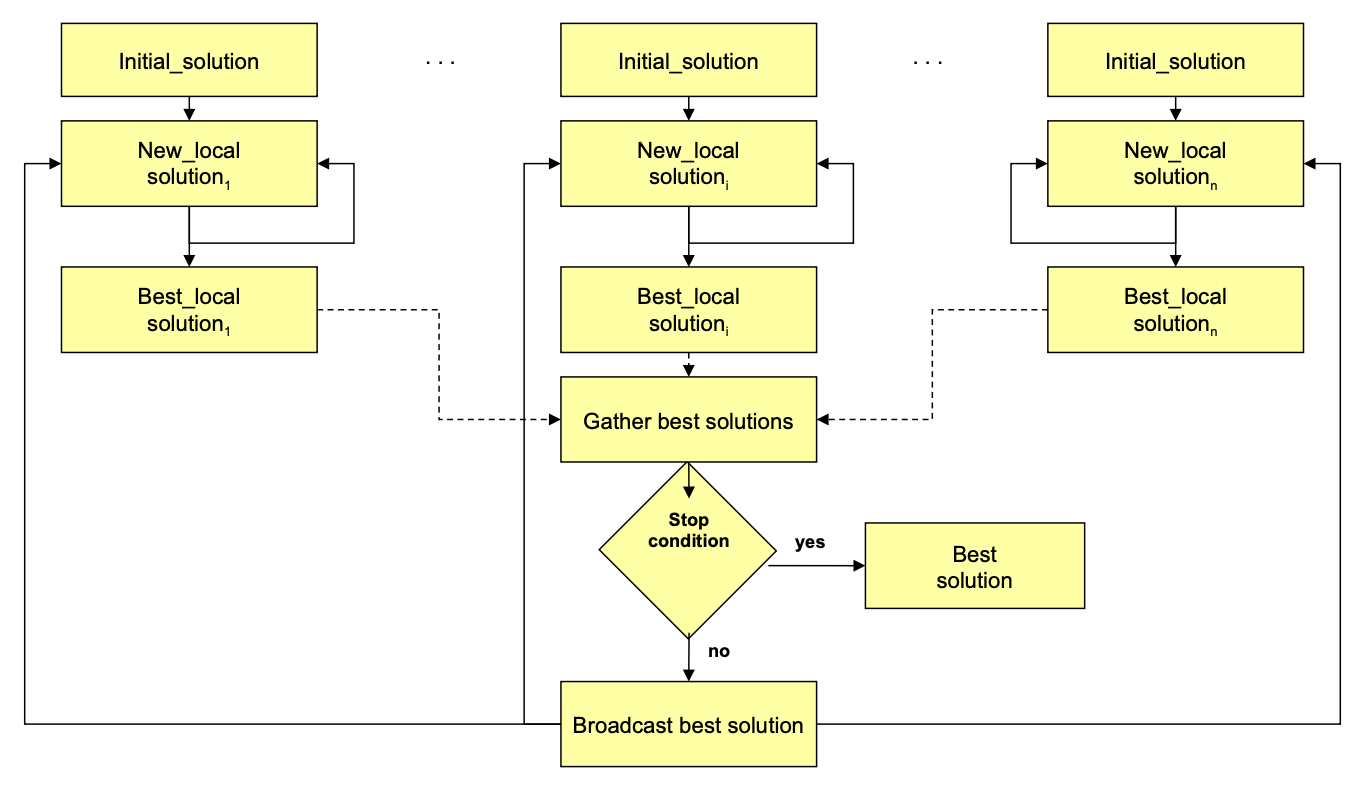
\includegraphics[width=0.8\textwidth]{pics/IOpar1.png}
        \caption{Схема асинхронного параллельного алгоритма имитации отжига}
        \label{fig:async}
    \end{figure}

    \item \textbf{Синхронная схема} (рис. \ref{fig:sync}):
    \begin{itemize}
        \item Процессоры синхронизируются на каждой итерации.
        \item Координатор собирает решения, выбирает глобально лучшее.
        \item Обеспечивает детерминированность, но увеличивает накладные расходы.
    \end{itemize}

    \begin{figure}[H]
        \centering
        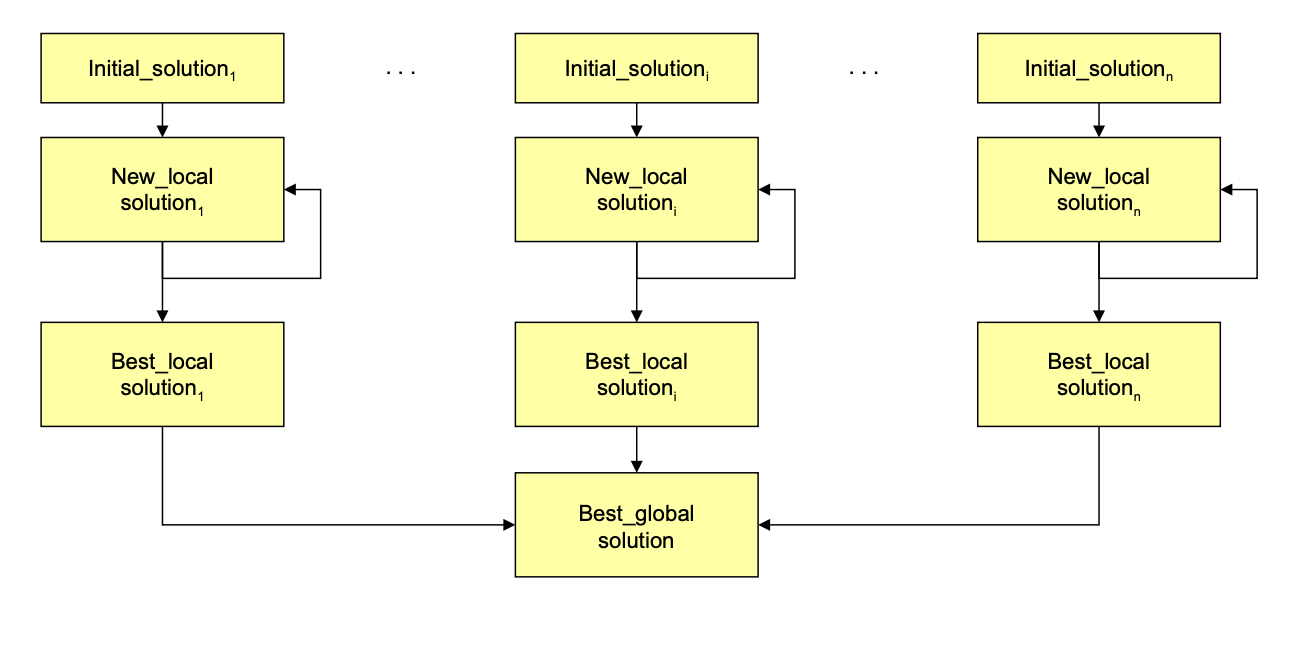
\includegraphics[width=0.8\textwidth]{pics/IOpar2.png}
        \caption{Схема синхронного параллельного алгоритма с координатором}
        \label{fig:sync}
    \end{figure}
\end{enumerate}

Дополнительные подходы:
\begin{itemize}
    \item \textbf{Декомпозиция целевой функции} — параллельное вычисление независимых компонент.
    \item \textbf{Разбиение пространства решений} — распределение областей поиска между узлами.
    \item \textbf{Гибридные стратегии} — комбинация распараллеливания с динамическим управлением $T$.
\end{itemize}


\bigbreak
[\cite{kostenko_lectures}]

\subsection{DOP 15 Основные  принципы  построения  и  архитектура  сети  Интернет.  Алгоритмы  и  протоколы  внешней  и внутренней маршрутизации. Явление перегрузки и методы борьбы с ней.}

\textbf{Основные принципы построения сети Интернет}

\begin{enumerate}
    \item \textit{Децентрализация управления} --- нет единого центра управления для сети Интернет.
    \item Выход из строя одного компьютера или участка сети не приводит к неработоспособности всей сети.
    \item \textit{Коммутация пакетов} --- способ динамического распределения ресурсов сети связи за счёт передачи и коммутации оцифрованной информации в виде частей небольшого размера, так называемых \textit{пакетов}, которые передаются по сети, в общем случае, независимо друг от друга (дейтаграммы) либо последовательно друг за другом по виртуальным соединениям. 
    Узел-приёмник из пакетов собирает сообщение. 
    В таких сетях по одной физической линии связи могут обмениваться данными много узлов.
    \item \textit{Инкапсуляция} --- последовательное вложение протокольной единицы (PDU) вышележащего уровня в протокольную единицу нижележащего уровня. 
    PDU вышележащего уровня не доступны на нижележащем уровне (нижележащий уровень не понимает структуры данных вышележащего уровня).
    \item Каждый уровень имеет строго определенный интерфейс с нижележащим и вышележащим уровнями и набор сервисов, которые может использовать вышележащий уровень.
\end{enumerate}

\bigbreak
\includegraphics[width=0.2\textwidth]{pics/protocols.png}

\textbf{ISO/OSI:}

\textbf{Физический} -- передача последовательности битов через физическую линию.

\textbf{Канальный} -- превращение несовершенной физической среды передачи данных в надежный канал, свободный от ошибок передачи.

\textbf{Сетевой} -- построение маршрута между отправителем и получателем.

\textbf{Транспортный} -- получение данных с вышерасположенного уровня, разделение на более мелкие единицы (если требуется), передача на сетевой уровень, обеспечение целостности данных при доставке до адресата.

\textbf{Сессии} -- установка сессий между пользователями. Сессия позволяет передавать данные, как это может делать транспортный уровень, и имеет более сложный сервис, полезный в некоторых приложениях. Например, можно осуществить вход в удаленную систему.

\textbf{Представления} -- обеспечение решений проблем, связанных с представлением данных, в основном — проблемы синтаксиса и семантики передаваемой информации.

\textbf{Приложений} -- обеспечение работы часто используемых приложений, например — передача файлов.


%\includegraphics[width=0.24\textwidth]{pics/iso_osi.jpg}
%(PDU -- Protocol Data Unit)

\bigbreak
\textbf{TCP/IP:}

\textbf{Прикладной уровень}.
На прикладном уровне (Application layer) работает большинство сетевых приложений.
Эти программы имеют свои собственные протоколы обмена информацией, например, интернет браузер для протокола HTTP, ftp-клиент для протокола FTP (передача файлов).

\textbf{Транспортный уровень} (как упаковывать?).
Протоколы транспортного уровня (Transport layer) могут решать проблему негарантированной доставки сообщений («дошло ли сообщение до адресата?»), а также гарантировать правильную последовательность прихода данных.

\textbf{Сетевой (межсетевой) уровень} (кому отправлять?).
Межсетевой уровень (Network layer) изначально разработан для передачи данных из одной сети в другую. На этом уровне работают маршрутизаторы, которые перенаправляют пакеты в нужную сеть путём расчёта адреса сети по маске сети.

\textbf{Канальный уровень} (как кодировать в среде?).
Канальный уровень (англ. Link layer) описывает способ кодирования данных для передачи пакета данных на физическом уровне (то есть специальные последовательности бит, определяющих начало и конец пакета данных, а также обеспечивающие помехоустойчивость).

% Снизу вверх: машина СПД (сети передачи данных), межсетевой уровень, транспортный уровень, уровень приложений.

% Модель никак не регламентирует организацию и функционирование сети передачи данных, ровно как и связь с ней, поэтому про уровень машины СПД сказать нечего.

% В модели нет уровня сессий и уровня представлений, поскольку необходимость в них была неочевидна для ее создателей. 

% Остальные уровни соответствуют одноименным уровням модели ISO/OSI.

\bigbreak
\textbf{Алгоритмы и протоколы внешней и внутренней маршрутизации}

Алгоритмы маршрутизации применяются для определения наилучшего пути пакетов от источника к приёмнику и являются основой протокола маршрутизации. 
Для формулирования алгоритмов маршрутизации сеть рассматривается как граф. 
При этом маршрутизаторы являются узлами, а физические линии между маршрутизаторами --- рёбрами соответствующего графа.
Каждой грани графа присваивается определённое число --- стоимость, зависящая от физической длины линии, скорости передачи данных по линии или стоимости линии.
Основными алгоритмами являются алгоритмы Беллмана-Форда и Дейкстры.

\textbf{Алгоритм Беллмана-Форда} (пример алгоритма по вектору расстояний):

\begin{itemize}
    \item Пусть каждый маршрутизатор знает стоимость линии к каждому своему непосредственному соседу
    \item Маршрутизатор $R_8$ рассчитывает стоимость $C_i$ для достижения каждого известного ему $R_i$
    \item Вектор $C_8 = (C_1,C_2,...,C_7)$ - вектор расстояния до $R_8$
    \item Изначально $C = (\infty,\infty,...,\infty)$
    \begin{enumerate}
        \item Каждые $T$ секунд $R_i$ шлёт $C_i$ всем свои соседям
        \item Если $R_i$ нашёл более дешёвый путь, то он обновляет $C_i$ у всех своих соседей
        \item Вернуться к 1
    \end{enumerate}
    \item Длину вектора $C$ устанавливает администратор
\end{itemize}

\textbf{Алгоритм Дейкстры} (пример алгоритма по состоянию канала):

\begin{enumerate}
    \item Определение топологии сети: каждый маршрутизатор передаёт лавиной всем своим соседям состояния своих линий и строит топлогию сети (1. Периодически, 2 Когда изменяется состояние линии)
    \item Вычисление по алгоритму Дейкстры: каждый маршрутизатор независимо запускает алгоритм Дейкстры наикратчайшего пути.
    Каждый маршрутизатор находит соединяющее дерево с минимальной стоимостью до каждого другого маршрутизатора.
\end{enumerate}

\textit{Протоколы внутренней маршрутизации}: RIP (на основе алгоритма Б-Ф, редко используется), OSPF (на основе алгоритма Д, широко используется).

\textit{Протоколы внешней маршрутизации}: BGP-4 --- алгоритм разработан для того, чтобы решить проблему того, что Интернет представляет из себя смесь разнообразных автономных сетей. Необходимо учитывать ряд условий, связанных с политикой автономной сети, например, пакеты из Министерства обороны не должны проходить через недружественные страны.


\textbf{Перегрузка} --- падение производительности в транспортной среде из-за слишком большого числа пакетов. (Если на маршрутизаторе в очереди скапливается много пакетов, то они просто сбрасываются -- это неэффективно)

\textbf{Управление перегрузками} --- организация потоков в транспортной среде, при которой потоки соответствуют пропускной способности подсети и не превышают ее.
% \begin{itemize}
%     \item \textit{Перегрузка} --- падение производительности в транспортной среде из-за слишком большого числа пакетов. (Если на маршрутизаторе в очереди скапливается много пакетов, то они просто сбрасываются -- это неэффективно)
%     \item \textit{Управление перегрузками} --- организация потоков в транспортной среде, при которой потоки соответствуют пропускной способности подсети и не превышают ее.
%     \item \textit{Методы, предотвращающие перегрузки:}
%     \begin{enumerate}
%         \item Схема управления потоком (небольшое окно) сдерживает нарастание трафика и предотвращает появление перегрузок.
%         \item Методы управления очередями, организация очередей: одна общая на входе или одна общая на выходе; по одной на каждую входную линию или на каждую выходную; по одной очереди на каждую входную и выходную --- все это влияет на появление перегрузок.
%         \item Выбор метода сброса пакетов также влияет на перегрузки. 
%         Правильная маршрутизация, равномерно использующая каналы в транспортной среде, позволяет избежать перегрузки.
%         \item Методы, регулирующие время жизни пакета в сети, также влияют на образование перегрузок.
%     \end{enumerate}
% \end{itemize}


\includegraphics[width=0.75\columnwidth]{pics/dop16_add.jpg}

\includegraphics[width=0.75\columnwidth]{pics/dop16_mul.jpg}

% -------- source --------
\bigbreak
[\cite{smelbook1}]
[\cite{smelbook2}]
\subsection*{DOP 17 Основные  принципы  построения  и  архитектура  сети  Интернет.  Алгоритмы  и  протоколы  внешней  и внутренней маршрутизации. Явление перегрузки и методы борьбы с ней.}

\textbf{Основные принципы построения сети Интернет}

\begin{enumerate}
    \item \textit{Децентрализация управления} --- нет единого центра управления для сети Интернет.
    \item Выход из строя одного компьютера или участка сети не приводит к неработоспособности всей сети.
    \item \textit{Коммутация пакетов} --- способ динамического распределения ресурсов сети связи за счёт передачи и коммутации оцифрованной информации в виде частей небольшого размера, так называемых \textit{пакетов}, которые передаются по сети, в общем случае, независимо друг от друга (дейтаграммы) либо последовательно друг за другом по виртуальным соединениям.
    Узел-приёмник из пакетов собирает сообщение.
    В таких сетях по одной физической линии связи могут обмениваться данными много узлов.
    \item \textit{Инкапсуляция} --- последовательное вложение протокольной единицы (PDU) вышележащего уровня в протокольную единицу нижележащего уровня.
    PDU вышележащего уровня не доступны на нижележащем уровне (нижележащий уровень не понимает структуры данных вышележащего уровня).
    \item Каждый уровень имеет строго определенный интерфейс с нижележащим и вышележащим уровнями и набор сервисов, которые может использовать вышележащий уровень.
\end{enumerate}

\bigbreak
\includegraphics[width=0.2\textwidth]{pics/protocols.png}

\textbf{ISO/OSI:}

\textbf{Физический} -- передача последовательности битов через физическую линию.

\textbf{Канальный} -- превращение несовершенной физической среды передачи данных в надежный канал, свободный от ошибок передачи.

\textbf{Сетевой} -- построение маршрута между отправителем и получателем.

\textbf{Транспортный} -- получение данных с вышерасположенного уровня, разделение на более мелкие единицы (если требуется), передача на сетевой уровень, обеспечение целостности данных при доставке до адресата.

\textbf{Сессии} -- установка сессий между пользователями. Сессия позволяет передавать данные, как это может делать транспортный уровень, и имеет более сложный сервис, полезный в некоторых приложениях. Например, можно осуществить вход в удаленную систему.

\textbf{Представления} -- обеспечение решений проблем, связанных с представлением данных, в основном — проблемы синтаксиса и семантики передаваемой информации.

\textbf{Приложений} -- обеспечение работы часто используемых приложений, например — передача файлов.


%\includegraphics[width=0.24\textwidth]{pics/iso_osi.jpg}
%(PDU -- Protocol Data Unit)

\bigbreak
\textbf{TCP/IP:}

\textbf{Прикладной уровень}.
На прикладном уровне (Application layer) работает большинство сетевых приложений.
Эти программы имеют свои собственные протоколы обмена информацией, например, интернет браузер для протокола HTTP, ftp-клиент для протокола FTP (передача файлов).

\textbf{Транспортный уровень} (как упаковывать?).
Протоколы транспортного уровня (Transport layer) могут решать проблему негарантированной доставки сообщений («дошло ли сообщение до адресата?»), а также гарантировать правильную последовательность прихода данных.

\textbf{Сетевой (межсетевой) уровень} (кому отправлять?).
Межсетевой уровень (Network layer) изначально разработан для передачи данных из одной сети в другую. На этом уровне работают маршрутизаторы, которые перенаправляют пакеты в нужную сеть путём расчёта адреса сети по маске сети.

\textbf{Канальный уровень} (как кодировать в среде?).
Канальный уровень (англ. Link layer) описывает способ кодирования данных для передачи пакета данных на физическом уровне (то есть специальные последовательности бит, определяющих начало и конец пакета данных, а также обеспечивающие помехоустойчивость).

% Снизу вверх: машина СПД (сети передачи данных), межсетевой уровень, транспортный уровень, уровень приложений.

% Модель никак не регламентирует организацию и функционирование сети передачи данных, ровно как и связь с ней, поэтому про уровень машины СПД сказать нечего.

% В модели нет уровня сессий и уровня представлений, поскольку необходимость в них была неочевидна для ее создателей.

% Остальные уровни соответствуют одноименным уровням модели ISO/OSI.

\bigbreak
\textbf{Алгоритмы и протоколы внешней и внутренней маршрутизации}

Алгоритмы маршрутизации применяются для определения наилучшего пути пакетов от источника к приёмнику и являются основой протокола маршрутизации.
Для формулирования алгоритмов маршрутизации сеть рассматривается как граф.
При этом маршрутизаторы являются узлами, а физические линии между маршрутизаторами --- рёбрами соответствующего графа.
Каждой грани графа присваивается определённое число --- стоимость, зависящая от физической длины линии, скорости передачи данных по линии или стоимости линии.
Основными алгоритмами являются алгоритмы Беллмана-Форда и Дейкстры.

\textbf{Алгоритм Беллмана-Форда} (пример алгоритма по вектору расстояний):

\begin{itemize}
    \item Пусть каждый маршрутизатор знает стоимость линии к каждому своему непосредственному соседу
    \item Маршрутизатор $R_8$ рассчитывает стоимость $C_i$ для достижения каждого известного ему $R_i$
    \item Вектор $C_8 = (C_1,C_2,...,C_7)$ - вектор расстояния до $R_8$
    \item Изначально $C = (\infty,\infty,...,\infty)$
    \begin{enumerate}
        \item Каждые $T$ секунд $R_i$ шлёт $C_i$ всем свои соседям
        \item Если $R_i$ нашёл более дешёвый путь, то он обновляет $C_i$ у всех своих соседей
        \item Вернуться к 1
    \end{enumerate}
    \item Длину вектора $C$ устанавливает администратор
\end{itemize}

\textbf{Алгоритм Дейкстры} (пример алгоритма по состоянию канала):

\begin{enumerate}
    \item Определение топологии сети: каждый маршрутизатор передаёт лавиной всем своим соседям состояния своих линий и строит топлогию сети (1. Периодически, 2 Когда изменяется состояние линии)
    \item Вычисление по алгоритму Дейкстры: каждый маршрутизатор независимо запускает алгоритм Дейкстры наикратчайшего пути.
    Каждый маршрутизатор находит соединяющее дерево с минимальной стоимостью до каждого другого маршрутизатора.
\end{enumerate}

\textit{Протоколы внутренней маршрутизации}: RIP (на основе алгоритма Б-Ф, редко используется), OSPF (на основе алгоритма Д, широко используется).

\textit{Протоколы внешней маршрутизации}: BGP-4 --- алгоритм разработан для того, чтобы решить проблему того, что Интернет представляет из себя смесь разнообразных автономных сетей. Необходимо учитывать ряд условий, связанных с политикой автономной сети, например, пакеты из Министерства обороны не должны проходить через недружественные страны.


\textbf{Перегрузка} --- падение производительности в транспортной среде из-за слишком большого числа пакетов. (Если на маршрутизаторе в очереди скапливается много пакетов, то они просто сбрасываются -- это неэффективно)

\textbf{Управление перегрузками} --- организация потоков в транспортной среде, при которой потоки соответствуют пропускной способности подсети и не превышают ее.
% \begin{itemize}
%     \item \textit{Перегрузка} --- падение производительности в транспортной среде из-за слишком большого числа пакетов. (Если на маршрутизаторе в очереди скапливается много пакетов, то они просто сбрасываются -- это неэффективно)
%     \item \textit{Управление перегрузками} --- организация потоков в транспортной среде, при которой потоки соответствуют пропускной способности подсети и не превышают ее.
%     \item \textit{Методы, предотвращающие перегрузки:}
%     \begin{enumerate}
%         \item Схема управления потоком (небольшое окно) сдерживает нарастание трафика и предотвращает появление перегрузок.
%         \item Методы управления очередями, организация очередей: одна общая на входе или одна общая на выходе; по одной на каждую входную линию или на каждую выходную; по одной очереди на каждую входную и выходную --- все это влияет на появление перегрузок.
%         \item Выбор метода сброса пакетов также влияет на перегрузки.
%         Правильная маршрутизация, равномерно использующая каналы в транспортной среде, позволяет избежать перегрузки.
%         \item Методы, регулирующие время жизни пакета в сети, также влияют на образование перегрузок.
%     \end{enumerate}
% \end{itemize}


\includegraphics[width=0.75\columnwidth]{pics/dop16_add.jpg}

\includegraphics[width=0.75\columnwidth]{pics/dop16_mul.jpg}

% -------- source --------
\bigbreak
[\cite{smelbook1}]
[\cite{smelbook2}]

\subsection*{DOP 18 Теоретические основы передачи данных, физический уровень стека протоколов. Системы передачи данных Ethernet и Wi-Fi: алгоритмы работы, управление множественным доступом к каналу}

\textbf{Теоретические основы}


\textbf{Данные} --- описание фактов, явлений.

\textbf{Сигнал} --- представление данных при передаче.

\textbf{Передача} --- процесс взаимодействия передатчика и приёмника, с целью передачи сигнала.
Данные и сигналы могут быть аналоговым (непрерывными) и цифровыми.
Для цифровой передачи данных сигнал нужно разбивать на уровни (для кодирования).

\textbf{Полоса пропускания канала} --- спектр частот, которые канал пропускает без существенного понижения мощности сигнала.

Скорость передачи зависит от способа кодирования данных на физическом уровне и \textbf{сигнальной скорости} -- скорости изменения значения сигнала.

\textbf{Пропускная способность канала} --- максимальная скорость, с которой канал способен передавать данные.

\bigbreak
\textbf{Теорема Найквиста-Котельникова}: $R_{max\_data\_rate} = 2*D*log_2{L}$ bps (bits per second)

- $R_{max\_data\_rate}$ - максимальная пропускная спсобность канала

- $D$ - ширина полосы пропускания канала (максимальная частота сигнала в спектре).

- $L$ - количество уровней (значений) сигнала.

\bigbreak
\textbf{Теорема Котельникова} --- Аналоговый сигнал $u(t)$, не содержащий частот выше $F_{max}$(Гц), полностью определяется последовательностью своих значений в моменты времени, отстоящие друг от друга на $\frac{1}{2F_{max}}$

\bigbreak
\textbf{Шум в канале} измеряется, как соотношение мощности полезного сигнала к мощности шума: $\frac{S}{N}$ (измеряется в децибелах $1dB = 10*\log_{10}{\frac{S}{N}}$)

\bigbreak
\textbf{Теорема Шеннона}: $R_{max} = D*log_2{(1+\frac{S}{N})}$ bps (bits per second)

- $R_{max}$ - максимальная скорость передачи данных по каналу с шумом

- $D$ - ширина полосы пропускания канала (максимальная частота сигнала в спектре).

- $\frac{S}{N}$ - соотношение сигнал-шум в канале,  $S$ - мощность сигнала, $N$ - мощность шума

\textbf{Характеристики физической среды}:
\begin{itemize}
    \item Полоса пропускания
    \item Пропускная способность
    \item Задержка
    \item Затухание
    \item Помехоустойчивость
    \item Достоверность передачи
    \item Стоимость
    \item Простота прокладки
    \item Сложность обслуживания
\end{itemize}


\textbf{\textbf{Ethernet}}

\begin{itemize}
    \item Узлы в сети Ethernet адресуются при помощи 6-байтового двоичного числа, называемого МАС-адресом (Media Access Control — управление доступом к носителю).
    \item Распределением МАС-адресов между производителями оборудования занимается международная некоммерческая организация IEEE (Institute of Elecrical and Electronics Engineers — Институт инженеров электротехники и электроники).
    \item Любой участник может послать в сеть сообщение, но только тогда, когда в ней <тихо> --- нет другой передачи.
    \item Ethernet использует протокол разрешения адресов (ARP) для определения MAC-адресов и их сопоставления с известными адресами сетевого уровня.
    \item У каждого узла в IP-сети есть МАС и IP-адреса.
    \item Узел должен использовать собственные МАС- и IP-адреса в полях источника, а также предоставить МАС и IP-адреса для назначения.
   \item  Несмотря на то, что IP-адрес назначения будет предоставлен более высоким уровнем OSI, отправляющему узлу необходимо найти MAC-адрес назначения для данного канала Ethernet.
    В этом заключается назначение протокола ARP.
\end{itemize}

\textbf{\textbf{Wi-Fi}}

\begin{itemize}
    \item Обычно схема сети Wi-Fi содержит не менее одной точки доступа и не менее одного клиента.
    \item Также возможно подключение двух клиентов в режиме точка-точка (Ad-hoc), когда точка доступа не используется, а клиенты соединяются посредством сетевых адаптеров <напрямую>.
    \item Точка доступа передаёт свой идентификатор сети (SSID -- Service Set Identifier) с помощью специальных сигнальных пакетов
    \item Зная SSID сети, клиент может выяснить, возможно ли подключение к данной точке доступа.
    \item При попадании в зону действия двух точек доступа с идентичными SSID приёмник может выбирать между ними на основании данных об уровне сигнала.
    \item Стандарт Wi-Fi даёт клиенту полную свободу при выборе критериев для соединения.
\end{itemize}

\textbf{\textbf{Управление множественным доступом}}

\begin{itemize}
    \item Проблема управления множественным доступом встаёт в тот момент, когда несколько отправителей хотят отправить свои данные через сеть.
    \item Протокол множественного доступа может определять и предотвращать коллизии пакетов (кадров) данных при условии, что в качестве режима конкурирующего доступа используется метод доступа к каналу, или зарезервированы ресурсы для установления логического канала.
    \item Механизм множественного доступа основан на схеме мультиплексирования (передача нескольких потоков данных с меньшей скоростью по одному каналу связи) физического уровня.
\end{itemize}
\textbf{Протоколы}:
\begin{itemize}
    \item \textbf{CSMA/CD (Carrier Sense Multiple Access with Collision Detection)}
    Если во время передачи кадра рабочая станция обнаруживает другой сигнал, занимающий передающую среду, она останавливает передачу, посылает сигнал преднамеренной помехи и ждёт в течение случайного промежутка времени (backoff delay), перед тем как снова отправить кадр.
    В Ethernet коллизии могут быть обнаружены сравнением передаваемой и получаемой информации. Если она различается, то другая передача накладывается на текущую (возникла коллизия) и передача прерывается немедленно. Посылается сигнал преднамеренной помехи, что вызывает задержку передачи всех передатчиков на произвольный интервал времени, снижая вероятность коллизии во время повторной попытки.
    Ethernet является классическим примером протокола CSMA/CD.
    \item \textbf{Aloha (чистая)}
    Отправитель начинает передавать, если в этот момент он слышит чужой сигнал, то он понимает, что произошло наложение и перестает передавать, ждет случайное время и начинает передавать сначала.
    В Wi-Fi суть та же.
    \item \textbf{Aloha (слотированная)}
    Модификация алохи. Все время работы канала разделяется на слоты. Размер слота при этом должен быть равен максимальному времени кадра. Такая организация работы канала требует синхронизации: одна из станций испускает сигнал начала очередного слота, поскольку передачу теперь можно начинать не в любой момент, а только по специальному сигналу, то время на обнаружение коллизии сокращается вдвое. Размер слота при этом должен быть равен максимальному времени кадра.
\end{itemize}

% -------- source --------
\bigbreak
[\cite[page 69-96]{smelbook2}]

\subsection{DOP 19 Базисные типы данных в языках программирования. Основные проблемы, связанные с базисными типами и способы их решения в различных языках. Понятие абстрактного типа данных и способы его реализации в современных языках программирования.}

\textbf{Простые типы данных и их свойства}

\textbf{Целые типы:}
\begin{itemize}
    \item Универсальность (насколько полно учтены машинные типы).
    \item Наличие (или отсутствие) беззнаковых типов (в Java их нет, в С++, С\# есть).
    \item Представление (размер значения, диапазоны значений).
    \item Надежность (какие ошибки могут возникать при выполнении операций с целыми значениями --- переполнение типа)
    \item Набор операций (почти во всех языках одинаково, в Java нет беззнакового типа, поэтому есть логический сдвиг).
\end{itemize}

\textbf{Вещественные типы:}
\begin{itemize}
    \item $(-1)^S \ast M \ast 2^p$, где $S$ --- бит знака, $M$ --- нормализованная мантисса ($0.5 \leq M < 1$), $p$ --- порядок.
    \item Неточные (например, \texttt{float} --- точность сложения $2^{-23}$ , если операнды между 0.5 и 1.
\end{itemize}

\textbf{Символьные типы:}
\begin{itemize}
    \item Включают в себя как символы алфавитов естественных языков, так и символы, управляющие работой устройств ввода/вывода, и специальные символы.
    \item Главной проблемой символьного типа является выбор кодировки.
    Современное решение --- Unicode.
\end{itemize}

\textbf{Логические типы:} в С отсутствует, в С++ можно преобразовывать к целому, в C\#, Java --- нет.

\textbf{Порядковые типы:}
\begin{itemize}
    \item \textit{Перечислимые типы} --- перечень именованных значений констант, \textit{типы диапазона}.
    \item \textit{Перечислимый тип С++}: числовые значения констант - всегда \texttt{int}, преобразования \texttt{enum} в \texttt{int} --- неявно, \texttt{int} в \texttt{enum} --- только явно, константы перечислимого типа имеют ту же область действия, что и имя перечислимого типа.
    \item \textit{Перечислимый тип C\#}: константы типа доступны через <имя типа>.<имя константы>, только явные преобразования между \texttt{enum} и \texttt{int}.
    \item \textit{Java}: аналогично C\# и являются классами.
    \item \textit{Тип диапазона} позволяет ограничить значения целого типа.
    Есть в Паскале, в С++, C\#, Java --- нет.
\end{itemize}

\textbf{Указательные и ссылочные типы данных:}
\begin{itemize}
    \item \textit{Указатель} абстракция понятия машинного адреса, есть в C, C++ --- может привести к хитрым ошибкам.
    Основные причины использования указателей: передача адресов объектов данных в подпрограммы, работа с объектами из динамической памяти.
    \item \textit{Ссылка} - абстракция понятия машинного адреса, лишенная недостатков указателя.
    Ссылки C\# и Java отличаются от ссылок С++ тем, что ссылка С++ ``навсегда'', то есть в течение всего времени жизни ссылки, полностью ассоциированы с объектом.
    Однако, и ссылки в С++, и ссылки в C\# и Java похожи в том смысле, что после установления ассоциации с объектом ссылка идентична самому объекту, поэтому не требуется никакая операция разыменования.
\end{itemize}

\textbf{Составные типы и их свойства}

\begin{enumerate}
    \item \textit{Одномерные массивы.}

    Массив — это непрерывная последовательность элементов одного типа.
    Атрибуты массива: базовый тип (T), тип индекса (I), диапазон индекса (L и R — нижняя и верхняя граница) и связанная с ним характеристика: длина массива.
    В С\# и Java массивы - полноправные объекты.
    \item \textit{Многомерные массивы.}

    В большинстве языков рассматриваются как массивы массивов.
    В Java все многомерные массивы --- ступенчатые (то есть внутренние массивы не обязаны иметь одну длину), в C\# есть прямоугольный массив (для более эффективного доступа к элементам и возможности обрабатывать массивы, совместимые с моделью данных языков типа С).
    \item \textit{Динамические строки.}

    Последовательность символов произвольной длины.
    Необходимость введения специального типа вместо массива: строки реализуются как неизменяемый объект (главный аргумент), набор операций для строк существенно шире и специфичней набора операций для обычных массивов.
    \item \textit{Записи (структуры)} --- это совокупность объявлений переменных, которые объединены в отдельный объект.
\end{enumerate}

\textbf{Абстрактные типы данных}

\textit{Абстрактный тип данных (АТД)} --- тип, в котором внутренняя структура данных полностью инкапсулирована, то есть тип представлен только множеством операций.
Класс является абстрактным типом данных, если открытыми членами являются только методы.

Говорят, что совокупность открытых членов класса составляет \textit{интерфейс} класса.

\textit{Реализация:}
\begin{itemize}
    \item Сокрытие членов-данных, доступ через селекторы (геттеры-сеттеры) или их абстракцию --- свойство (в C\#).
    \item \textit{Абстрактный класс} --- класс, который предназначен исключительно для того, чтобы быть базовым классом.
    \item \textit{Интерфейс} --- класс, состоящий только из абстрактных методов.
\end{itemize}

% -------- source --------
\bigbreak
[\cite{golovin}]

\subsection{Основные  характеристики  функциональных  языков  программирования.  Использование  понятий функционального  программирования  (замыкания,  анонимные функции)  в  современных  объектно-ориентированных языках.}

\textbf{Свойства функциональных ЯП:}
\begin{enumerate}
    \item Язык динамический --- связывания происходят во время выполнения.
    \item Нет понятия состояния и присваивания.
    \item Главная операция --- вызов функции.
    \item Главная абстракция --- определение функции.
    \item Функции --- объекты 1 класса, то есть могут быть значениями, вычисляться, передаваться как параметры и возвращаемые значения и т.п.
    \item Структуры данных --- списки (последовательности).
    \item Простая типовая структура.
    \item Понятие переменной соответствует математическому смыслу --- переменная отождествляется со значением, а не хранит его.
\end{enumerate}

\textbf{Понятия функционального программирования}

\begin{itemize}
    \item Замыкание --- это конструкция, которая связывает функцию (функциональное значение) с переменными из объемлющей области видимости.
    Про такие переменные говорят, что они ``захвачены'', их область видимости (scope) не совпадает с областью действия (extent), последняя --- шире.
    Пример:
    \begin{lstlisting}
function initAdder(x) {
    function adder(y) {return x + y}
    return adder
}
    \end{lstlisting}
    \item Анонимная функция (лямбда-функция) --- это ``чистое'' функциональное значение без имени. 
    Его можно передавать как параметр другой функции, возвращать как результат другой функции, в языках с процедурными конструкциями --- присваивать.
\end{itemize}

\textbf{Использование понятий ФП в современных ОО языках}

\textit{C\#}

\begin{lstlisting}
delegate(int x, int y) {return x+y;}
(x,y)=> {return x+y;}
(x,y)=>x+y
\end{lstlisting}

Лямбда-выражения (3 строчка) --- более общая конструкция, чем лямбда-операторы, могут быть преобразованы в стандартный тип деревьев выражений. 
Параметры анонимных делегатов типизированы (тип возвращаемого значения выводится из типа выражения в return). 
А лямбда-конструкции --- нетипизированы.

\textit{Java}

\begin{lstlisting}[language=Java]
(Integer x, Integer y) -> x + y 
\end{lstlisting}
или
\begin{lstlisting}[language=Java]
(Integer x, Integer y) -> return x + y; 
\end{lstlisting}
--- лямбда-выражения. 
Типами параметров лямбда-выражений могут быть только объектные типы, тип возвращаемого значения выводится из возвращаемых выражений.

Пример замыкания:

\begin{lstlisting}[language=Java]
Function<Integer, Integer> initAdder(int x) {
    return (Integer y) -> x + y;
}
\end{lstlisting}

\textbf{Пример на Python}:

\begin{lstlisting}[language=Python]
square = lambda n: n * n   # lambda expression
print(square(4))  # 16
\end{lstlisting}

% -------- source --------
\bigbreak
[\cite{golovin}]
\subsection*{DOP 21 Основные  характеристики  функциональных  языков  программирования.  Использование  понятий функционального  программирования  (замыкания,  анонимные функции)  в  современных  объектно-ориентированных языках.}

\textbf{Свойства функциональных ЯП:}
\begin{enumerate}
    \item Язык динамический --- связывания происходят во время выполнения.
    \item Нет понятия состояния и присваивания.
    \item Главная операция --- вызов функции.
    \item Главная абстракция --- определение функции.
    \item Функции --- объекты 1 класса, то есть могут быть значениями, вычисляться, передаваться как параметры и возвращаемые значения и т.п.
    \item Структуры данных --- списки (последовательности).
    \item Простая типовая структура.
    \item Понятие переменной соответствует математическому смыслу --- переменная отождествляется со значением, а не хранит его.
\end{enumerate}

\textbf{Понятия функционального программирования}

\begin{itemize}
    \item Замыкание --- это конструкция, которая связывает функцию (функциональное значение) с переменными из объемлющей области видимости.
    Про такие переменные говорят, что они ``захвачены'', их область видимости (scope) не совпадает с областью действия (extent), последняя --- шире.
    Пример:
    \begin{lstlisting}
function initAdder(x) {
    function adder(y) {return x + y}
    return adder
}
    \end{lstlisting}
    \item Анонимная функция (лямбда-функция) --- это ``чистое'' функциональное значение без имени.
    Его можно передавать как параметр другой функции, возвращать как результат другой функции, в языках с процедурными конструкциями --- присваивать.
\end{itemize}

\textbf{Использование понятий ФП в современных ОО языках}

\textit{C\#}

\begin{lstlisting}
delegate(int x, int y) {return x+y;}
(x,y)=> {return x+y;}
(x,y)=>x+y
\end{lstlisting}

Лямбда-выражения (3 строчка) --- более общая конструкция, чем лямбда-операторы, могут быть преобразованы в стандартный тип деревьев выражений.
Параметры анонимных делегатов типизированы (тип возвращаемого значения выводится из типа выражения в return).
А лямбда-конструкции --- нетипизированы.

\textit{Java}

\begin{lstlisting}[language=Java]
(Integer x, Integer y) -> x + y
\end{lstlisting}
или
\begin{lstlisting}[language=Java]
(Integer x, Integer y) -> return x + y;
\end{lstlisting}
--- лямбда-выражения.
Типами параметров лямбда-выражений могут быть только объектные типы, тип возвращаемого значения выводится из возвращаемых выражений.

Пример замыкания:

\begin{lstlisting}[language=Java]
Function<Integer, Integer> initAdder(int x) {
    return (Integer y) -> x + y;
}
\end{lstlisting}

\textbf{Пример на Python}:

\begin{lstlisting}[language=Python]
square = lambda n: n * n   # lambda expression
print(square(4))  # 16
\end{lstlisting}

% -------- source --------
\bigbreak
[\cite{golovin}]

% -+- используется в dop 22
\newcommand{\notsure}[1]{(видимо: #1)}
\newcommand{\aboba}[2]{\textbf{\LARGE dop #1. #2}}
\newcommand{\multicom}[1]{}
\newcommand{\lulz}[1]{}
\newcommand{\wantsayInstead}[1]{}
% -+-

\subsection*{DOP 22 Синхронизация  в  распределенных  системах.  Синхронизация  времени.  Логические  часы.  Выборы координатора. Взаимное исключение. Координация процессов.}

\bigbreak

\centerline{\textbf{Основное}}

\textit{Распределенная (компьютерная) система} (РС) --– совокупность связанных
сетью независимых компьютеров, которая представляется
пользователю единым компьютером.

% Черты РС:
% \begin{itemize}
%     \item конкурентность \notsure{доступ к ресурсам};
%     \item отсутствие глобальных часов;
%     \item независимые отказы.
% \end{itemize}

Свойства децентрализованных алгоритмов:
\vspace{-0.7em}
\begin{enumerate}
\setlength\itemsep{-0.4em}
\item используемая информация распределена среди множества ЭВМ;
\item процессы действуют на основе только локальной информации;
\item отсутствие критического узла, выход из строя которого приводит к краху алгоритма;
% eq:up \item не должно быть единственной критической точки, выход из строя которой приводил бы к краху алгоритма;
\item отсутствие общего источника глобального времени.
\end{enumerate}
пункты 1--3 о недопустимости хранения всей информации необходимой для принятия решения в одном место.


\centerline{\textbf{Синхронизация времени}}
%\begin{itemize}

$\circ$
\textbf{Аппаратные часы} --- счетчик временных сигналов и регистр с начальным значением счетчика [из слайдов].
\\
(\textit{Аппаратные часы} --- счетчик времени, система содержащая автономный источник питания и регистр. [из вики]).
%\wantsayInstead{\textit{Аппаратные часы} --- счетчик времени, система из автономного источника питания и регистра.}

$\circ$
Отношение ``произошло до'' ($\rightarrow$): $a \rightarrow b$ означает, что все процессы согласны, что сначала произошло событие $a$, а затем $b$.
Оно очевидно в 2--х случаях:
\vspace{-0.7em}
\begin{itemize}
    \setlength\itemsep{-0.4em}
    \item \lulz{аб}оба события ($a$ и $b$) произошли в одном процессе;
    \item событие $a$ --- отправка сообщения $m$, событие $b$ - прием $m$.
\end{itemize}

Отношение $\rightarrow$ транзитивно ($a \rightarrow b$ и $b \rightarrow c$ тогда $a \rightarrow c$).

Если события $x$ и $y$ произошли в разных процессах, не обменивающихся сообщениями, то отношения $x \rightarrow y$ и $y \rightarrow x$ неверны.
Такие события $x$ и $y$ называются \textit{одновременными}.

$\circ$
\textbf{\textit{Логические часы}} --- согласованное (между ЭВМ РС) время (потенциально) не имеющее ничего общего с астрономическим временем.

Введем логическое время $C$ следующим образом: если $a \rightarrow b$, то $C(a) < C(b)$.
Логические часы используют следующий алгоритм:
\begin{enumerate}
\item
Часы $C_i$ увеличивают свое значение с каждым событием в процессе $P_i$:
$C_i = C_i + d$, где $d > 0$ (обычно $1$).

\item
Если событие $a$ --- отправка сообщения $m$ процессом $P_i$, то в него добавляется временная метка $t_m=C_i(a)$.
При получении сообщения $m$ процессом $P_j$ его время корректируется: \\ $C_j = max(C_j,t_m + d$).
\end{enumerate}
%\end{itemize}

\centerline{\textbf{Выбор координатора}}

Многие распределенные алгоритмы требуют, чтобы один из процессов выполнял функции координатора. Рассмотрим алгоритмы выбора координатора.
\begin{enumerate}
\item
Алгоритм ``Задира'':
\begin{itemize}
    \setlength\itemsep{-0.4em}
    \item Если процесс $P$ обнаружит, что координатор долго не отвечает, то он инициирует выборы.
    \item $P$ посылает сообщение ``ВЫБОРЫ'' всем процессам с большими чем у него номерами.
    \item Если нет ни одного ответа, то $P$ считается победителем и становится координатором.
    \item Если один из процессов с большим номером ответит, то он берет на себя проведение выборов. Участие процесса $P$ в выборах заканчивается.
    \item В любой момент процесс может получить сообщение ``ВЫБОРЫ'' (от процесса с меньшим номером). В этом случае он посылает ответ ``OK'', чтобы сообщить, что он жив и берет проведение выборов на себя.
    \item Победитель извещает всех о своей победе сообщением ``КООРДИНАТОР''.
    \item (Сомнительный пункт: типа зачем, если новый координатор умрет, то управление вернется) Если бывший координатор восстановился после сбоя, то он проводит выборы.
\end{itemize}

\item
Круговой алгоритм:
\begin{itemize}
\item
Каждый процесс знает следующего за ним в круговом списке.
\item
Когда процесс обнаруживает отсутствие координатора, он посылает следующему за ним процессу сообщение ``ВЫБОРЫ'' со своим номером.
\item
Если следующий процесс не отвечает, то сообщение посылается процессу, следующему за ним, и т.д., пока не найдется работающий процесс.
\item
Каждый работающий процесс добавляет в список работающих свой номер и переправляет сообщение дальше по кругу.
\item
Когда процесс обнаружит в списке свой собственный номер (круг пройден), он меняет тип сообщения на ``КООРДИНАТОР'' и оно проходит по кругу, извещая всех о списке работающих и координаторе.
\end{itemize}
\end{enumerate}


\centerline{\textbf{Взаимное исключение}}

Речь о доступе к ресурсам. Рассмотрим несколько алгоритмов:
\begin{enumerate}
\item
Централизованный алгоритм.
\begin{itemize}
\item
Все процессы запрашивают у координатора разрешение на вход в критическую секцию и ждут этого разрешения.
\item
Координатор обслуживает запросы в порядке поступления.
\item
Получив разрешение процесс входит в критическую секцию.
\item
При выходе из нее он сообщает об этом координатору.
\end{itemize}
Кол--во сообщ. на одно прохождение критической секции --- 3.
\\
Недостатки алгоритма --- крах координатора или его перегрузка сообщениями.

\item
Алгоритм с круговым маркером.
\begin{itemize}
\item Каждый процесс знает следующего за ним в круговом списке.
\item По кольцу циркулирует маркер, дающий право на вход в критическую секцию.
\item Получив маркер (специальное сообщение) процесс либо входит в критическую секцию, либо переправляет маркер дальше.
\item После выхода из критической секции маркер переправляется дальше.
\end{itemize}

\item
Децентрализованный алгоритм на основе временных меток.
\\
Необх. глобальное упорядочение всех событий в сист. по времени.

Вход в критическую секцию:
\begin{itemize}
\item
Когда процесс желает войти в критическую секцию, он посылает всем процессам сообщение-запрос, содержащее имя критической секции, номер процесса и текущее время.
\item После посылки запроса процесс ждет, пока все дадут ему разрешение.
\item После получения от всех разрешения, он входит в критическую секцию.
\end{itemize}

Поведение процесса при приеме запроса:
\begin{itemize}
\item
Если получатель не находится внутри критической секции и не запрашивал разрешение на вход в нее, то он посылает отправителю сообщение``OK''.
\item
Если получатель находится внутри критической секции, то он не отвечает, а запоминает запрос.
\item
Если получатель выдал запрос на вхождение в эту секцию, но еще не вошел в нее, то он сравнивает временные метки своего запроса и чужого.
Побеждает тот, чья метка меньше.
Если чужой запрос победил, то процесс посылает сообщение ``OK''.
Если у чужого запроса метка больше, то ответ не посылается, а чужой запрос запоминается.
\end{itemize}

Выход из критической секции:
\begin{itemize}
\item
После выхода из секции он посылает сообщение «OK» всем процессам, запросы от которых он запомнил, а затем стирает все запомненные запросы.
\end{itemize}

Количество сообщений на одно прохождение секции --- $2(n-1)$, где n --- число процессов.
%\\
Если какой-то процесс перестанет функционировать, то отсутствие разрешения от него всех остановит.
% \\
Если в централизованном алгоритме есть опасность перегрузки координатора, то в этом алгоритме перегрузка любого процесса приведет к тем же последствиям.


%not uncom
%\item И еще несколько алгоритмов смотри ниже (писать не предлагаю), под чертой, в секции Cringe пункты 1--3.

\end{enumerate}

\centerline{\textbf{Координация процессов}}
\begin{enumerate}
\item  Если известен и ``потребитель'' и ``производитель'':
\begin{itemize} \item cообщения точка--точка. \end{itemize}
\item Если \textbf{НЕ}известен ``потребитель'':
\begin{itemize}
    \item широковещательные сообщения;
    \item сообщения в ответ на запрос.
\end{itemize}
\item Если \textbf{НЕ}известен и ``потребитель'' и ``производитель'' :
\begin{itemize}
    \item сообщения и запросы через координатора:
    \item широковещательный запрос.
\end{itemize}
\end{enumerate}

%\hrulefill

%\textbf{Cringe}
% У вас не захотят это спрашивать, вы не захотите это рассказывать:
% %\begin{enumerate}
% \\$\circ$%\item
% Децентрализованный алгоритм на основе временных меток.
% \\
% Требуется глобальное упорядочение всех событий в системе по времени.
% \begin{enumerate}

% \item
% Вход в критическую секцию:
% \begin{itemize}
% \item
% Когда процесс желает войти в критическую секцию, он посылает всем процессам сообщение-запрос, содержащее имя критической секции, номер процесса и текущее время.
% \item После посылки запроса процесс ждет, пока все дадут ему разрешение.
% \item После получения от всех разрешения, он входит в критическую секцию.
% \end{itemize}

% \item
% Поведение процесса при приеме запроса:
% \begin{itemize}
% \item
% Если получатель не находится внутри критической секции и не запрашивал разрешение на вход в нее, то он посылает отправителю сообщение``OK''.
% \item
% Если получатель находится внутри критической секции, то он не отвечает, а запоминает запрос.
% \item
% Если получатель выдал запрос на вхождение в эту секцию, но еще не вошел в нее, то он сравнивает временные метки своего запроса и чужого.
% Побеждает тот, чья метка меньше.
% Если чужой запрос победил, то процесс посылает сообщение ``OK''.
% Если у чужого запроса метка больше, то ответ не посылается, а чужой запрос запоминается.
% \end{itemize}

% \item
% Выход из критической секции:
% \begin{itemize}
% \item
% После выхода из секции он посылает сообщение «OK» всем процессам, запросы от которых он запомнил, а затем стирает все запомненные запросы.
% \end{itemize}
% \end{enumerate}
% Количество сообщений на одно прохождение секции - 2(n-1), где n - число процессов.
% \\
% Если какой-то процесс перестанет функционировать, то отсутствие разрешения от него всех остановит.
% \\
% И, наконец, если в централизованном алгоритме есть опасность перегрузки координатора, то в этом алгоритме перегрузка любого процесса приведет к тем же последствиям.



% \item
% Алгоритм широковещательный маркерный (прям уверен что это писать не стоит):
% \\
% Маркер содержит:
% \begin{itemize}
% \item очередь запросов;
% \item массив $LN[1...N]$ с номерами последних удовлетворенных запросов.
% \end{itemize}
% Сам Алгоритм:
% \begin{itemize}
% \item
% Вход в критическую секцию
% \begin{itemize}
% \item
% Если процесс $P_k$, запрашивающий критическую секцию, не имеет маркера, то он увеличивает порядковый номер своих запросов $RN_k[k]$ (я не ебу кто такой $RN_k$) и посылает широковещательно сообщение ``ЗАПРОС'', содержащее номер процесса $k$ и номер запроса $S_n = RN_k[k]$.
% \item
% Процесс $P_k$ выполняет критическую секцию, если имеет (или когда получит) маркер.
% \end{itemize}
% \item
% Поведение процесса при приеме запроса
% \begin{itemize}
% \item
% Когда процесс $P_j$ получит сообщение-запрос от процесса $P_k$, он
% устанавливает $RN_j[k]=max(RN_j[k],S_n)$. Если Pj имеет свободный маркер,
% то он его посылает $P_k$ только в том случае, когда $RN_j[k]==LN[k]+1$
% (запрос не старый).
% \end{itemize}
% \item
% Выход из критической секции процесса $P_k$.
% \begin{itemize}
% \item Устанавливает $LN[k]$ в маркере равным $RN_k[k]$.
% \item Для каждого $P_j$, для которого $RN_k[j]=LN[j]+1$, он добавляет его идентификатор в маркерную очередь запросов (если там его еще нет).
% \item Если маркерная очередь запросов не пуста, то из нее удаляется первый элемент, а маркер посылается соответствующему процессу (запрос которого был первым в очереди).
% \end{itemize}
% \end{itemize}

% \item
% Алгоритм древовидный маркерный.
% \\
% Все процессы представлены в виде сбалансированного двоичного дерева.
% Каждый процесс имеет очередь запросов от себя и соседних процессов (1-ого,
% 2-х или 3-х) и указатель в направлении владельца маркера.
% \\
% Критическая секция --- КС.
% \\
% Сам алгоритм:
% \begin{itemize}
% \item Вход в критическую секцию
% \begin{itemize}
%     \item Если есть маркер, то процесс выполняет КС.
%     \item Если нет маркера, то процесс:
% \begin{itemize}
%     \item помещает свой запрос в очередь запросов.
%     \item посылает сообщение «ЗАПРОС» в направлении владельца маркера и ждет сообщений.
% \end{itemize}
% \end{itemize}
% \item
% Поведение процесса при приеме сообщений.
% \\
% Процесс, не находящийся внутри КС должен реагировать на сообщения двух
% видов ``МАРКЕР'' и ``ЗАПРОС''.
% \begin{itemize}
%     \item
% Пришло сообщение ``МАРКЕР'':
% \begin{itemize}
% \item пункт $M1$.
% Взять 1-ый запрос из очереди и послать маркер его автору (концептуально, возможно себе);
% \item  Поменять значение указателя в сторону маркера;
% \item  Исключить запрос из очереди;
% \item  Если в очереди остались запросы, то послать сообщение ``ЗАПРОС'' в сторону маркера.
% \end{itemize}
% \item
% Пришло сообщение ``ЗАПРОС''.
% \begin{itemize}
%     \item  Поместить запрос в очередь.
%     \item  Если нет маркера, то послать сообщение ``ЗАПРОС'' в сторону маркера,
% иначе (если есть маркер) - перейти на пункт М1.
% \end{itemize}
% \end{itemize}
% \end{itemize}

% \item
% Выход из критической секции:
% \\
% Если очередь запросов пуста, то при выходе ничего не делается, иначе - перейти к пункту М1.
% \end{enumerate}


% -------- source --------
\bigbreak
[\cite[КонспектЛекций.zip/3-4-MPI-Sync.doc: page 8--15]{keldysh_ros_2021}]

\subsection*{DOP 23 Отказоустойчивость  в  распределенных  системах.  Типы  отказов.  Фиксация  контрольных  точек  и восстановление после отказа. Репликация и протоколы голосования. Надежная групповая рассылка.}

\textbf{Основные определения}

\begin{itemize}
    \item \textbf{Отказом системы} называется поведение системы, не удовлетворяющее ее спецификациям.
    Отказы могут быть случайными, периодическими или постоянными.
    Случайные отказы (сбои) при повторении операции исчезают.
    Отказы по характеру своего проявления: <византийские> (система активна, но некорректно работает), 2) <пропажа признаков жизни> (частичная или полная).

    Два подхода - восстановление решения после отказа системы (или ее компонента) и предотвращение отказа системы (отказоустойчивость).

    \textit{Восстановление:}
    \begin{enumerate}
        \item Прямое --- основано на своевременном обнаружении сбоя и ликвидации его последствий путем приведения некорректного состояния системы в корректное.
        Такое восстановление возможно только для определенного набора заранее предусмотренных сбоев.
        \item Возвратное --- возврат процесса (или системы) из некорректного состояния в некоторое из предшествующих корректных состояний.
    \end{enumerate}

    \includegraphics[width=0.24\textwidth]{pics/effect_domino.png}

    На рисунке показаны три процесса (X,Y,Z), взаимодействующие через сообщения. Вертикальные черточки показывают на временной оси моменты запоминания состояния процесса для восстановления в случае отказа. Стрелочки соответствуют сообщениям и показывают моменты их отправления и получения. Предположим теперь, что процесс Z сломается и будет восстановлен в состояние z2. Это приведет к откату процесса Y в y1, а затем и процессов X и Z в начальные состояния x1 и y1. Этот эффект известен как эффект домино.

    \item Множество контрольных точек называется \textbf{строго консистентным}, если во время его фиксации никаких обменов между процессами не было.
    Оно соответствует понятию строго консистентного глобального состояния, когда все посланные сообщения получены и нет никаких сообщений в каналах связи.
    \item Множество контрольных точек называется \textbf{консистентным}, если для любой зафиксированной операции приема сообщения, соответствующая операция посылки также зафиксирована (нет сообщений-сирот).
\end{itemize}

\textbf{Методы фиксации контрольных точек}

\begin{enumerate}
    \item \textbf{Простой метод} --- фиксация локальной контрольной точки после каждой операции посылки сообщения.
    При этом посылка сообщения и фиксация должны быть единой неделимой операцией (транзакцией).
    Множество последних локальных контрольных точек является консистентным (но не строго консистентным).

    Чтобы избежать потерь сообщений при восстановлении с использованием консистентного множества контрольных точек необходимо повторить отправку тех сообщений, квитанции о получении которых стали недействительными в результате отката.
    Используя временные метки сообщений можно распознавать сообщения-призраки.
    \item \textbf{Синхронная фиксация.}
    Два вида контрольных точек - постоянные и пробные.

    \textbf{Постоянная контрольная точка} --- это локальная контрольная точка, являющаяся частью консистентной глобальной контрольной точки.
    \textit{Пробная контрольная точка} --- это временная контрольная точка, которая становится постоянной только в случае успешного завершения алгоритма.

    \textbf{Фиксация}: \textit{1 фаза}.
    Инициатор фиксации (процесс $P_i$) создает пробную КТ и просит все остальные процессы сделать то же самое.
    При этом процессу запрещается посылать неслужебные сообщения после того, как он сделает пробную контрольную точку.
    Каждый процесс извещает $P_i$ о том, сделал ли он пробную КТ.
    Если все процессы сделали пробные контрольные точки, то $P_i$ превращает пробные точки в постоянные.
    Если какой-либо процесс не смог сделать пробную точку, все точки отменяются.

    \textit{2 фаза}. $P_i$ информирует все процессы о своем решении.

    \textbf{Восстановление}: \textit{1 фаза}.
    Инициатор отката спрашивает остальных, готовы ли они откатываться.
    Когда все будут готовы к откату, откат.

    \textit{2 фаза}.
    $P_i$ сообщает всем о принятом решении.
    Получив это сообщение, каждый процесс поступает указанным образом.
    С момента ответа на опрос готовности и до получения принятого решения процессы не должны посылать сообщения.
    \item \textbf{Асинхронная фиксация.}
    Множество контрольных точек может быть неконсистентным.
    При откате происходит поиск подходящего консистентного множества путем поочередного отката каждого процесса в ту точку, в которой зафиксированы все посланные им и полученные другими сообщения.
\end{enumerate}

\textbf{Репликация} - механизм синхронизации содержимого нескольких копий объекта

Рассмотрим возможные протоколы работоспособности коммуникаций и процессоров:

\begin{itemize}
    \item \textit{Протокол принятия единых решений}.

    Все исполнители являются исправными и должны либо все принять, либо все не принять заранее предусмотренное решение.

    \item \textit{Протокол принятия согласованных решений}.

    Наоборот, принятие решения при надежных коммуникациях, но ненадежной работы процессоров.
    В системе с $m$ неверно работающими процессорами можно достичь согласия только при наличии $2m+1$ верно работающих процессоров (более $2/3$) (задача Византийских генералов).
\end{itemize}

Предположим, что коммуникации надежны, а процессоры нет.

\textit{Алгоритм надежных неделимых широковещательных рассылок сообщений:}
\begin{description}
    \item[\textit{Фаза 1}] Процесс-отправитель посылает сообщение группе процессов (список их идентификаторов содержится в сообщении).
    Процессы приписывают сообщению приоритет и помещают в очередь (как недоставленное), информируют отправителя.
    \item[\textit{Фаза 2}] Отправитель получил все ответы => выбирает максимальный полученный приоритет и присваивает его сообщению, рассылает всем процессам.
    Получатели принимают, помечают сообщение как доставленное, упорядочивают сообщения в своих очередях.
    \item[] Если получатель обнаружит, что он имеет сообщение с пометкой <недоставленное>, отправитель которого сломался, то он для завершения выполнения протокола осуществляет следующие два шага в качестве координатора: опрашивает всех о статусе сообщения; получив все ответы, реагирует на них.
    Если сообщение у какого-то получателя помечено как <доставленное>, то его окончательный приоритет рассылается всем.
    Получив это сообщение каждый процесс выполняет шаги фазы 2.
    Иначе координатор заново начинает весь протокол с фазы 1.
\end{description}


% -------- source --------
\bigbreak
[\cite{parallel_lec7}]

\subsection{Промежуточные  представления  программы:  абстрактное  синтаксическое  дерево;  последовательность трехадресных инструкций. Базовые блоки и граф потока управления.}

\textbf{Промежуточное представление программы} (Intermediate Representation, IR) --- форма представления программы, ориентированная на удобство дальнейшей обработки компилятором.

Различают следующие IR:
\begin{itemize}
    \item HIR (высокий уровень) --- абстрактное синтаксическое дерево(АСД) --- конечное помеченное ориентированное дерево, в котором внутренние вершины сопоставлены (помечены) с операторами языка программирования, а листья --- с соответствующими операндами. По сути результат парсинга программы на языке программирования, по АСД можно однозначно восстановить программу, по остальным уже нельзя.
    \item MIR (средний уровень) --- включает в себя:
    \begin{enumerate}
        \item Инструкции
        \item[--] присваивание: \texttt{x <- op y z; x <- op y; x <- y;}
        \texttt{x[i] <- y; x <- y[i];},
        \item[--] переходы: \texttt{goto L; ifTrue x goto L; ifFalse x goto L;}
        \item[--] дополнительное: \texttt{param x; call x n; return y;}
        \item таблицу символов,
        \item[--] переменные, их имена в программе и атрибуты, такие как область видимости, тип, для имен функций - число параметров, и т. п.
    \end{enumerate}
    \item LIR (низкий уровень) --- фактически машинные инструкции --- используется для машинно-зависимых задач, например, распределение регистров и выбор подходящих команд.
\end{itemize}

\textbf{Базовые блоки и граф потока управления}

\textbf{Базовым блоком} (ББ или линейным участком) называется последовательность следующих одна за другой инструкций MIR, обладающая следующими свойствами:
\begin{itemize}
    \item Поток управления может входить в базовый блок только через его первую инструкцию (т.е. в программе нет переходов в середину базового блока),
    \item Поток управления покидает базовый блок без останова или ветвления, кроме, возможно, последней инструкции базового блока.
\end{itemize}

Грубо говоря, \textit{базовый блок} содержит инструкции, которые будут выполнены (или не выполнены) обязательно все вместе, независимо ни от чего. Поэтому он базовый.

Чтобы выделить базовые блоки, достаточно найти все их начала (НББ):
\begin{itemize}
    \item первая инструкция программы
    \item инструкция, на которой есть метка
    \item следующая инструкция после перехода
\end{itemize}

\textit{Граф потока управления} (ГПУ) --- граф, обладающий следующими свойствами:
\begin{itemize}
    \item Вершины --- базовые блоки.
    \item Дуга соединяет выход одного блока со входом другого, если второй блок может выполняться сразу следом за первым.
    
    Если последняя инструкция базового блока --- условный переход, то из этого блока будут выходить две дуги. 
    
    Если первая инструкция базового блока имеет метку, то в этот блок будут входить дуги из всех базовых блоков, у которых последняя инструкция --- переход на эту метку.
\end{itemize}

Чтобы построить ГПУ, надо 
\begin{enumerate}
    \item выделить базовые блоки;
    \item Провести дугу из блока туда, куда может пойти управление после этого блока. Определяется по последней инструкции: 
    \item[--] либо просто следующий блок
    \item[--] либо это безусловный переход - туда где метка этого перехода
    \item[--] либо и туда и туда, если это условный переход
\end{enumerate}

Пример ГПУ:

\includegraphics[width=\columnwidth]{pics/cfg.png}

% -------- source --------
\bigbreak
[\cite[slide 7-28]{ssg}]
\subsection{DOP 25 Промежуточные  представления  программы:  абстрактное  синтаксическое  дерево;  последовательность трехадресных инструкций. Базовые блоки и граф потока управления.}

\textbf{Промежуточное представление программы} (Intermediate Representation, IR) --- форма представления программы, ориентированная на удобство дальнейшей обработки компилятором.

Различают следующие IR:
\begin{itemize}
    \item HIR (высокий уровень) --- абстрактное синтаксическое дерево(АСД) --- конечное помеченное ориентированное дерево, в котором внутренние вершины сопоставлены (помечены) с операторами языка программирования, а листья --- с соответствующими операндами. По сути результат парсинга программы на языке программирования, по АСД можно однозначно восстановить программу, по остальным уже нельзя.
    \item MIR (средний уровень) --- включает в себя:
    \begin{enumerate}
        \item Инструкции
        \item[--] присваивание: \texttt{x <- op y z; x <- op y; x <- y;}
        \texttt{x[i] <- y; x <- y[i];},
        \item[--] переходы: \texttt{goto L; ifTrue x goto L; ifFalse x goto L;}
        \item[--] дополнительное: \texttt{param x; call x n; return y;}
        \item таблицу символов,
        \item[--] переменные, их имена в программе и атрибуты, такие как область видимости, тип, для имен функций - число параметров, и т. п.
    \end{enumerate}
    \item LIR (низкий уровень) --- фактически машинные инструкции --- используется для машинно-зависимых задач, например, распределение регистров и выбор подходящих команд.
\end{itemize}

\textbf{Базовые блоки и граф потока управления}

\textbf{Базовым блоком} (ББ или линейным участком) называется последовательность следующих одна за другой инструкций MIR, обладающая следующими свойствами:
\begin{itemize}
    \item Поток управления может входить в базовый блок только через его первую инструкцию (т.е. в программе нет переходов в середину базового блока),
    \item Поток управления покидает базовый блок без останова или ветвления, кроме, возможно, последней инструкции базового блока.
\end{itemize}

Грубо говоря, \textit{базовый блок} содержит инструкции, которые будут выполнены (или не выполнены) обязательно все вместе, независимо ни от чего. Поэтому он базовый.

Чтобы выделить базовые блоки, достаточно найти все их начала (НББ):
\begin{itemize}
    \item первая инструкция программы
    \item инструкция, на которой есть метка
    \item следующая инструкция после перехода
\end{itemize}

\textit{Граф потока управления} (ГПУ) --- граф, обладающий следующими свойствами:
\begin{itemize}
    \item Вершины --- базовые блоки.
    \item Дуга соединяет выход одного блока со входом другого, если второй блок может выполняться сразу следом за первым.

    Если последняя инструкция базового блока --- условный переход, то из этого блока будут выходить две дуги.

    Если первая инструкция базового блока имеет метку, то в этот блок будут входить дуги из всех базовых блоков, у которых последняя инструкция --- переход на эту метку.
\end{itemize}

Чтобы построить ГПУ, надо
\begin{enumerate}
    \item выделить базовые блоки;
    \item Провести дугу из блока туда, куда может пойти управление после этого блока. Определяется по последней инструкции:
    \item[--] либо просто следующий блок
    \item[--] либо это безусловный переход - туда где метка этого перехода
    \item[--] либо и туда и туда, если это условный переход
\end{enumerate}

Пример ГПУ:

\includegraphics[width=\columnwidth]{pics/cfg.png}

% -------- source --------
\bigbreak
[\cite[slide 7-28]{ssg}]

\subsection{Глобальная оптимизация при компиляции программы. Построение передаточных функций базовых блоков. Монотонные и дистрибутивные передаточные функции. Метод неподвижной точки и его применение для нахождения достигающих определений.}

\textbf{Глобальная оптимизация} --- оптимизация в пределах процедуры (шире чем в базовом блоке).

К глобальным оптимизациям относятся, например:

- Удаление мертвого кода (вычисляющего неиспользуемые переменные).

- Устранение общих подвыражений (одинаковых по тексту выражений, у которых не изменились значения переменных, а значит и результат)

- Вынос инвариантов цикла


Для выполнения таких преобразований необходима информация, полученная с помощью \textbf{анализа потоков данных}. Он позволяет извлекать различные свойства, вычисленные вдоль путей программы, используя при этом общий алгоритм. Общие понятия для всех анализов:

\begin{itemize}
    \item \textbf{Точки программы} $(\dots, p_j , p_{j+1} , p_{j+2} , \dots)$ расположены между её инструкциями $(\dots, I_j , I_{j+1} , \dots)$ и характеризуют соответствующие состояния программы.
    
    \item \textbf{Состояние программы} --- множество значений всех переменных программы, включая переменные в кадрах стека времени выполнения, находящихся ниже текущей вершины стека.
    
    \item Инструкция программы $I_j$ описывается парой состояний: состоянием в точке программы $p_j$ перед инструкцией $I_j$ (\textbf{входным состоянием}, $In[I_j]$) и состоянием в точке программы $p_{j+1}$ после инструкции(\textbf{выходным состоянием}, $Out[I_j]$).
    
    \item Считается, что с каждой инструкцией $I_j$ связаны две \textbf{передаточные функции}: передаточная функция прямого обхода ГПУ (от входного до выходного состояния) $f_{I_j}$ и передаточная функция обратного обхода (от выходного до входного состояния) $f^b_{I_j}$ . Передаточная функция определяет как изменяется состояние программы, когда встречается эта инструкция.
    
    Т.е.: $Out[I_j] = f_{I_j}(In[I_j])$ при прямом обходе и $In[I_j] = f^b_{I_j}(Out[I_j])$ при обратном.
    \item Для ББ $B$ из инструкций $I_1, \dots, I_n$ по определению $In[B] = In[I_1]$, $Out[B] = Out[I_n]$. 
    \textbf{Передаточная функция} $f_B$ блока $B$ по определению равна композиции передаточных функций его инструкций: $f_B(x) = f_{I_n}(f_{I_{n-1}}(\dots f_{I_1}(x)\dots)) = (f_{I_1} \circ f_{I_2} \circ \dots \circ f_{I_n})(x)$, или $f_B = f_{I_1} \circ f_{I_2} \circ \dots \circ f_{I_n}$ и, соответственно, $f^b_B = f^b_{I_n} \circ f^b_{I_{n-1}} \circ \dots \circ f^b_{I_1}$. 
    
    Итого, при прямом обходе: $Out[B] = f_B(In[B])$; при обратном обходе: $In[B] = f^b_B(Out[B])$.
    
    \textit{(Осторожнее с порядком функций в операции композиции $\circ$, есть разные мнения на этот счет. Здесь записано мнение Гайсаряна. В Википедии наоборот.)}
\end{itemize}

\textbf{Анализ достигающих определений}
    Один из видов анализа потоков данных.

- \textbf{Определением переменной} $x$ называется инструкция, которая присваивает значение переменной $x$.

- \textbf{Использованием переменной} $x$ называется инструкция, одним из операндов которой является переменная $x$.

- Определение $d$ \textbf{достигает} точки $p$, если существует путь от точки, непосредственно следующей за $d$, к точке $p$, такой, что вдоль этого пути $d$ остается живым.

- \textbf{Передаточные функции достигающих определений.}
Рассмотрим инструкцию $I$
$$d: u = v + w$$,
расположенную между точками $p_1$ и $p_2$ программы.
По определению передаточной функции $y = f_I(x)$ инструкция $I$ сначала убивает все предыдущие определения $u$, а потом порождает $d$ --- новое определение $u$. 
Следовательно, $f_I(x) = gen_I \cup (x - kill I)$, где $x$ --- состояние во входной точке инструкции $I$.

Пусть базовый блок $B$ содержит $n$ инструкций, каждая из которых имеет передаточную функцию $f_i(x) = gen_i \cup (x - kill_i),~i = 1, 2, \dots, n$. 
Тогда передаточная функция для базового блока $B$ может быть записана как $f_B(x) = gen_B \cup (x - kill_B)$, где $kill_B = kill_1 \cup kill_2 \cup \dots \cup kill_n$ и $gen_B = gen_n \cup (gen_{n-1} - kill_n) \cup \dots \cup (gen_1 - kill_2 - kill_3 - \dots - kill_n)$.
Таким образом, для каждого базового блока $B_i$ можно выписать уравнение: $Out[B_i] = f_B(In[B_i])$.

В случае анализа достигающих определений: $Out[B_i] = gen_{B_i} \cup (In[B_i] - kill_{B_i})$.

$Pred(B)$ --- множество всех вершин ГПУ, которые непосредственно предшествуют вершине B. 
Следовательно, $In[B_i] = \bigcup_{P \in Pred(B_i)} Out[P]$. 
Произведя подстановку, получим систему уравнений:
$$In[B_i] = \displaystyle\bigcup_{P \in Pred(B_i)} (gen_P \cup (In[P] - kill_P),~i = 1, 2, \dots n$$


\textbf{Монотонные и дистрибутивные передаточные функции}

\begin{itemize}
    \item \textbf{Полурешетка} это множество L, на котором определена бинарная операция <<сбор>> $\land$, такая, что $\forall x, y, z \in L$:
    \item[--] $x \land x = x$ (идемпотентность)
    \item[--] $x \land y = y \land x$ (коммутативность)
    \item[--] $x \land (y \land z) = (x \land y) \land z$ (ассоциативность)
    
    \item Для всех пар $x, y \in L$ определим отношение $\leqslant$: $x \leqslant y$ тогда и только тогда, когда $x \land y = x$.

    \item \textbf{Структурой потока данных} называется четверка <$D, F, L, \land$>, где $D$ --- направление анализа (Forward или Backward), $F$ --- семейство передаточных функций, $L$ --- поток данных (множество элементов полурешетки), $\land$ --- реализация операции сбора.
    \item Структура потока данных для \textbf{анализа достигающих определений}: <$Forward, GK, Def, \cup $>, где $GK$ --- семейство передаточных функций вида gen-kill, $Def$ --- множество определений переменных.
    \item Структура потока данных <$D, F, L, \land$> называется \textbf{монотонной}, если $\forall x, y \in L,~\forall f \in F ~ (x \leqslant y) \Rightarrow f(x) \leqslant f(y)$.
    \item Структура потока данных <$D, F, L, \land$> называется \textbf{монотонной} (определение эквивалентно предыдущему), если $\forall x, y \in L,~\forall f \in F ~ f (x \land y) \leqslant f(x) \land f(y)$.
    \item Структура потока данных <$D, F, L, \land$> называется \textbf{дистрибутивной}, если $\forall x,y \in L,~\forall f \in F ~ f (x \land y) = f (x) \land f (y)$.
\end{itemize}

\textbf{Метод неподвижной точки и его применение для поиска достигающих определений}

\textbf{\textbf{(Вообще, никто не называет это методом неподвижной точки, но видимо имелось ввиду это.)}}

Общий итеративный алгоритм решения задачи анализа потока данных:

\textbf{Вход:} граф потока управления, структура потока данных <$D, F, L, \land$>, передаточная функция $f_B \in F$, константа $v \in L$ для граничного условия.

\textbf{Выход}: значения из $L$ для $In[B]$ и $Out[B]$ для каждого блока $B$ в графе потока.

\includegraphics[width=0.8\columnwidth]{pics/dop26_iterative_algs.png}

Проходим по всем блокам и вычисляем множества In и Out для каждого блока пока что-то меняется. \textbf{\textbf{(Когда ничего не меняется это, видимо неподвижная точка, в драгонбуке называется фиксированной)}}

Для достигающих определений см. таблицу. Там еще есть другие анализы на всякий случай.

\begin{tabular}{|c|c|}
     \hline
     & Достигающие определения \\% & Активные переменные & Доступные выражения \\
     \hline
     \thead{Область \\ определения} & Множества определений \\%& Множества переменных & Множества выражений \\
     \hline
     Направление & Прямое \\ %&Обратное & Прямое \\
     \hline
     \thead{Передаточная \\ функция} & $gen_B \cup (x-kill_B)$\\%& $use_B \cup (x-def_B)$ & $e\_gen_B\cup(x-e\_kill_B)$ \\
     \hline
     \thead{Граничное \\ условие} & OUT[ВХОД] = $\emptyset$ \\%& IN[ВЫХОД]=$\emptyset$ & OUT[ВХОД] = $\emptyset$ \\
     \hline
     \thead{Оператор \\ сбора} $\wedge$ & $\cup$ \\%& $\cup$ & $\cap$ \\
     \hline
     Уравнения & \thead{$OUT[B] = f_B(IN[B])$ \\ $IN[B]= \wedge _{P\in pred_(B)} OUT[P]$} \\%& \thead{$IN[B] = f_B(OUT[B])$ \\ $OUT[B] = \wedge _{S\in succ(B)}IN[S]$} & \thead{$OUT[B] = f_B(IN[B])$ \\ $IN[B] = \wedge _{P\in pred_(B)} OUT[P]$} \\
     \hline
     Инициализация & OUT[B] = $\emptyset$ \\%& IN[B] = $\emptyset$ & OUT[B] = U \\
     \hline
\end{tabular}

% \includegraphics[width=0.65\columnwidth]{pics/dop26_analyzes.png}



% -------- source --------
\bigbreak
[\cite[9.2 - 9.3]{dragonbook}]
\subsection{DOP 27 Глобальная оптимизация при компиляции программы. Построение передаточных функций базовых блоков. Монотонные и дистрибутивные передаточные функции. Метод неподвижной точки и его применение для нахождения достигающих определений.}

\textbf{Глобальная оптимизация} --- оптимизация в пределах процедуры (шире чем в базовом блоке).

К глобальным оптимизациям относятся, например:

- Удаление мертвого кода (вычисляющего неиспользуемые переменные).

- Устранение общих подвыражений (одинаковых по тексту выражений, у которых не изменились значения переменных, а значит и результат)

- Вынос инвариантов цикла


Для выполнения таких преобразований необходима информация, полученная с помощью \textbf{анализа потоков данных}. Он позволяет извлекать различные свойства, вычисленные вдоль путей программы, используя при этом общий алгоритм. Общие понятия для всех анализов:

\begin{itemize}
    \item \textbf{Точки программы} $(\dots, p_j , p_{j+1} , p_{j+2} , \dots)$ расположены между её инструкциями $(\dots, I_j , I_{j+1} , \dots)$ и характеризуют соответствующие состояния программы.

    \item \textbf{Состояние программы} --- множество значений всех переменных программы, включая переменные в кадрах стека времени выполнения, находящихся ниже текущей вершины стека.

    \item Инструкция программы $I_j$ описывается парой состояний: состоянием в точке программы $p_j$ перед инструкцией $I_j$ (\textbf{входным состоянием}, $In[I_j]$) и состоянием в точке программы $p_{j+1}$ после инструкции(\textbf{выходным состоянием}, $Out[I_j]$).

    \item Считается, что с каждой инструкцией $I_j$ связаны две \textbf{передаточные функции}: передаточная функция прямого обхода ГПУ (от входного до выходного состояния) $f_{I_j}$ и передаточная функция обратного обхода (от выходного до входного состояния) $f^b_{I_j}$ . Передаточная функция определяет как изменяется состояние программы, когда встречается эта инструкция.

    Т.е.: $Out[I_j] = f_{I_j}(In[I_j])$ при прямом обходе и $In[I_j] = f^b_{I_j}(Out[I_j])$ при обратном.
    \item Для ББ $B$ из инструкций $I_1, \dots, I_n$ по определению $In[B] = In[I_1]$, $Out[B] = Out[I_n]$.
    \textbf{Передаточная функция} $f_B$ блока $B$ по определению равна композиции передаточных функций его инструкций: $f_B(x) = f_{I_n}(f_{I_{n-1}}(\dots f_{I_1}(x)\dots)) = (f_{I_1} \circ f_{I_2} \circ \dots \circ f_{I_n})(x)$, или $f_B = f_{I_1} \circ f_{I_2} \circ \dots \circ f_{I_n}$ и, соответственно, $f^b_B = f^b_{I_n} \circ f^b_{I_{n-1}} \circ \dots \circ f^b_{I_1}$.

    Итого, при прямом обходе: $Out[B] = f_B(In[B])$; при обратном обходе: $In[B] = f^b_B(Out[B])$.

    \textit{(Осторожнее с порядком функций в операции композиции $\circ$, есть разные мнения на этот счет. Здесь записано мнение Гайсаряна. В Википедии наоборот.)}
\end{itemize}

\textbf{Анализ достигающих определений}
    Один из видов анализа потоков данных.

- \textbf{Определением переменной} $x$ называется инструкция, которая присваивает значение переменной $x$.

- \textbf{Использованием переменной} $x$ называется инструкция, одним из операндов которой является переменная $x$.

- Определение $d$ \textbf{достигает} точки $p$, если существует путь от точки, непосредственно следующей за $d$, к точке $p$, такой, что вдоль этого пути $d$ остается живым.

- \textbf{Передаточные функции достигающих определений.}
Рассмотрим инструкцию $I$
$$d: u = v + w$$,
расположенную между точками $p_1$ и $p_2$ программы.
По определению передаточной функции $y = f_I(x)$ инструкция $I$ сначала убивает все предыдущие определения $u$, а потом порождает $d$ --- новое определение $u$.
Следовательно, $f_I(x) = gen_I \cup (x - kill I)$, где $x$ --- состояние во входной точке инструкции $I$.

Пусть базовый блок $B$ содержит $n$ инструкций, каждая из которых имеет передаточную функцию $f_i(x) = gen_i \cup (x - kill_i),~i = 1, 2, \dots, n$.
Тогда передаточная функция для базового блока $B$ может быть записана как $f_B(x) = gen_B \cup (x - kill_B)$, где $kill_B = kill_1 \cup kill_2 \cup \dots \cup kill_n$ и $gen_B = gen_n \cup (gen_{n-1} - kill_n) \cup \dots \cup (gen_1 - kill_2 - kill_3 - \dots - kill_n)$.
Таким образом, для каждого базового блока $B_i$ можно выписать уравнение: $Out[B_i] = f_B(In[B_i])$.

В случае анализа достигающих определений: $Out[B_i] = gen_{B_i} \cup (In[B_i] - kill_{B_i})$.

$Pred(B)$ --- множество всех вершин ГПУ, которые непосредственно предшествуют вершине B.
Следовательно, $In[B_i] = \bigcup_{P \in Pred(B_i)} Out[P]$.
Произведя подстановку, получим систему уравнений:
$$In[B_i] = \displaystyle\bigcup_{P \in Pred(B_i)} (gen_P \cup (In[P] - kill_P),~i = 1, 2, \dots n$$


\textbf{Монотонные и дистрибутивные передаточные функции}

\begin{itemize}
    \item \textbf{Полурешетка} это множество L, на котором определена бинарная операция <<сбор>> $\land$, такая, что $\forall x, y, z \in L$:
    \item[--] $x \land x = x$ (идемпотентность)
    \item[--] $x \land y = y \land x$ (коммутативность)
    \item[--] $x \land (y \land z) = (x \land y) \land z$ (ассоциативность)

    \item Для всех пар $x, y \in L$ определим отношение $\leqslant$: $x \leqslant y$ тогда и только тогда, когда $x \land y = x$.

    \item \textbf{Структурой потока данных} называется четверка <$D, F, L, \land$>, где $D$ --- направление анализа (Forward или Backward), $F$ --- семейство передаточных функций, $L$ --- поток данных (множество элементов полурешетки), $\land$ --- реализация операции сбора.
    \item Структура потока данных для \textbf{анализа достигающих определений}: <$Forward, GK, Def, \cup $>, где $GK$ --- семейство передаточных функций вида gen-kill, $Def$ --- множество определений переменных.
    \item Структура потока данных <$D, F, L, \land$> называется \textbf{монотонной}, если $\forall x, y \in L,~\forall f \in F ~ (x \leqslant y) \Rightarrow f(x) \leqslant f(y)$.
    \item Структура потока данных <$D, F, L, \land$> называется \textbf{монотонной} (определение эквивалентно предыдущему), если $\forall x, y \in L,~\forall f \in F ~ f (x \land y) \leqslant f(x) \land f(y)$.
    \item Структура потока данных <$D, F, L, \land$> называется \textbf{дистрибутивной}, если $\forall x,y \in L,~\forall f \in F ~ f (x \land y) = f (x) \land f (y)$.
\end{itemize}

\textbf{Метод неподвижной точки и его применение для поиска достигающих определений}

\textbf{\textbf{(Вообще, никто не называет это методом неподвижной точки, но видимо имелось ввиду это.)}}

Общий итеративный алгоритм решения задачи анализа потока данных:

\textbf{Вход:} граф потока управления, структура потока данных <$D, F, L, \land$>, передаточная функция $f_B \in F$, константа $v \in L$ для граничного условия.

\textbf{Выход}: значения из $L$ для $In[B]$ и $Out[B]$ для каждого блока $B$ в графе потока.

\includegraphics[width=0.8\columnwidth]{pics/dop26_iterative_algs.png}

Проходим по всем блокам и вычисляем множества In и Out для каждого блока пока что-то меняется. \textbf{\textbf{(Когда ничего не меняется это, видимо неподвижная точка, в драгонбуке называется фиксированной)}}

Для достигающих определений см. таблицу. Там еще есть другие анализы на всякий случай.

\begin{tabular}{|c|c|}
     \hline
     & Достигающие определения \\% & Активные переменные & Доступные выражения \\
     \hline
     \thead{Область \\ определения} & Множества определений \\%& Множества переменных & Множества выражений \\
     \hline
     Направление & Прямое \\ %&Обратное & Прямое \\
     \hline
     \thead{Передаточная \\ функция} & $gen_B \cup (x-kill_B)$\\%& $use_B \cup (x-def_B)$ & $e\_gen_B\cup(x-e\_kill_B)$ \\
     \hline
     \thead{Граничное \\ условие} & OUT[ВХОД] = $\emptyset$ \\%& IN[ВЫХОД]=$\emptyset$ & OUT[ВХОД] = $\emptyset$ \\
     \hline
     \thead{Оператор \\ сбора} $\wedge$ & $\cup$ \\%& $\cup$ & $\cap$ \\
     \hline
     Уравнения & \thead{$OUT[B] = f_B(IN[B])$ \\ $IN[B]= \wedge _{P\in pred_(B)} OUT[P]$} \\%& \thead{$IN[B] = f_B(OUT[B])$ \\ $OUT[B] = \wedge _{S\in succ(B)}IN[S]$} & \thead{$OUT[B] = f_B(IN[B])$ \\ $IN[B] = \wedge _{P\in pred_(B)} OUT[P]$} \\
     \hline
     Инициализация & OUT[B] = $\emptyset$ \\%& IN[B] = $\emptyset$ & OUT[B] = U \\
     \hline
\end{tabular}

% \includegraphics[width=0.65\columnwidth]{pics/dop26_analyzes.png}



% -------- source --------
\bigbreak
[\cite[9.2 - 9.3]{dragonbook}]

\subsection{DOP 27 Комбинаторные методы нахождения оптимального пути в графе.}

\textbf{Определения}

\begin{itemize}
    \item Взвешенный орграф $G = (V, E, c)$ называется \textit{сетью} ($c$ --- функция, определяющая вес ребра).
    \item Ориентированный маршрут называется \textit{путем}. 
    \item Пусть $P$ --- некоторый $(v, w)$-путь: $v = v 0 \rightarrow v_1 \rightarrow \dots \rightarrow v_k = w$. Тогда $l(P) = c(e_1) + c(e_2) + \dots + c(e_k)$ называется длиной пути $P$, где $e_i$ --- ребро перехода от вершины $v_{i-1}$ к вершине $v_i$. 
    \item $(u, w)$-путь с наименьшей длиной называется \textit{кратчайшим}.
    \item Задача о кратчайшем пути между фиксированными вершинами: в заданной сети $G$ с двумя выделенными вершинами $s$ и $t$ найти кратчайший $(s, t)$-путь.
\end{itemize}

\textbf{Алгоритм Беллмана-Форда.} 
Сложность $\mathcal{O}(|V| + |E|)$.

Пусть мы хотим найти длину кратчайшего пути из $s$ в остальные вершины. Обозначим через $a_{kp}$ длину кратчайшего пути из $s$ в $p$, состоящего из $k$ дуг, или $\inf$, если такого пути не существует.

\textit{Инициализация}. 
$a_{0s} = 0$, $a_{0p} = \inf$ для всех вершин $p != k$.

\textit{Шаг алгоритма}.
Зная все минимальные длины путей из $k-1$ дуг, посчитать минимальную длину пути из $k$ дуг можно, перебрав все вершины, из которых имеются дуги, идущие в данную. Для всех вершин $p$: $a_{kp} = min\{a_{k-1,p'} + c((p',p))~|~p' \in V, (p',p) \in E\}$. 

Шаг повторяется $|V| - 1$ раз, так как если путь содержит больше дуг, то в нем точно имеется цикл, который можно выбросить. На практике нет необходимости хранить всю матрицу целиком, нужно хранить лишь три строки - ранее вычисленную $a_{k-1}$, вычисляемую сейчас $a_k$, и строку с ответами, которая обновляется на кажом шаге: $ans_p = min\{ans_p, a_{kp}\}$.

\includegraphics[width=0.9\columnwidth]{pics/dop28_1.png}

\includegraphics[width=0.9\columnwidth]{pics/dop28_2.png}

\includegraphics[width=0.9\columnwidth]{pics/dop28_3.png}

\includegraphics[width=0.9\columnwidth]{pics/dop28_4.png}

\textbf{Алгоритм Дейкстры.} 
Сложность варьируется (см. ниже). 

Каждой вершине из $V$ сопоставим метку --- минимальное известное расстояние от этой вершины до $s$. 
Алгоритм работает пошагово --- на каждом шаге он посещает одну вершину и пытается уменьшать метки. 
Работа алгоритма завершается, когда все вершины посещены.

\textit{Инициализация}. 
Метка самой вершины $s$ полагается равной 0, метки остальных вершин --- $\inf$.
Это отражает то, что расстояния от $s$ до других вершин пока неизвестны. 
Все вершины графа помечаются как непосещённые.

\textit{Шаг алгоритма}. 
Если все вершины посещены, алгоритм завершается. 
В противном случае, из ещё не посещённых вершин выбирается вершина $u$, имеющая минимальную метку. 
Обновим метки соседних с $u$ вершин - $\forall s: (u,s) \in E: label_s = min\{label_s, label_u + c((u, s))\}$
Пометим вершину $u$ посещенной.

Сложность алгоритма варьируется в зависимости от того как хранить множество непосещенных вершин для удобства получения вершины с минимальной веткой. При хранении множества как списка, упорядоченного по убыванию меток, сложность алгоритма состявляет $\mathcal{O}(|V|^2)$. При использовании двоичной кучи сложность уменьшается до $\mathcal{O}((|E| + |V|) \log|V|)$.

% \todo{у черепниной и фелорова есть картинки для дейкстры, но они не влезают}

\includegraphics[width=0.6\columnwidth]{pics/29___0.png}

\includegraphics[width=0.6\columnwidth]{pics/29___1.png}

\includegraphics[width=0.6\columnwidth]{pics/29___2.png}

\includegraphics[width=0.6\columnwidth]{pics/29___3.png}

Четвертый шаг:

+ серенький последний круг

% -------- source --------
\bigbreak
[\cite[page 69-96]{replace_me}]

\subsection{DOP 28 Потоки в сетях. Алгоритм построения максимального потока. Оценка сложности алгоритма.}


\begin{itemize}
    \item \textbf{Потоковая сеть} --- набор $G = (V, E, c, s, t)$, где $(V, E)$ --- орграф без множественных дуг (в частности, $(u,v) \in E \implies (v, u) \notin E$), $c$ --- вектор пропускных способностей дуг, $|c| = |E|$, вершины $s, t$ --- исток и сток соответственно. Для каждой вершины $u$ обозначим:
    $$ u_+ = \{v \in V~|~(u, v) \in E\}$$
    $$u_- = \{v \in V~|~(v, u) \in E\}$$
    \item $f$ --- \textbf{поток} в $G$, т.е. вектор, $|f| = |E|$, для которого выполнены условия:
    \begin{enumerate}
        \item $f(e) \in [0, c(e)], e \in E$
        \item $\forall u \in V \setminus\{s, t\}$, $f_+(u) = \sum_{v \in u_+} f(u, v) = \sum_{v \in u_-} f (v, u) = f_-(u)$.
    \end{enumerate}
    \item $||f|| = f_+(s)$ --- \textbf{величина потока} в сети.
    \item \textbf{Задача поиска максимального потока:}
    Найти поток $f$ максимальной величины при условиях 1., 2.
\end{itemize}

\textbf{Алгоритм Форда-Фалкерсона}

\textbf{Инициализация}.
Для каждой дуги $(u, v) \in V$ добавим обратную дугу $(v, u)$, сделав на ней соответствующую пометку. Положим изначально $f(e) = 0 ~ \forall e \in V$.

\textbf{Шаг алгоритма}.
Пусть имеется некоторый вычисленный поток $f(e) \forall e \in V$. Определим "остаток пропускной способности" следующим образом: для прямых дуг $r(u,v) = c(u,v) - f(u,v)$, для обратных - $r(v,u) = f(u,v)$. Попытаемся найти какой-либо путь $p$ из $s$ в $t$, в котором у всех дуг остаток пропускной способности положителен. Если такого пути нет, то максимальный поток построен, и алгоритм завершается. Если он нашелся то вычислим остаток пропускной способности пути: $r(p) = min\{r(e)~|~e \in p\}$, и обновим поток для каждой дуги в $p$ - если дуга $(u, v)$ прямая, то $f(u, v) = f(u, v) + r(p)$, если дуга $(v, u)$ обратная, то $f(u, v) = f(u, v) - r(p)$. 

Алгоритм гарантированно сходится при условии целочисленности пропускной способности $c$ для каждой дуги. Для каждого найденного пути величина потока увеличивается хотя бы на 1, алгоритм поиска пути может быть любым, но, например, можно найти его при поиском в ширину со сложностью $\mathcal{O}(|E|)$, и таким образом сложность алгоритма будет составлять $\mathcal{O}(||f||~|E|)$.

\includegraphics[scale=0.5]{pics/dop29_1.png}

\includegraphics[scale=0.5]{pics/dop29_2.png}

\includegraphics[scale=0.5]{pics/dop29_3.png}

\includegraphics[scale=0.5]{pics/dop29_4.png}

\includegraphics[scale=0.5]{pics/dop29_5.png}

% -------- source --------
\bigbreak
[\cite[page 69-96]{replace_me}]




% --- BEGIN OF ADDITIONAL PAGE ----
\newpage
\printbibliography
% --- END OF ADDITIONAL PAGE ---


\end{document}
